%%%%%%%%%%%%%%%%%%%%%%%%%%%%%%%%%%%%%%%%%%%%%
%
% $Autor: Adhiraj Walse Sudeshna Nanda Srikanth $
% $Datum: 2025-01-24 14:30:26Z $
% $Pfad: ML23-06-Magic-Wand-with-an-Arduino-Nano-33-BLE-sense/report/MagicWand.tex  $
% $Version: 1 $
%
% !TeX encoding = utf8
% !TeX root = NiclaVision
% !TeX TXS-program:bibliography = txs:///bibtex
%
%
%%%%%%%%%%%%%%%

% ! TeX TXS-SCRIPT = foobar
% //Trigger = ?load-this-file
% app.load("/tmp/test/test.tex");
% app.load("/tmp/test/a.tex");
% TXS-SCRIPT-END
%%%
%
% Auswahl der Sprache
% Die nicht gewünschte Sprache muss auskommentiert werden:
%\def\isGerman{1}
\def\isEnglish{1}
%
%%%%%%%%%%%%%%%

\documentclass[10pt,a4paper,bibliography=totoc]{scrbook}


%%%%%%%%%%%%%%%%%%%%%%%%%%%%%%
%
% $Autor: Wings $
% $Datum: 2020-01-30 07:43:10Z $
% $Pfad: komponenten/Bilderkennung/Produktspezifikation/JetsonNano/Allgemein/packages.tex $
% $Version: 1786 $
%
%
%%%%%%%%%%%%%%%%%%%%%%%%%%%%%%




\usepackage[left=4cm,right=4cm,top=2cm,bottom=2cm,includeheadfoot]{geometry}
\setlength{\headheight}{1pt}

% Standard Deutsch
\usepackage{lmodern}
\usepackage[utf8]{inputenc}
\ifdefined\isGerman
  \usepackage[ngerman]{babel}
\else
  \ifdefined\isEnglish
    \usepackage[english]{babel}
  \else
    \usepackage[ngerman]{babel}
  \fi
\fi

\usepackage[T1]{fontenc}

% Farben
\usepackage{xcolor}
\usepackage{alltt}
% Notwendig für Syntax-Highlighting mit besonderen Farben
%\usepackage[table, x11names]{xcolor}
\usepackage{color}
\usepackage{soul}

% Pakete für Mathe
\usepackage{amsmath}
\usepackage{amsfonts}
\usepackage{amssymb}
\usepackage{mathtools}

\usepackage{booktabs}
% Paket Internetrefferenzen
\usepackage{hyperref}

%Wird zusätzlich das Paket showidx eingebunden, werden die gesetzten Einträge am Seitenrand dargestellt. 
\usepackage{imakeidx}
%\usepackage{showidx}
%\usepackage[override=false]{seealso}
\makeindex[intoc,title=Index]
\ifdefined\isGerman
  \renewcommand{\indexname}{Stichwortverzeichnis}
\else
\ifdefined\isEnglish
\else
  \renewcommand{\indexname}{Stichwortverzeichnis}
\fi
\fi




% Paktete für Bilder
\usepackage{graphicx}

\usepackage{listings}
% Automatische erstellung von Referenzen
\usepackage[ngerman]{cleveref}
% Zeilenumbrüche in \texttt
\usepackage[htt]{hyphenat}

% Automatisches erstellen und referenzieren eines Abkürzungsverzeichnisses
\usepackage[tooltip]{acro}
% Ermöglicht Verwendung von 'H' Float modifier
\usepackage{float}

% Ermöglicht Subfigures und Subcaptions
\usepackage{subcaption}


\usepackage{float}
\usepackage{array}
\usepackage{amsopn}
\usepackage[percent]{overpic}
\usepackage{colortbl}
\usepackage{marginnote}

\usepackage{textcomp}

\usepackage[
backend=bibtex8,%  defernumbers=true,
autocite=inline,
labelalpha=true,%  sorting=none,
firstinits=true,
uniquename=init,
uniquelist=false,
refsegment=section,
style=alphabetic,
safeinputenc
]{biblatex}

%\usepackage[german]{babelbib}
%\usepackage[square,sort,comma,numbers]{natbib}
%\DeclareNameAlias{sortname}{last-first}
%\bibliographystyle{geralpha}
%\setcitestyle{square,aysep={},yysep={;}}
%\newcommand*{\multicitedelim}{\addsemicolon\space}


% Verwendung:
%\Ausblenden{.....
%} %todo Ausblenden



% Kapitel entfernen
%\usepackage{titlesec}

\usepackage{tabularx} 
\usepackage{longtable}
\usepackage{framed}
\usepackage{tocbibind}

\usepackage[official]{eurosym}

\definecolor{mygreen}{rgb}{0,0.6,0}
\definecolor{mygray}{rgb}{0.5,0.5,0.5}
\definecolor{mymauve}{rgb}{0.58,0,0.82}

\usepackage{menukeys}
% \menu{File > New}
%\keys{\ctrl + N}

%\usepackage{pythonhighlight}


\pagestyle{empty}




% Kopfzeile
\usepackage{fancyhdr}
\pagestyle{fancy}
\fancyhf{}
\fancyhead[OL]{\nouppercase{\leftmark}}
\fancyhead[OR]{\thepage}
\fancyhead[ER]{\nouppercase{\leftmark}}
\fancyhead[ER]{\nouppercase{\chaptermark{}}}
\fancyhead[ER]{\nouppercase{\chaptermark{}}}
\fancyhead[EL]{\thepage}
\renewcommand{\headrulewidth}{0.1pt} 



%\AtBeginDocument{\renewcommand{\chaptername}{}} % muss nach babel stehen! 



\usepackage{ifthen}

\usepackage{media9}
\usepackage{animate}
\newcounter{AnimateAngle}
\setcounter{AnimateAngle}{0}
\newcounter{AnimateStepFactor}
\setcounter{AnimateStepFactor}{1}
\newcounter{AnimateSteps}
\setcounter{AnimateSteps}{0}


\usepackage{multirow}                  % Tabelle vertikale Zellen verbinden
\usepackage{rotating}                  % text rotieren \rotatebox{90}{text}
\usepackage{colortbl}                  % Farbe der Zellen einer Tabelle, z. B. \begin{tabular}{c>{\columncolor{green}}cc}

\usepackage{enumitem}
\usepackage{spverbatim}

% Korrekte darstellung von SI-Einheiten
\usepackage[binary-units=true, per-mode=symbol]{siunitx}
% Erstellen einer ToDo-Liste
\usepackage[ngerman, colorinlistoftodos]{todonotes}
% Kommando zum markieren fehlender praktischer Umsetzungen
\newcommand{\todop}[2][]{\todo[color=red, inline, #1]{#2}}
\usepackage{makecell}
% Bera Mono als \ttfamily font
\usepackage[scaled]{beramono}

\usepackage{menukeys}
\usepackage{textcomp}


% Add section names to todonotes list
\makeatletter
\let\ori@chapter\@chapter
\def\@chapter[#1]#2{\ori@chapter[#1]{#2}%
    \if@mainmatter\addcontentsline{tdo}{chapter}{\protect\numberline{\thechapter}{#1}}%
    \else\addcontentsline{tdo}{chapter}{#1}%
    \fi}
\makeatother

% Farben für Syntax-Highlighting
\definecolor{dkgreen}{rgb}{0,.6,0}
\definecolor{dkblue}{rgb}{0.655,0.113,.364}
\definecolor{dkyellow}{cmyk}{0,0,.8,.3}

\definecolor{parameterc}{rgb}{.4,0,.6}
\definecolor{typec}{rgb}{0,0.525,.702}
\definecolor{stringc}{rgb}{0,.5019,.5019}
\definecolor{keywordc}{rgb}{.6549, .1137, .3647}
\definecolor{commentc}{rgb}{.5882, .5960, .5882}
\definecolor{textc}{rgb}{.2,.2,.2}

\lstdefinestyle{all}{
    alsoletter={-},
    frame=single, 	% top,frame=bottom,
    numbers=none,
    numberstyle=\tiny\color{textc},
    basicstyle=\linespread{0.9}\ttfamily\footnotesize\color{textc},
    tabsize=4,
    showstringspaces=false,
    captionpos=t,
    rulecolor=\color{lightgray!40},
    keywordstyle=\color{keywordc},
    stringstyle=\color{stringc},
    commentstyle=\color{commentc},
    breaklines=true,
    escapechar="!",
    postbreak=\mbox{\textcolor{green}{$\hookrightarrow$}\space},
}

\lstdefinestyle{bashstyle}{
    style=all,
    keywords=[2]{-y, --no-install-recommends, --allow-change-held-packages, --allow-downgrades, --fetch-keys, -n, --version, --params, -c, -i, -O, --upgrade, --no-cache-dir, --extra-index-url, --show, -s, -m},
    keywordstyle=[2]\color{parameterc},
    morekeywords = {ln,choco,pip,pip3,apt,apt-key,apt-get,apt-mark,add-apt-repository,wget,mktemp,dpkg,dpkg-query,echo,>>,rm,tegrastats, systemctl},
    deletekeywords={local,LOCAL},
}

\lstdefinestyle{pythonstyle}{
    style=all,
    morekeywords={as},
    keywords=[2]{True, False, None},
    keywordstyle=[2]\color{typec},
    alsoletter={_},
    keywords=[3]{max_workspace_size_bytes, precision_mode, maximum_cached_engines, use_calibration, optimizer, loss, input_shape, from_logits, metrics, batch_size, epochs, validation_data, activation, use_calibration, filters, kernel_size, pool_size, units},
    keywordstyle=[3]\color{parameterc},
    deletekeywords={compile,COMPILE},
}

\lstdefinestyle{inlinestyle}{
    style=all,
    breaklines        = true,
    breakatwhitespace = true,
    breakindent       = 2ex,
    escapechar        = *,
    numbers           = left,
    postbreak=,
}
\lstdefinelanguage{MyBash} {
    language = Bash,
    style=bashstyle,
}

\lstdefinelanguage{MyPython} {
    language = Python,
    style=pythonstyle,
}

\usepackage[intoc]{nomencl}
\renewcommand{\nomname}{Symbolverzeichnis}
\renewcommand{\nomlabel}[1]{#1 \dotfill}
\makenomenclature

\usepackage{enumitem,amssymb}
\newlist{todolist}{itemize}{2}
\setlist[todolist]{label=$\square$}

\usepackage{blindtext}
%%%%%%
%
% $Autor: Wings $
% $Datum: 2020-01-18 11:15:45Z $
% $Pfad: WuSt/Skript/Produktspezifikation/powerpoint/ImageProcessing.tex $
% $Version: 4620 $
%
%%%%%%



\graphicspath{%
	{../Images/},{../../Images/},{Images/},%
	{../../../../General/},{../../../General/},{../../General/},%
	{../../../../Aufgaben/},{../../../Aufgaben/},%
	{../}}


\definecolor{MapleColor}{rgb}{1,0.0,0.}
\definecolor{PythonColor}{rgb}{0,0.5,1.}
\definecolor{ShellColor}{rgb}{1,0,0.5}
\definecolor{FileColor}{rgb}{0.5,0.5,1.}

\definecolor{orange}{RGB}{255,200,0}
\definecolor{LightBlue}{RGB}{173, 216, 250}
\definecolor{Blue}{RGB}{50, 100, 250}
\definecolor{BurntOrange}{RGB}{250,180,30}
\definecolor{DarkGreen}{RGB}{50,150,50}
\definecolor{White}{RGB}{255,255,255}
\definecolor{Gray}{RGB}{128,128,128}
\definecolor{LightGrey}{RGB}{220,220,220}
\definecolor{VLightGrey}{RGB}{245,245,245}


\newcommand{\MapleCommand}[1]{\textcolor{MapleColor}{\texttt{\justify#1}}}
\newcommand{\PYTHON}[1]{\textcolor{PythonColor}{\texttt{\justify#1}}}
\newcommand{\SHELL}[1]{\textcolor{ShellColor}{\texttt{\justify#1}}}
\newcommand{\FILE}[1]{\textcolor{FileColor}{\texttt{\justify#1}}\index{\TRANS{Datei}{File}!#1}}
\newcommand{\PATH}[1]{\textcolor{FileColor}{\texttt{\justify#1}}}

\newcommand{\URL}[1]{\textcolor{blue}{\url{#1}}}
\newcommand{\HREF}[2]{\textcolor{blue}{\href{#1}{#2}}}


\newcommand{\QUELLE}{\textcolor{red}{hier Quelle finden}}

\newcolumntype{L}[1]{>{\raggedright\arraybackslash}p{#1}} % linksbündig mit Breitenangabe

\newcommand{\GRAFIK}{\textcolor{red}{Grafik einfügen}}

\newcommand{\DEF}[1]{\fcolorbox{blue}{blue!10}{\begin{minipage}{\textwidth}\textbf{Definition.}#1\end{minipage}}}

\newcommand{\BEISPIEL}[1]{\fcolorbox{blue}{blue!10}{\begin{minipage}{\textwidth}\textbf{Beispiel.}#1\end{minipage}}}

\newcommand{\SATZ}[1]{\fcolorbox{blue}{blue!10}{\begin{minipage}{\textwidth}\textbf{Satz.}#1\end{minipage}}}

\newcommand{\Bemerkung}[1]{\fcolorbox{blue}{blue!10}{\begin{minipage}{\textwidth}\textbf{Bemerkung.}#1\end{minipage}}}


%Zahlenmengen
\newcommand{\C}{\mathbb{C}}
\newcommand{\R}{\mathbb{R}}
\newcommand{\N}{\mathbb{N}}
\newcommand{\Z}{\mathbb{Z}}
\newcommand{\Q}{\mathbb{Q}}
\newcommand{\Po}{\mathbb{P}}
\newcommand{\Rp}[2]{\mathbb{R}^{[#1;\,#2]}} % Menge der auf [a,b]-periodischen Funktionrn
%\DeclareMathOperator{\arg}{arg}
\newcommand{\MyComplex}[1]{\mathbf{#1}}
\newcommand{\Laplaceinv}[1]{#1}
\newcommand{\Bez}{Bézier}
\newcommand{\PH}{pythagoreische Hodographen \xspace}
\newcommand{\PHd}{pythagoreischen Hodographen \xspace}


\DeclareMathOperator{\Atan2}{Atan2}
\DeclareMathOperator{\sign}{sign}
\DeclareMathOperator{\ReLU}{ReLU}

\newcommand*\justify{%
	\fontdimen2\font=0.4em% interword space
	\fontdimen3\font=0.2em% interword stretch
	\fontdimen4\font=0.1em% interword shrink
	\fontdimen7\font=0.1em% extra space
	\hyphenchar\font=`\-% allowing hyphenation
}

% Auswahl der Sprache
% 1.Argument ist der Pfad ohne "en" oder "de"
% 2.Argument ist der Dateiname
\newcommand{\InputLanguage}[2]{
    \ifdefined\isGerman
    \input{../../#1de/#2}
    \else
    \ifdefined\isEnglish
    \input{../../#1en/#2}
    \else
    \input{../../#1de/#2}
    \fi
    \fi
}

\newcommand{\TRANS}[2]{
    \ifdefined\isGerman
    #1%
    \else
    \ifdefined\isEnglish
    #2%
    \else
    #1%
    \fi
    \fi
}


% muss für Akronyme \ac statt see verwendet werden.
\newcommand{\Siehe}{
    \ifdefined\isGerman
    \emph{siehe}
    \else
    \ifdefined\isEnglish
    \emph{see}
    \else
    \emph{siehe}
    \fi
    \fi
}

\renewcommand{\indexname}{
	\ifdefined\isGerman
	\emph{Stichwortverzeichnis}
	\else
	\ifdefined\isEnglish
	\emph{Index}
	\else
	\emph{Stichwortverzeichnis}
	\fi
	\fi
}


%todo Die Kommandos sind für das Endprodukt zu entfernen. Die entsprechenden Stellen sind zu bearbeiten bzw. zu löschen
\newcommand{\Mynote}[1]{\marginnote{\textcolor{red}{WS:#1}}}
\newcommand{\Ausblenden}[1]{}
\newcommand{\ToDo}[1]{\textcolor{red}{\section{ToDo} #1}}

\newcommand{\GRAFIKEINFUEGEN}{\textcolor{red}%
	{\bf Hier ist eine Grafik einzufügen}}
\newcommand{\neu}{\textcolor{red}{Wort Einfügen}}
\newcommand{\REFERENZ}{\textcolor{red}%
	{\bf Referenz  einzufügen}}
\newcommand{\EXAMPLE}{\textcolor{red}%
	{\bf Beispiel einzufügen}}

\newcommand{\trinom}[3]{\left(\begin{array}{c} #1\\#2\\#3 \\ \end{array}\right)}


\newcommand{\textdirectcurrent}{%
	\settowidth{\dimen0}{$=$}%
	\vbox to .85ex {\offinterlineskip
		\hbox to \dimen0{\leaders\hrule\hfill}
		\vskip.35ex
		\hbox to \dimen0{%
			\leaders\hrule\hskip.2\dimen0\hfill
			\leaders\hrule\hskip.2\dimen0\hfill
			\leaders\hrule\hskip.2\dimen0
		}
		\vfill
	}%
}
\newcommand{\mathdirectcurrent}{\mathrel{\textdirectcurrent}}

\newlist{notes}{enumerate}{1}
\setlist[notes]{label=Note: ,leftmargin=*}

% Kommandos für In-Line Code
\newcommand{\COMMAND}[1]{\lstinline[language=MyBash, style=inlinestyle]{#1}}
\newcommand{\mytt}[1]{\texttt{\footnotesize #1}}
\newcommand{\python}[1]{\lstinline[language=MyPython, style=inlinestyle]{#1}}
\newcommand{\twod}[2]{
	\ensuremath{{#1} \times {#2}}}
\newcommand{\threed}[3]{
	\ensuremath{{#1} \times {#2} \times {#3}}}

% Fett-geschriebene Tabellenberschriften
\renewcommand\theadfont{\bfseries}


\newcommand{\us}{\si{\micro\second}}
\newcommand{\usn}[1]{\SI{#1}{\micro\second}}
\renewcommand{\textapprox}{\raisebox{0.5ex}{\texttildelow}}



% Fehlerzähler
\setul{0.5ex}{0.3ex}
\setulcolor{red}
\newcounter{fehlernummer}
\setcounter{fehlernummer}{11}
\newcommand{\FEHLER}[1]{\ul{#1}\stepcounter{fehlernummer}\textsuperscript{\textcolor{red}{\arabic{fehlernummer}}}}
%\renewcommand{\FEHLER}[1]{\ul{#1}\stepcounter{fehlernummer}\marginnote{\textcolor{red}{\arabic{fehlernummer}}}} geht leider nicht
%\renewcommand{\FEHLER}[1]{\ul{#1}\stepcounter{fehlernummer}\footnote{\textcolor{red}{\arabic{fehlernummer}.Fehler}}} geht leider nicht


\newcounter{FortlaufendeNummer}
\setcounter{FortlaufendeNummer}{1}
\newcounter{LetztesKapitel}
\setcounter{LetztesKapitel}{-1}

\newcounter{BeamerChapter}
\setcounter{BeamerChapter}{1}


\newcommand{\GRAPHICSC}[3]{\begin{center}
		\includegraphics[scale=#1]{#3}
\end{center}}

\newcommand{\GRAPHICS}[3]{\includegraphics[scale=#1]{#3}}

\newcommand{\FONO}{   
	%\ifthenelse{\value{chapter} > \value{LetztesKapitel}}%
	%{%
		%\setcounter{LetztesKapitel}{\value{chapter}}%
		%\setcounter{FortlaufendeNummer}{1}%
		%}%
	%\arabic{chapter}.\arabic{FortlaufendeNummer}.%
	%\stepcounter{FortlaufendeNummer}%
}

\newcommand{\FONOBEAMER}{%
	\ifthenelse{\value{BeamerChapter}>0}%
	{%
		\ifthenelse{\value{BeamerChapter}>\value{LetztesKapitel}}%
		{%
			\setcounter{LetztesKapitel}{\value{BeamerChapter}}%
			\setcounter{FortlaufendeNummer}{1}%
		}%
		\hbox{}\arabic{BeamerChapter}.\arabic{FortlaufendeNummer}.\stepcounter{FortlaufendeNummer}%
	}%
	\hbox{}%
} 


\newcommand{\FONOBEAMERSTEP}{%
	\ifthenelse{\value{BeamerChapter}>0}%
	{%
		\ifthenelse{\value{BeamerChapter}>\value{LetztesKapitel}}%
		{%
			\setcounter{LetztesKapitel}{\value{BeamerChapter}}%
			\setcounter{FortlaufendeNummer}{1}%
		}%
		\stepcounter{FortlaufendeNummer}%
	}%
	\hbox{}%
	\bigskip
} 

\newcommand{\FONOBEAMERSTAY}{   
	\ifthenelse{\value{BeamerChapter}>\value{LetztesKapitel}}
	{
		\setcounter{LetztesKapitel}{\value{BeamerChapter}}
		\setcounter{FortlaufendeNummer}{1}
	}
	\hbox{}\arabic{BeamerChapter}.\arabic{FortlaufendeNummer}.} 


% \FONOBEAMERSTEP
% \SATZNAME{}{}
% \SATZ{}
% \SATZNAMES{}{}
% \SATZS{}
% \STANDARD{}{}
% \STANDARDN{}{}  handout:0
% \STANDARDV{}{}  verbatim
% \DEF{}
% \DEFNAME{}{}
% \DEFS{}
% \DEFNAMES{}{}
% \BEMERKUNG{}
% \BEMERKUNGNAME{}{}
% \BEMERKUNGNAMES{}{}
% \BEISPIELNAME{}{}
% \BEISPIELNAMES{}{}
% \BEISPIEL{}
% \BEISPIELS{}



\newcommand{\Def}[1]
{
	\definecolor{shadecolor}{rgb}{0.98, 0.91, 0.71}
	
	\begin{snugshade*}
		\textbf{\FONOBEAMER  Definition.} #1
	\end{snugshade*}
	
	\bigskip
}

\newcommand{\DefN}[2]
{
	\definecolor{shadecolor}{rgb}{0.98, 0.91, 0.71}
	
	\begin{snugshade*}
		\textbf{ \FONOBEAMER Definition #1.}  #2
	\end{snugshade*}
	
	\bigskip
}


\newcommand{\Satz}[1]
{
	\definecolor{shadecolor}{rgb}{0.74, 0.83, 0.9}
	
	\begin{snugshade*}
		\textbf{\FONOBEAMER  Satz.} #1
	\end{snugshade*}
	
	\bigskip
}

\newcommand{\SatzN}[2]
{
	\definecolor{shadecolor}{rgb}{0.74, 0.83, 0.9}
	
	\begin{snugshade*}
		\textbf{ \FONOBEAMER Satz #1.}  #2
	\end{snugshade*}
	
	\bigskip
}


\newcommand{\BemerkungN}[2]
{
	\definecolor{shadecolor}{rgb}{0.66, 0.89, 0.63} %Lavendel
	
	\begin{snugshade*}
		\textbf{ \FONOBEAMER Bemerkung #1.}  #2
	\end{snugshade*}
	
	\bigskip
}


\newcommand{\Beispiel}[1]
{
	\definecolor{shadecolor}{rgb}{0.9, 0.9, 0.98} 
	
	\begin{snugshade*}
		\textbf{\FONOBEAMER  Beispiel.} #1
	\end{snugshade*}
	
	\bigskip
}

\newcommand{\BeispielN}[2]
{
	\definecolor{shadecolor}{rgb}{0.9, 0.9, 0.98} 
	
	\begin{snugshade*}
		\textbf{ \FONOBEAMER Beispiel #1.}  #2
	\end{snugshade*}
	
	\bigskip
}


\newcommand\pythonstyle{
	\lstset{ 
		backgroundcolor=\color{white},   % choose the background color; you must add \usepackage{color} or \usepackage{xcolor}; should come as last argument
		basicstyle=\footnotesize,        % the size of the fonts that are used for the code
		breakatwhitespace=false,         % sets if automatic breaks should only happen at whitespace
		breaklines=true,                 % sets automatic line breaking
		captionpos=b,                    % sets the caption-position to bottom
		commentstyle=\color{mygreen},    % comment style
		deletekeywords={...},            % if you want to delete keywords from the given language
		escapeinside={\%*}{*)},          % if you want to add LaTeX within your code
		extendedchars=true,              % lets you use non-ASCII characters; for 8-bits encodings only, does not work with UTF-8
		firstnumber=1000,                % start line enumeration with line 1000
		frame=single,	                   % adds a frame around the code
		keepspaces=true,                 % keeps spaces in text, useful for keeping indentation of code (possibly needs columns=flexible)
		keywordstyle=\color{blue},       % keyword style
		language=Python,                 % the language of the code
		morekeywords={*,...},            % if you want to add more keywords to the set
		numbers=left,                    % where to put the line-numbers; possible values are (none, left, right)
		numbersep=5pt,                   % how far the line-numbers are from the code
		numberstyle=\tiny\color{mygray}, % the style that is used for the line-numbers
		rulecolor=\color{black},         % if not set, the frame-color may be changed on line-breaks within not-black text (e.g. comments (green here))
		showspaces=false,                % show spaces everywhere adding particular underscores; it overrides 'showstringspaces'
		showstringspaces=false,          % underline spaces within strings only
		showtabs=false,                  % show tabs within strings adding particular underscores
		stepnumber=2,                    % the step between two line-numbers. If it's 1, each line will be numbered
		stringstyle=\color{mymauve},     % string literal style
		tabsize=2,	                     % sets default tabsize to 2 spaces
		title=\lstname                   % show the filename of files included with \lstinputlisting; also try caption instead of title
	} 
}

\lstset{language=Python}

% Python environment
\lstnewenvironment{Python}[1][]
{
	\pythonstyle
	\lstset{#1}
}
{}

%Python for external files
\newcommand\pythonexternal[2][]{{
		\pythonstyle
		\lstinputlisting[#1]{#2}}}

%Python for external files
\newcommand\PythonExternalO[1]{
    \arduinostyle
    \lstinputlisting[language=C++]{#1}}


%   Arduino-Programs
\newcommand\arduinostyle{
    \lstset{ 
        backgroundcolor=\color{white},   % choose the background color; you must add \usepackage{color} or \usepackage{xcolor}; should come as last argument
        basicstyle=\footnotesize,        % the size of the fonts that are used for the code
        breakatwhitespace=false,         % sets if automatic breaks should only happen at whitespace
        breaklines=true,                 % sets automatic line breaking
        captionpos=b,                    % sets the caption-position to bottom
        commentstyle=\color{mygreen},    % comment style
        deletekeywords={...},            % if you want to delete keywords from the given language
        escapeinside={\%*}{*)},          % if you want to add LaTeX within your code
        extendedchars=true,              % lets you use non-ASCII characters; for 8-bits encodings only, does not work with UTF-8
        firstnumber=1000,                % start line enumeration with line 1000
        frame=single,	                   % adds a frame around the code
        keepspaces=true,                 % keeps spaces in text, useful for keeping indentation of code (possibly needs columns=flexible)
        keywordstyle=\color{blue},       % keyword style
        language=C++,                    % the language of the code
        morekeywords={*,...},            % if you want to add more keywords to the set
        numbers=left,                    % where to put the line-numbers; possible values are (none, left, right)
        numbersep=5pt,                   % how far the line-numbers are from the code
        numberstyle=\tiny\color{mygray}, % the style that is used for the line-numbers
        rulecolor=\color{black},         % if not set, the frame-color may be changed on line-breaks within not-black text (e.g. comments (green here))
        showspaces=false,                % show spaces everywhere adding particular underscores; it overrides 'showstringspaces'
        showstringspaces=false,          % underline spaces within strings only
        showtabs=false,                  % show tabs within strings adding particular underscores
        stepnumber=2,                    % the step between two line-numbers. If it's 1, each line will be numbered
        stringstyle=\color{mymauve},     % string literal style
        tabsize=2,	                     % sets default tabsize to 2 spaces
        title=\lstname                   % show the filename of files included with \lstinputlisting; also try caption instead of title
    } 
}

\lstset{language=C++}

% Ardunio environment
\lstnewenvironment{Arduino}[1][]
{
    \arduinostyle
    \lstset{#1}
}
{}

%Arduino for external files
\newcommand\ArduinoExternal[2]{{
        \arduinostyle
        \lstinputlisting[#1]{#2}}}

%Arduino for external files
\newcommand\ArduinoExternalO[1]{
        \arduinostyle
        \lstinputlisting[language=C++]{#1}}



\setlength{\parindent}{0pt}




\definecolor{uuuuuu}{rgb}{0.26666666666666666,0.2666666666666666,0.26666666666666666}
\definecolor{qqqqff}{rgb}{0.,0.,1.}
\definecolor{MapleColor}{rgb}{1,0.5,0.}
\definecolor{PythonColor}{rgb}{0,0.5,1.}
\definecolor{ShellColor}{rgb}{1,0,0.5}
\definecolor{FileColor}{rgb}{0.5,0.5,1.}

\definecolor{LightGoldenrod}{rgb}{0.8,.9,0.3} 
\definecolor{AliceBlue}{rgb}{0.5,.8,1}
\definecolor{LightGrey}{rgb}{0.9,0.9,0.9} 
\definecolor{Beige}{rgb}{0.9,0.5,0.0} 
\definecolor{Gelb}{rgb}{0.999,0.999,0.0} 


\definecolor{LightCyan}{rgb}{0.88,1,1}
\definecolor{frenchblue}{rgb}{0.0, 0.45, 0.73}
\definecolor{greenblue}{rgb}{0.0, 0.25, 0.3}
\definecolor{darkcyan}{rgb}{0.0, 0.55, 0.55}
\definecolor{bondiblue}{rgb}{0.0, 0.58, 0.71}
\definecolor{grayleft}{rgb}{0.1, 0.1, 0.1}
\definecolor{grayright}{rgb}{0.2, 0.2, 0.2}
\definecolor{graycircle}{rgb}{0.3, 0.3, 0.3}
\definecolor{graylight}{rgb}{0.8, 0.8, 0.8}
\definecolor{greenenglish}{rgb}{0.0, 0.5, 0.0}
\definecolor{darkpastelgreen}{rgb}{0.01, 0.75, 0.24}
\definecolor{copper}{rgb}{0.72, 0.45, 0.2}
\definecolor{greenyellow}{rgb}{0.68, 1.0, 0.18}
\definecolor{fuchsia}{rgb}{1.0, 0.0, 1.0}
\definecolor{silver}{rgb}{0.75, 0.75, 0.75}
\definecolor{deepskyblue}{rgb}{0.0, 0.75, 1.0}


\newcommand{\GND}{\cellcolor{black}\textcolor{white}{GND}}
\newcommand{\Vf}{\cellcolor{red}\textcolor{black}{5V}}
\newcommand{\Vd}{\cellcolor{red}\textcolor{black}{3.3V}}
\definecolor{LightCyan}{rgb}{0.88,1,1}

\newcolumntype{a}{>{\columncolor{LightCyan}}c}

\DeclareCaptionType{code}[Listing][\TRANS{Liste des Listings}{List of Listings}] 

%%%%%%%%%%%%%%%%%%%%%%%%%%%%%%
%
% $Autor: Wings $
% $Datum: 2019-12-09 11:50:02Z $
% $Pfad: komponenten/Bilderkennung/Produktspezifikation/CorelTPU/TPU/Allgemein/tikzdefs.tex $
% $Version: 1766 $
%
%
%%%%%%%%%%%%%%%%%%%%%%%%%%%%%%


% Definition für tikz

\usepackage{pgfplots}
\usepackage{pgf,tikz}
\usepackage{mathrsfs}
\usepackage{circuitikz}
\usepackage{tikz}
\usetikzlibrary{shapes,shapes.symbols,shapes.misc, shapes.multipart, shapes.geometric,arrows,angles,quotes,babel,positioning,calc,math,matrix,backgrounds}
\usetikzlibrary{positioning,fadings,through}


\usepackage{tikz-3dplot}

\definecolor{ArduinoColor}{rgb}{0.1,0.5,0.6}
\definecolor{BlackGreen}{rgb}{0.5, 0.68,0.375}
\definecolor{Or}{rgb}{0.945, 0.768,0.0588}
\definecolor{Cyann}{rgb}{0.1,0.9,0.9}


\tikzset{
  input2/.style={ % requires library shapes.geometric
    draw,
    trapezium,
    trapezium left angle=60,
    trapezium right angle=120,
  },
  process rectangle outer width/.initial=0.15cm,
  predefined process/.style={
    rectangle,
    draw,
    append after command={
      \pgfextra{
        \draw [fill=blue!20]
        ($(\tikzlastnode.north west)-(0,0.5\pgflinewidth)$)--
        ($(\tikzlastnode.north west)-(\pgfkeysvalueof{/tikz/process rectangle outer width},0.5\pgflinewidth)$)--
        ($(\tikzlastnode.south west)+(-\pgfkeysvalueof{/tikz/process rectangle outer width},+0.5\pgflinewidth)$)--
        ($(\tikzlastnode.south west)+(0,0.5\pgflinewidth)$);
        \draw [fill=blue!20]
        ($(\tikzlastnode.north east)-(0,0.5\pgflinewidth)$)--
        ($(\tikzlastnode.north east)+(\pgfkeysvalueof{/tikz/process rectangle outer width},-0.5\pgflinewidth)$)--
        ($(\tikzlastnode.south east)+(\pgfkeysvalueof{/tikz/process rectangle outer width},0.5\pgflinewidth)$)--
        ($(\tikzlastnode.south east)+(0,0.5\pgflinewidth)$);
      }  
    },
    text width=#1,
    align=center, fill=blue!20,  minimum height=4em
  },
  predefined process/.default=20mm,
  data1/.style={
    trapezium, 
    trapezium left angle=70, 
    trapezium right angle=110, 
    text width=1.5cm, 
    inner ysep=17pt,
    align=center, 
    line width=2pt,
    fill=blue!20
  },      
}


%Kabinettprojektion von 3D auf 2D
%
% Eingabe
% x,y,z
%
% Ausgabe
% x- oder y-Wert des Punkts
\newcommand{\Proj}[3]{({#1-#3*0.5*cos(30)},{#2-#3*0.5*sin(30)})}
\tikzset{declare function={ProjX(\x,\y,\z)=\x-\z*0.5*cos(30);}}
\tikzset{declare function={ProjY(\x,\y,\z)=\y-\z*0.5*sin(30);}}

%Rotation um die x-Achse 
%
% Eingabe
% x,y,z,alpha
%
% Ausgabe
% 
% x-, y- oder z-Wert des Punkts
\tikzset{declare function={RotXx(\x,\y,\z,\a)=\x;}}
\tikzset{declare function={RotXy(\x,\y,\z,\a)=\y*cos(\a)-\z*sin(\a);}}
\tikzset{declare function={RotXz(\x,\y,\z,\a)=\y*sin(\a)+\z*cos(\a);}}


%Rotation um die y-Achse 
%
% Eingabe
% x,y,z,alpha
%
% Ausgabe
% 
% x-, y- oder z-Wert des Punkts
\tikzset{declare function={RotYx(\x,\y,\z,\a)=\x*cos(\a)-\z*sin(\a);}}
\tikzset{declare function={RotYy(\x,\y,\z,\a)=\y;}}
\tikzset{declare function={RotYz(\x,\y,\z,\a)=\x*sin(\a)+\z*cos(\a);}}



%Rotation um die z-Achse 
%
% Eingabe
% x,y,z,alpha
%
% Ausgabe
% 
% x-, y- oder z-Wert des Punkts
\tikzset{declare function={RotZx(\x,\y,\z,\a)=\x*cos(\a)-\y*sin(\a);}}
\tikzset{declare function={RotZy(\x,\y,\z,\a)=\x*sin(\a)+\y*cos(\a);}}
\tikzset{declare function={RotZz(\x,\y,\z,\a)=\z;}}


%Rotation um die x-Achse 
%
% Eingabe
% x,y,z,alpha
%
% Ausgabe
% Punkt {x}{y}{z}
\newcommand{\RotXx}[4]{#1}%
\newcommand{\RotXy}[4]{(cos(#4)*#2-sin(#4)*#3)}
\newcommand{\RotXz}[4]{(sin(#4)*#2+cos(#4)*#3)}%


\tikzset{declare function={bellshape(\x,\mu,\sigma)=exp(-(\x-\mu)^2/(2*\sigma^2));}}


%Rotation um die x-Achse mit Projektion
%
% Eingabe
% x,y,z,alpha
%
% Ausgabe
% Punkt ({x}, {y})
\newcommand{\RotXP}[4]%
{(%
{#1-(sin(#4)*#2+cos(#4)*#3)*0.5*cos(30)},%
{cos(#4)*#2-sin(#4)*#3-(sin(#4)*#2+cos(#4)*#3)*0.5*sin(30)})%
}

%Rotation um die y-Achse mit Projektion
%
% Eingabe
% x,y,z,alpha
%
% Ausgabe
% Punkt ({x}, {y})
\newcommand{\RotYP}[4]%
{(%
{cos(#4)*#1+sin(#4)*#3-(-sin(#4)*#1+cos(#4)*#3)*0.5*cos(30)},%
{#2-(-sin(#4)*#1+cos(#4)*#3)*0.5*sin(30)}%
)}


%Rotation um die z-Achse mit Projektion
%
% Eingabe
% x,y,z,alpha
%
% Ausgabe
% Punkt ({x}, {y})
\newcommand{\RotZP}[4]%
{({cos(#4)*#1-sin(#4)*#2-#3*0.5*cos(30)},{sin(#4)*#1+cos(#4)*#2-#3*0.5*sin(30)})}


% Parameter
% #1: Skalierung
% #2: Winkel; 0..179
\newcommand{\HermiteSymPSP}[2]{%
  \pgfmathsetmacro{\RADIUS}{6}
  
  \begin{scope}[scale=#1]
    
    % angle 
    \begin{scope}[shift={(\RADIUS,0cm)}]
      \draw[fill=green!30] (0,0) -- (180:0.25*\RADIUS) arc (180:#2:0.25*\RADIUS);
      \draw ({0.5*(180+#2)}:{0.175*\RADIUS}) node {$\beta$};
      \draw ({0.5*(#2)}:{0.175*\RADIUS}) node {$\alpha$}; %$\pi-\alpha$
    \end{scope}
    
    \coordinate[label=left:$P_0$]  (P0) at (0,0);
    \coordinate  (t0) at (0.25*\RADIUS,0);
    \coordinate[label=below:$S$]  (S) at (\RADIUS,0);
    \coordinate  (s0) at (1.3*\RADIUS,0);
    \coordinate[label=left:$P_1$] (P1) at ({\RADIUS+\RADIUS*cos(#2)},{\RADIUS*sin(#2)});
    
    \draw [black,line width=0.5pt,domain=0:#2,->] plot ({\RADIUS+0.25*\RADIUS*cos(\x)}, {0+0.25*\RADIUS*sin(\x)});
    
    \draw [line width=1.5pt] (P0) -- (S) --(P1);
    \draw [line width=0.2pt,dotted] (S) --(s0);
    \node (P00) at (P0) {$\bullet$};
    \node (P11) at (P1) {$\bullet$};
  \end{scope}
}


% Parameter
% #1: Skalierung
% #2: Winkel; 0..179
\newcommand{\HermiteSym}[2]{%
   \pgfmathsetmacro{\RADIUS}{6}
  
   \begin{scope}[scale=#1]

     % angle 
     \begin{scope}[shift={(\RADIUS,0cm)}]
       \draw[fill=green!30] (0,0) -- (180:0.25*\RADIUS) arc (180:#2:0.25*\RADIUS);
       \draw ({0.5*(180+#2)}:{0.175*\RADIUS}) node {$\beta$};
       \draw ({0.5*(#2)}:{0.175*\RADIUS}) node {$\alpha$}; %$\pi-\alpha$
     \end{scope}

     \coordinate[label=left:$P_0$]  (P0) at (0,0);
     \coordinate  (t0) at (0.25*\RADIUS,0);
     \coordinate[label=below:$S$]  (S) at (\RADIUS,0);
     \coordinate  (s0) at (1.3*\RADIUS,0);
     \coordinate[label=left:$P_1$] (P1) at ({\RADIUS+\RADIUS*cos(#2)},{\RADIUS*sin(#2)});
     \coordinate (t1) at ({\RADIUS+ 1.25*\RADIUS*cos(#2)},{1.25*\RADIUS*sin(#2)});
  
     \coordinate[label=below:$\vec{t}_0$](T0) at ($ (P0)!.5!(t0) $);
     \coordinate[label=right:$\vec{t}_1$](T1) at ($ (P1)!.5!(t1) $);

     \draw [black,line width=0.5pt,domain=0:#2,->] plot ({\RADIUS+0.25*\RADIUS*cos(\x)}, {0+0.25*\RADIUS*sin(\x)});

     \draw [line width=1.5pt] (P0) -- (S) --(P1);
     \draw [line width=2pt,->,color=red] (P0) -- (t0);
     \draw [line width=2pt,->,color=red] (P1) -- (t1);
     \draw [line width=0.2pt,dotted] (S) --(s0);
     \node (P00) at (P0) {$\bullet$};
     \node (P11) at (P1) {$\bullet$};
  \end{scope}
}


% Parameter
% #1: Skalierung
% #2: Winkel; 0..-179
\newcommand{\HermiteSymNeg}[2]{%
  \pgfmathsetmacro{\RADIUS}{6}
  
  \begin{scope}[scale=#1]
    
    % angle 
    \begin{scope}[shift={(\RADIUS,0cm)}]
      \draw[fill=green!30] (0,0) -- (-180:0.25*\RADIUS) arc (-180:#2:0.25*\RADIUS);
      \draw ({0.5*(-180+#2)}:{0.175*\RADIUS}) node {$\beta$};
      \draw ({0.5*(#2)}:{0.175*\RADIUS}) node {$\alpha$}; %$\pi-\alpha$
    \end{scope}
    
    \coordinate[label=left:$P_0$]  (P0) at (0,0);
    \coordinate  (t0) at (0.25*\RADIUS,0);
    \coordinate[label=above:$S$]  (S) at (\RADIUS,0);
    \coordinate  (s0) at (1.3*\RADIUS,0);
    \coordinate[label=left:$P_1$] (P1) at ({\RADIUS+\RADIUS*cos(#2)},{\RADIUS*sin(#2)});
    \coordinate (t1) at ({\RADIUS+ 1.25*\RADIUS*cos(#2)},{1.25*\RADIUS*sin(#2)});
    
    \coordinate[label=below:$\vec{t}_0$](T0) at ($ (P0)!.5!(t0) $);
    \coordinate[label=right:$\vec{t}_1$](T1) at ($ (P1)!.5!(t1) $);
    
    \draw [black,line width=0.5pt,domain=0:#2,->] plot ({\RADIUS+0.25*\RADIUS*cos(\x)}, {0+0.25*\RADIUS*sin(\x)});
    
    \draw [line width=1.5pt] (P0) -- (S) --(P1);
    \draw [line width=2pt,->,color=red] (P0) -- (t0);
    \draw [line width=2pt,->,color=red] (P1) -- (t1);
    \draw [line width=0.2pt,dotted] (S) --(s0);
    \node (P00) at (P0) {$\bullet$};
    \node (P11) at (P1) {$\bullet$};
  \end{scope}
}

\tikzstyle{bigblock} = [draw, fill=blue!20, rectangle, minimum height=1.5em, minimum width=8em]
\tikzstyle{mediumblock} = [draw, fill=red!20, rectangle, minimum height=1.5em, minimum width=4em]
\tikzstyle{smallblock} = [draw, fill=red!20, rectangle, minimum height=1.5em, minimum width=1.5em]
\tikzstyle{arrow} = [->,shorten >=1pt,>=stealth',semithick]

\definecolor{LightCyan}{rgb}{0.88,1,1}
\definecolor{frenchblue}{rgb}{0.0, 0.45, 0.73}
\definecolor{greenblue}{rgb}{0.0, 0.25, 0.3}
\definecolor{darkcyan}{rgb}{0.0, 0.55, 0.55}
\definecolor{bondiblue}{rgb}{0.0, 0.58, 0.71}
\definecolor{grayleft}{rgb}{0.1, 0.1, 0.1}
\definecolor{grayright}{rgb}{0.2, 0.2, 0.2}
\definecolor{graycircle}{rgb}{0.3, 0.3, 0.3}
\definecolor{graylight}{rgb}{0.8, 0.8, 0.8}
\definecolor{greenenglish}{rgb}{0.0, 0.5, 0.0}
\definecolor{darkpastelgreen}{rgb}{0.01, 0.75, 0.24}
\definecolor{copper}{rgb}{0.72, 0.45, 0.2}
\definecolor{greenyellow}{rgb}{0.68, 1.0, 0.18}
\definecolor{fuchsia}{rgb}{1.0, 0.0, 1.0}
\definecolor{silver}{rgb}{0.75, 0.75, 0.75}
\definecolor{deepskyblue}{rgb}{0.0, 0.75, 1.0}

% Beispiele
%
%\begin{center}
%  \begin{tikzpicture}
%  \HermiteSym{1}{120}
%  \end{tikzpicture}
%\end{center}
%
%\begin{center}
%  \begin{tikzpicture}
%  \HermiteSym{1}{70}
%  \end{tikzpicture}
%\end{center}
%
%\begin{center}
%  \begin{tikzpicture}
%  \HermiteSym{1}{20}
%  \end{tikzpicture}
%\end{center}
%
%\begin{center}
%  \begin{tikzpicture}
%  \HermiteSym{1}{0}
%  \end{tikzpicture}
%\end{center}
%
%
%\begin{center}
%  \begin{tikzpicture}
%  \HermiteSymNeg{1}{-20}
%  \end{tikzpicture}
%\end{center}
%
%\begin{center}
%  \begin{tikzpicture}
%  \HermiteSymNeg{1}{-70}
%  \end{tikzpicture}
%\end{center}
%
%
%\begin{center}
%  \begin{tikzpicture}
%  \HermiteSymNeg{1}{-120}
%  \end{tikzpicture}
%\end{center}
%

%tikz-Kommandos

% Basis eines Roboters
% #1: Drehung des Systems
% #2: X-Offset des gedrehten Systems
% #3: Y-Offset des gedrehten Systems
% #4: Skalierung
\newcommand{\BASE}[4]{
  \begin{scope}[rotate=#1,scale=#4]  
    
    \draw[ultra thick, black]   ({#2-0.5},{#3-0.7}) -- ({#2+0.5},{#3-0.7});
    \draw[ultra thick, black]   ({#2-0.3},{#3-0.7}) -- ({#2-0.5},{#3-0.9});    
    \draw[ultra thick, black]   ({#2-0.1},{#3-0.7}) -- ({#2-0.3},{#3-0.9});    
    \draw[ultra thick, black]   ({#2+0.1},{#3-0.7}) -- ({#2-0.1},{#3-0.9});    
    \draw[ultra thick, black]   ({#2+0.3},{#3-0.7}) -- ({#2+0.1},{#3-0.9});    
    \draw[ultra thick, black]   ({#2+0.5},{#3-0.7}) -- ({#2+0.3},{#3-0.9});    
    
    \draw[thick, fill=blue!20]   ({#2-0.25},{#3-0.7}) -- ({#2+0.25},{#3-0.7}) -- ({#2},{#3}) -- ({#2-0.25},{#3-0.7});
    \draw[black, thick, fill=black]  (#2,#3) ellipse (0.1 and 0.1);
  \end{scope}
}%  


% Drehgelenk eines Roboters
% #1: Drehung des Gelenks
% #2: X-Offset des Systems
% #3: Y-Offset des Systems
% #4: Skalierung
\newcommand{\LINK}[4]{
  \begin{scope}[scale=#4]
    \draw[green, thick, fill=green!20]  ({#2+0.0},{#3+0.0}) ellipse (0.2 and 0.2);
    \draw[green, thick, fill=green!20]  ({#2+2.0*cos(#1)},{#3+2.0*sin(#1)}) ellipse (0.2 and 0.2);
    \draw[green!20, thick, fill=green!20]
    ({#2+0+0.2*cos(90+#1)},{#3+0+0.2*sin(90+#1)})
    --
    ({#2+2.0*cos(#1)+0.2*cos(90+#1)},{#3+2.0*sin(#1)+0.2*sin(90+#1)})
    --
    ({#2+2.0*cos(#1)+0.2*cos(-90+#1)},{#3+2.0*sin(#1)+0.2*sin(-90+#1)})
    --
    ({#2+0+0.2*cos(-90+#1)},{#3+0+0.2*sin(-90+#1)})
    --
    ({#2+0+0.2*cos(90+#1)},{#3+0+0.2*sin(90+#1)});
    \draw[green, thick]
    ({#2+0+0.2*cos(90+#1)},{#3+0+0.2*sin(90+#1)})
    --
    ({#2+2.0*cos(#1)+0.2*cos(90+#1)},{#3+2.0*sin(#1)+0.2*sin(90+#1)});
    \draw[green, thick]
    ({#2+2.0*cos(#1)+0.2*cos(-90+#1)},{#3+2.0*sin(#1)+0.2*sin(-90+#1)})
    --
    ({#2+0+0.2*cos(-90+#1)},{#3+0+0.2*sin(-90+#1)});
    \draw[black, thick, fill=blue]  ({#2+0.0},{#3+0.0}) ellipse (0.1 and 0.1);
    \draw[black, thick, fill=black]  ({#2+2*cos(#1)},{#3+2*sin(#1)}) ellipse (0.1 and 0.1);
    
  \end{scope}
}%  

% Drehgelenk eines Roboters
% #1: 1.Punkt x
% #2: 1.Punkt y
% #3: 2.Punkt x
% #4: 2.Punkt y
\newcommand{\LINKP}[4]{
  \begin{scope}
     \tikzmath{
       \Px  = #1;
       \Py  = #2;
       \Qx  = #3;
       \Qy  = #4;
       \Dx   = \Qx-\Px;
       \Dy   = \Qy-\Py;
       \Winkel = 45;
       \Pp  = \Dy*pow(\Dx,-1);
       \Winkel = atan(\Pp);
       \Laenge = pow(pow(\Dx,2)+pow(\Dy,2),0.5);
     }    
    
  
    \LINK{\Winkel}{#1}{#2}{1}
  \end{scope}
}%  

% SCARA-Roboters
% #1: Drehung des Systems
% #2: X-Offset des gedrehten Systems
% #3: Y-Offset des gedrehten Systems
% #4: Winkel des 1.Gelenks
% #5: Winkel des 2.Gelenks
% #6: Skalierung
% #7: Auswahl ungerade mit Beschriftung der Armlängen 
%           2 und 3: mit Winkel

\newcommand{\SCARA}[7]{
  \def\Rot{#1}
  \def\OffsetX{#2}
  \def\OffsetY{#1}
  \def\Alpha{#4}
  \def\Beta{#5}
  \def\Auswahl{#7}
  
  \begin{scope}[scale=#6]
    \BASE{\Rot}{\OffsetX}{\OffsetY}{1}
    \LINK{\Alpha}{\OffsetX}{\OffsetY}{1}
    \LINK{\Beta}{\OffsetX+2*cos(\Alpha)}{\OffsetY+2*sin(\Alpha)}{1}
    
    \ifthenelse{\isodd{\Auswahl}}
    {
        \node (Q1T) at (\OffsetX-0.6,\OffsetY) {$(0,0)$};
        \node (Q2T) at ({\OffsetX+1*cos(\Alpha)-0.4*sin(\Alpha)},{\OffsetY+1*sin(\Alpha)+0.4*cos(\Alpha)}) {$\ell_1$};
        \node (Q3T) at ({\OffsetX+2*cos(\Alpha)+1*cos(\Alpha+\Beta)+0.2*sin(\Alpha+\Beta)},{\OffsetY+2*sin(\Alpha)+1*sin(\Alpha+\Beta)-     0.2*cos(\Alpha+\Beta)}) {$\ell_2$};
    }{}    
    
    \ifthenelse{\equal{\Auswahl}{2}\or \equal{\Auswahl}{3}}
    {    
      \draw[color=red] ({cos(\Rot)*\OffsetX+sin(\Rot)*\OffsetY},
                       {-sin(\Rot)*\OffsetX+cos(\Rot)*\OffsetY})
              --
                    ({cos(\Rot)*(\OffsetX+1)+sin(\Rot)*\OffsetY},
                    {-sin(\Rot)*(\OffsetX+1)+cos(\Rot)*\OffsetY});
      \draw[color=red]
         ({cos(\Rot+\Alpha)*\OffsetX-sin(\Rot+\Alpha)*\OffsetY},
          {sin(\Rot+\Alpha)*\OffsetX+cos(\Rot+\Alpha)*\OffsetY})
          --
       ({cos(\Rot-\Alpha)*(\OffsetX+1)-sin(\Rot-\Alpha)*\OffsetY},
       {sin(\Rot+\Alpha)*(\OffsetX+1)+cos(\Rot+\Alpha)*\OffsetY});

      \draw[color=red] ({cos(\Rot)*(\OffsetX+2*cos(\Alpha))
                           +sin(\Rot)*(\OffsetY+2*sin(\Alpha))},
                       {-sin(\Rot)*(\OffsetX+2*cos(\Alpha))+cos(\Rot)*(\OffsetY+2*sin(\Alpha))})
              --
                    ({cos(\Rot+\Alpha)*((\OffsetX+2*cos(\Alpha))+1)+sin(\Rot+\Alpha)*(\OffsetY+2*sin(\Alpha))},
                    {-sin(\Rot-\Alpha)*((\OffsetX+2*cos(\Alpha))+1)+cos(\Rot-\Alpha)*(\OffsetY+2*sin(\Alpha))});

      \draw[color=red] ({cos(\Rot)*(\OffsetX+2*cos(\Alpha))
                           +sin(\Rot)*(\OffsetY+2*sin(\Alpha))},
                       {-sin(\Rot)*(\OffsetX+2*cos(\Alpha))+cos(\Rot)*(\OffsetY+2*sin(\Alpha))})
              --
                    ({cos(\Rot+\Alpha+\Beta)*((\OffsetX+2*cos(\Alpha))+1)+sin(\Rot+\Alpha+\Beta)*(\OffsetY+2*sin(\Alpha))},
                    {-sin(\Rot-\Alpha+\Beta)*((\OffsetX+2*cos(\Alpha))+1)+cos(\Rot-\Alpha+\Beta)*(\OffsetY+2*sin(\Alpha))});

    }{}    
  \end{scope}
}%  


% Nicht fertig
\newcommand{\SCARAXY}[6]{
  \begin{scope}[scale=#6]
    \def\ScaraX{#1}
    \def\ScaraY{#2}
    %ang2=90-(ACOS((L1^2-L2^2+x^2+y^2)/(2*L1*RAIZ(x^2+y^2)))+(ATAN(x/y))
    \def\ScaraTheta2{3.1415926*0.5-acos((sqrt(\ScaraX^2+\ScaraY^2)/4)+atan(\ScaraX/\ScaraY)}
    %angB=180-ACOS((L1^2+L2^2-x^2-y^2)/(2*L1*L2))
    \def\AngleB{3.1415926-acos((8-\ScaraX^2-\ScaraY^2)/8}
    % ang1=ang2+angB
    \def\ScaraTheta2{\ScaraTheta2+\AngleB}
  \end{scope}
}%  

% Planarer Roboter mit 3 Links
% #1: Drehung des Systems
% #2: X-Offset des gedrehten Systems
% #3: Y-Offset des gedrehten Systems
% #4: Winkel des 1.Gelenks
% #5: Winkel des 2.Gelenks
% #6: Winkel des 3.Gelenks
% #6: Skalierung

\newcommand{\RRRPLANAR}[7]{
  \def\Rot{#1}
  \def\OffsetX{#2}
  \def\OffsetY{#1}
  \def\Alpha{#4}
  \def\Beta{#5}
  \def\Gamma{#6}
  
  \begin{scope}[scale=#7]
    \BASE{\Rot}{\OffsetX}{\OffsetY}{1}
    \LINK{\Alpha}{\OffsetX}{\OffsetY}{1}
    \LINK{\Beta}{\OffsetX+2*cos(\Alpha)}{\OffsetY+2*sin(\Alpha)}{1}
    \LINK{\Gamma}{\OffsetX+2*cos(\Alpha)+2*cos(\Beta)}{\OffsetY+2*sin(\Alpha)+2*sin(\Beta)}{1}
  \end{scope}
}%  
    


% Kreisbogen
%\draw [green,line width=0.5pt,domain=0:180] plot ({5+1*cos(\x)}, {3+1*sin(\x)});


\newcommand{\tstar}[5]{% inner radius, outer radius, tips, rot angle, options
  \pgfmathsetmacro{\starangle}{360/#3}
  \draw[#5] (#4:#1)
  \foreach \x in {1,...,#3}
  { -- (#4+\x*\starangle-\starangle/2:#2) -- (#4+\x*\starangle:#1)
  }
  -- cycle;
}


\newcommand{\ngram}[4]{% outer radius, tips, rot angle, options
  \pgfmathsetmacro{\starangle}{360/#2}
  \pgfmathsetmacro{\innerradius}{#1*sin(90-\starangle)/sin(90+\starangle/2)}
  \tstar{\innerradius}{#1}{#2}{#3}{#4}
}


% Zeichnen der Scherenkinematik
% Die ersten Parameter sind X und Y-Position
% Der dritte Parameter zeigt gegebenenfalls Bezeichnungen:
% 0 : Keine Bezeichnung
% 1 : Veränderliche Parameter
% 2 : Konstrukvie Parameter
% 3 : Alle Parameter
\newcommand{\Scissor}[3]%
{
  \begin{center}
    \begin{tikzpicture}
      \def\ScissorX{#1}
      \def\ScissorY{#2}
      \def\Auswahl{#3}
    
      \tikzmath{\HF  =  8; % Rahmenhoehe
                \DF  = 12.5; % Rahmenbreite
                \BF  = 0.2; % Breite der Balken
                \Arm = 6;   % Länge des Arms
                \DS  = 0.6; % Breite der Zange
                \HS  = 0.3; % Höhe der Zange
                \PLx = \ScissorX-0.5*\DS;
                \PRx = \ScissorX+0.5*\DS;
                \Py  = \HF-\ScissorY+\HS;                
                \QL  = \PLx-pow(\Arm*\Arm-pow(\ScissorY-\HS,2),0.5); 
                \QR  = \PRx+pow(\Arm*\Arm-pow(\ScissorY-\HS,2),0.5);
               }
%               
      \draw[thick=4pt,fill] 
              (-\BF,0) -- (0,0) -- (0,\HF) -- (\DF,\HF) -- (\DF,0) -- (\DF+\BF,0) 
              -- (\DF+\BF,\HF+\BF) -- (-\BF,\HF+\BF) -- (-\BF,0);
      
      \draw[thick=2pt,red] 
         (\QL,{\HF+0.5*\BF}) -- (\PLx,\Py) -- (\PRx, \Py) -- (\QR,{\HF+0.5*\BF});
      \draw[thick=2pt,red,fill] 
            (\PLx,\Py) -- (\PRx, \Py) -- ({\ScissorX},{\HF-\ScissorY}) -- (\PLx,\Py);
       
      \draw [green,thick,domain=0:360,fill] plot ({\QL+0.5*\BF*cos(\x)}, {\HF+0.5*\BF+0.5*\BF*sin(\x)});
      \draw [green,thick,domain=0:360,fill] plot ({\QR+0.5*\BF*cos(\x)}, {\HF+0.5*\BF+0.5*\BF*sin(\x)});
      
      
      \draw [green,thick,domain=0:360,fill] plot ({\ScissorX+0.5*\BF*cos(\x)}, {\HF-\ScissorY+0.5*\BF+0.5*\BF*sin(\x)});
     
      \draw [green,thick,domain=0:360,fill] 
         plot (
                {\PLx+0.5*\BF*cos(\x)}, 
                {\Py+0.5*\BF*sin(\x)}
              );
      \draw [green,thick,domain=0:360,fill] 
        plot (
          {\PRx+0.5*\BF*cos(\x)}, 
          {\Py+0.5*\BF*sin(\x)}
        );
        
%        \LINK{-45}{\QL}{\HF}{1};

  \ifthenelse{\isodd{\Auswahl}}
  {
      \node (Q1T) at (\QL,\HF+\BF+0.3) {$q_l$};
      \node (Q2T) at (\QR,\HF+\BF+0.3) {$q_r$};
%      
  %Beschriftung
      \node (PL) at (\PLx-0.3,\Py) {$P_l$};
      \node (PR) at (\PRx+0.3,\Py) {$P_r$};
      \node (TCP) at (\ScissorX,\Py-0.3-\HS) {$(X,Y)$};
  }{}    
      
  \ifthenelse{\equal{\Auswahl}{2}\or \equal{\Auswahl}{3}}
  {
    % Konstruktive Parameter
      \draw (-\BF-0.3,0)  -- (-\BF-0.6,0);
      \draw (-\BF-0.3,\HF)  -- (-\BF-0.6,\HF);
      \draw[->]  ({-\BF-0.45},{\HF*0.5-0.3}) -- ({-\BF-0.45},0);
      \draw[->] ({-\BF-0.45},{\HF*0.5+0.3}) -- ({-\BF-0.45},{\HF}) ;
      \node (HF) at ({-\BF-0.45},{\HF*0.5+0.3}) {$\HFrame$};

      \draw[<-] (-\BF,\HF+\BF+0.6)  -- (0.5*\DF-0.3,\HF+\BF+0.6);      
      \draw[->] (0.5*\DF+0.3,\HF+\BF+0.6)  -- (\DF,\HF+\BF+0.6);      
      \node (DF) at (0.5*\DF,\HF+\BF+0.6)  {$\LFrame$};
 
      \draw [<->]  (\PLx-0.6,\Py)  -- (\PLx-0.6,{\Py-\HS});
      \node (HS) at  (\PLx-0.9,{\Py-0.5*\HS}) {$\HTongs$};

      \draw [<->]  (\PLx,\Py+0.3)  -- (\PRx,{\Py+0.3});
      \node (DS) at  (\ScissorX,{\Py+0.6}) {$\LTongs$};
 
     \draw[<->] (\QL -0.6,{\HF+0.5*\BF-0.6}) -- (\PLx-0.6,\Py-0.6);
     \node (LArm) at ({0.5*(\QL +\PLx)-0.9},{0.5*(\HF+0.5*\BF+\Py)-0.6}  ) {$\LArm$};
 }{}       
    \end{tikzpicture}
  \end{center}
}


\newcommand{\ArduinoNanoBLESense}[4]%
{
  \def\LowerLeftX{#1}
  \def\LowerLeftY{#2}
  \def\UpperRightX{#3}
  \def\UpperRightY{#4}
    
  \node at (0,0) (Board) {\includegraphics{Arduino/Nano33BLE/Nano33BLESense}};

  \fill[gray, opacity=0.7] (-6,-2.4) rectangle (6,2.4);

  \coordinate (A) at (\LowerLeftX,\LowerLeftY);
  \coordinate (B) at (\UpperRightX,\UpperRightY);    
  \begin{scope}
    \clip (A) rectangle (B);
    
    \node at (0,0) (Board) {\includegraphics{Arduino/Nano33BLE/Nano33BLESense}};
    
  \end{scope}
  \draw[yellow,line width=2pt] (A)  rectangle (B);
}

\newcommand{\ArduinoNanoTikz}{
    \begin{scope}[scale=1.5,rotate=90]
        \fill[ArduinoColor] (0,0) rectangle (3,7);
        \fill[gray!45] (0.85,6.35) rectangle++ (1.3,1);
        \foreach \y in {6.45,6.65,6.85,7.05,7.25}{
            \fill[gray!30,gray!30] (0.85,\y) rectangle ++(1.3, 0.1); }
        \foreach \x in {1.2,1.33125,1.4625,1.59375,1.725}{
            \draw[fill=gray!15,gray!15] (\x, 6.23) rectangle++ (0.075, 0.12); }
        \foreach \y  in{0.5,0.9,1.3,1.7,2.1,2.5,2.9,3.3,3.7,4.1,4.5,4.9,5.3,5.7,6.1} {
            \fill[gray!30] (0,\y) rectangle ++(0.25, 0.26); 
            \fill[gray!30] (2.75,\y) rectangle ++(0.25,0.26);}
        \foreach \y in {0.63,1.03,1.43,1.83,2.23,2.63,3.03,3.43,3.83,4.23,4.63,5.03,5.43,5.83,6.23} {
            \fill[gray!30](0.25,\y) circle (0.13);
            \fill[gray!30](2.75,\y) circle (0.13);
            \draw[fill=gray!60,gray!60](0.25,\y) circle (0.11);
            \draw[fill=gray!60,gray!60](2.75,\y) circle (0.11);
            \fill[white,white](0,\y) circle (0.085);
            \fill[white,white](3,\y) circle (0.085); }		
        \foreach \x in {0.2, 2.8} {
            \draw[fill=white!100,white!100](\x,0.2) circle (0.12);}
        \draw[fill=gray!60,gray!60] (1.1,5.1) rectangle++ (0.8,0.2);
        \draw[fill=gray!30, gray!30] (1.2,5) rectangle++(0.6,0.4);				
        \draw[fill=white, white] (1.5,5.2) circle (0.16) ;
        \draw[fill=gray!60,gray!60] (0.70, 0.55) rectangle (2.3,2.1);
        \fill[gray!45] (0.75, 0.6) rectangle (2.25,2.05);
        \foreach \x in {0.5,2.35}{
            \draw[fill=gray!15,gray!15] (\x,6.5) rectangle ++(0.12, 0.3); }
        \foreach \x in {0.56,2.4}{
            \draw[fill=Or, Or] (\x,6.65) circle(0.1); }
        \foreach \x in {0.2,2.8}{
            \draw[fill=white, white] (\x,6.8) circle(0.15); }
        \draw[fill=BlackGreen, BlackGreen] (0.7, 0) rectangle(2.3,0.55); 
        \draw[fill=black!100](0.5,2.8) rectangle++ (0.35,0.35);		
        \draw[fill=black!100](1.65,4) rectangle++ (0.3, 0.3);		
        \draw[fill=black!100](0.5,5.25) rectangle++ (0.35,0.5);
        \foreach \y in {2.25, 2.41}{
            \draw[fill=Cyann!70, Cyann!70] (1.85, \y) rectangle++(0.11, 0.11);
            \draw[fill=Cyann!70, Cyann!70] (2.01, \y) rectangle++(0.11, 0.11); }
        \draw[fill=gray!60, gray!60] (1.9,2.3) rectangle++(0.17, 0.17);
        
        \foreach \x in {0.85, 1}{
            \draw[fill=gray!30,gray!30](\x, 3.25) rectangle++(0.08, 0.18);
            \draw[fill=gray!60,gray!60](\x, 3.265) rectangle++(0.08, 0.15);}
        \draw[fill=gray!30,gray!30](1.12, 2.9) rectangle++(0.08, 0.18);		
        \draw[fill=gray!60, gray!60](1.12, 2.915) rectangle++(0.08, 0.15);
        
        \draw[fill=black, black] (1.26, 2.25) rectangle (1.66, 2.85);	
        \fill[white, white] (1.45, 2.4) circle(0.08);
        \fill[Or, Or] (1.45, 2.4) circle(0.06);
        \fill[white,white] (1.45, 2.4) circle(0.04);
        
        \draw[fill=black] (1.34,2.89) rectangle (1.66, 3.14);
        \draw[fill=black] (1.34,3.18) rectangle (1.66, 3.62);		
        \fill[white] (1.515, 3.5) circle(0.08);
        \fill[Or!30] (1.515, 3.5) circle(0.06);
        \draw[fill = black] (1.8, 3.1) rectangle(2.25, 3.62);
        
        \draw[fill=black] (0.5, 4.1) rectangle++ (0.8, 0.5);
        \foreach \x in {0.5714, 0.6928,0.8142,0.9357,1.0571,1.1782}{
            \draw[fill=gray!15,gray!15] (\x,4.05) rectangle++(0.05, 0.05);
            \draw[fill=gray!15,gray!15] (\x,4.6) rectangle++(0.05, 0.05);}
        \foreach \y in {4.16,4.27,4.38,4.49}{
            \draw[fill=gray!15,gray!15] (1.3,\y) rectangle++(0.05, 0.05); }
        \draw[fill=black] (1.6,5.6) rectangle++(0.25, 0.35); 
        \foreach \y in {5.65, 5.86}{
            \draw[fill=gray!45,gray!45] (1.47,\y) rectangle++(0.16, 0.04); 
            \draw[fill=gray!45,gray!45] (1.82,\y) rectangle++(0.16, 0.04);}
        
        \draw[fill=black] (2.05,5.5) rectangle++(0.24, 0.4); 
        \draw[fill=gray!30,gray!30] (2.15, 5.4) rectangle++(0.04, 0.15); 
        \draw[fill=gray!30,gray!30] (2.15,5.85) rectangle++(0.04, 0.15);
        
        \draw[rounded corners=2pt, fill=black] (1.15,5.6) rectangle++ (0.2,0.3);
        \foreach \y in {5.55, 5.85}{
            \fill[gray!45, opacity=0.7] (1.12,\y) rectangle++ (0.26, 0.1);}		
        \draw[rounded corners=2pt, fill=black] (2.1,4.4) rectangle++ (0.2,0.3);
        \foreach \y in {4.35, 4.65}{
            \fill[gray!45, opacity=0.8] (2.08,\y) rectangle++ (0.24, 0.1);}
        \foreach \y  in {4.35, 4.55}{
            \fill[gray!30,gray!30](1.7, \y) rectangle++ (0.22, 0.1);
            \fill[gray!60,gray!60](1.71, \y) rectangle++ (0.20, 0.1);}
        \draw[rounded corners=2pt, fill=black] (0.9,3.75) rectangle++ (0.3,0.2);
        \foreach \x in {0.85, 1.15}{
            \fill[gray!45, opacity=0.8] (\x,3.72) rectangle++ (0.1, 0.26);}		
        \foreach \y  in {2.6, 3.2, 3.4}{
            \draw[rounded corners=1pt, fill=gray!30,gray!30](0.5,\y) rectangle++ (0.2, 0.1); }
        \foreach \y  in {2.6, 3.2, 3.4}{		
            \draw [fill=gray!60,gray!60] (0.55, \y ) rectangle++ (0.1, 0.1); }
        
        \draw[rounded corners=1pt, fill=gray!30,gray!30](2.45,0.9) rectangle++ (0.1, 0.2);
        \draw [fill=gray!60, gray!60] (2.45, 0.95 ) rectangle++ (0.1, 0.1);
        
        \foreach \y in {0.2, 0.5}{
            \draw[rounded corners=1pt, fill=gray!30,gray!30] (0.5,\y) rectangle++ (0.1,0.2);}
        \foreach \y in {0.25, 0.55}{
            \draw [fill=gray!60,gray!60] (0.5, \y) rectangle++ (0.1, 0.1);}
        \draw [fill=gray!30,gray!30] (0.5, 1.7) rectangle++ (0.1, 0.2);
        \draw [fill=gray!60,gray!60] (0.5, 1.72) rectangle++ (0.1, 0.16);
        \foreach \x in {1.7, 2.2}{
            \draw[rounded corners=1pt, fill=gray!30,gray!30] (\x, 2.25 ) rectangle++ (0.1,0.2);}
        \foreach \x in {1.7, 2.2}{
            \draw [fill=gray!60,gray!60] (\x,2.3) rectangle++ (0.1, 0.1);}
        \draw[rounded corners=1pt, fill=gray!30, gray!30](2,2.7) rectangle++ (0.2,0.1);
        \draw [fill=gray!60,gray!60] (2.05,2.7) rectangle++ (0.1, 0.1);
        \foreach \x in {2, 2.2}{
            \draw[rounded corners=1pt, fill=gray!30,gray!30] (\x,5.1) rectangle++ (0.1,0.2);}
        \foreach \x in {2, 2.2}{
            \draw [fill=gray!60,gray!60] (\x,5.15) rectangle++ (0.1, 0.1);}
        
        \draw[rounded corners=1pt, fill=gray!30,gray!30] (0.6,6.0) rectangle++ (0.1,0.2);
        \draw [fill=gray!60,gray!60] (0.6,6.05) rectangle++ (0.1, 0.1);
        \draw[rounded corners=1pt, fill=gray!30,gray!30] (0.95,5.5) rectangle++ (0.1,0.2);
        \draw [fill=gray!60,gray!60] (0.95,5.55) rectangle++ (0.1, 0.1);
        \draw [fill=gray!30,gray!30] (0.7,5.85) rectangle++ (0.2, 0.1);
        \draw [fill=gray!60,gray!60] (0.72,5.85) rectangle++ (0.16, 0.1);
        
        \draw[rounded corners=1pt, fill=gray!30,gray!30] (2.5,6.2) rectangle++ (0.1,0.2);
        \draw [fill=gray!60,gray!60] (2.5,6.25) rectangle++ (0.1, 0.1);
        \draw[rounded corners=1pt, fill=gray!30,gray!30] (2.3,3.85) rectangle++ (0.1,0.2);
        \draw [fill=gray!60,gray!60] (2.3,3.9) rectangle++ (0.1, 0.1);
        \draw[rounded corners=1pt, fill=gray!30, gray!30] (2.15,4) rectangle++ (0.1,0.2);
        \draw [fill=gray!60,gray!60] (2.15,4.05) rectangle++ (0.1, 0.1);		
        
        \draw[rounded corners=1pt, fill=gray!30, gray!30](1.4,3.75)  rectangle++ (0.2,0.1);
        
        \draw [fill=gray!60,gray!60] (1.45,3.75) rectangle++ (0.1, 0.1);
        
        \draw[rounded corners=1pt, fill=gray!30, gray!30](1.45,4)  rectangle++ (0.1,0.2);
        \draw [fill=gray!60,gray!60] (1.45,4.05) rectangle++ (0.1, 0.1);
        \foreach \y  in {3.1, 3.5}{
            \draw[rounded corners=1pt, fill=gray!30, gray!30](2.5,\y) rectangle++ (0.1, 0.2); }
        \foreach \y  in {3.15,3.55}{		
            \draw [fill=gray!60,gray!60] (2.5, \y ) rectangle++ (0.1, 0.1); }
        
        
        \draw[rounded corners=1pt, fill=gray!30, gray!30](0.65,4.9)  rectangle++ (0.2,0.1);
        \draw [fill=gray!60,gray!60] (0.7,4.9) rectangle++ (0.1, 0.1);
        \draw [fill=gray!60,gray!60] (0.65,4.75) rectangle++ (0.2, 0.1);
        \draw [fill=gray!60,gray!60] (0.67,4.75) rectangle++ (0.16, 0.1);
        
        
        \draw[fill= ArduinoColor, ArduinoColor] (0.75,0.42) -- (2.25,0.42) -- (1.5,-0.2) -- cycle;
        \draw[fill=BlackGreen,BlackGreen] (0.7,0.48) rectangle++(0.1, -0.3);
        \draw[fill=BlackGreen, BlackGreen] (2.2,0.48) rectangle++(0.1, -0.3);
        \draw[fill=BlackGreen, BlackGreen] (0.9,0.15) rectangle++(1.1, 0.075);
        \draw[fill=BlackGreen, BlackGreen] (0.9,0) rectangle++(1.1, 0.05);
        \fill[white] (0,0) rectangle++(3, -2);
        
        \node[text= white, anchor=center] at (2.5,4.9) {\tiny{NANO 33 BLE SEENSE LITE}};
        
        \node[text= white, anchor=center] at (2.5,1.8) {\tiny{ARDUINO CC}};
        
%        \node at (-3,3.7) (Board) {\includegraphics[angle = 90]{Nano33BLESense}};	
    \end{scope}    
}    

\newcommand{\ArduinoNanoShieldTikz}{
  \fill[ArduinoColor] (0.29, 29.47) rectangle (11.06, 23.44);

  %linksoben der Knopf
  \fill[darkgray] (0.33, 28.68) rectangle (1.98, 27.2);
  \fill[lightgray] (0.45, 28.57) rectangle (1.84, 27.35);
  \fill[gray] (1.14, 27.96) ellipse (0.48cm and 0.45cm);
  \fill[black] (0.93, 28.15) rectangle (1.35, 27.78);

  %steckplatz Kamera
  \fill[darkgray] (6.71, 28.04) rectangle (7.35, 24.91);
  \fill[black] (6.76, 25.15) rectangle (6.96, 24.94);
  \fill[black] (7.1, 25.14) rectangle (7.29, 24.94);
  \fill[black] (6.76, 27.97) rectangle (6.95, 27.76);
  \fill[black] (7.09, 27.96) rectangle (7.29, 27.76);
  \fill[black] (6.76, 27.64) rectangle (6.95, 27.44);
  \fill[black] (7.1, 27.63) rectangle (7.29, 27.44);
  \fill[black] (6.77, 27.33) rectangle (6.96, 27.13);
  \fill[black] (7.1, 27.32) rectangle (7.29, 27.13);
  \fill[black] (6.76, 27.02) rectangle (6.96, 26.82);
  \fill[black] (7.1, 27.01) rectangle (7.29, 26.82);
  \fill[black] (6.77, 26.7) rectangle (6.96, 26.5);
  \fill[black] (7.1, 26.7) rectangle (7.29, 26.5);
  \fill[black] (6.77, 26.39) rectangle (6.96, 26.19);
  \fill[black] (7.11, 26.38) rectangle (7.3, 26.19);
  \fill[black] (6.76, 26.08) rectangle (6.96, 25.87);
  \fill[black] (7.1, 26.07) rectangle (7.29, 25.87);
  \fill[black] (6.76, 25.77) rectangle (6.95, 25.57);
  \fill[black] (7.1, 25.76) rectangle (7.29, 25.57);
  \fill[black] (6.76, 25.46) rectangle (6.95, 25.26);
  \fill[black] (7.1, 25.45) rectangle (7.29, 25.26);

  %Schraubenlöcher
  \fill[white] (10.72, 23.76) ellipse (0.25cm and 0.22cm);
  \fill[white] (10.68, 29.18) ellipse (0.25cm and 0.22cm);
  \fill[white] (0.65, 29.17) ellipse (0.25cm and 0.22cm);
  \fill[white] (0.64, 23.75) ellipse (0.25cm and 0.22cm);

  %Stromzufuhr
  \fill[green] (0.3, 25.34) rectangle (1.49, 24.0);
  \fill[black] (0.81, 24.97) ellipse (0.25cm and 0.23cm);
  \fill[black] (0.81, 24.36) ellipse (0.25cm and 0.23cm);
  \fill[darkgray] (0.7, 24.57) rectangle (0.92, 24.14);
  \fill[darkgray] (0.7, 25.18) rectangle (0.91, 24.75);
  \fill[white] (1.49, 25.12) rectangle (2.15, 24.89);
  \node[teal, font=\tiny] at (1.8,25) {GND};
  \node[white, font=\tiny] at (1.8,24.34) {VIN};

  %Arduino Steckplatz links
  \fill[darkgray] (2.35, 28.82) rectangle (2.71, 24.12);
  \fill[black] (2.41, 26.89) rectangle (2.63, 26.67);
  \fill[black] (2.41, 26.58) rectangle (2.63, 26.36);
  \fill[black] (2.41, 26.26) rectangle (2.63, 26.04);
  \fill[black] (2.41, 25.94) rectangle (2.63, 25.72);
  \fill[black] (2.41, 25.63) rectangle (2.63, 25.41);
  \fill[black] (2.41, 25.33) rectangle (2.63, 25.11);
  \fill[black] (2.41, 25.02) rectangle (2.63, 24.8);
  \fill[black] (2.41, 24.7) rectangle (2.63, 24.48);
  \fill[black] (2.41, 24.38) rectangle (2.63, 24.16);
  \fill[black] (2.4, 27.19) rectangle (2.63, 26.97);
  \fill[black] (2.41, 27.5) rectangle (2.64, 27.28);
  \fill[black] (2.42, 28.11) rectangle (2.65, 27.89);
  \fill[black] (2.42, 27.82) rectangle (2.65, 27.6);
  \fill[black] (2.42, 28.43) rectangle (2.64, 28.21);
  \fill[black] (2.43, 28.74) rectangle (2.65, 28.52);
  \fill[black] (2.48, 25.78) rectangle (2.5, 25.78);

  %Arduino Steckplatz rechts
  \fill[darkgray] (4.48, 28.82) rectangle (4.84, 24.12);
  \fill[black] (4.54, 26.89) rectangle (4.76, 26.67);
  \fill[black] (4.54, 26.58) rectangle (4.76, 26.36);
  \fill[black] (4.54, 26.26) rectangle (4.76, 26.04);
  \fill[black] (4.54, 25.94) rectangle (4.76, 25.72);
  \fill[black] (4.54, 25.62) rectangle (4.76, 25.41);
  \fill[black] (4.54, 25.33) rectangle (4.76, 25.11);
  \fill[black] (4.54, 25.02) rectangle (4.76, 24.8);
  \fill[black] (4.54, 24.7) rectangle (4.76, 24.48);
  \fill[black] (4.54, 24.38) rectangle (4.76, 24.16);
  \fill[black] (4.53, 27.19) rectangle (4.76, 26.97);
  \fill[black] (4.54, 27.5) rectangle (4.76, 27.28);
  \fill[black] (4.55, 28.11) rectangle (4.78, 27.89);
  \fill[black] (4.55, 27.81) rectangle (4.78, 27.6);
  \fill[black] (4.55, 28.43) rectangle (4.77, 28.21);
  \fill[black] (4.56, 28.74) rectangle (4.78, 28.52);
  \fill[black] (4.61, 25.78) rectangle (4.63, 25.78);
  \fill[black] (4.61, 25.78) rectangle (4.63, 25.78);

  %USB Seite vom Steckplatz mit weißer Umrandung
  \draw [ultra thick, white] (2.34,29.03) rectangle (4.85,23.81);
  \fill [teal] (3.1,29.23) rectangle (4.1,28);
  \draw [ultra thick, white] (3.1,29.23) rectangle (4.1,28);
  \node [rotate=270,white,font=\tiny] at (3.6,28.6) {USB};

  %Groove 6
  \fill[white] (9.9, 24.84) rectangle (10.15, 24.1);
  \fill[brown!20] (9.0, 24.15) rectangle (10.39, 23.43);
  \fill[brown!40] (9.56, 23.72) ellipse (0.12cm and 0.11cm);
  \fill[brown!40] (9.84, 23.72) ellipse (0.12cm and 0.11cm);
  \fill[brown!40] (10.12, 23.72) ellipse (0.12cm and 0.11cm);
  \fill[brown!40] (9.29, 23.72) ellipse (0.12cm and 0.11cm);
  \fill[brown!40] (9.29, 23.55) rectangle (10.11, 23.43);
  \node [rotate=270,teal,font=\tiny] at (10.025,24.52) {GND};
  \node [rotate=270,white,font=\tiny] at (9.725,24.52) {3V3};
  \node [rotate=270,white,font=\tiny] at (9.425,24.52) {SDA};
  \node [rotate=270,white,font=\tiny] at (9.125,24.52) {SCL};

  %Groove 5
  \fill[white] (7.89, 24.83) rectangle (8.14, 24.09);
  \fill[brown!20] (6.95, 24.1) rectangle (8.33, 23.43);
  \fill[brown!40] (7.51, 23.74) ellipse (0.12cm and 0.11cm);
  \fill[brown!40] (7.79, 23.74) ellipse (0.12cm and 0.11cm);
  \fill[brown!40] (8.07, 23.74) ellipse (0.12cm and 0.11cm);
  \fill[brown!40] (7.24, 23.74) ellipse (0.12cm and 0.11cm);
  \fill[brown!40] (7.24, 23.55) rectangle (8.06, 23.43);
  \node [rotate=270,teal,font=\tiny] at (8.01,24.52) {GND};
  \node [rotate=270,white,font=\tiny] at (7.71,24.52) {3V3};
  \node [rotate=270,white,font=\tiny] at (7.41,24.52) {SDA};
  \node [rotate=270,white,font=\tiny] at (7.11,24.52) {SCL};


  %Groove 4
  \fill[white] (5.89, 24.82) rectangle (6.14, 24.07);
  \fill[brown!20] (4.91, 24.11) rectangle (6.3, 23.43);
  \fill[brown!40] (5.47, 23.74) ellipse (0.12cm and 0.11cm);
  \fill[brown!40] (5.75, 23.74) ellipse (0.12cm and 0.11cm);
  \fill[brown!40] (6.03, 23.74) ellipse (0.12cm and 0.11cm);
  \fill[brown!40] (5.2, 23.75) ellipse (0.12cm and 0.11cm);
  \fill[brown!40] (5.2, 23.55) rectangle (6.02, 23.43);
  \node [rotate=270,teal,font=\tiny] at (6.01,24.52) {GND};
  \node [rotate=270,white,font=\tiny] at (5.71,24.52) {3V3};
  \node [rotate=270,white,font=\tiny] at (5.41,24.52) {SDA};
  \node [rotate=270,white,font=\tiny] at (5.11,24.52) {SDL};


  %Groove 3
  \fill[brown!20] (8.98, 29.49) rectangle (10.37, 28.84);
  \fill[brown!40] (9.54, 29.12) ellipse (0.12cm and 0.11cm);
  \fill[brown!40] (9.83, 29.12) ellipse (0.12cm and 0.11cm);
  \fill[brown!40] (10.1, 29.12) ellipse (0.12cm and 0.11cm);
  \fill[brown!40] (9.27, 29.13) ellipse (0.12cm and 0.11cm);
  \fill[brown!40] (9.27, 29.49) rectangle (10.1, 29.37);
  \fill[white] (9.1, 28.84) rectangle (9.35, 28.09);
  \node [rotate=270,teal,font=\tiny] at (9.225,28.455) {GND};
  \node [rotate=270,white,font=\tiny] at (9.525,28.455) {3V3};
  \node [rotate=270,white,font=\tiny] at (9.825,28.455) {A7};
  \node [rotate=270,white,font=\tiny] at (10.125,28.455) {A6};

  %Grove 2
  \fill[brown!20] (6.95, 29.47) rectangle (8.33, 28.82);
  \fill[brown!40] (7.51, 29.1) ellipse (0.12cm and 0.11cm);
  \fill[brown!40] (7.79, 29.1) ellipse (0.12cm and 0.11cm);
  \fill[brown!40] (8.07, 29.1) ellipse (0.12cm and 0.11cm);
  \fill[brown!40] (7.24, 29.11) ellipse (0.12cm and 0.11cm);
  \fill[brown!40] (7.24, 29.47) rectangle (8.06, 29.35);
  \fill[white] (7.08, 28.84) rectangle (7.33, 28.09);
  \node [rotate=270,teal,font=\tiny] at (7.205,28.455) {GND};
  \node [rotate=270,white,font=\tiny] at (7.505,28.455) {3V3};
  \node [rotate=270,white,font=\tiny] at (8.105,28.455) {D11};

  % Grove 1
  \fill[brown!20] (4.91, 29.49) rectangle (6.3, 28.84);
  \fill[brown!40] (5.47, 29.13) ellipse (0.12cm and 0.11cm);
  \fill[brown!40] (5.75, 29.13) ellipse (0.12cm and 0.11cm);
  \fill[brown!40] (6.03, 29.12) ellipse (0.12cm and 0.11cm);
  \fill[brown!40] (5.2, 29.13) ellipse (0.12cm and 0.11cm);
  \fill[brown!40] (5.2, 29.49) rectangle (6.03, 29.37);
  \fill[white] (5.06, 28.85) rectangle (5.31, 28.1);
  \node [rotate=270,teal,font=\tiny] at (5.185,28.455) {GND};
  \node [rotate=270,white,font=\tiny] at (5.485,28.455) {3V3};
  \node [rotate=270,white,font=\tiny] at (6.085,28.455) {D12};
}    


%%%%%%%%%%%%%%%%%%%%%%%%%%%%%%
%
% $Autor: Wings, Reck $
% $Datum: 2020-10-12 $
% $Pfad: \Documents\200526CUDA\report\Allgemein\acronyms.tex $
% $Version: 1 $
%
%
%%%%%%%%%%%%%%%%%%%%%%%%%%%%%%


%\acsetup{
%%    list-type    = table ,
%    list-name    = Akronyme,
%    list-style   = longtable ,
%    list-heading = chapter*, % Kapitel ohne Nummerierung
%%    list-table-width = \textwidth-4\tabcolsep-6em,
%%    page-ref = dotfill , % <<< neue Instanz verwenden
%    list-short-format ={\bfseries}, % Abkürzungen in fetter Serifenschrift im Verzeichnis
%    first-long-format = {\itshape}, % Erste Lange Ausführung der Abkürzung kursiv gestellt
%}

%%%%%%%%%%%%%%%%%%%%%%%%%%%%%%%%%%%%%%%%%%%%%%%%%%%%%
% A
%%%%%%%%%%%%%%%%%%%%%%%%%%%%%%%%%%%%%%%%%%%%%%%%%%%%%

\DeclareAcronym{api}{
    short = API\index{API}, 
    long  = Application Programming Interface\index{Application Programming Interface!\Siehe {API}},
}



%%%%%%%%%%%%%%%%%%%%%%%%%%%%%%%%%%%%%%%%%%%%%%%%%%%%%
% B
%%%%%%%%%%%%%%%%%%%%%%%%%%%%%%%%%%%%%%%%%%%%%%%%%%%%%

\DeclareAcronym{bs}{
    short = BS\index{BS}, 
    long  = Batch-Size\index{Batch-Size!\Siehe {BS}},
}

%%%%%%%%%%%%%%%%%%%%%%%%%%%%%%%%%%%%%%%%%%%%%%%%%%%%%
% C
%%%%%%%%%%%%%%%%%%%%%%%%%%%%%%%%%%%%%%%%%%%%%%%%%%%%%

\DeclareAcronym{cci}{
    short = CCI\index{CCI},
    long  = Camera Control Interface\index{Camera Control Interface!\Siehe {CCI}},
}

\DeclareAcronym{csi}{
  short = CSI\index{CSI},
  long  = Camera Serial Interface\index{Camera Serial Interface!\Siehe {CSI}},
}
  
\DeclareAcronym{cg}{
    short = Cg, 
    long = C for graphics,
}

\DeclareAcronym{cifar}{
    short = CIFAR\index{Datensatz!CIFAR} ,
    long  = Canadian Institute For Advanced Research\index{Canadian Institute For Advanced Research!\Siehe {CIFAR!\Siehe {Datensatz}}},
}

\DeclareAcronym{cnc}{
    short = CNC\index{CNN} ,
    long  = Computerized Numerical Control\index{Computerized Numerical Control!\Siehe {CNN}} ,
}

\DeclareAcronym{cnn}{
    short = CNN\index{CNN} ,
    long  = Convolutional Neural Network\index{Convolutional Neural Network!\Siehe {CNN}} ,
}

\DeclareAcronym{coco}{
  short = COCO\index{COCO},
  long  = Common Objects in Context\index{Common Objects in Context!\Siehe {COCO}}
}

\DeclareAcronym{cpu}{
    short = CPU\index{CPU} ,
    long  = Central Processing Unit\index{Central Processing Unit!\Siehe {CPU}} ,
}

\DeclareAcronym{cuda}{
    short = CUDA\index{CUDA} ,
	long  = Compute Unified Device Architecture\index{Compute Unified Device Architecture!\Siehe {CUDA}} ,
}

\DeclareAcronym{cudnn}{
	short = cuDNN\index{cuDNN} ,
	long  = NVIDIA CUDA Deep Neural Network Library\index{NVIDIA CUDA Deep Neural Network Library!\Siehe {cuDNN}} ,
}

%%%%%%%%%%%%%%%%%%%%%%%%%%%%%%%%%%%%%%%%%%%%%%%%%%%%%
% D
%%%%%%%%%%%%%%%%%%%%%%%%%%%%%%%%%%%%%%%%%%%%%%%%%%%%%

\DeclareAcronym{dll}{
    short = DLL ,
    long  = Dynamic Link Library,
    long-plural-form = Dynamic Link Libraries,
}

\DeclareAcronym{dnn}{
    short = DNN ,
    long  = Deep Neural Network ,
}

%%%%%%%%%%%%%%%%%%%%%%%%%%%%%%%%%%%%%%%%%%%%%%%%%%%%%
% E
%%%%%%%%%%%%%%%%%%%%%%%%%%%%%%%%%%%%%%%%%%%%%%%%%%%%%

%%%%%%%%%%%%%%%%%%%%%%%%%%%%%%%%%%%%%%%%%%%%%%%%%%%%%
% F
%%%%%%%%%%%%%%%%%%%%%%%%%%%%%%%%%%%%%%%%%%%%%%%%%%%%%

\DeclareAcronym{fp32}{
    short = FP32, 
    long  = Floating Point 32-bit,
}

\DeclareAcronym{flops}{
    short = Flops, 
    long  = Floating Point Operations per Second - Gleitkomma­operationen pro Sekunde,
}


\DeclareAcronym{fp16}{
    short = FP16, 
    long = Floating Point 16-bit,
}

\DeclareAcronym{fpga}{
  short = FPGA,
  long  = Ffield-Programmable Gate Array,
}

\DeclareAcronym{fps}{
    short = fps,
    long  = frames per second,
}


%%%%%%%%%%%%%%%%%%%%%%%%%%%%%%%%%%%%%%%%%%%%%%%%%%%%%
% G
%%%%%%%%%%%%%%%%%%%%%%%%%%%%%%%%%%%%%%%%%%%%%%%%%%%%%

\DeclareAcronym{gpio}{
  short = GPIO\index{GPIO},
  long  = General Purpose Input Output\index{General Purpose Input Output!\Siehe GPIO},
}

\DeclareAcronym{gpgpu}{
    short = GPGPU ,
    long  = General Purpose Computation on Graphics Processing Unit\index{General Purpose Computation on Graphics Processing Unit!\Siehe GPGPU} ,
}

\DeclareAcronym{gpu}{
    short = GPU\index{GPU} ,
    long  = Graphics Processing Unit\index{Graphics Processing Unit!\Siehe GPU} ,
}

%%%%%%%%%%%%%%%%%%%%%%%%%%%%%%%%%%%%%%%%%%%%%%%%%%%%%
% H
%%%%%%%%%%%%%%%%%%%%%%%%%%%%%%%%%%%%%%%%%%%%%%%%%%%%%

\DeclareAcronym{hdmi}{
  short = HDMI\index{HDMI},
  long  = High Definition Multimedia Interface\index{High Definition Multimedia Interface!\Siehe {HDMI}},
}

%%%%%%%%%%%%%%%%%%%%%%%%%%%%%%%%%%%%%%%%%%%%%%%%%%%%%
% I
%%%%%%%%%%%%%%%%%%%%%%%%%%%%%%%%%%%%%%%%%%%%%%%%%%%%%


\DeclareAcronym{i2c}{
    short = I\textsuperscript{2}C\index{I\textsuperscript{2}C},
    long  = Inter-Integrated Circuit\index{Inter-Integrated Circuit!\Siehe I\textsuperscript{2}C},
}    

\DeclareAcronym{i2s}{
    short = I\textsuperscript{2}S\index{I\textsuperscript{2}S},
    long  = Inter-IC Sound\index{Inter-IC Sound!\Siehe I\textsuperscript{2}S},
}    

\DeclareAcronym{ide}{
	short = IDE\index{IDE} ,
	long  = Integrated Development Environment\index{Integrated Development Environment!\Siehe IDE},
}

\DeclareAcronym{int8}{
    short = INT8, 
    long = Integer 8-bit,
}

\DeclareAcronym{iot}{
    short = IoT ,
    long  = Internet of Things,
}

%%%%%%%%%%%%%%%%%%%%%%%%%%%%%%%%%%%%%%%%%%%%%%%%%%%%%
% J
%%%%%%%%%%%%%%%%%%%%%%%%%%%%%%%%%%%%%%%%%%%%%%%%%%%%%

%%%%%%%%%%%%%%%%%%%%%%%%%%%%%%%%%%%%%%%%%%%%%%%%%%%%%
% K
%%%%%%%%%%%%%%%%%%%%%%%%%%%%%%%%%%%%%%%%%%%%%%%%%%%%%

\DeclareAcronym{kdd}{
    short = KDD\index{KDD} ,
    long  = Knowledge Discovery in Databases\index{Knowledge Discovery in Databases!\Siehe KDD},
}

\DeclareAcronym{ki}{
    short = KI, 
    long  = Künstliche Intelligenz,
}

\DeclareAcronym{knn}{
    short = KNN, 
    long  = Künstliches Neuronales Netz,
}

%%%%%%%%%%%%%%%%%%%%%%%%%%%%%%%%%%%%%%%%%%%%%%%%%%%%%
% L
%%%%%%%%%%%%%%%%%%%%%%%%%%%%%%%%%%%%%%%%%%%%%%%%%%%%%

%%%%%%%%%%%%%%%%%%%%%%%%%%%%%%%%%%%%%%%%%%%%%%%%%%%%%
% M
%%%%%%%%%%%%%%%%%%%%%%%%%%%%%%%%%%%%%%%%%%%%%%%%%%%%%

\DeclareAcronym{mimd}{
    short = MIMD \index{MIND},
    long  = Multiple-Instruction Multiple-Data\index{Multiple-Instruction Multiple-Data!\Siehe MIMD} ,
}

\DeclareAcronym{nn}{
    short = NN, 
    long  = Neuronales Netz,
}

%%%%%%%%%%%%%%%%%%%%%%%%%%%%%%%%%%%%%%%%%%%%%%%%%%%%%
% N
%%%%%%%%%%%%%%%%%%%%%%%%%%%%%%%%%%%%%%%%%%%%%%%%%%%%%

%%%%%%%%%%%%%%%%%%%%%%%%%%%%%%%%%%%%%%%%%%%%%%%%%%%%%
% O
%%%%%%%%%%%%%%%%%%%%%%%%%%%%%%%%%%%%%%%%%%%%%%%%%%%%%


\DeclareAcronym{opencl}{
    short = OpenCL\index{OpenCL}, 
    long  = Open Computing Language\index{Open Computing Language!\Siehe OpenCL},
}

%%%%%%%%%%%%%%%%%%%%%%%%%%%%%%%%%%%%%%%%%%%%%%%%%%%%%
% P
%%%%%%%%%%%%%%%%%%%%%%%%%%%%%%%%%%%%%%%%%%%%%%%%%%%%%

\DeclareAcronym{ppa}{
    short = PPA\index{PPa}, 
    long  = Personal Package Archive\index{Personal Package Archive!\Siehe PPA},
}

\DeclareAcronym{pip}{
	short = pip\index{pip} ,
	long  = pip installs packages\index{pip installs packages!\Siehe pip} ,
}

\DeclareAcronym{pypi}{
	short = PyPi\index{PyPi} ,
	long  = Python Package Index\index{Python Package Index!\Siehe PyPi} ,
}

%%%%%%%%%%%%%%%%%%%%%%%%%%%%%%%%%%%%%%%%%%%%%%%%%%%%%
% Q
%%%%%%%%%%%%%%%%%%%%%%%%%%%%%%%%%%%%%%%%%%%%%%%%%%%%%


%%%%%%%%%%%%%%%%%%%%%%%%%%%%%%%%%%%%%%%%%%%%%%%%%%%%%
% R
%%%%%%%%%%%%%%%%%%%%%%%%%%%%%%%%%%%%%%%%%%%%%%%%%%%%%

\DeclareAcronym{ram}{
	short = RAM\index{RAM} ,
	long  = Random Access Memory\index{Random Access Memory! \Siehe RAM},
}

\DeclareAcronym{relu}{
    short = ReLu\index{ReLu}, 
    long  = Rectified Linear Unit\index{Rectified Linear Unit!\Siehe ReLu},
}

\DeclareAcronym{resnets}{
    short = ResNet\index{ResNet},
    long =  Residual Neural Network\index{Residual Neural Network!\Siehe ResNet},
}    


\DeclareAcronym{rle}{
    short = RLE\index{RLE},
    long  = Run-Length Encoding\index{Run-Length Encoding},
}

\DeclareAcronym{rgb}{
  short = RGB,
  long  = Rot-Grün-Blau}

%%%%%%%%%%%%%%%%%%%%%%%%%%%%%%%%%%%%%%%%%%%%%%%%%%%%%
% S
%%%%%%%%%%%%%%%%%%%%%%%%%%%%%%%%%%%%%%%%%%%%%%%%%%%%%

\DeclareAcronym{sd}{
  short = SD\index{SD},
  long  = Secure Digital\index{Secure Digital!\Siehe SD},
}

\DeclareAcronym{sda}{
    short = SDA\index{SDA},
    long  = Serial Data\index{Serial Data!\Siehe SDA},
}    

\DeclareAcronym{sd-1}{
    short = SD-1\index{Datensatz!NIST~Special~Database~1},
    long  = NIST Special Database~1\index{NIST Special Database 1!\Siehe Datensatz},
}    

\DeclareAcronym{sd-3}{
    short = SD-3\index{Datensatz!NIST Special Database 3},
    long  = NIST Special Database 3\index{NIST Special Database 3!\Siehe Datensatz},
}    


\DeclareAcronym{scl}{
    short = SCL\index{SCL},
    long  = Serial Clock\index{Serial Clock!\Siehe SCL},
}    

\DeclareAcronym{ssh}{
    short = SSH\index{SSH},
    long  = Secure Shell\index{Secure Shell!\Siehe SSH},
}

\DeclareAcronym{spi}{
    short = SPI\index{SPI},
    long  = Serial Peripheral Interface\index{Serial Peripheral Interface!\Siehe SPI},
}
 
 
\DeclareAcronym{sbc}{
    short = SBC\index{SBC} ,
    long  = Single-Board-Computer\index{Single-Board-Computer!\Siehe SBC} ,
}

\DeclareAcronym{simd}{
	short = SIMD\index{SIMD} ,
	long  = Single-Instruction Multiple-Data\index{Single-Instruction Multiple-Data!\Siehe SIMD} ,
}

\DeclareAcronym{sm}{
	short = SM\index{SM} ,
	long  = Streaming Multiprocessor\index{Streaming Multiprocessor!\Siehe SM} ,
}

\DeclareAcronym{sp}{
	short = SP\index{SP} ,
	long  = Streaming Processor\index{Streaming Processor!\Siehe SP} ,
}

\DeclareAcronym{sps}{
    short = SPS\index{SPS} ,
    long  = Speicherprogrammierbare Steuerung\index{Speicherprogrammierbare Steuerung!\Siehe SPS} ,
}

%%%%%%%%%%%%%%%%%%%%%%%%%%%%%%%%%%%%%%%%%%%%%%%%%%%%%
% T
%%%%%%%%%%%%%%%%%%%%%%%%%%%%%%%%%%%%%%%%%%%%%%%%%%%%%

\DeclareAcronym{tpu}{
	short = TPU\index{TPU}, 
	long  = Tensor Processing Unit\index{Tensor Processing Unit!\Siehe TPU},
}

%%%%%%%%%%%%%%%%%%%%%%%%%%%%%%%%%%%%%%%%%%%%%%%%%%%%%
% U
%%%%%%%%%%%%%%%%%%%%%%%%%%%%%%%%%%%%%%%%%%%%%%%%%%%%%


\DeclareAcronym{uart}{
    short = UART\index{UART}, 
    long  = Universal Asynchronous Receiver Transmitter\index{Universal Asynchronous Receiver Transmitter!\Siehe UART},
}

\DeclareAcronym{uma}{
  short = UMA\index{UMA}, 
  long  = Unified Memory Architecture\index{Unified Memory Architecture!\Siehe UMA},
}

%%%%%%%%%%%%%%%%%%%%%%%%%%%%%%%%%%%%%%%%%%%%%%%%%%%%%
% V
%%%%%%%%%%%%%%%%%%%%%%%%%%%%%%%%%%%%%%%%%%%%%%%%%%%%%

\DeclareAcronym{venv}{
    short = VENV\index{VENV} ,
    long  = Virtual Environment\index{Virtual Environment!\Siehe VENV} ,
}

\DeclareAcronym{vpu}{
  short = VPU\index{VPU},
  long  = Video Processing Unit\index{Video Processing Unit!\Siehe VPU},
}
  
%%%%%%%%%%%%%%%%%%%%%%%%%%%%%%%%%%%%%%%%%%%%%%%%%%%%%
% W
%%%%%%%%%%%%%%%%%%%%%%%%%%%%%%%%%%%%%%%%%%%%%%%%%%%%%

%%%%%%%%%%%%%%%%%%%%%%%%%%%%%%%%%%%%%%%%%%%%%%%%%%%%%
% X
%%%%%%%%%%%%%%%%%%%%%%%%%%%%%%%%%%%%%%%%%%%%%%%%%%%%%
%%%%%%%%%%%%%%%%%%%%%%%%%%%%%%%%%%%%%%%%%%%%%%%%%%%%%
% Y
%%%%%%%%%%%%%%%%%%%%%%%%%%%%%%%%%%%%%%%%%%%%%%%%%%%%%
%%%%%%%%%%%%%%%%%%%%%%%%%%%%%%%%%%%%%%%%%%%%%%%%%%%%%
% Z
%%%%%%%%%%%%%%%%%%%%%%%%%%%%%%%%%%%%%%%%%%%%%%%%%%%%%



%%%%%%%%%%%%%%%%%%%%%%%%%%%%%%
%
% $Autor: Wings $
% $Datum: 2019-12-09 11:50:02Z $
% $Pfad: komponenten/Bilderkennung/Produktspezifikation/CorelTPU/TPU/Allgemein/Hyphenations.tex $
% $Version: 1766 $
%
%
%%%%%%%%%%%%%%%%%%%%%%%%%%%%%%


\usepackage[babel]{microtype}
\hyphenchar\font=\string"7F

\hyphenation{De-na-vit-Har-ten-berg-Kon-ven-tion}
\hyphenation{De-na-vit-Har-ten-berg-Dar-stel-lung}
\hyphenation{De-na-vit-Har-ten-berg-Pa-ra-me-ter}
\hyphenation{Fließ-kom-ma-a-ri-thme-tik}
\hyphenation{ent-we-der}%

\addbibresource{../../../MLbib/Literature.bib} 
\addbibresource{../../../MLbib/MyLiterature.bib}
\addbibresource{../../../MLbib/MyLiterature1.bib}

%\renewcommand{\Ausblenden}[1]{#1}

\begin{document}
    
   
\InputLanguage{Contents/General/}{Titlepage}

%Inhaltsverzeichnis
\tableofcontents
\newpage

\listoffigures
\newpage

%\addcontentsline{toc}{chapter}{\TRANS{Liste der Programme}{List of Listings}}
%\lstlistoflistings
\listofcodes
\cleardoublepage

% Ist in acronyms/Acronymlist aufgegangen
%%%%%%%%%%%%%%%%%%%%%%%%%%%%%%%
%
% $Autor: Wings $
% $Datum: 2020-01-29 07:55:27Z $
% $Pfad: komponenten/Bilderkennung/Produktspezifikation/IntelNCS2/Inhalt/Symbollist.tex $
% $Version: 1785 $
%
%
%%%%%%%%%%%%%%%%%%%%%%%%%%%%%%


\chapter*{Verzeichnis der Symbole}
\addcontentsline{toc}{chapter}{Verzeichnis der Symbole}

\markboth{Verzeichnis der Symbole}{Verzeichnis der Symbole}

%\chaptermark{Verzeichnis der Symbole}
%\chaptername


\begin{longtable}{cl}
  API        & Application Programming Interface \\
  COCO       & Common Objects in Context\\
  SDK        & Software Developer Kit \\
  TPU        & Tensor Processor Unit \\
\end{longtable}
%\newpage

\InputLanguage{Contents/General/}{Acronymlist}
\newpage

\part{Introduction}
%%%%%%%%%%%%%%%%%%%%%%%%
%
% $Autor: Sudeshna Nanda $
% $Datum: 2024-12-03 $
% $Pfad: ML24-06-Magic-Wand-with-an-Arduino-Nano-33-BLE-Sense/report/Contents/en/Introduction.tex $
% $Version:### $
%
%%%%%%%%%%%%%%%%%%%%%%%%

\chapter{Introduction}

	The development of Machine Learning and the evolution of \ac{iot} have progressed hand-in-hand within these several years. The IoT Idea has permeated various aspects of our lives, such as healthcare, agriculture, intelligent cities, etc.\cite{Had:2020}. Also, lots of IoT applications should be able to process data to respond instantly. Handling such requirements by cloud computing is then not suitable\cite{shi:2016}.

	
	\ac{tinyml}, therefore, is a rapid enhancement in machine learning area due to its low-latency, low power and bandwidth model inference at edge devices\cite{sakr:2020}. TinyML primarily employs small form factor devices, for instance, \ac{RTOS} based microcontrollers, to run machine learning models and algorithms\cite{anh:2009}. Also, one of the most striking features of TinyML is its small size and, in some cases, its ability to function on battery power for years\cite{Aba:2023}. This technology heralds a new era of edge services and applications that are not reliant on cloud processing but rather thrive on distributed edge inference and autonomous reasoning.


	Arduino is one of the critical components of this project. It allows for the control of board behavior via instructions relayed to the board's microcontroller. Such instructions are provided using the Arduino \ac{ide}, based on Processing and the Arduino programming language. Arduino's original purpose was to serve as a simple prototyping tool for students without prior knowledge of electronics or programming. However, as the platform developed, Arduino boards began to diversify, expanding their scope from simple 8-bit boards to devices designed for IoT applications, wearable technology, 3D printing, and embedded environments\cite{kushner:2011}. This adaptability has enabled Arduino to meet new challenges and needs effectively. The Arduino IDE and its Programming Language allow for a high extent of customization to meet the user's requirements, making it a favored development platform for rapid prototyping and idea validation\cite{kushner:2011}.


	This paper delves into using the 3.3V board Arduino Nano 33 BLE Sense. The hardware features three-axis accelerometers, indicating its ability to detect motion and calculate acceleration in three dimensions\cite{Ard:2021}. The objective of this report is to construct a "Magic Wand" and integrate it with the board Arduino Nano 33 BLE Sense. The board is programmed to recognize predefined gestures, indicating movement direction for gesture recognition.
	
	
	The \ac{led} can be programmed to flash in response to hand movement commands in Arduino. When the wand is moved in a specified direction, the board interprets the gesture and converts it into a visual output. To create the magic wand, the board Arduino Nano 33 BLE Sense is attached to the end of a stick, and the accelerometer's data is fed into a deep-learning model to ascertain whether a recognized gesture has been made. The Arduino board's integral multi-dimensional detector is used to collect gestures, which are vital for understanding complex data. A model can be trained to understand and embed this complex data into the board Arduino Nano 33 BLE Sense.
	
	
	Additionally, \ac{tfl} is used to implement a Neural Network model to recognize gestures using an accelerometer. Triumphant gesture casting results in visualising the corresponding gesture on the screen and the Arduino board's LED lighting up in response to the human input.
	
	A heuristic function is integral to this application. It encodes gesture knowledge into code, requiring programming skills, mathematical knowledge, and domain expertise. The data collected from the accelerometer undergoes mathematical conversions to produce the desired output or the intended gestures. Instead of creating a heuristic method from scratch, users can select an appropriate model architecture, gather and label a dataset, and iteratively build a model through training and evaluation. The model uses the accelerometer data as input without pre-processing, performs inference, and analyses the results. Three movements have been trained: wing (w), ring (o), and slope (/). The direction of motion for the gestures is shown in the figures \ref{fig:Wing Gesture} \ref{fig:Ring Gesture} \ref{fig:Slope Gesture}. If the input is valid, it generates a visual output of the gestures on a terminal and responds to each spell by lighting an LED. There is also an output to denote an "unknown" gesture if any movement is not recognized.These "unknown" gestures are the motions which are not belong to the wing, ring and slope movements.
	
	\begin{figure}[H]\centering
		\begin{tikzpicture}
			% define point
			\coordinate (A)  at (1, 1);
			\coordinate (O)  at (2, 0);
			\coordinate (B)  at (3, 1);
			\coordinate (C)  at  (4,0);
			\coordinate (D) at  (5,1);
			% angle  
			\draw[thick] (A) -- (O) -- (B) -- (C)-- (D);
			%	\draw pic[draw=black,eccentricity=2.9]
			%\pic [draw,"$\alpha_1$",angle radius=20,->,angle eccentricity=1.4]
			%  {angle = B--O--A};
			\draw [->, very thick] (1,1) -- (2,0)  node [midway, above] {\scriptsize };
			\draw [->, very thick] (2,0) -- (3,1)  node [midway, above] {\scriptsize };
			\draw [->, very thick] (3,1) -- (4,0)  node [midway, above] {\scriptsize };
			\draw [->, very thick] (4,0) -- (5,1)  node [midway, above] {\scriptsize };
		\end{tikzpicture}
		\captionof{figure}{\textbf{Wing Gesture \cite{War:2020}}}
		\label{fig:Wing Gesture}
	\end{figure}
	
	\begin{figure}[H]\centering
		\begin{tikzpicture}
			\draw[->,very thick] (0,0) arc[radius=1cm,start angle=0,delta angle=359];
		\end{tikzpicture}
		\captionof{figure}{\textbf{Ring Gesture \cite{War:2020}}}
		\label{fig:Ring Gesture}
	\end{figure}
	
	\begin{figure}[H]\centering
		\begin{tikzpicture}
			% define point
			\coordinate (A)  at (2, 2);
			\coordinate (O)  at (0, 0);
			\coordinate (B)  at (2, 0);
			% angle  
			\draw[thick] (A) -- (O) -- (B);
			%\draw pic[draw=black,angle radius=20,angle eccentricity=1.4]
			%{angle = B--O--A};
			%\pic [draw,"$\alpha_1$",angle radius=20,->,angle eccentricity=1.4]
			%  {angle = B--O--A};
			\draw [->, very thick] (2,2) -- (0,0)  node [midway, above] {\scriptsize };
			\draw [->, very thick] (0,0) -- (2,0)  node [midway, above] {\scriptsize };
		\end{tikzpicture}
		\captionof{figure}{\textbf{Slope Gesture \cite{War:2020}}}
		\label{fig:Slope Gesture}
	\end{figure}
	
	The planning process encountered several challenges, including:
	
	\begin{itemize}	
		
		\item The size of the data model should be controlled at a reasonable level due to the limitation of memory in board Arduino Nano 33 BLE Sense \cite{shi:2016}
		\item Creating a Machine Learning data model for the four gestures, especially the "unknown" gesture
		\item The size of the data model should be controlled at a reasonable level due to the limitation of memory in board Arduino Nano 33 BLE Sense \cite{Ard:2021}
		\item Training the data model to get a more accurate result \cite{shi:2016}
		\item Avoiding extended waved gestures that could lead the accelerometer to record false readings and generate incorrect results.
		
	\end{itemize}


    \section{Problem's Description}

    Deploying deep learning (DL) models on edge devices like microcontroller units (MCUs) is a significant challenge due to their limited resources. Most DL algorithms are designed for high-performance systems such as GPUs or high-performance computing clusters, which makes them incompatible with the memory, computational, and energy constraints of MCUs. This poses a critical issue when adapting DL models for applications requiring real-time processing, such as industrial gauge inspection, where models must be optimized without losing significant accuracy or efficiency.
    
    \section{Challenges}
    
    \begin{itemize}
        \item \textbf{Resource Constraints:} \\
        Limited memory, computational power, and energy efficiency in MCUs restrict the deployment of traditional DL models. High-performance computer vision models exceed the capacity of edge devices.\cite{Ard:2021}
        
        \item \textbf{Accuracy vs. Efficiency Trade-off:} \\
        Reducing model size and computational complexity often results in performance degradation, particularly for computer vision tasks.\cite{shi:2016}
        
        \item \textbf{Framework Limitations:} \\
        Existing tools like TensorFlow Lite and AIfES offer optimization options but are not fully adapted to handle complex computer vision requirements on constrained hardware.\cite{Kristian:2020}
        
        \item \textbf{Real-world Application Needs:} \\
        Industrial applications, such as gauge inspection, require fast and accurate real-time image processing, which remains challenging to achieve on MCUs with existing models.\cite{Kristian:2020}
    \end{itemize}
    
    \section{Solutions}
    
    \begin{itemize}
        \item \textbf{Optimization Techniques:}
        \begin{itemize}
            \item \textbf{Quantization:} Convert weights and activations from 32-bit floating-point to lower-precision formats (e.g., 8-bit integers) to reduce memory and computation demands.
            \item \textbf{Pruning:} Eliminate redundant parameters in neural networks to reduce complexity without significantly affecting accuracy.
            \item \textbf{Knowledge Distillation:} Use large, pre-trained models to guide the training of smaller, more efficient models.\cite{Maciel:2023}
        \end{itemize}
        
        \item \textbf{Specialized Frameworks and Tools:}
        \begin{itemize}
            \item \textbf{TensorFlow Lite (TFLite):} Supports model optimization techniques like quantization and pruning and enables efficient execution on embedded devices.\cite{Kristian:2020}
            \item \textbf{AIfES:} Tailored for Arduino-based systems, allowing compact model creation and adaptation for 8-64 bit systems.
            \item \textbf{TinyNeuralNetwork:} Simplifies model compression and supports seamless integration between TensorFlow Lite and PyTorch.
            \item \textbf{CMSIS-NN:} Provides optimized neural network kernels specifically designed for ARM Cortex-M processors.\cite{Kristian:2020}
        \end{itemize}
        
        \item \textbf{Real-world Validation:} \\
        Implement and test optimized DL pipelines for tasks such as industrial gauge inspection, leveraging quantized and pruned models to meet performance and resource constraints. Use converted lightweight models for real-time processing tasks, ensuring that accuracy is maintained within acceptable thresholds.\cite{Kristian:2020}
    \end{itemize}
    
\section{Report Structure}
	Following the introduction, our report progresses to a comprehensive exploration of domain knowledge in second section. This section focuses on the nuances of data collection (\ref{chapter 2}), management, and its pivotal role, alongside an in-depth analysis of both the hardware (Arduino Nano 33 BLE Sense) in \ref{chapter 3} and the utilized software suite (Arduino IDE, TensorFlow, Python, etc.) in \ref{chapter 4} Subsequently, we delve into the utilization of \ac{cnn} in the realm of data mining in \ref{chapter 5}, elucidating their components and their pertinence to our project. The report then navigates through section 3, the intricacies of the \ac{kdd} Process (\ref{chapter 6}), covering its development (\ref{chapter 7}), deployment (\ref{chapter 8}), and the materials involved (\ref{chapter 9}). In section 4 conclusion, the report culminates by summarizing the principal discoveries and proposes avenues for future exploration and development.

 
%%%%%%%%%%%%%%%%%%%%%%%%
%
% $Autor: Sudeshna Nanda$
% $Datum: 2025-01-14 $
%$Pfad:Users/Documents/ML23-06-Magic-Wand-with-an-Arduino-Nano-33-BLE-sense/report/Contents/en/DataVersionControl.tex $
% $Version: 1.0 $
%
%%%%%%%%%%%%%%%%%%%%%%%%

\chapter{Data Version Control}

Data Version Control (DVC) is an essential practice in managing data science, machine learning projects, and software development, especially when collaboration is involved. It extends version control systems to handle large data files, models, and experiments, ensuring reproducibility, collaboration efficiency, and resource management.

Here are some reasons that we should have the data version control plan during the project:
\begin{enumerate}
	\item \textbf{Track Changes:}
	Our source code, data changes over time. Tracking these changes allows you to revert to previous versions if needed and understand how your data evolved.
	\item \textbf{Collaboration:}When working on projects with others, it's crucial to ensure everyone uses the same version of datasets and models. Version control helps synchronize data across teams.
	\item \textbf{Experimentation:}Machine learning involves lots of experimentation. Tracking data versions alongside code changes helps in reproducing experiments accurately.
\end{enumerate}

\section{Plan}
The first step is to finish the installation of GitHub among all the teammates and have the same version as our version control on the report, manual and even presentations mainly builds on Git's versioning capabilities. After completion of installation, we asked for professor to release the right for us to join the repository and initialize on our side about the project. To update our report and other documents, everyone would send a message in our communicating group first so other would not fetch and push new updates at that moment so crushing on the documents can also be prevented

Secondly, for our different softwares that we used in the project, we have firstly aligned our software version among everyone to make sure all the results replicate under a same environment and prevent issues due to the version difference. All the software aligned versions are stated in the following table. 

Thirdly, the data version control of data set is only done on one computer of our teammates. Therefore, every changes in our data set will stay in one computer to prevent the data or code corruption from the others. Moreover, our data set would save every week as a new version in the local computer so that we can track the code again in case there are issues generated in the new version. Our data model and data set can still step back to make sure they can run and get results properly. 

\pagebreak

{\begin{minipage}{\textwidth}
		\begin{center}
			\begin{tabular}{llm{100mm}} 
				\textbf{\MapleCommand{Github Version}}  & Version 3.3.8 (x64) \\
				\textbf{\MapleCommand{TexStudio Version}}  & TeXstudio 4.6.3\\
				\textbf{\MapleCommand{Pycharm Version}}  & 2023.2.1\\
				\textbf{\MapleCommand{Arduino IDE version}}  & Arduino IDE 2.2.1 \\
				\textbf{\MapleCommand{Python Tensorflow}}  & 2.15.0 \\
				\textbf{\MapleCommand{Numpy}}  & 1.23.5 \\
				\textbf{\MapleCommand{pandas}}  & 1.5.3 \\
				\textbf{\MapleCommand{matplotlib.pyplot}}  & 3.7.1\\
				\textbf{\MapleCommand{pathlib}}  & 1.0.1\\
				\textbf{\MapleCommand{shutil}}  & 3.10.12 Built in Python \\
				\textbf{\MapleCommand{PIL}}  & 9.4.0 \\
				\textbf{\MapleCommand{math}}  & 3.10.12 Built in Python \\
				\textbf{\MapleCommand {glob}}  & 0.7 \\
				\textbf{\MapleCommand{json}}  & 2.0.9 \\
				\textbf{\MapleCommand{os}}  & 3.10.12 Built in Python \\	
				\textbf{\MapleCommand{Arduino LSM9DS1 version}}  & 1.1.1 \\	
				\textbf{\MapleCommand{Arduino Mbed OS Nano Boards Version}}  & 4.0.10 \\
				\textbf{\MapleCommand{Arduino Tensorflow Lite Version}}  & 2.1.0\\
			\end{tabular}
			\captionof{table}{Software and Hardware Version Controls} %\cite{Ard:2021}}
	\end{center}
	\end{minipage}}
	
	\subsection{Installation}
	Arduino IDE should be installed for every teammate. So a detail installation steps should be provided and extra libraries also includes in this explanation, especially the Tensorflow lite in the Arduino IDE. We would provided requirements of two operation systems that our teammates mainly utilize. The requirements of the Arduino IDE is as follow:
	Version: Arduino IDE 2
	Window System Requirements: Win 10 (64-bit) or newer
	macOS: 10.14: “Mojave” or newer, 64-bit
	
	The files can be found in the Arduino official website - window version: \url{https://www.arduino.cc/en/software}
	MacOS version: \url{https://www.arduino.cc/en/software}
	we have also store the files in the cloud to resist from the lose in online. Here is the link: \url{https://drive.google.com/drive/folders/10TSlasawgUHUaGNCW2ls1JDevt0onTXi?usp=drive_link} 
	Currently, we have uploaded the following files in the drive so that others can still perform the project properly. 
	\begin{itemize}
\item Window .exe file
\item MacOS .dmg file
\item Arduino Library - Arduino LSM9DS1
\item Arduino Library - Tensorflow lite
\end{itemize}
The detailed installation steps can be found from the software section of Arduino IDE. The two boards can only be installed when you have Arduino IDE thus we do not include these files in the drive. \ref{Arduinoide}
After that, the Arduino IDE should install the two boards, Tensorflow lite and LSM9DS1.


\part{Domain Knowledge}  
%%%%%%%%%%%%%%%%%%%%%%%%
%
% $Autor: Srikanth Nanda $
% $Datum: 2024-12-05 $
% $Pfad: ML24-06-Magic-Wand-with-an-Arduino-Nano-33-BLE-Sense/report/Contents/en/Application.tex $
% $Version:### $
%
%%%%%%%%%%%%%%%%%%%%%%%%

\chapter{Application}

\section{Application of Magic Wand with an Arduino Nano 33 BLE Sense}
\label{Application}
The Magic Wand project aims to develop a handheld device that can interact with a computer or other systems through Bluetooth Low Energy (BLE) technology. 
The device is designed to recognize specific gestures made by the user and translate them into commands or actions. 
The Magic Wand uses the Arduino Nano 33 BLE Sense board, which is equipped with various sensors, including an accelerometer, gyroscope, magnetometer, and temperature sensor. 
These sensors allow the device to capture the user's movements and orientation in real-time, enabling gesture recognition and interaction with the system. 
The Magic Wand project involves programming the Arduino Nano 33 BLE Sense board to read sensor data, process the data to recognize gestures, and communicate wirelessly with a computer or other devices. 
The project also includes developing a user interface or application on the computer to receive and interpret the gesture commands sent by the Magic Wand. 
The Magic Wand project demonstrates the capabilities of the Arduino Nano 33 BLE Sense board and explores the possibilities of gesture-based human-computer interaction using BLE technology. 
The project has various applications in fields such as gaming, virtual reality, human-computer interaction, and assistive technology. 
By developing a responsive and efficient gesture recognition system, the Magic Wand project aims to provide an intuitive and interactive way for users to control and interact with digital systems and devices. 
The project also highlights the potential of using low-cost and accessible hardware platforms like the Arduino Nano 33 BLE Sense for developing innovative and interactive applications in various domains. 
The Magic Wand project showcases the power of combining hardware, software, and sensor technologies to create novel and engaging user experiences and demonstrates the possibilities of using gesture-based interaction as a means of human-computer communication. 
The project also emphasizes the importance of user-centered design and usability testing to ensure that the Magic Wand is intuitive, easy to use, and accessible to a wide range of users. 
By exploring the capabilities of the Arduino Nano 33 BLE Sense board and developing a gesture recognition system, the Magic Wand project aims to inspire creativity, innovation, and exploration in the field of interactive technology and human-computer interaction. 
The Magic Wand project represents an exciting opportunity to experiment with sensor technologies, wireless communication, and gesture recognition algorithms and to create a unique and engaging user experience that combines physical movement with digital interaction. 
The project has the potential to open up new possibilities for interactive technology and to inspire future projects and applications that leverage the capabilities of the Arduino Nano 33 BLE Sense board and other sensor-based platforms. 
\section{Problem}
The project represents an exciting challenge in interactive technology
using board Arduino Nano 33 BLE Sense, whereby the project derived is
referred to as the Magic Wand. This project aims to develop and implement a handheld device similar to the magic wand by using the board
Arduino Nano 33 BLE Sense due to its characteristics such as wireless
communication implementation. The wand is expected to interact with
a suitable system, such as a computer, through the implementation of
Bluetooth Low Energy (BLE) technologies. The challenge would be to
develop a responsive and efficient gesture recognition system that can
remap the wand movement of the user into actual commands. 
Moreover, the project might incorporate sensors like accelerometers or gyroscopes for accurately capturing and interpreting gestures. 
Thus, Successful implementation requires an understanding of programming Arduino, sensor integration, and BLE communication protocols. 
In this Magic Wand project, it will be essential to resolve the intricacies by documenting
the board Arduino Nano 33 BLE Sense, sensor datasheets, and other
relevant online resources covering gesture recognition algorithms. For this
reason, the project not only comes up with a fantastic and exciting way
of testing board Arduino Nano 33 BLE Sense capabilities but also opens
new horizons in gesture-based human-computer interaction.

\section{Data Acquisition}
\subsection{Database}

	In the lack of pre-existing databases adapted to our specific model, we developed a new database for our Magic Wand project. The information is organised as a.txt file and contains raw data from accelerometer readings taken by the Arduino Nano 33 BLE Sense. Recognising the inherent heterogeneity in how people capture gestures, we asked three members of our group to contribute, resulting in a richer and more diverse dataset. Each participant scrupulously documented at least 50 trials of each gesture W, O, and L to ensure a complete representation of gesture variability. This strategy takes advantage of the distinct hand movements of three different users, improving the database's accuracy, efficiency, and efficacy. \cite{War:2020}
	
	In the next part of our project, named Data Preparation and Quality," we intend to process the raw data collected from the database. This includes identifying and resolving outliers as needed, as well as further refining the dataset to ensure optimal performance when training our machine learning model. The comprehensive quality of our dataset, enriched by diverse contributions and purposefully limited in size, provides a solid foundation for the project's succeeding phases, promising an effective and adaptable model for Magic Wand gesture identification. Detailed Information about database in teh section \ref{Database}.
	

\subsection{Data Preparation}

	This section discusses how to shape our data and how we can use it for training. Our data model will recognise three gestures: wing, slope and ring. Since we do not intend to use existing databases to prepare the data, we will give multiple inputs for a single gesture and save it as model data for the gesture. When a gesture, for example - ``wing'' is waved using the wand, the accelerometer present in the microcontroller detects the movement by using the coordinates in the x,y and z axes. The exact process is repeated multiple times for the dataset to be as large as possible. Creating a database with more inputs allows the data model to be more accurate and provides better and more efficient results. The exact process is repeated for the remaining gestures, namely ring, slope and unknown. 
	With the data available for the above gestures, we can use it to train a model. The available data is split into two sets, namely training data and test data.

	The major challenge while preparing data can be the presence of outliers or anomalies with unexpected values. This can be overcome by feeding our model with more data so that the model is efficient.\cite{War:2020}

	The different steps involved in preparing data can be as follows according to \cite{War:2020}

\begin{description}
	\item[Understanding the problem]  The problem, which in our case is the collection of data consisting of gestures. The main problem is divided into many parts for easy data preparation.
	\item[Preparation of data] The step deals with converting the raw data into machine learning language that the compiler can interpret.
	\item[Evaluation of data] This step deals with evaluating the model after the collection of the necessary data. This data is then checked for correctness, and analysis is done according to the accuracy of the output obtained. 
	\item[Finalizing the data] The model is tested with various parameters and the data is validated. If the results obtained are according to our requirements, the resulting dataset is finalized.
\end{description}

	The same steps are repeated for various gestures and the final database is created.

\subsubsection{Preparation of Datasets for the Magic Wand}

	Since the amount of data required for the creation of a database is very small, the database will be prepared by us. The first set of data that we are trying to capture the movement is for the gesture ``W''. The steps involved in capturing a W are mentioned below. \cite{War:2020}

\vspace{5mm}
\begin{center}
	\begin{tikzpicture}
		% define point
		\coordinate (A)  at (1, 1);
		\coordinate (O)  at (2, 0);
		\coordinate (B)  at (3, 1);
		\coordinate (C)  at  (4,0);
		\coordinate (D) at  (5,1);
		% angle  
		\draw[thick] (A) -- (O) -- (B) -- (C)-- (D);
		%	\draw pic[draw=black,eccentricity=2.9]
		%\pic [draw,"$\alpha_1$",angle radius=20,->,angle eccentricity=1.4]
		%  {angle = B--O--A};
		\draw [->, very thick] (1,1) -- (2,0)  node [midway, above] {\scriptsize };
		\draw [->, very thick] (2,0) -- (3,1)  node [midway, above] {\scriptsize };
		\draw [->, very thick] (3,1) -- (4,0)  node [midway, above] {\scriptsize };
		\draw [->, very thick] (4,0) -- (5,1)  node [midway, above] {\scriptsize };
	\end{tikzpicture}
	\captionof{figure}{\textbf{Wing Gesture \cite{War:2020}}}
\end{center}
\begin{itemize}
	\item The device is first moved down and to the right.
	\item Then the device is moved up and to the right.
	\item The device is then moved down and to the right.
	\item The device is then moved up and to the right again. 
	
\end{itemize}

	Shows a sample of real data captured during the ``wing'' gesture, measured in milli-Gs.  

	The process involved in capturing a ring is as follows. \cite{War:2020}

\begin{center}
	\begin{tikzpicture}
		\draw[->,very thick] (0,0) arc[radius=1cm,start angle=0,delta angle=359];
	\end{tikzpicture}
	\captionof{figure}{\textbf{Ring Gesture \cite{War:2020}}}
\end{center}

\begin{itemize}
	\item Trace a clockwise circle using the wand.
	
	\item Aim again to take around a second to perform the gesture.
	
\end{itemize}

	The steps involved in waving the slope gesture are mentioned below \cite{War:2020}:

\begin{center}
	\begin{tikzpicture}
		% define point
		\coordinate (A)  at (2, 2);
		\coordinate (O)  at (0, 0);
		\coordinate (B)  at (2, 0);
		% angle  
		\draw[thick] (A) -- (O) -- (B);
		%\draw pic[draw=black,angle radius=20,angle eccentricity=1.4]
		%{angle = B--O--A};
		%\pic [draw,"$\alpha_1$",angle radius=20,->,angle eccentricity=1.4]
		%  {angle = B--O--A};
		\draw [->, very thick] (2,2) -- (0,0)  node [midway, above] {\scriptsize };
		\draw [->, very thick] (0,0) -- (2,0)  node [midway, above] {\scriptsize };
	\end{tikzpicture}
	\captionof{figure}{\textbf{Slope Gesture \cite{War:2020}}}
\end{center}

\begin{itemize}
	\item The device is first moved down and to the left.
	\item Then the device is moved to the right.
	\item Finally you should get a corner of the triangle as shown in the figure.
\end{itemize}

	The process is repeated until around 15 readings are captured by the wand for Data Preparation and Transformation. 

	In order to consider the unknown readings, we will be carrying out another set of procedures to feed with unknown data. This would help the wand recognize any unknown gesture and give the output that it is false. \cite{War:2020}

	All readings are recorded in a unique text file for each gesture. The files \FILE{.txt} \cite{DataPrep:21} contain raw accelerometer data that would later be transformed into machine learning language that should be interpreted by the compiler. \cite{War:2020}

	Since no existing databases exist for the model, a new database will be created.The database is a .txt file which contains raw data from the accelerometer readings recognized by the board Arduino Nano 33 BLE Sense. Since the way a person records the gesture varies from one to another, the gestures of three people are recorded as we are a group of three members. In order to the database to have a vast amount of data, each person will record at least 50 trials for each gesture. In order for the database to be more accurate data from both hands of the three users were used. This would improve the efficiency and effectiveness of the database making it more concrete. It is also possible to add further data to our model, improving it over time. The size of the database thus created will be petite, less than 2 MB. Obtaining sufficient data is one of the major concerns in a machine learning project and the amount of data involved in our data set is very small. The data thus created will be further used in the next step “Data Preparation and Transformation” where this raw data is further processed and the outliers are identified and removed if necessary.

\section{Data Quantity} 
\subsubsection{Edge Computing}
	The placement of computer and storage resources at the point where data produced is known as edge computing. This computes and stores  the data source at the network edge, which is optimal. In other words, instead of sending raw data to a main data centre for processing and analysis, this work is done right where the data is generated.
	Edge computing is used to handle discrete tasks like determining if someone answered "yes" and responding appropriately. Instead of comparing the data with that on the web, the audio analysis is done on the edge. This drastically decreases expenses and complexity while also reducing the risk of data breaches.\cite{Big:2021}

	Edge computing has gained traction as a viable solution to a variety of issues related to transporting the massive amounts of data that today's businesses generate and consume. It's not just a matter of quantity, it's also a matter of time; applications increasingly rely on processing and responses that are time-sensitive.The analysis and analysis of data produced by connected devices is made possible by edge computing, a crucial element of the Internet of Things (IoT).\cite{Haz:2021} claims that edge computing enables data collecting, processing, and analysis at the network’s edge, facilitating in-the-moment decision-making and minimizing the need to send data to a central point for processing. Edge computing reduces processing times for data, allowing businesses to react swiftly to shifting operational circumstances.

\section{Data Quality}
	Creating a magic wand with board Arduino Nano 33 BLE Sense involves integrating various sensors components and programming logic to ensure data quality for a successful project you need to consider the reliability and accuracy of the data collected from sensors here are some key considerations\cite{Daity:21}.
\subsubsection{Sensor Calibration}
	Sensor calibration calibrate sensors such as accelerometers gyroscopes or magnetometers to ensure accurate readings understand the sensor s specifications and calibrate them accordingly to reduce errors in measurements
\subsubsection{Sensor Fusion}
	Sensor fusion use sensor fusion techniques to combine data from multiple sensors this can improve the accuracy and reliability of the data implement sensor fusion algorithms to obtain a more comprehensive understanding of the wand s orientation and movement
\subsubsection{Wireless Communication Reliability}
	Wireless communication reliability if your magic wand involves wireless communication ensure the bluetooth low energy ble connection is stable and reliable implement error checking mechanisms to handle potential data transmission issues \cite{Gomez:2012}
\subsubsection{Code Optimization}
	Write efficient and optimized code to minimize delays and improve the real-time response of the magic wand.
	Optimize algorithms to reduce processing time and enhance overall system performance.




\section{Data Relevance}
\subsubsection{Real-Time Machine Learning}
	Real Time can be considered as a way of training the model by making it run through live data constantly in order to improve the model. This contradicts the traditional way of machine learning when machine learning engineers were dependent already existent data inputs for creating the model. A method by which we can implement real time learning in to a machine learning model is by continuously feeding it with a data stream and improving the model over time. This is achieved by using an event driven architecture. Event driven architecture is a modern design and development approach that centers about the events occurring in the model. Event-driven architectures create, detect, consume, and react to events.\cite{Haz:2021}. By using a scalable event driven architecture, large number of events in real time can be responded, to which are suitable for loosely coupled softwares(For eg: web services). They also work well with unpredictable and non linear events by making it versatile. \cite{Haz:2021}



\section{Outliers}
	Outliers refer to exceptional or irregular data points that deviate significantly from the expected sensor readings or user interactions. These anomalies can arise from various sources such as sudden movements, extreme sensor values, interference, or unexpected user inputs.outliers in sensor data might occur if the accelerometer or gyroscope registers an unusually rapid or erratic movement that does not align with typical usage patterns. Similarly, outliers in user interaction may manifest as unintended button presses or variations in touch sensor sensitivity.

	Detecting and handling outliers is crucial for ensuring the accuracy and reliability of the magic wand's functionality. Strategies may involve implementing filtering algorithms, calibration techniques, and debouncing mechanisms to mitigate the impact of outliers on sensor readings and user inputs.\cite{Munoz:2019}
\section{Anomalies}
	Creating a magic wand with Arduino Nano 33 BLE involves considering potential anomalies or unexpected behaviors that might arise during the development and usage of the wand. The major challenge while preparing data can be the presence of outliers or anomalies where there are unexpected values. This can be overcome by feeding our model with more data so that the model is efficient.\cite{War:2020}
\begin{itemize}
\subsubsection{Sensor Anomalies}

	\item Accelerometer/Gyroscope Drift
	- Sensors like accelerometers and gyroscopes may experience drift over time, leading to inaccuracies in orientation tracking. Calibration techniques can help mitigate this issue.\cite{Chow:2021}
	\item {Magnetic Interference}
	- Magnetometers can be affected by nearby magnetic fields, leading to anomalies in readings. Shielding or compensation algorithms may be required.
\subsubsection{Power Anomalies}
	\item Unexpected Power Drain
	- Identify and address any unexpected power consumption patterns. Implement power-efficient code and periodically monitor power usage to detect anomalies.
	\item Battery Voltage Fluctuations
	- Voltage fluctuations in the power supply can affect the stability of the Arduino Nano 33 BLE. Implement voltage regulation and monitoring to handle such anomalies. 
\subsubsection{Firmware and Software Anomalies}
	\item Memory Issues
	- Anomalies may occur due to memory limitations on the Arduino Nano 33 BLE. Monitor and optimize memory usage to avoid crashes or unexpected behavior.
	\item Firmware Bugs
	-  Identify and address potential bugs in your firmware. Regular testing, debugging, and code reviews can help mitigate software anomalies.
\end{itemize}

%%%%%%
%%%%%%%%%%%%%%%%%%%%%%%%
%
% $Author: Adhiraj Walse $
% $Datum: 2023-10-31  $
%$Pfad:Users/Documents/ML23-06-Magic-Wand-with-an-Arduino-Nano-33-BLE-sense/report/Contents/en/HardwareDescription.tex $
% $Version: 1.0 $
%
% $Short Description: Describe hardware that we use in our Magic Wand Project and testing on the hardware$
%%%%%%%%%%%%%%%%%%%%%%%%


\chapter{Hardware Description}
\label{chapter 3}

\section{Board Arduino Nano 33 BLE Sense}

The Arduino Nano 33 BLE Sense board serves as a prime example of edge computing. It integrates multiple sensors alongside BLE connectivity and wireless communication features \cite{Raj:2019}, making it suitable for a wide range of IoT and wearable applications. Equipped with sensors for temperature, pressure, magnetometry, acceleration, and gyroscopic measurements \cite{Raj:2019}, the board also includes a microphone and a proximity sensor. Its built-in BLE capabilities enable seamless interaction with other BLE-compatible devices, such as smartphones, facilitating remote data collection and control \cite{Bagur:2023}. At Magic Wand, our focus lies in leveraging the Accelerometer, Gyroscope, and Magnetometer sensors. The Arduino Nano 33 BLE Sense stands out as a versatile board, ideal for applications requiring sensor integration and wireless communication in IoT and wearable technologies \cite{Raj:2019}.

The Arduino Nano 33 BLE Sense is a compact, microcontroller-based development board designed to operate at a maximum of 3.3V. It is essential to avoid exceeding this voltage on its digital and analog pins \cite{Arduino:2021}. The board features a Bluetooth Low Energy (BLE) module, making it suitable for IoT applications \cite{Bagur:2023}. Powered by an nRF52840 processor, it boasts a 64 MHz clock speed, 256 KB of SRAM, and 1 MB of flash memory. Additionally, it includes 14 digital I/O pins, eight of which are analog input pins for connecting external components and sensors. The board’s power consumption is remarkably low, drawing only 10 mA per I/O pin \cite{Arduino:2021}.  

The Arduino Nano 33 BLE Sense supports high-level programming languages similar to C/C++ \cite{Emeritus:2023}. Programming for microcontrollers, including Arduino, is done on a host computer. Code is written and compiled using Arduino’s Integrated Development Environment (IDE) before being uploaded to the microcontroller for execution. To connect the board, a micro-USB cable is used, linking the board to a laptop. Once powered, a green LED next to the micro-USB port indicates a successful connection.

Additionally, Arduino offers several versions of the Nano 33 BLE board. This includes the Nano 33 BLE Sense and Nano 33 BLE Sense Lite. The Lite version lacks the HTS221 temperature and humidity sensor, instead featuring the LPS22HB pressure sensor, which can measure temperature but not humidity \cite{Arduino:2022}. Since our project focuses on the IMU sensor for gesture recognition, both versions are suitable for use. The following descriptions and hardware tests are based primarily on the Arduino Nano 33 BLE Sense.

\begin{figure}[h!]
	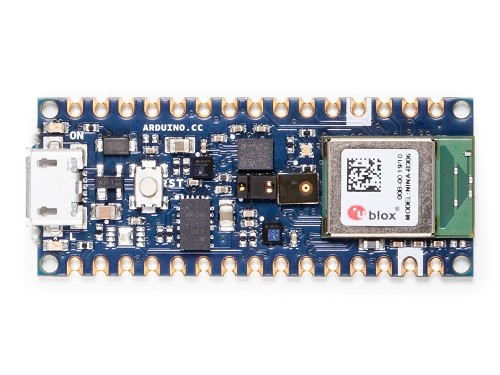
\includegraphics[width=\linewidth]{Images/HardwareDescription/ArduinoTop}
	\caption{\textbf{Top View of Board Arduino Nano 33 BLE Sense}}
	\label{fig:Top View of Board Arduino Nano 33 BLE Sense}
	\cite{Arduino:2023}
\end{figure}

\begin{figure}[h!]
	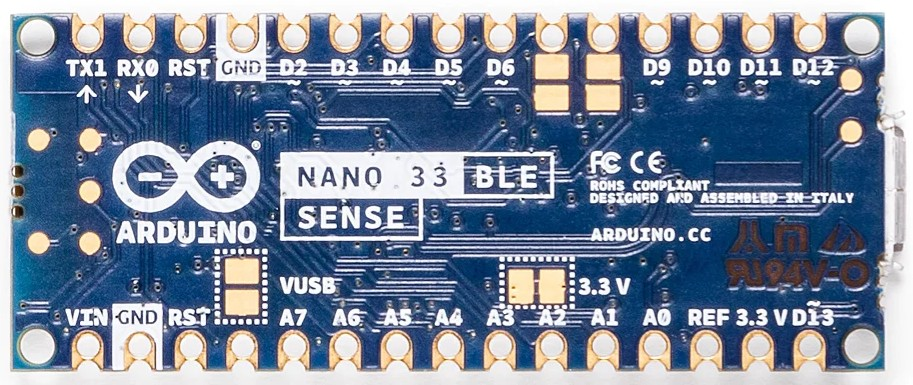
\includegraphics[width=\linewidth]{Images/HardwareDescription/ArduinoBottom}
	\caption{\textbf{Bottom View of Board Arduino Nano 33 BLE Sense}}
	\label{fig:Bottom View of Board Arduino Nano 33 BLE Sense} \cite{Arduino:2023}
\end{figure}


\section{Interfaces}

\subsection{Board Arduino Nano 33 BLE Sense: Components Overview}\label{BoardDescription}



The Arduino Nano 33 BLE Sense is equipped with several embedded sensors, including humidity, temperature, barometric pressure, proximity, and a microphone. These built-in components allow the board to be utilized for various practical applications without the need for additional circuitry \cite{Arduino:2021}. It supports standard communication protocols such as UART, I2C, and SPI, enabling seamless interaction with external circuits and sensors for data exchange. The board includes a micro-USB port for connecting to a laptop or desktop, which serves as both a power supply and a medium for file or data transfer via serial communication. While operating the board, it is crucial to ensure that no more than 3.3V is applied to its pins, as exceeding this voltage can result in permanent damage \cite{Arduino:2021}.

Below is a detailed description of each sensor embedded on the board:

\begin{center}
	\begin{tikzpicture}
		\ArduinoNanoTikz
		
		\node(HTS) at (-10,5){\textcolor{red}{\tiny HTS221}};
		\draw[line width=1pt,red]  (-6.3,2.8) -- (-10,4.9);
		\node(APD) at (-6,5){\textcolor{red}{\tiny APDS9960}};
		\draw[line width=1pt,red]  (-5,2.25) -- (-6,4.9);
		\node(LSM9DS1) at (-2,5){\textcolor{red}{\tiny LSM9DS1}};
		\draw[line width=1pt,red]  (-5,3.15) -- (-2,4.9);
		
		\node(LSM9DS1) at (1,5){\textcolor{red}{\tiny RGB Programmable LED}};
		\draw[line width=1pt,red]  (-3.6,2.95) -- (1,4.9);
		
		\node(HTS) at (1.5,2.25){\textcolor{red}{\tiny Nordic nRF 52840}};
		\draw[line width=1pt,red]  (-2,2.25) -- (0.5,2.25);
		
		\node(MP) at (-2,-0.75){\textcolor{red}{\tiny MP34DT05-A}};
		\draw[line width=1pt,red]  (-3.9,2.25) -- (-1.75,-0.6);
		
		\node(MP) at (-6,-0.75){\textcolor{red}{\tiny LPS22HB}};
		\draw[line width=1pt,red]  (-4.5,1.0) -- (-6,-0.6);
		
		\node(LEDPower) at (-11.5,3.55){\textcolor{red}{\tiny Power LED}};
		\draw[line width=1pt,red]  (-10.8,3.55) -- (-10,3.55);
		
		\node(USB) at (-12,2.25){\textcolor{red}{\tiny Micro-USB Port}};
		\draw[line width=1pt,red]  (-11.1,2.25) -- (-10.2,2.25);
		
		\node(LEDOrange) at (-11.8,0.8){\textcolor{red}{\tiny Progammable LED}};
		\draw[line width=1pt,red]  (-10.8,0.8) -- (-10,0.8);
		
	\end{tikzpicture}
	\captionof{figure}{}\label{ArduinoNano33BLESenseArchitecture}
\end{center}

\begin{itemize}
	\item LSM9DS1 - \ac{imu} features a 3D accelerometer, gyroscope and magnetometer and allows you to detect orientation, motion or vibrations in your project \cite{Alushi:2023}.
	\item  APDS-9960 - The APDS-9960 chip allows for measuring digital proximity and ambient light as well as for detecting RGB colors and gestures \cite{Avago:2015}.
	\item  LPS22HB - The LPS22HB picks up on barometric pressure and allows for a 24-bit pressure data output between 260 and 1260 hPa. This data can also be processed to calculate the height above sea level of the current location \cite{Stm:2017}.
	\item HTS221 - The HTS221 capacitive digital sensor measures relative humidity and temperature. It has a temperature accuracy of ± 0.5 °C (between 15-40 °C) and is perfectly suited to detect ambient temperature \cite{Stm:2023}.
	\item MP34DT05 - The MP34DT05 microphone allows you to capture and analyze sound in real-time and can be used to create a voice interface for your project\cite{Stm:2021}.
	\item USB port - USB port allows you to connect Arduino Nano 33 BLE sense to your machine.
	\item LEDs - There are 3 different LEDs that can be accessed on the Nano BLE Sense: \ac{rgb}(Programmable LED), the built-in LED(Programmable LED) and the power LED
\end{itemize}

\subsubsection{LEDs function in Board Arduino Nano 33 BLE Sense}
Apart from the Power LED indicate the board is powered, there are two LEDs in the board: Programmable LED(orange) and the RGB Programmable LED. The orange LED sparkles when it is connected to the computer. The RGB LED can be used during the creation of the actions that we perform. For example, in our project, each gesture can use one color to represent a specific gesture, indicating as the recognizing function. 

\section{Arduino Nano 33 BLE Pin Configuration}

The \textbf{Arduino Nano 33 BLE} is an advanced version of the Arduino Nano board that is based on a powerful processor, the nRF52840. The following is the pin configuration of the board:

\subsection{Pin Configuration}
\textbf{Digital Pins:}
\begin{itemize}[noitemsep]
	\item The board has \textbf{14 digital I/O pins} that receive only two values: HIGH or LOW.
	\item These pins can function as input or output based on the requirement.
	\item When the pins receive 5V, they are in a HIGH state; when they receive 0V, they are in a LOW state.
\end{itemize}

\textbf{Analog Pins:}
\begin{itemize}[noitemsep]
	\item The board has a total of \textbf{8 analog pins} (A0–A7).
	\item These pins measure analog voltage ranging between 0 to 5V and can get any value as opposed to digital pins, which only receive HIGH or LOW values.
\end{itemize}

\textbf{PWM Pins:}
\begin{itemize}[noitemsep]
	\item All digital pins can be used as PWM pins.
	\item These pins generate analog results using digital means.
\end{itemize}

\textbf{SPI Pins:}
\begin{itemize}[noitemsep]
	\item The board supports the \textbf{Serial Peripheral Interface (SPI)} communication protocol.
	\item SPI is used to communicate between the controller and peripheral devices such as shift registers and sensors.
	\item Two pins, \textbf{MISO} (Master Input Slave Output) and \textbf{MOSI} (Master Output Slave Input), are used for SPI communication.
\end{itemize}

\textbf{I2C Pins:}
\begin{itemize}[noitemsep]
	\item The board supports the \textbf{I2C communication protocol}, a two-wire protocol.
	\item It includes two pins: \textbf{SDL} and \textbf{SCL}.
\end{itemize}

\textbf{UART Pins:}
\begin{itemize}[noitemsep]
	\item The board features the \textbf{UART communication protocol} for serial communication.
	\item It includes two pins: \textbf{Rx} (receiving pin) and \textbf{Tx} (transmitting pin).
\end{itemize}

\textbf{External Interrupts Pins:}
\begin{itemize}[noitemsep]
	\item All digital pins can be used as external interrupt pins.
	\item This feature allows the main running program to be interrupted and handle emergency instructions.
\end{itemize}

\textbf{LED at Pin 13 and AREF Pin:}
\begin{itemize}[noitemsep]
	\item There is an \textbf{LED connected to pin 13} of the board.
	\item The \textbf{AREF pin} is used as a reference voltage for input voltage.
\end{itemize}

\begin{figure}[h!]
	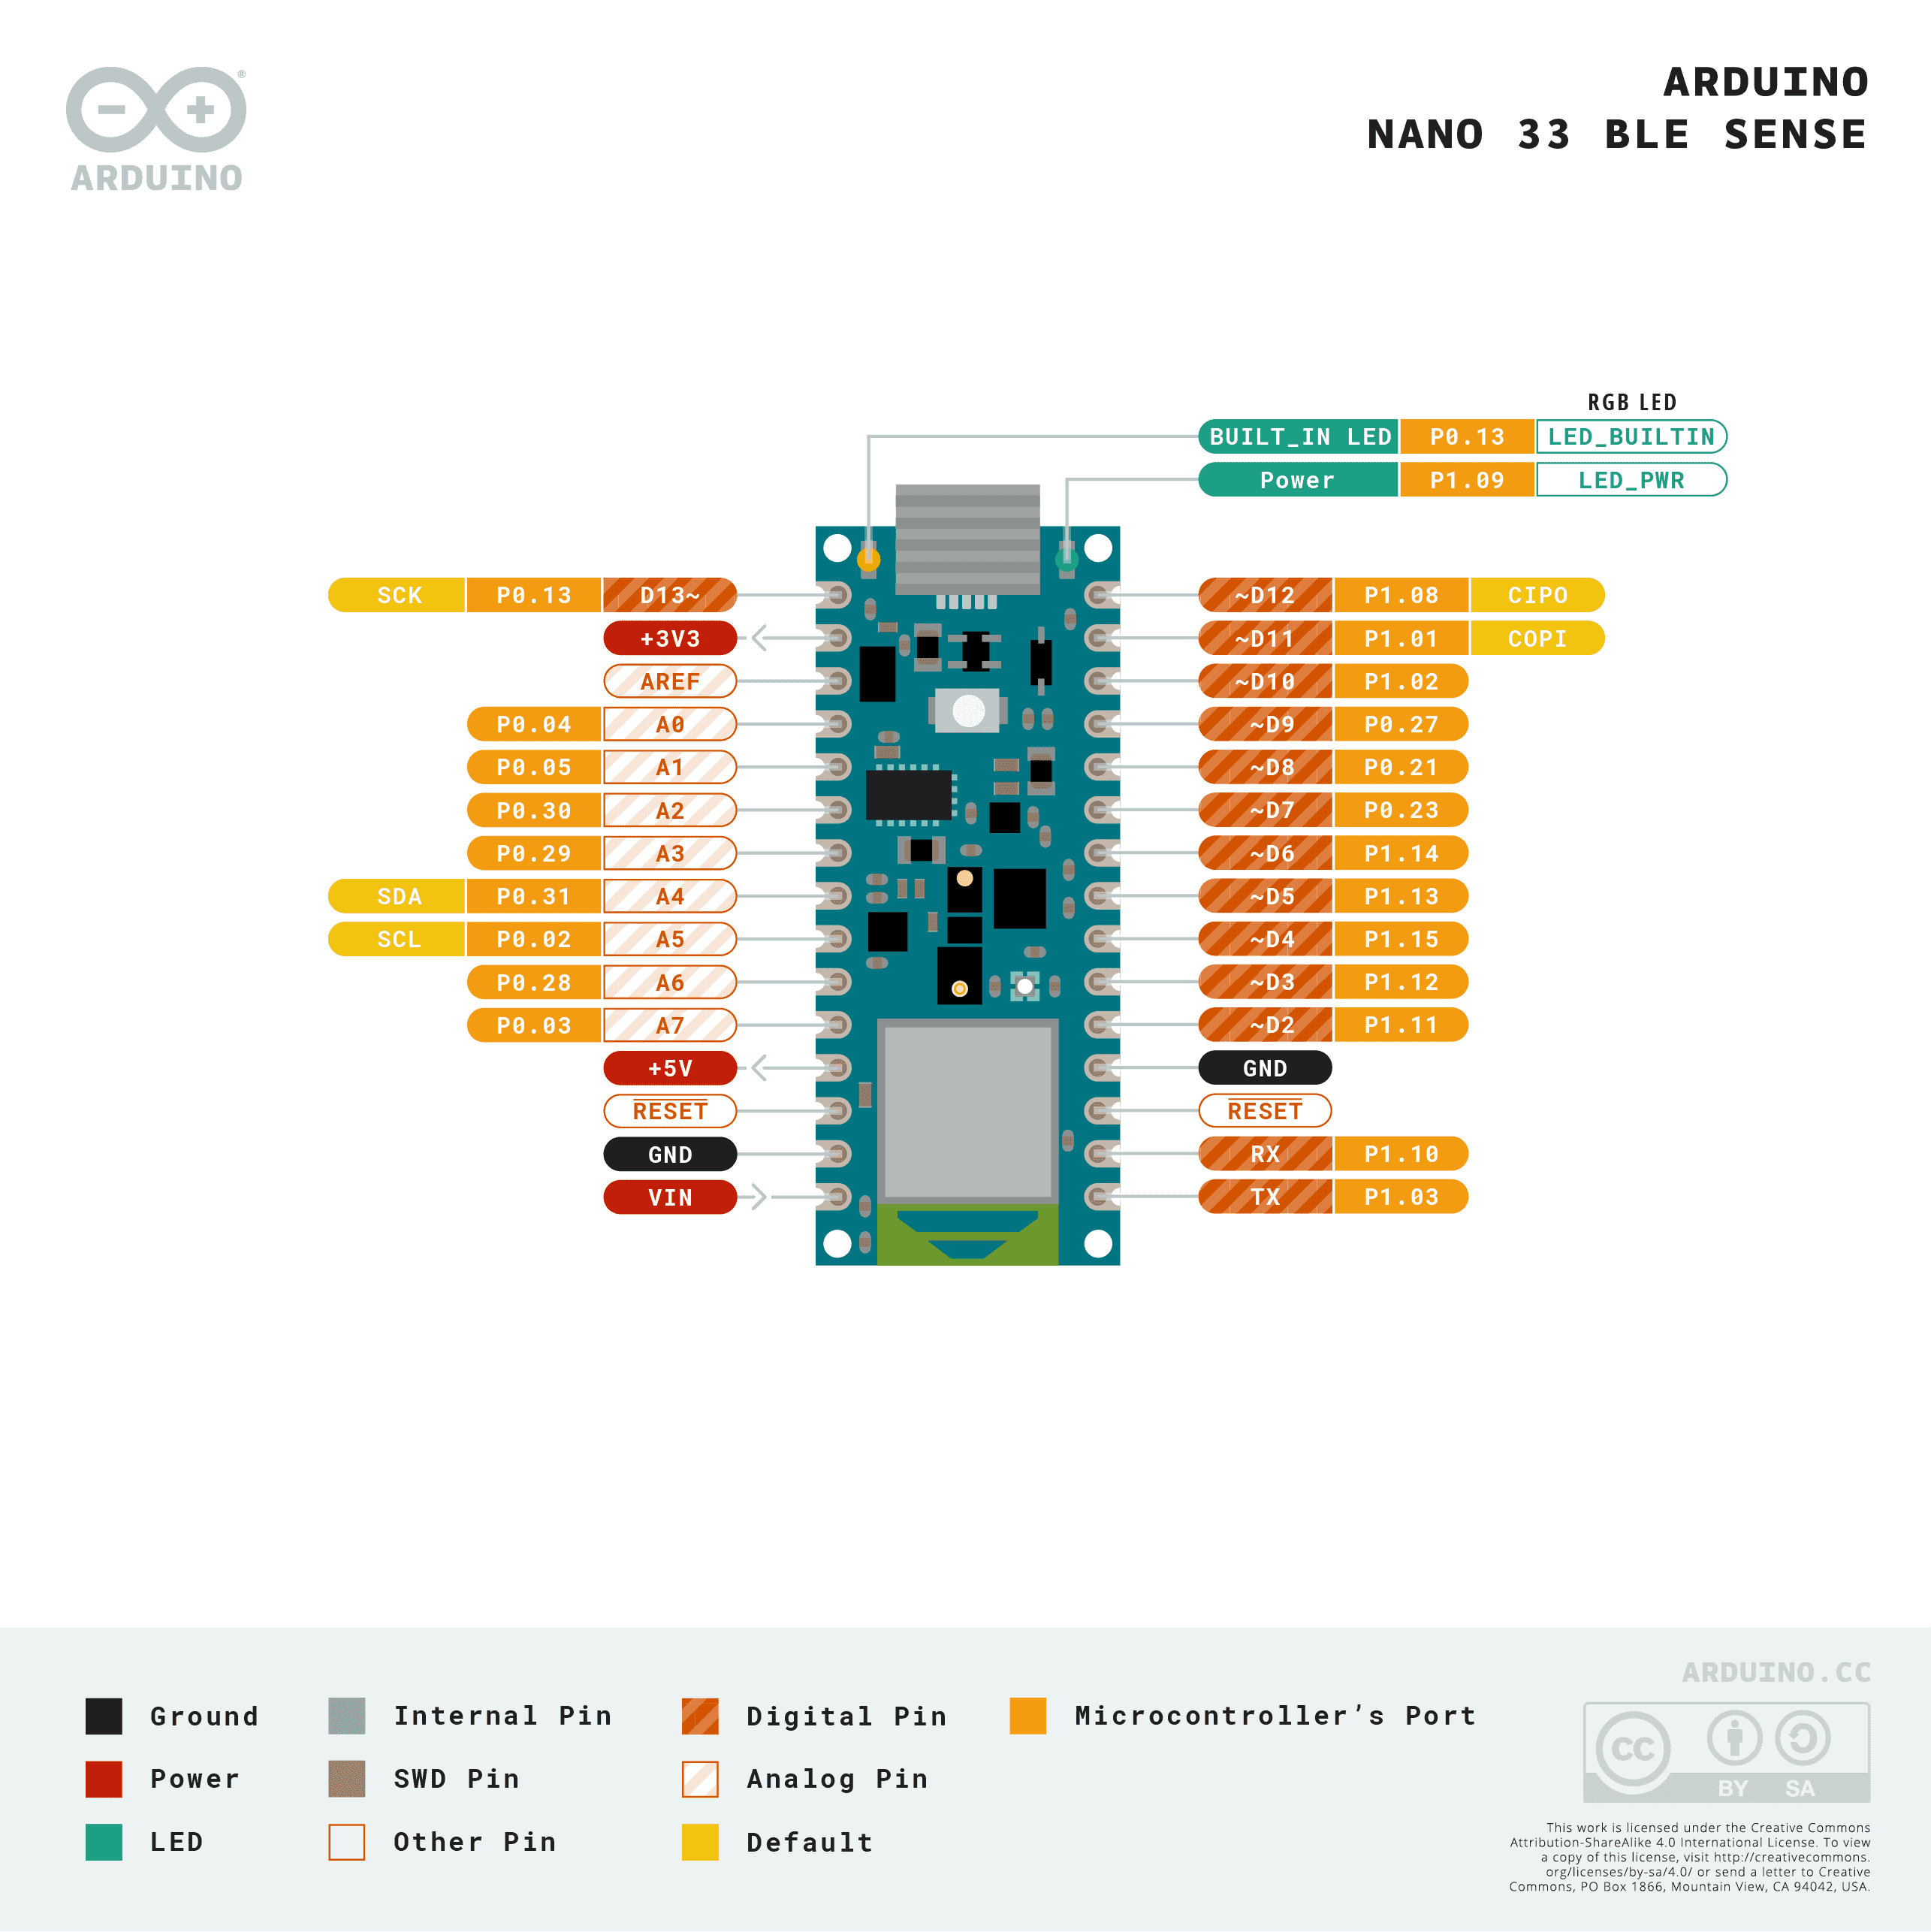
\includegraphics[width=\linewidth]{Images/HardwareDescription/Pin_Configuration}
	\caption{\textbf{Arduino Nano 33 BLE Pin Configuration}}
	\label{Arduino Nano 33 BLE Pin Configuration} \cite{Arduino:2023}
\end{figure}

\section{Data Quality in Hardware Description}

In the hardware description of our Magic Wand project with Arduino Nano 33 BLE Sense, we consider the following aspects related to data quality:

\begin{enumerate}
	\item \textbf{Sensor Accuracy:} The sensors embedded in the Arduino Nano 33 BLE Sense board deliver precise measurements of environmental parameters such as motion, orientation, temperature, humidity, and pressure \cite{Dhow:2024}.
	
	\item \textbf{Resolution:} Each sensor has a defined resolution, representing the smallest detectable input change. For instance, the accelerometer’s resolution is \textless{}insert value\textgreater{}, allowing detection of subtle motion variations.
	
	\item \textbf{Sampling Rate:}The board supports high sampling rates, enabling real-time data acquisition at \textless{}insert frequency\textgreater{} Hz. This is essential for applications requiring continuous and responsive data collection.
	
	\item \textbf{Noise Level:} Sensor data may exhibit noise due to factors such as environmental conditions, sensor imperfections, or electromagnetic interference. The board minimizes noise using calibration and filtering techniques, ensuring high data fidelity.
	
	\item \textbf{Calibration:} Calibration processes are applied to enhance the accuracy and reliability of sensor readings. These procedures involve fine-tuning sensor settings and using correction factors to address systematic errors \cite{Edm:2015}.
	
	\item \textbf{Data Transmission:} Sensor data is transmitted from the Arduino Nano 33 BLE Sense board to other devices using wireless communication protocols such as Bluetooth Low Energy (BLE). Data transmission is efficient, ensuring minimal latency and reliable delivery.
	
	\item \textbf{Data Integrity:} To maintain data integrity during transmission and processing, error detection and correction mechanisms are implemented. These measures help identify and resolve issues like data loss or corruption \cite{TensorFlow:2023}.
	
	\item \textbf{Power Consumption:} The Arduino Nano 33 BLE Sense is designed for low power consumption, making it ideal for battery-powered applications. Its optimized power management extends battery life without compromising continuous data collection.
\end{enumerate}

By addressing these aspects of data quality in the hardware description, we ensure the reliability and accuracy of sensor data used in our Magic Wand project.
\begin{center}
	\begin{tikzpicture}
		
		\ArduinoNanoTikz
		
		\node[rotate=90,right] (Pin1) at (-0.91,4.6) {(1) \; D1/TX};
		\node[rotate=90,right] (Pin2) at (-1.56,4.6) {(2) \; D0/RX};
		\node[rotate=90,right] (Pin3) at (-2.11,4.6) {(3) \; Reset};
		\node[rotate=90,right] (Pin4) at (-2.76,4.6) {(4) \; GND};
		\node[rotate=90,right] (Pin5) at (-3.36,4.6) {(5) \; $\sim$D2};
		\node[rotate=90,right] (Pin6) at (-3.96,4.6) {(6) \; $\sim$D3};
		\node[rotate=90,right] (Pin7) at (-4.56,4.6) {(7) \; $\sim$D4};
		\node[rotate=90,right] (Pin8) at (-5.16,4.6) {(8) \; $\sim$D5};
		\node[rotate=90,right] (Pin9) at (-5.76,4.6) {(9) \; $\sim$D6};
		\node[rotate=90,right] (Pin10) at (-6.36,4.6) {(10) \; $\sim$D7};
		\node[rotate=90,right] (Pin11) at (-6.96,4.6) {(11) \; $\sim$D8};
		\node[rotate=90,right] (Pin12) at (-7.56,4.6) {(12) \; $\sim$D9};
		\node[rotate=90,right] (Pin13) at (-8.16,4.6) {(13) \; $\sim$D10};
		\node[rotate=90,right] (Pin14) at (-8.76,4.6) {(14) \; $\sim$D2/MOSI};
		\node[rotate=90,right] (Pin15) at (-9.36,4.6) {(15) \; $\sim$D2/MISO};
		
		
		\node[rotate=90,left] (Pin30) at (-0.91,-0.4) { $V_{in}$ \; (30)};
		\node[rotate=90,left] (Pin1) at (-1.56,-0.4) {GND \; (29)};
		\node[rotate=90,left] (Pin2) at (-2.11,-0.4) {Reset \; (28)};
		\node[rotate=90,left] (Pin3) at (-2.76,-0.4) {+5V \; (27)};
		\node[rotate=90,left] (Pin4) at (-3.36,-0.4) {A7 \; (26)};
		\node[rotate=90,left] (Pin5) at (-3.96,-0.4) {A6 \; (25)};
		\node[rotate=90,left] (Pin6) at (-4.56,-0.4) {SCL/A5 \; (24)};
		\node[rotate=90,left] (Pin7) at (-5.16,-0.4) {SDA/A4 \; (23)};
		\node[rotate=90,left] (Pin8) at (-5.76,-0.4) {A3 \; (22)};
		\node[rotate=90,left] (Pin9) at (-6.36,-0.4) {A2 \; (21)};
		\node[rotate=90,left] (Pin10) at (-6.96,-0.4) {A1 \; (20)};
		\node[rotate=90,left] (Pin11) at (-7.56,-0.4) {A0 \; (19)};
		\node[rotate=90,left] (Pin12) at (-8.16,-0.4) {AREF \; (18)};
		\node[rotate=90,left] (Pin13) at (-8.76,-0.4) {+3V3 \; (17)};
		\node[rotate=90,left] (Pin14) at (-9.36,-0.4) {SCK/$\sim$D13 \; (16)};
		
	\end{tikzpicture}
	\captionof{figure}[Pin assignment of the Arduino Nano 33 BLE Sense]{Pin assignment of the Arduino Nano 33 BLE Sense; note that the orange built-in LED is connected to pin D13 and the power LED to pin D1. The built-in RGB LED occupies pins D18, D19 and D20.}
\end{center}

\subsection{Specifications of Arduino Nano 33 BLE Sense}


\subsubsection*{NINA B306 Module}
\begin{enumerate}[label=\arabic*.]
	\item Processor:
	\begin{itemize}[label=-]
		\item 64 MHz Arm® Cortex-M4F (with FPU)
		\item 1 MB Flash + 256 KB RAM
	\end{itemize}
	\item Bluetooth® 5 multiprotocol radio:
	\begin{itemize}[label=-]
		\item 2 Mbps
		\item +8 dBm TX power
		\item -95 dBm sensitivity
		\item 4.8 mA in TX (0 dBm)
		\item 4.6 mA in RX (1 Mbps)
		\item Integrated balun with 50 Ohm single-ended output
		\item IEEE 802.15.4 radio support
	\end{itemize}
	\item Peripherals:
	\begin{itemize}[label=-]
		\item 12 Mbps USB
		\item NFC-A tag
		\item Arm CryptoCell CC310 security subsystem
		\item QSPI/SPI/TWI/I2S/PDM/QDEC
		\item 32 MHz SPI
		\item Quad SPI interface 32 MHz
		\item 12-bit 200 ksps ADC
		\item 128 bit AES/ECB/CCM/AAR co-processor
	\end{itemize}
\end{enumerate}

\subsubsection*{LSM9DS1 (9 axis IMU)}\cite{Warden:2020}
\begin{enumerate}[label=\arabic*.]
	\item 3 acceleration channels, 3 angular rate channels, 3 magnetic field channels
	\item $\pm$2/$\pm$4/$\pm$8/$\pm$16 g linear acceleration full scale
	\item $\pm$4/$\pm$8/$\pm$12/$\pm$16 gauss magnetic full scale
	\item $\pm$245/$\pm$500/$\pm$2000 dps angular rate full scale
	\item 16-bit data output
\end{enumerate}




\section{Data quantity in Hardware Description}

\begin{enumerate}
	\item \textbf{Sensor Data}: The Arduino Nano 33 BLE Sense board is equipped with a variety of sensors, including an accelerometer, a gyroscope, and a magnetometer. These sensors generate a large amount of data as you wave the magic wand. For instance, in one experiment, a window size of 2 seconds was used, which means 200 rows of accelerometer data or 600 values of x, y, and z acceleration axis were fed into the model. \cite{Miller:2022}
	
	\item \textbf{Data Processing Capacity}: The Arduino Nano 33 BLE Sense board has a 32-bit ARM Cortex-M4 CPU running at 64 MHz, which allows it to process a significant amount of sensor data in real-time.
	
	\item \textbf{Memory}: The board has 1MB of flash memory and 256KB of SRAM. This memory is used to store the program code and handle runtime operations, including storing sensor data and machine learning model parameters.
	
	\item \textbf{Machine Learning Model}: The size of the machine learning model used in the project also affects the quantity of data. The model needs to be small enough to fit into the board's memory along with the program code.
	
	\item \textbf{Data Transmission}: The board also has a built-in Bluetooth Low Energy module, which can be used to transmit sensor data to another device for further processing. \cite{TensorFlow:2023}
	
\end{enumerate}


\section{Constraints}
\subsubsection{Arduino Nano 33 BLE Sense}
\begin{itemize}[label=--]
	\item Operating Voltage: 3.3V
	\item Power Consumption:
	\begin{itemize}[label=--,leftmargin=*]
		\item Maximum 15mA in low power mode
		\item Maximum 60mA in active mode
	\end{itemize}
	\item Operating Temperature Range: -40°C to 85°C
	\item Memory Constraints: 1 MB Flash + 256 KB RAM
	\item Communication Interfaces: USB, Bluetooth 5, NFC-A, SPI, I2C, QSPI, etc.\cite{Arduino:2015}
\end{itemize}

\subsubsection*{Sensors}
\begin{itemize}[label=--]
	\item Accelerometer:
	\begin{itemize}[label=--,leftmargin=*]
		\item Measurement Range: ±8g
		\item Operating Temperature Range: -40°C to 85°C
	\end{itemize}
	\item Gyroscope:
	\begin{itemize}[label=--,leftmargin=*]
		\item Measurement Range: ±2000 dps
		\item Operating Temperature Range: -40°C to 85°C \cite{Arduino:2021}
	\end{itemize}
	
\end{itemize}


\subsubsection*{Actuators}
\begin{itemize}[label=--]
	\item RGB LEDs:
	\begin{itemize}[label=--,leftmargin=*]
		\item Power Requirements: Voltage, Current
		\item Operating Temperature Range
	\end{itemize}
	\item Buzzer/Speaker:
	\begin{itemize}[label=--,leftmargin=*]
		\item  Voltage, Current, Sound Output Levels
	\end{itemize}
	
\end{itemize}

\subsubsection*{Power Supply}
\begin{itemize}[label=--]
	\item Input Voltage Range: Specify the acceptable input voltage range.
	\item Power Consumption: Estimate the overall power consumption of the system.
\end{itemize}

\subsubsection*{Physical Constraints}
\begin{itemize}[label=--]
	\item Size and Dimensions: Ensure compatibility with the project enclosure or housing.
	\item Mounting Requirements: Specify any specific mounting requirements for the components.
\end{itemize}

\subsubsection*{Environmental Constraints}
\begin{itemize}[label=--]
	\item Environmental Protection: Ensure components are suitable for the intended environmental conditions (e.g., moisture resistance, dust resistance).
	\item Operating Conditions: Specify any limitations or special considerations for operating in certain environments.\cite{Arduino:2021}
\end{itemize}



\section{Dimensions of the Arduino Nano 33 BLE Sense}



The Arduino Nano 33 BLE Sense is a highly compact development board, measuring just 45mm x 18mm. Its small form factor makes it particularly well-suited for wearable devices and other space-constrained applications. Despite its size, the board is equipped with a wide range of sensors and features, offering versatility for various projects.

It is important to note that these dimensions apply to the board without headers. If you are using a version with pre-soldered headers or attaching additional components, the overall dimensions of your hardware setup may change. For precise measurements, always consult the specifications of your specific board and components \cite{Arduino:2023}.


\section{Sensor Accelerometer, Gyroscope, and Magnetometer LSM9DS1}\label{boardsensor}

Magic Wand gesture detection is mainly based on the sensor LSM9DS1 at the board. It is a system-in-package featuring a 3D digital linear acceleration sensor, a 3D digital angular rate sensor, and a 3D digital magnetic sensor. A tiny device called an Inertial Measurement Unit (IMU) in the sensor is used to detect the motions physically \cite{Alushi:2023}. It has several components, including magnetometer, gyroscope, and accelerometer. By monitoring  acceleration and angular velocity changes, the IMU sensor is critical for identifying an object's orientation and movement in real-time \cite{Alushi:2023}.





\subsection*{Example Code for Arduino Nano 33 BLE Sense}
Below is a simple example demonstrating how to use the built-in microphone on the Arduino Nano 33 BLE Sense:

\begin{code}
	\begin{Arduino}
		// Include the PDM library
		#include <PDM.h>
		
		// Buffer to store the microphone data
		short sampleBuffer[256];
		
		// Variable to store the sound level
		int soundLevel = 0;
		
		// Callback function for PDM data
		void onPDMdata() {
			// Read the PDM data
			int bytesAvailable = PDM.available();
			PDM.read(sampleBuffer, bytesAvailable);
			
			// Calculate the sound level
			soundLevel = 0;
			for (int i = 0; i < bytesAvailable / 2; i++) {
				soundLevel += abs(sampleBuffer[i]);
			}
			soundLevel /= bytesAvailable / 2;
		}
		
		void setup() {
			// Initialize serial communication
			Serial.begin(9600);
			while (!Serial);
			
			// Initialize PDM with a sample rate of 16 kHz and 16-bit resolution
			PDM.begin(1, 16000);
			PDM.onReceive(onPDMdata);
		}
		
		void loop() {
			// Print the sound level to the serial monitor
			Serial.println(soundLevel);
			delay(100);
		}
	\end{Arduino}
	\caption{Simple example using of the builtin microphone of the Arduino Nano 33 BLE Sense}\label{code:microphone}
\end{code}

\begin{code}
	\begin{Arduino}
		// Include the ArduinoBLE library
		#include <ArduinoBLE.h>
		
		// Create a BLE service
		BLEService batteryService("1101");
		
		// Create a BLE characteristic
		BLEUnsignedCharCharacteristic batteryLevelChar("2101", BLERead | BLENotify);
		
		void setup() {
			// Initialize serial communication
			Serial.begin(9600);
			while (!Serial);
			
			// Set up the built-in LED pin
			pinMode(LED_BUILTIN, OUTPUT);
			
			// Initialize BLE
			if (!BLE.begin()) {
				Serial.println("Starting BLE failed!");
				while (1);
			}
			
			// Set the BLE local name and advertised service
			BLE.setLocalName("BatteryMonitor");
			BLE.setAdvertisedService(batteryService);
			
			// Add characteristic to the service
			batteryService.addCharacteristic(batteryLevelChar);
			
			// Add the service and start advertising
			BLE.addService(batteryService);
			BLE.advertise();
			
			Serial.println("Bluetooth device active, waiting for connections...");
		}
		
		void loop() {
			// Wait for a BLE central to connect
			BLEDevice central = BLE.central();
			
			if (central) {
				Serial.print("Connected to central: ");
				Serial.println(central.address());
				
				// Turn on the built-in LED
				digitalWrite(LED_BUILTIN, HIGH);
				
				// Loop while the central device is connected
				while (central.connected()) {
					int battery = analogRead(A0);
					int batteryLevel = map(battery, 0, 1023, 0, 100);
					
					Serial.print("Battery Level is now: ");
					Serial.println(batteryLevel);
					
					// Update the characteristic value
					batteryLevelChar.writeValue(batteryLevel);
					
					delay(200);
				}
				
				// Turn off the built-in LED
				digitalWrite(LED_BUILTIN, LOW);
				Serial.print("Disconnected from central: ");
				Serial.println(central.address());
			}
		}
	\end{Arduino}
	\caption{Example of a BLE Battery Monitor using Arduino Nano 33 BLE Sense}\label{code:battery-monitor}
\end{code}

\pagebreak
\section{Inertial Measurement Unit (IMU)}\label{IMU}

\subsection{Description}
An Inertial Measurement Unit (IMU) is an electronic system that measures movement across multiple axes using three primary sensors: an accelerometer, a gyroscope, and a magnetometer.\cite{Qureshi:2017} These sensors work together to provide data on acceleration, rotational motion, and magnetic fields, making IMUs essential for a wide range of applications such as navigation, fitness tracking, and robotics.\cite{Qureshi:2017}

{General}
IMUs have become increasingly common in microcontroller projects, with some boards, such as the Arduino Nano 33 BLE Sense, featuring integrated IMUs for seamless development of motion-sensitive applications.\cite{Zhou:2020}

\subsection{Specific Sensors}
\textbf{Continuous Operation ("Always-On" Mode)}
The LSM9DS1 supports an "Always-On" mode, ensuring continuous operation even when the main system is in a low-power state.\cite{Zhou:2020} This is critical for uninterrupted motion monitoring in devices like the Magic Wand, where gestures must be tracked instantly. With a power consumption of just 0.55 mA in high-performance mode, it provides precise and reliable motion data while preserving battery life.\cite{Zhou:2020}

\textbf{Tilt Detection}
Using the accelerometer, the IMU can detect orientation changes with minimal power usage. Tilt detection is particularly useful for identifying subtle shifts in position, enhancing the responsiveness of gesture-based controls.\cite{Zhou:2020}

\textbf{Significant Motion Detection}
The accelerometer enables significant motion detection (SMD), which recognizes large-scale movements. SMD can be used to activate specific device functions, such as waking the system from sleep mode or triggering predefined actions based on significant gestures.\cite{Zhou:2020}

The LSM9DS1 is a versatile and energy-efficient IMU with advanced sensing capabilities, supporting a range of applications where motion detection, orientation tracking, and gesture recognition are essential. Its compact design, low power consumption, and robust environmental tolerance make it a reliable choice for portable, battery-powered devices like the Magic Wand.\cite{Zhou:2020}

An \ac{imu} consists of three sensors that measure an object's orientation, position, vibration and movement in 3D space in real-time. These sensors are typically arranged in a pattern, including a tri-axial accelerometer, gyroscope, and magnetometer\cite{Ahmad:2013}. An accelerometer is used to measure the change in velocity of a moving or vibrating object\cite{Ahmad:2013}. Gyroscope measures the angular rotation\cite{Ahmad:2013}. A Magnetometer is used to measure yaw angle rotation, calibrating to the gyroscope data to improve the big drift issue\cite{Ahmad:2013}. 

The accelerometer functions by gauging the acceleration (Ax, Ay, Az), which denotes the rate of acceleration change over time. The acceleration values along each axis are conventionally expressed in units of meters per second squared $(m/s^2)$ \cite{Vernier:2023}. To illustrate, if the LSM9DS1 records an acceleration of 15 $m/s^2$ along the x-axis, this signifies that the object under observation is experiencing a velocity increment of 15 meters per second every second in the x-direction.

A gyroscope, designed to quantify angular speed ($\omega$x, $\omega$y, $\omega$z), serves as an indicator of the object's orientation change rate along each axis. Angular velocity along each axis is commonly expressed in degrees per second ($\circ$/s) \cite{Zhuang:2020}. For instance, when the LSM9DS1 records an angular velocity of 100$\circ$/s along the z-axis, it signifies that the measured object is undergoing rotation at a rate of 100 degrees per second around the z-axis. Refer to the accompanying figure for visualization.

In the context of a magnetometer, the x, y, and z axes (Mx, My, Mz) typically delineate the three-dimensional space in which the magnetic field is being assessed. The x-axis typically corresponds to the horizontal component of the magnetic field, the y-axis signifies the vertical component, and the z-axis reflects the magnetic field strength \cite{Kostiainen:2023}. This three-dimensional measurement provides a comprehensive understanding of the magnetic field in the surrounding space.

\begin{figure}[h!]\centering
	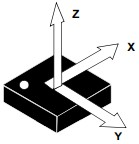
\includegraphics[width=6cm]{Images/HardwareDescription/AccelerometerForce}
	\caption{\textbf{Accelerometer Accerlerations Directions}}
	\label{fig:Acceleromter}
	\cite{Stm:2015}
\end{figure}

\begin{figure}[h!]\centering
	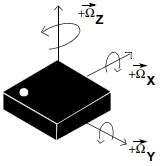
\includegraphics[width=6cm]{Images/HardwareDescription/AngularRotation}
	\caption{\textbf{Gyroscope Angular Directions}}
	\label{fig:Gyroscope}
	\cite{Stm:2015}
\end{figure}

\begin{figure}[h!]\centering
	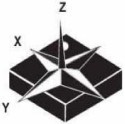
\includegraphics[width=6cm]{Images/HardwareDescription/MagnetometerDirection}
	\caption{\textbf{Magnetometer Directions}}
	\label{fig:Magnetometer}
	\cite{Stm:2015}
\end{figure}

IMUs can be classified into two main categories based on the type of sensors used: \ac{mems} IMUs and \ac{FOG} IMUs. MEMS IMUs use small mechanical sensors that are etched onto a silicon chip, while FOG IMUs use optical fibers to measure angular velocity. MEMS IMUs are typically smaller and less expensive but are also less accurate and have a shorter lifespan compared to FOG IMUs\cite{Deppe:2017}.

IMU is sent to a microcontroller or computer, and software is written to read the data from the sensors and perform the necessary calculations. There are also many libraries and software packages available that can simplify the process of working with IMUs.

IMUs are commonly used in a variety of applications, Industry Quality Control, Medical Rehabilitation, Robotics, Navigation Systems, Sports Learning and Augmented Reality Systems since they are essential to accurately measure the movement and orientation of the device for further function development \cite{Ahmad:2013}. In general, they are used for: 

\textbf{Orientation tracking:} IMUs can follow the orientation of an object in space by using a combination of acceleration and angular velocity sensors. The data from these sensors can be used to calculate the object's orientation. Robotics technology is one of the regions that require linear and angular data for the movements so robots can perform daily routines and advanced tasks similar to humans \cite{Ahmad:2013}.  

\textbf{Motion sensing:}  Detecting motion and acceleration changes is also one function that IMUs can achieve. Ryan et al. suggested integrating a miniaturized IMU sensor into the ball, comprising a tri-axial gyroscope and tri-axial accelerometer. Their initial experiment employed ball kinematics knowledge to estimate the drift error arising from measurements \cite{McGinnis:2011}. Subsequent research efforts enhanced data accuracy by cross-referencing the measurements with a high-speed motion analysis system consisting of 10 cameras (VICON) \cite{McGinnis:2012}.

\textbf{Navigation System:} IMUs are marked as an upgrade in the Global Positioning System (GPS) to navigate by combining data from the acceleration and angular velocity sensors with information for better data accuracy. Also, IMU can provide locations where no GPS signals are detected as an alternative option in the car and aircraft in case of emergency \cite{Ahmad:2013}. 

However, IMUs face a significant challenge due to the susceptibility of the underlying gyroscopes and accelerometers to measurement errors. This poses a fundamental issue for all IMUs as gyroscopes inherently exhibit drift, and accelerometers may introduce inaccuracies, resulting in misestimations of orientation concerning gravity. Despite incorporating minor measurement errors, the guidance system continually integrates the calculated position results with the original position information (refer to trajectory calculation). Although individual errors may be minor, their persistence across positions leads to cumulative effects known as "drift." Over time, this accumulation causes a widening disparity between the system's perceived and actual locations, and it becomes impossible to eliminate these errors \cite{Harris:2023}. Therefore, drift remains a fundamental challenge for any IMUs.
\subsection{Specifications}
\begin{itemize}
	\item 3 acceleration channels, 3 angular rate channels, 3 magnetic field channels.
	\item $\pm2/\pm4/\pm8/\pm16$ g linear acceleration full scale.
	\item $\pm4/\pm8/\pm12/\pm16$ gauss magnetic full scale.
	\item $\pm245/\pm500/\pm2000$ dps angular rate full scale.
	\item 16-bit data output.
\end{itemize}

3D digital linear acceleration sensor: Measures linear motion with a full scale of ±2g/±4g/±8g/±16g.\newline
3D digital angular rate sensor: Tracks rotational motion with an angular rate range of ±245/±500/±2000 degrees per second (dps).\newline
3D digital magnetic sensor: Detects magnetic fields with a full scale of ±4/±8/±12/±16 gauss.\newline
This compact and versatile IMU includes both I²C and SPI serial interfaces and supports a power-down mode for smart power management. It is available in a plastic land grid array (LGA) package and operates reliably across a wide temperature range from -40 °C to +85 °C.

\subsection{Libraries}

A library refers to a collection of pre-written code that can be used by developers to perform specific tasks or functions without having to write the code from scratch. Libraries are designed to make the development process easier and more efficient by providing pre-built solutions to common programming challenges.

\subsubsection{Wire.h}
\texttt{Wire.h} is a library in Arduino that allows for communication between I2C devices. I2C stands for Inter-Integrated Circuit, which is a synchronous serial communication protocol used for connecting microcontrollers to peripheral devices. \texttt{Wire.h} provides functions for initializing the I2C bus, sending and receiving data over the bus, and managing multiple devices on the same bus. With this library, developers can easily connect multiple I2C devices, such as sensors or displays, to an Arduino board \cite{Ardc; Ari21}.

\subsubsection{Kalman.h}
\texttt{Kalman.h} is a library that implements the Kalman filter algorithm. The Kalman filter is a mathematical technique used to estimate the state of a system based on incomplete measurements. It is commonly used in control systems, robotics, and navigation applications to improve the accuracy of sensor measurements and reduce errors. \texttt{Kalman.h} provides a simple interface for developers to implement the Kalman filter in their Arduino projects \cite{Ard19; Fet21}.

\subsubsection{Arduino\_LSM6DSOX.h}
\texttt{Arduino\_LSM6DSOX.h} is a library that provides access to the LSM6DSOX accelerometer and gyroscope sensor on the Arduino Mbed OS Nicla Board. The LSM6DSOX sensor is a 6-axis sensor that can measure both linear acceleration and angular velocity. \texttt{Arduino\_LSM6DSOX.h} provides functions for initializing the sensor, reading data from the sensor, and configuring the sensor parameters. With this library, developers can easily integrate the LSM6DSOX sensor into their Arduino projects and use the sensor data for various applications, such as gesture recognition or orientation detection \cite{Lib21}.

\subsubsection{LSM6DSOXSensor.h}
\texttt{LSM6DSOXSensor.h} is a library that provides an interface for interacting with the LSM6DSOX sensor. The LSM6DSOX is a 6-axis inertial measurement unit (IMU) sensor that combines a 3-axis accelerometer and a 3-axis gyroscope in a single chip. It is commonly used in applications that require motion sensing and orientation tracking, such as robotics, drones, wearable devices, and Internet of Things (IoT) devices. The \texttt{LSM6DSOXSensor.h} library allows developers to easily interact with the LSM6DSOX sensor by providing functions and classes for configuring the sensor, reading raw sensor data, and performing sensor fusion to obtain calibrated accelerometer and gyroscope data, as well as derived data such as orientation, linear acceleration, and angular velocity. The library abstracts the low-level communication with the sensor, providing a higher-level API that simplifies the process of working with the sensor.

\subsection{Calibration of Sensors}
There are various methods to calibrate the sensors involved. It is necessary to know whether the sensor is balanced since the time between each calibration needs to be explicitly defined. Regular calibration should be done, especially when strange outputs are noticed. Some methods of calibration are briefed below:

\subsubsection{Low and high limit method}
The low and high limit method involves recording the minimum and maximum values on all three axes of a sensor by performing simple scratches or movements to determine their absolute extremes. The sensor is subjected to circular rotations along each axis multiple times \cite{Edm:2015}.
The center point is calculated as the midpoint between these recorded extremes. Increasing the number of rotations improves the chances of identifying the absolute peak values. Ideally, the center point should be close to zero, indicating minimal sensor offset. However, deviations may signal a hard iron offset, often caused by distortions from the Earth's magnetic field \cite{Edm:2015}.
This method assumes minimal soft iron distortion, which would otherwise alter the sensor readings. The absence of significant soft iron interference is typically confirmed by observing rounded outlines in the resulting data graph.

It is crucial to recognize that the low and high limit method requires recalibration periodically to maintain performance, as sensor components can drift or degrade over time \cite{Edm:2015}. For devices powered by primary batteries, recalibration is particularly important after every battery replacement. This is because the battery often acts as a significant source of magnetic disturbance, and newly installed batteries may introduce different interference compared to the previous ones \cite{Edm:2015}.

\subsubsection{FreeIMU Calibration Application Magnetometer}
The **FreeIMU Calibration Application Magnetometer method** involves pre-processing raw magnetometer data by applying axis-specific gain correction to convert it into nanoTesla. The conversion formula for each axis is as follows:  

\[
Xm\text{-nanoTesla} = \text{rawCompass.m.x} \times \left(\frac{100000.0}{1100.0}\right)
\]  
\[
Ym\text{-nanoTesla} = \text{rawCompass.m.y} \times \left(\frac{100000.0}{1100.0}\right)
\]  
\[
Zm\text{-nanoTesla} = \text{rawCompass.m.z} \times \left(\frac{100000.0}{980.0}\right)
\]  

These scaling factors (e.g., \( \frac{100000.0}{1100.0} \)) should be replaced with sensor-specific values to ensure accurate conversion. The processed data is then saved in a file named \texttt{Mag-raw.txt}, which can be opened using the **Magneto program**. Magneto generates twelve calibration parameters to correct for various sensor errors, including bias, hard iron distortion, scale factor errors, soft iron distortion, and misalignment \cite{Edm:2015}.  
Additionally, this method can be applied to accelerometers. By pre-processing raw accelerometer data while accounting for bit depth and G sensitivity, the data can be converted into milliGalileo (mGal). A gravitational field "norm" value of 1000 mGal can also be used to refine calibration \cite{Edm:2015}. This approach ensures improved accuracy and reliability of sensor measurements for both magnetometers and accelerometers.

\subsection{Code}
\begin{code}[h!]
	\begin{Arduino}
	// Include the necessary libraries
	#include <Wire.h>
	#include <MPU6050.h>
	
	// Create an MPU6050 object
	MPU6050 mpu;
	
	// Setup function
	void setup() {
		// Initialize I2C communication and Serial communication
		Wire.begin();
		Serial.begin(9600);
		
		// Initialize the MPU6050
		mpu.initialize();
		
		// Check if the MPU6050 is connected
		if (mpu.testConnection()) {
			Serial.println("MPU6050 connection successful");
		} else {
			Serial.println("MPU6050 connection failed");
		}
	}
	
	// Loop function
	void loop() {
		// Declare variables for accelerometer and gyroscope data
		int16_t ax, ay, az;
		int16_t gx, gy, gz;
		
		// Get the motion data from the MPU6050
		mpu.getMotion6(&ax, &ay, &az, &gx, &gy, &gz);
		
		// Print the accelerometer and gyroscope data
		Serial.print("a/g:\t");
		Serial.print(ax); Serial.print("\t");
		Serial.print(ay); Serial.print("\t");
		Serial.print(az); Serial.print("\t");
		Serial.print(gx); Serial.print("\t");
		Serial.print(gy); Serial.println(gz);
		
		// Delay for 100ms before the next reading
		delay(100);
	}
	
	\end{Arduino}
	\caption{Example of interfacing MPU6050 with Arduino for motion data}\label{code:mpu6050-interface}
\end{code}

\subsection{Applications}

The IMU sensor on the Arduino Nano 33 BLE Sense can be used in the following applications:

\begin{itemize}
	\item \textbf{Gesture Recognition}: Use accelerometer and gyroscope data to detect tilt, shake, or rotation gestures.
	\item \textbf{Fitness Tracker}: Monitor motion and orientation to calculate steps, measure speed, or track physical activities.
	\item \textbf{Robot Navigation}: IMU data can help track robot movement and determine orientation changes.
	\item \textbf{Virtual Reality}: IMUs provide orientation data for head tracking in VR applications.
\end{itemize}


\subsection{Tests}
\subsubsection{Tilt Measurement Test}
\begin{itemize}
	\item Use the accelerometer data to calculate the tilt angle of the sensor relative to the ground.
	\item Compare the calculated tilt angle with a known reference (e.g., a protractor) to verify accuracy.
\end{itemize}

\subsubsection{Motion Tracking Test}
\begin{itemize}
	\item Use both accelerometer and gyroscope data to track the sensor's motion in 3D space.
	\item Compare the tracked motion with a known reference (e.g., a motion capture system) to verify accuracy.
\end{itemize}

\subsubsection{Environmental Tests}
\begin{itemize}
	\item \textbf{Temperature Stability Test}:  
	Place the sensor in different temperature environments (e.g., cold, room temperature, hot) and record the readings. Verify that the sensor maintains accuracy across different temperatures. Any significant deviation may require temperature compensation.
	\item \textbf{Vibration Test}:  
	Subject the sensor to different levels of vibration and record the readings. Verify that the sensor maintains accuracy under vibration. This is particularly important for applications like drones or vehicles.
\end{itemize}

\subsection{Further Readings}
\begin{itemize}
	\item LSM9DS1 Datasheet - STMicroelectronics: \href{https://www.st.com/resource/en/datasheet/lsm9ds1.pdf}{LSM9DS1 Datasheet}
	\item IMU Testing and Calibration: \href{https://www.vectornav.com/resources/inertial-navigation-primer}{IMU Testing and Calibration}
\end{itemize}

\section{USB Cable}
\subsection{USB Type A Male to Micro-B Male}

\textbf{Professional USB 2.0 Type A Male to Micro-B Male Cable for High-Performance Commercial AV and IT Applications}
\begin{itemize}[noitemsep]
	\item Supports data rates of up to \textbf{480Mbps}.
	\item Robust PVC housing with gold-plated contacts and nickel-coated connector sleeves.
	\item 2-fold shielded cable with corrosion-resistant, tinned copper conductor.
	\item \textbf{USB 2.0}, 480Mbps.
\end{itemize}

\subsection{Cable Lines Concept}
Cable Lines stands for the concept of contemporary, wired connectivity solutions from \textbf{Lindy}. The \textbf{Anthra Line USB 2.0 Type A Male to Micro-B Male Cables} from the Cable Line concept are the professional choice when it comes to realizing connections for the highest resolutions in commercial AV and IT applications.

The Anthra Line USB 2.0 cables feature:
\begin{itemize}[noitemsep]
	\item \textbf{2-fold shielding} and tinned copper conductors for the highest and lossless transmission performance.
	\item Permanent corrosion resistance and maximum reliability guaranteed by high-quality, gold-plated contacts and nickel-plated connector sleeves.
\end{itemize}

\subsection{Key Features}
\begin{itemize}[noitemsep]
	\item Data transfer speeds of up to \textbf{480Mbps} enable fast and smooth transfer of large volumes of data.
\end{itemize}

\subsection{Specifications}
\textbf{General}
\begin{itemize}[noitemsep]
	\item \textbf{Type:} USB 2.0 Cable
	\item \textbf{Execution:} Straight
	\item \textbf{Color:} Black
	\item \textbf{Material:} Plastic
\end{itemize}

\textbf{Connections / Interfaces}
\begin{itemize}[noitemsep]
	\item \textbf{Connection Input:} A-connector
	\item \textbf{Connection Output:} Micro-B connector
\end{itemize}

\textbf{Metrics}
\begin{itemize}[noitemsep]
	\item \textbf{Cable Length:} 0.20 m
\end{itemize}

\textbf{Other}
\begin{itemize}[noitemsep]
	\item \textbf{Specification:} USB 2.0
	\item \textbf{Manufacturer:} LINDY
	\item \textbf{Manufacturer's Article Number:} 36730
	\item \textbf{Tare:} 0.019 kg
	\item \textbf{RoHS:} Compliant
	\item \textbf{EAN / GTIN:} 4002888367301
\end{itemize}

\begin{figure}[h!]\centering
	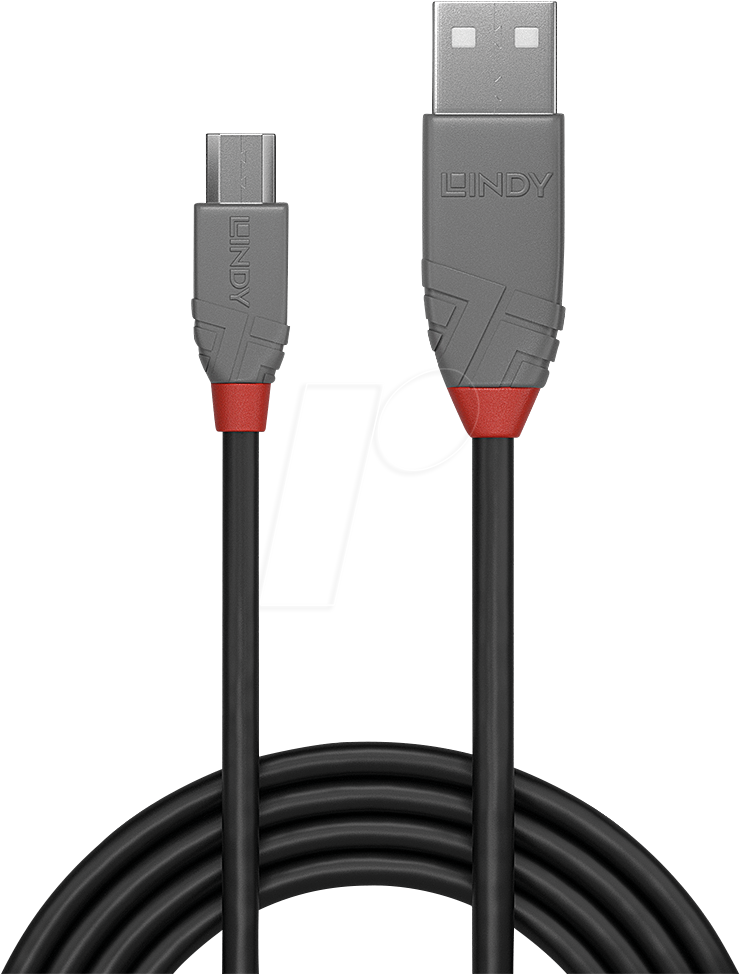
\includegraphics[width=3cm]{Images/BillofMaterials/USB}
	\caption{\textbf{USB}}
	\label{fig:USB}
\end{figure}

\section{Sticky Tape}

\textbf{tesa® WALLPAPER} is a thin but tear-resistant masking tape that has been specially developed for use on very sensitive surfaces such as paper wallpaper or fine plaster. The wallpaper tape is easy to apply, allows precise work with clean paint edges, and can be removed within seven days without leaving any residue. Since the masking tape is suitable for all types of paint, it is the ideal basis for renovation work where you want to protect sensitive surfaces indoors.

\subsection{Features}
\begin{itemize}[noitemsep]
	\item Specially designed for sensitive surfaces such as paper wallpaper.
	\item Masking tape can be removed without leaving any residue for up to seven days.
	\item Solvent-free and primarily made from renewable raw materials.
	\item Suitable for all types of paint.
\end{itemize}

\subsection{Dimensions}
\begin{itemize}[noitemsep]
	\item \textbf{Width:} 25 mm
	\item \textbf{Length:} 25 m
	\item \textbf{Quantity:} 1 Roll
\end{itemize}

\textbf{Metrics}
\begin{itemize}[noitemsep]
	\item \textbf{Length:} 25 m
	\item \textbf{Width:} 25 mm
\end{itemize}

\textbf{Other}
\begin{itemize}[noitemsep]
	\item \textbf{Specification:} For sensitive substrates
\end{itemize}

\textbf{Packaging}
\begin{itemize}[noitemsep]
	\item \textbf{Packaging:} 1 roll
\end{itemize}

\textbf{Manufacturer}
\begin{itemize}[noitemsep]
	\item \textbf{Manufacturer:} TESA
	\item \textbf{Manufacturer's Article Number:} 56260-00000-03
	\item \textbf{Tare:} 0.0787 kg
	\item \textbf{RoHS:} Compliant
	\item \textbf{EAN / GTIN:} 4042448149992
\end{itemize}


\begin{figure}[h!]\centering
	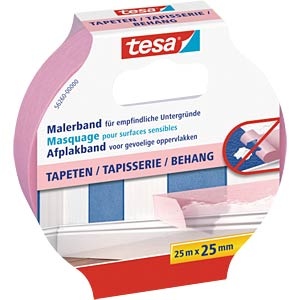
\includegraphics[width=3cm]{Images/BillofMaterials/Tape}
	\caption{\textbf{Tapes}}
	\label{fig:Tape}
\end{figure}

%%%%%%%%%%%%
%
% $Autor: Adhiraj, Sudheshna,Srikhant $
% $Datum: 2024-12-25 08:03:15Z $
% $Pfad: TemplateSensor $
% $Version: 4250 $
% !TeX spellcheck = en_GB/de_DE
% !TeX encoding = utf8
% !TeX root = filename 
% !TeX TXS-program:bibliography = txs:///biber
%
%%%%%%%%%%%%

% Structure
\chapter{Sensor/Actor}

\section{Accelerometer}

\subsection{Description}
The accelerometer enables significant motion detection (SMD), which recognizes large-scale movements. SMD can be used to activate specific device functions, such as waking the system from sleep mode or triggering predefined actions based on significant gestures.\cite{Zhou:2020}

The LSM9DS1 is a versatile and energy-efficient IMU with advanced sensing capabilities, supporting a range of applications where motion detection, orientation tracking, and gesture recognition are essential. Its compact design, low power consumption, and robust environmental tolerance make it a reliable choice for portable, battery-powered devices like the Magic Wand.\cite{Zhou:2020}
	
An \ac{imu} consists of three sensors that measure an object's orientation, position, vibration and movement in 3D space in real-time. These sensors are typically arranged in a pattern, including a tri-axial accelerometer, gyroscope, and magnetometer\cite{Ahmad:2013}. An accelerometer is used to measure the change in velocity of a moving or vibrating object\cite{Ahmad:2013}. Gyroscope measures the angular rotation\cite{Ahmad:2013}. A Magnetometer is used to measure yaw angle rotation, calibrating to the gyroscope data to improve the big drift issue\cite{Ahmad:2013}. 

The accelerometer functions by gauging the acceleration (Ax, Ay, Az), which denotes the rate of acceleration change over time. The acceleration values along each axis are conventionally expressed in units of meters per second squared $(m/s^2)$ \cite{Vernier:2023}. To illustrate, if the LSM9DS1 records an acceleration of 15 $m/s^2$ along the x-axis, this signifies that the object under observation is experiencing a velocity increment of 15 meters per second every second in the x-direction.
\subsection{Specific Sensors}
\textbf{Tilt Detection}
Using the accelerometer, the IMU can detect orientation changes with minimal power usage. Tilt detection is particularly useful for identifying subtle shifts in position, enhancing the responsiveness of gesture-based controls.\cite{Zhou:2020}

\textbf{Significant Motion Detection}
The accelerometer enables significant motion detection (SMD), which recognizes large-scale movements. SMD can be used to activate specific device functions, such as waking the system from sleep mode or triggering predefined actions based on significant gestures.\cite{Zhou:2020}

The LSM9DS1 is a versatile and energy-efficient IMU with advanced sensing capabilities, supporting a range of applications where motion detection, orientation tracking, and gesture recognition are essential. Its compact design, low power consumption, and robust environmental tolerance make it a reliable choice for portable, battery-powered devices like the Magic Wand.\cite{Zhou:2020}
	
An \ac{imu} consists of three sensors that measure an object's orientation, position, vibration and movement in 3D space in real-time. These sensors are typically arranged in a pattern, including a tri-axial accelerometer, gyroscope, and magnetometer\cite{Ahmad:2013}. An accelerometer is used to measure the change in velocity of a moving or vibrating object\cite{Ahmad:2013}. Gyroscope measures the angular rotation\cite{Ahmad:2013}. A Magnetometer is used to measure yaw angle rotation, calibrating to the gyroscope data to improve the big drift issue\cite{Ahmad:2013}. 

The accelerometer functions by gauging the acceleration (Ax, Ay, Az), which denotes the rate of acceleration change over time. The acceleration values along each axis are conventionally expressed in units of meters per second squared $(m/s^2)$ \cite{Vernier:2023}. To illustrate, if the LSM9DS1 records an acceleration of 15 $m/s^2$ along the x-axis, this signifies that the object under observation is experiencing a velocity increment of 15 meters per second every second in the x-direction.

\subsection{Specification}
\subsection{Library}
Details about libraries used to interface with accelerometers (e.g., Adafruit Sensor Library, Arduino libraries).
Installation process and setup.
Features provided by these libraries (e.g., data acquisition, filtering, scaling).
\begin{verbatim}
// Include the necessary libraries
#include <Wire.h>
#include <Adafruit_Sensor.h>
#include <Adafruit_LSM9DS1.h>
\end{verbatim}
\subsection{Functions}
\begin{verbatim}
// Check if acceleration data is available
if (IMU.accelerationAvailable()) {
	// Read the acceleration values
	IMU.readAcceleration(x, y, z);
	
	// Print the acceleration values
	Serial.print("AccX: ");
	Serial.print(x);
	Serial.print(", AccY: ");
	Serial.print(y);
	Serial.print(", AccZ: ");
	Serial.println(z);
}

\end{verbatim}
\subsection{Calibration}
Steps for calibrating an accelerometer:
\begin{itemize}
	\item Importance of calibration for accelerometer sensors.
	\item Methods for calibrating accelerometers (e.g., zeroing, scaling, temperature compensation).
	\item Tools and techniques for accelerometer calibration (e.g., software tools, calibration kits).
\end{itemize}

\subsection{Simple Code}
\begin{verbatim}
		#include <Wire.h>
		#include <Adafruit_Sensor.h>
		#include <Adafruit_LSM9DS1.h>

		// Create LSM9DS1 object
		Adafruit_LSM9DS1 lsm = Adafruit_LSM9DS1();

		void setup() {
		// Start the Serial Monitor
		Serial.begin(115200);

		// Initialize the LSM9DS1
		if (!lsm.begin()) {
			Serial.println("Failed to initialize LSM9DS1! Check wiring.");
			while (1);
		}

		// Set accelerometer range (default is ±2g)
		lsm.setupAccel(lsm.LSM9DS1_ACCELRANGE_2G);  
		// Options: 2G, 4G, 8G, 16G

		// Optional: Set accelerometer data rate (default is 119 Hz)
		lsm.setupAccelDataRate(lsm.LSM9DS1_ACCELDATARATE_119HZ);
		}

		void loop() {
		// Read accelerometer data
		sensors_event_t accelEvent;
		lsm.getEvent(&accelEvent, NULL, NULL);  
		// Get accelerometer event data only

		// Print accelerometer readings (in m/s²)
		Serial.print("Accel X: ");
		Serial.print(accelEvent.acceleration.x);
		Serial.print(" m/s², Y: ");
		Serial.print(accelEvent.acceleration.y);
		Serial.print(" m/s², Z: ");
		Serial.print(accelEvent.acceleration.z);
		Serial.println(" m/s²");

		// Delay to make output more readable
		delay(100);
		}

\end{verbatim}
\subsection{Applications}
Practical uses of accelerometers:
\begin{itemize}
	\item In smartphones (e.g., screen orientation, motion detection).
	\item Automotive industry (e.g., airbag deployment, stability control).
	\item Robotics (e.g., navigation, balance).
	\item Wearable devices and fitness trackers.
	\item Industrial applications (e.g., vibration monitoring, machine diagnostics).
\end{itemize}
\subsection{Tests}
Techniques to test an accelerometer’s functionality:
This is the C++ code for testing the accelerometer on the Arduino Nano 33 BLE Sense using the \texttt{Adafruit\_LSM9DS1} library. 

\begin{figure}[h!]
	\centering
	\begin{lstlisting}[style=pythonstyle ,language=C++, caption={Testing the accelerometer}, label={lst:arduino_accelerometer}]
		#include <Wire.h>
		#include <Adafruit_Sensor.h>
		#include <Adafruit_LSM9DS1.h>
		
		// Create an instance of the LSM9DS1 sensor
		Adafruit_LSM9DS1 lsm = Adafruit_LSM9DS1();
		
		void setup() {
			// Start serial communication
			Serial.begin(115200);
			
			// Initialize the LSM9DS1 sensor
			if (!lsm.begin()) {
				Serial.println("Could not find a valid LSM9DS1 sensor, check wiring!");
				while (1);
			}
			
			Serial.println("LSM9DS1 test initialized.");
		}
		
		void loop() {
			// Read accelerometer data
			sensors_event_t event;
			lsm.getEvent(&event);
			
			// Print accelerometer values
			Serial.print("X: ");
			Serial.print(event.acceleration.x);
			Serial.print(" Y: ");
			Serial.print(event.acceleration.y);
			Serial.print(" Z: ");
			Serial.println(event.acceleration.z);
			
			// Delay before the next reading
			delay(1000);
		}
	\end{lstlisting}
	\caption{C++ code for testing the accelerometer on the Arduino Nano 33 BLE Sense.}
	\label{lst:cpp_code}
\end{figure}

This is the Python code for reading the accelerometer data from the Arduino via serial communication. The \texttt{pyserial} library is required for this script.

\begin{figure}[h!]
	\centering
	\begin{lstlisting}[style=pythonstyle ,language=python, caption={Accelerometer testing in pyserial}, label={lst:arduino_accelerometer}]
		import serial
		import time
		
		# Replace with the correct port for your system (e.g., 'COM3' on Windows or '/dev/ttyACM0' on Linux)
		arduino_port = '/dev/ttyACM0'  
		baud_rate = 115200
		
		# Establish connection to the Arduino
		arduino = serial.Serial(arduino_port, baud_rate, timeout=1)
		time.sleep(2)  # Wait for Arduino to initialize
		
		# Function to read accelerometer data from the Arduino
		def read_accelerometer():
		while True:
		line = arduino.readline().decode('utf-8').strip()
		if line:
		print(line)
		
		# Start reading accelerometer data
		read_accelerometer()
	\end{lstlisting}
	\caption{Python code for reading accelerometer data from the Arduino Nano 33 BLE Sense.}
	\label{lst:python_code}
\end{figure}

\subsection{Further Readings}

\section{Gyroscope}
\subsection{Description}
The STMicroelectronics LSM9DS1 gyroscope is a precision instrument for measuring angular velocity around the x, y, and z axes. With adaptable measurement ranges of ±245, ±500, and ±2000 degrees per second (dps), the gyroscope is highly versatile for various applications such as inertial navigation, robotics, and drone stabilization.\cite{St:2024}
Key Features:
\begin{itemize}
\item Sampling Rates: The gyroscope offers adjustable sampling rates, allowing it to operate at frequencies of 14.9 Hz, 59.5 Hz, 119 Hz, 238 Hz, 476 Hz, or 952 Hz.\cite{St:2024} This flexibility ensures compatibility with a broad range of motion measurement requirements.

\item Voltage and Power Consumption: The gyroscope operates within a voltage range of 1.71 V to 3.6 V, making it suitable for different system configurations.\cite{St:2024} Its low power consumption—between 1 mA to 2 mA—enhances its suitability for portable, battery-operated devices.\cite{St:2024}

\item Compact Design: The LSM9DS1 integrates seamlessly into compact systems, offering engineers and designers a robust yet space-efficient solution.\cite{Maker:2024}

\item Operation Principle: The gyroscope operates based on Coriolis acceleration, a phenomenon observed when a vibrating object moves in a rotating reference frame. Piezoelectric crystals are used to detect changes in angular velocity by converting inertial forces into electrical signals.

\item Applications: The LSM9DS1 gyroscope is designed for:
\end{itemize}
Inertial Measurement Units (IMUs): Combined with accelerometers and magnetometers, it forms a 9-DOF motion tracking system.\cite{Ahmad:2013}
Drone Stabilization: Essential for real-time attitude adjustments.\cite{Ahmad:2013}
Navigation Systems: Key in applications like gyrocompasses or attitude heading reference systems.\cite{Ahmad:2013}

$$ \text{Angular velocity} = \left(\frac{\text{Gyroscope axis raw data}}{65536} \times \text{full scale Gyroscope range}\right) \frac{\circ}{\text{s}} $$

For example, if the gyroscope's raw data along the X axis is 16384 and the range is ±250°/s, the calculation for angular velocity along the X axis would be:

$$ \text{Angular velocity along the X axis} = \left(\frac{16384}{65536} \times 500\right) \frac{\circ}{\text{s}} = 125 \frac{\circ}{\text{s}} $$


\begin{figure}[H]\centering
	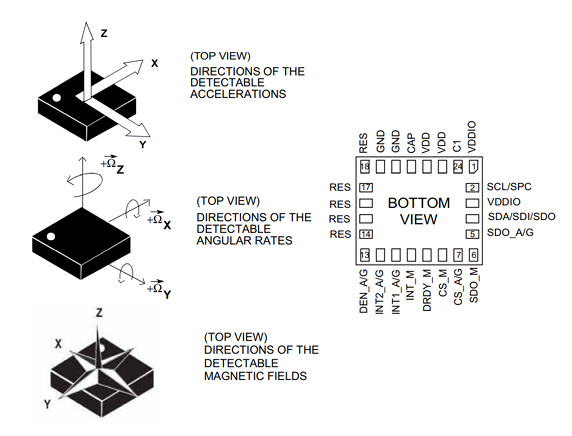
\includegraphics[width=0.8\textwidth]{Images/Sensor Actor/Gyroscope} 
	\caption{\textbf{Gyroscope}}
	\label{fig:Pin_assignment_of_Arduino_Nano_33_BLE_Sense} 
\end{figure}
\begin{figure}[H]\centering
	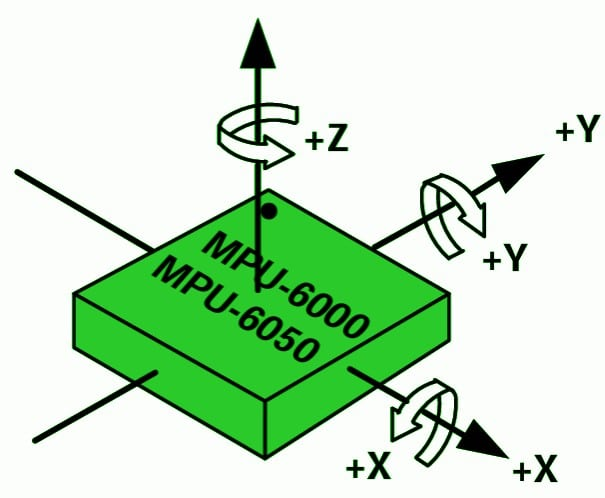
\includegraphics[width=0.8\textwidth]{Images/Sensor Actor/orientation_axes} 
	\caption{\textbf{Orientation Axes of Gyroscope}}
	\label{fig:Pin_assignment_of_Arduino_Nano_33_BLE_Sense} 
\end{figure}
\subsection{Specification}

	\textbf{Gyroscope Specifications of MPU6050:}\newline
	\begin{tabular}{|l|l|l|}
		\hline
		Full scale range & FS\_SEL & Range \\ \hline
		& 0 & ±250°/s \\ \hline
		& 1 & ±500°/s \\ \hline
		& 2 & ±1000°/s \\ \hline
		& 3 & ±2000°/s \\ \hline
		Sensitivity Scale Factor Tolerance & & ±3\% \\ \hline
		Gyroscope start-up time && 30 ms \\ \hline
		Output data rate & & 4 to 8000 Hz \\ \hline
	\end{tabular}

\subsection{Library}

{Description}
To meet the project's needs, three essential libraries must be integrated, each serving a specific purpose that ensures smooth operation and functionality of the system. Here's a breakdown of each library’s role:

\textbf{1. Wire.h:}
   This is an Arduino standard library used for I2C communication, a protocol that allows devices to communicate with each other using only two wires, reducing the complexity of wiring in systems that need to connect multiple devices. I2C is widely used for connecting sensors, displays, and other peripherals to a microcontroller. The `Wire.h` library simplifies interactions with I2C devices by handling the low-level details of communication. Developers can initialize the I2C bus, send and receive data, and manage multiple I2C devices on the same bus seamlessly. This is crucial for systems that need to manage several sensors or external modules, as it facilitates smooth and efficient data transfer.\cite{Passaro:2017}

\textbf{2. Kalman.h:}
   The Kalman filter is an advanced mathematical algorithm used to process noisy sensor data and provide more accurate estimates of a system’s state. The `Kalman.h` library allows developers to easily implement this filter into Arduino-based projects. It is particularly useful in applications where precise data is essential, such as robotics, control systems, and navigation. By filtering out noise and accounting for uncertainties in sensor readings, the Kalman filter improves the accuracy of measurements like position, velocity, and orientation, which are crucial in motion tracking, sensor fusion, or stabilizing systems like drones and robots.\cite{Passaro:2017}

\textbf{3. Arduino\_LSM9DS1.h:}
   This library is specifically designed to interface with the LSM9DS1 IMU (Inertial Measurement Unit) sensor, developed by STMicroelectronics. The LSM9DS1 combines three essential motion sensors in one package: an accelerometer, a gyroscope, and a magnetometer. The `Arduino\_LSM9DS1.h` library allows developers to easily access data from these sensors, such as acceleration, angular velocity, and magnetic field strength. Additionally, the library offers functions to configure sensor parameters like measurement ranges, sampling rates, and operating modes, enabling customization based on the needs of the application. This is particularly useful in systems that rely on accurate motion tracking or orientation sensing.\cite{Passaro:2017}

Together, these libraries enable the integration of multiple sensors into a cohesive system, facilitating communication, data processing, and precise motion measurement.

\subsection{Installation}
\begin{figure}[H]\centering
	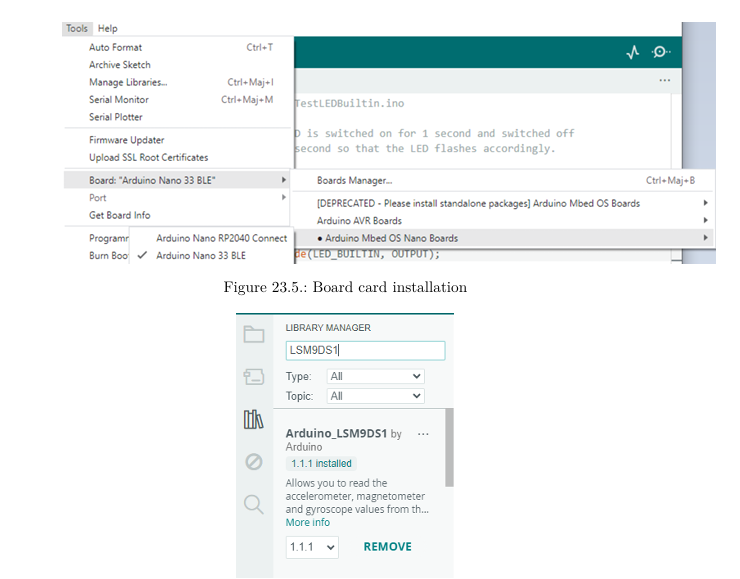
\includegraphics[width=0.8\textwidth]{Images/Sensor Actor/Installation} 
	\caption{\textbf{Installation of Libraries}}
	\label{fig:Pin_assignment_of_Arduino_Nano_33_BLE_Sense} 
\end{figure}
\begin{figure}[H]\centering
	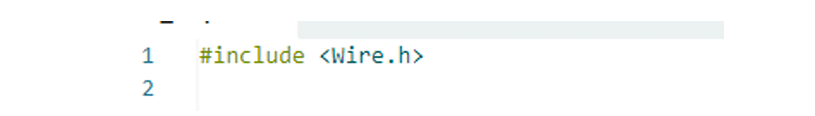
\includegraphics[width=0.8\textwidth]{Images/Sensor Actor/Installation_of_wire} 
	\caption{\textbf{Installation of wire.h}}
	\label{fig:Pin_assignment_of_Arduino_Nano_33_BLE_Sense} 
\end{figure}
\subsection{Functions}
The LSM9DS1 library for the Arduino Nano 33 BLE Sense provides a set of functions to interact with the LSM9DS1 IMU (Inertial Measurement Unit) sensor. The functions available depend on the communication protocol being used, either I2C or SPI.\cite{Passaro:2017}



\textbf{Function IMU.readGyroscope()}
The function IMU.readGyroscope() is used to retrieve data from an Inertial Measurement Unit's (IMU) gyroscope. It returns the angular velocity in degrees per second (dps), providing information about the rotational movement detected by the IMU. This data is crucial for applications like robotics, motion tracking, and navigation systems, where precise orientation control and stabilization are required.
The function typically returns x, y, and z values, representing the angular velocity along each of the three axes (x, y, and z). These values are floating-point numbers that describe the rotational velocity along each axis, enabling detailed tracking of changes in orientation. By regularly calling this function and analyzing the data over time, it becomes possible to monitor and respond to rotational movements accurately.
For example, in robotics, these readings can be used to adjust a robot’s position or orientation in real-time, while in drones, they assist with stabilization during flight.
\begin{code}[h!]
	\begin{Arduino}
  // Declare variables to store gyroscope data
  float x, y, z;
  
  // Check if gyroscope data is available
  if (IMU.gyroscopeAvailable()) {  
  	// Read the gyroscope data into variables x, y, z
  	IMU.readGyroscope(x, y, z);   
  	
  	// Print the x-axis angular velocity
  	Serial.print(x);               
  	
  	// Print a tab space for separation
  	Serial.print('\t');            
  	
  	// Print the y-axis angular velocity
  	Serial.print(y);               
  	
  	// Print another tab space for separation
  	Serial.print('\t');            
  	
  	// Print the z-axis angular velocity and move to the next line
  	Serial.println(z);             
  }
  
\end{Arduino}
\caption{Sample Code of IMU.readGyroscope()}\label{code:IMU.readGyroscope()}
\end{code}\newline
\textbf{Function IMU.gyroscopeAvailable()}
The function IMU.gyroscopeAvailable() is used to check whether new gyroscope data is available from the IMU. It returns a value of 1 if new data is ready to be retrieved, and 0 if no new data is available. This function is particularly useful in real-time applications, such as drone stabilization, virtual reality systems, or inertial navigation, where the system must determine whether to wait for updated gyroscope data or proceed with processing the available information.

For example, in a drone application, when the function returns 1, the system knows that new gyroscope data is available, and it can proceed to retrieve and use this information to adjust the drone's orientation or stabilize its motion. Conversely, a return value of 0 means that no new data has been received, prompting the system to wait until new data is available before continuing the process.

In the provided code example:\newline
\begin{code}[h!]
	\begin{Arduino}
	// Declare variables to store gyroscope data
	float x, y, z;
	
	// Check if gyroscope data is available
	if (IMU.gyroscopeAvailable()) {
		// Read the gyroscope data into variables x, y, z
		IMU.readGyroscope(x, y, z);
		
		// Print the x-axis angular velocity
		Serial.print(x);
		
		// Print a tab space for separation
		Serial.print('\t');
		
		// Print the y-axis angular velocity
		Serial.print(y);
		
		// Print another tab space for separation
		Serial.print('\t');
		
		// Print the z-axis angular velocity and move to the next line
		Serial.println(z);
	}
	
	\end{Arduino}
\caption{Sample Code of IMU.gyroscopeAvailable()}\label{code:IMU.gyroscopeAvailable()}
\end{code}
The program checks if new gyroscope data is available. If it is, the data is read and output to the serial monitor, showing the angular velocity along the x, y, and z axes.
This function is integral for applications that require continuous monitoring of rotational movement, ensuring that the system can react promptly to changes in orientation.

\textbf{Function IMU.gyroscopeSampleRate()}
The function IMU.gyroscopeSampleRate() is used to retrieve the rate at which the gyroscope integrated into the Inertial Measurement Unit (IMU) collects samples, typically expressed in Hertz (Hz). This sample rate indicates how frequently the gyroscope measures angular velocity, providing insights into its operational efficiency and performance.

\textbf{Sample Rate:} It is the frequency at which the gyroscope takes measurements. For example, a sample rate of 100 Hz means the gyroscope takes 100 readings per second.
\newline
\begin{code}[h!]
	\begin{Arduino}
	// Print the gyroscope sample rate
	Serial.print("Gyroscope sample rate= ");
	Serial.print(IMU.gyroscopeSampleRate());  // Print the gyroscope sample rate
	Serial.println("Hz");
	Serial.println();  // Print a blank line for separation
	
	// Print a label for angular speed in degrees/second
	Serial.println("Angular speed in degrees/second");
	
	// Print the axis labels with tab separation
	Serial.println("X\tY\tZ");
	
	\end{Arduino}
\caption{Sample Code of IMU.gyroscopeSampleRate()}\label{code:IMU.gyroscopeSampleRate()}
\end{code}	
\textbf{Function Breakdown:}
IMU.gyroscopeSampleRate(): This function returns the sample rate of the gyroscope in Hertz (Hz).
The Serial.print() functions then display the sample rate and additional information about the angular speed readings in degrees per second for the X, Y, and Z axes.

This function is especially useful in applications that require accurate and efficient motion tracking, such as drone stabilization, robotics, or virtual reality systems. Knowing the sample rate helps determine how often new data is available, which influences the system's ability to respond to changes in rotational movement.


\subsection{Calibration}
There are various methods to calibrate the sensors involved. It is necessary to know whether the sensor is balanced since the time between each calibration needs to be explicitly defined. Regular calibration should be done, especially when strange outputs are noticed. 

	Some methods of calibration are briefed below:
\begin{itemize}
\item
\textbf{Low and high limit method}\newline The low and high limit method involves recording minimum and maximum values on all three axes using a simple scratch to determine their absolute values. The sensor undergoes circular rotations along each axis multiple times. The centre point is then identified between these extremes.\cite{Gyroplace:2023}
Increasing the number of rotations enhances the likelihood of capturing the absolute peak. The center point will be close to zero if the sensor exhibits no offset. However, slight variations may indicate a hard iron offset attributed to distortion caused by the Earth’s magnetic field.\cite{Gyroplace:2023}
This method assumes minimal soft iron distortion, evident from the rounded outlines in the graph.\cite{Gyroplace:2023}
It is important to note that this method necessitates capturing values each time to prevent performance degradation due to component drift and aging sensors. For devices relying on primary batteries, calibration becomes essential after each battery change, as the battery inevitably serves as the main source of magnetic disturbance, and new batteries may behave differently from their predecessors.\cite{Gyroplace:2023}

\item
\textbf{Scale Factor and Non-Orthogonal Calibration}\newline With given initial attitude derived from alignment procedure, the gyroscope measurement can be integrated to calculate the orientation information through Strapdown inertial navigation algorithm. However, the computed attitude will drift over time and the error is gradually accumulated because of the sensor error. In stationary or low dynamic condition, the accelerometer output can be used to estimate the orientation relative to horizontal plane (i.e., pitch and roll).\cite{Gyroplace:2023} The attitude derived from accelerometer output is independent in different time epochs and not affected by accumulated error. Hence, based on the different sensors’ complimentary error propagation characteristics, we can make use of the accelerometer-derived attitude as reference signal to evaluate the attitude error introduced during integration process, and consequently determine the gyroscope error.\cite{Gyroplace:2023}
\end{itemize}
During the calibration process, the IMU is handheld by user and rotated along its axes slowly to avoid introducing external acceleration. The IMU orientation keeps varying during this procedure and the attitudes derived from different inertial sensors are compared to amend the attitude error and determine the sensor errors. A Kalman filter is designed to estimate the scale factor and non-orthogonal errors of gyroscope. The attitude error propagation equation, which includes sensor error, is utilized as the system dynamic model. The relationship between the accelerometer output and attitude error is modeled as the measurement equation.\cite{Gyroplace:2023}
\newline
\subsection{Simple Code}

Example IMU: Accelerometer and Gyroscope
\begin{code}
	\begin{Arduino}
		#include <Arduino_LSM9DS1.h>

		void setup() {
		Serial.begin(9600);

		// Initialize the IMU
		if (!IMU.begin()) {
			Serial.println("Failed to initialize IMU!");
			while (1); // Stop execution if initialization fails
		}
		}
		void loop() {
		float x, y, z;

		// Check if new acceleration data is available
		if (IMU.accelerationAvailable()) {
			IMU.readAcceleration(x, y, z);
			Serial.print("AccX: ");
			Serial.print(x);
			Serial.print(", AccY: ");
			Serial.print(y);
			Serial.print(", AccZ: ");
			Serial.println(z);
		}
		// Check if new gyroscope data is available
		if (IMU.gyroscopeAvailable()) {
			IMU.readGyroscope(x, y, z);
			Serial.print("GyroX: ");
			Serial.print(x);
			Serial.print(", GyroY: ");
			Serial.print(y);
			Serial.print(", GyroZ: ");
			Serial.println(z);
		}
		delay(1000); // Wait for 1 second before reading again
		}
	\end{Arduino}
	\caption{Example code for reading accelerometer and gyroscope data from the LSM9DS1 IMU}\label{code:IMU-example}
\end{code}

\subsection{Simple Application}
Gyroscopes in IMUs are essential for detecting and maintaining orientation and rotational motion in a wide range of devices:

\begin{itemize}
	\item \textbf{Smartphones/Tablets}: They enable features like screen auto-rotation and motion controls for gaming and virtual reality (VR).\cite{Passaro:2017}
	\item \textbf{Drones}: Gyroscopes stabilize flight by measuring angular velocity, allowing the drone to correct tilt and maintain stable orientation.\cite{Passaro:2017}
	\item \textbf{Robotics}: In robots, gyroscopes assist in balancing and navigation by tracking rotational movements, ensuring accurate motion control.\cite{Passaro:2017}
	\item \textbf{VR/AR}: In virtual and augmented reality systems, gyroscopes track head movement to provide an immersive experience by adjusting visuals based on real-time orientation.\cite{Passaro:2017}
\end{itemize}

\subsection{Testing}

The following code reads the gyroscope data (X, Y, and Z axes) from the LSM9DS1 sensor on the Arduino Nano 33 BLE Sense and sends it to the Serial Monitor.

\begin{lstlisting}[style=pythonstyle ,language=C++, caption={Arduino Code to Test the Gyroscope}, label={lst:arduino_gyroscope}]
	#include <Wire.h>
	#include <Adafruit_Sensor.h>
	#include <Adafruit_LSM9DS1.h>
	
	// Create an instance of the LSM9DS1 sensor
	Adafruit_LSM9DS1 lsm = Adafruit_LSM9DS1();
	
	void setup() {
		// Start serial communication
		Serial.begin(115200);
		
		// Initialize the LSM9DS1 sensor
		if (!lsm.begin()) {
			Serial.println("Could not find a valid LSM9DS1 sensor, check wiring!");
			while (1);
		}
		
		Serial.println("LSM9DS1 Gyroscope test initialized.");
	}
	
	void loop() {
		// Read gyroscope data
		sensors_event_t event;
		lsm.getEvent(&event);
		
		// Print gyroscope values
		Serial.print("Gyroscope X: ");
		Serial.print(event.gyro.x);
		Serial.print(" Y: ");
		Serial.print(event.gyro.y);
		Serial.print(" Z: ");
		Serial.println(event.gyro.z);
		
		// Delay before the next reading
		delay(1000);
	}
\end{lstlisting}

\subsection{Python Code}
The following Python script reads the gyroscope data sent by the Arduino and prints the values. Ensure you have the \texttt{pyserial} library installed.

\textbf{Install the \texttt{pyserial} library}:
\begin{lstlisting}[style=bashstyle ,language=bash, caption={Installing pyserial}, label={lst:install_pyserial}]
	pip install pyserial
\end{lstlisting}

\textbf{Python Code}:
\begin{lstlisting}[language=Python ,style=pythonstyle ,caption={Python Code to Read and Test Gyroscope Data}, label={lst:python_gyroscope}]
	import serial
	import time
	
	# Set up the serial connection (replace with your actual port)
	ser = serial.Serial('COM3', 115200)  # For Windows, replace COM3 with your port, for Mac/Linux, it may be /dev/ttyACM0 or /dev/ttyUSB0
	
	# Allow some time for the Arduino to reset and start transmitting data
	time.sleep(2)
	
	# Loop to continuously read gyroscope data
	while True:
	try:
	# Read a line of data from Arduino
	line = ser.readline().decode('utf-8').strip()
	
	# Only print the line if it contains the "Gyroscope" data
	if 'Gyroscope' in line:
	print(line)
	
	# Delay before the next reading
	time.sleep(1)
	
	except KeyboardInterrupt:
	print("Exiting...")
	break
	
	# Close the serial connection when done
	ser.close()
\end{lstlisting}

\subsection{Further Readings}
Schanda, Janos: Colorimetry: Understanding the CIE System.Wiley, 2007.[\cite{Schanda:2007}]
Lukac, Rastislav and Plataniotis, Konstantinos N.: Color Image Processing:
Methods and Applications.CTC Press,2018.[\cite{Lukac:2018}]

\section{Magnetometer}
\begin{figure}[h!]\centering
	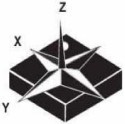
\includegraphics[width=6cm]{Images/HardwareDescription/MagnetometerDirection}
	\caption{\textbf{Magnetometer Directions}}
	\label{fig:Magnetometer}
	\cite{Stm:2015}
\end{figure}
\subsection{Description}
In the context of a magnetometer, the x, y, and z axes (Mx, My, Mz) typically delineate the three-dimensional space in which the magnetic field is being assessed. The x-axis typically corresponds to the horizontal component of the magnetic field, the y-axis signifies the vertical component, and the z-axis reflects the magnetic field strength \cite{Kostiainen:2023}. This three-dimensional measurement provides a comprehensive understanding of the magnetic field in the surrounding space.
A magnetometer is a sensor that measures the strength and direction of a magnetic field. It is commonly used to detect the Earth's magnetic field for navigation purposes, detect magnetic anomalies, or determine heading in devices like smartphones, drones, and robotics. Magnetometers are fundamental in compasses, GPS systems, and geological exploration (Ripka, 2001).
\subsection{Specific Sensors}
There are various types of magnetometers available, differing in precision, range, and applications. Here are some popular ones:
\begin{itemize}
	\item HMC5883L: A widely used 3-axis digital magnetometer that provides low-cost magnetic field measurement \cite{Honeywell:2012}.
	\item LSM303DLHC: Combines an accelerometer and magnetometer, enabling tilt-compensated compass applications \cite{Adafruit:2021a}.
	\item AK8963: A 3-axis magnetometer typically used with IMUs like the MPU9250 for high accuracy \cite{AsahiKasei:2014}.
	\item MAG3110: A small, low-power 3-axis magnetometer for embedded systems \cite{NXP:2013}.
\end{itemize}
\subsection{Specification}

General magnetometer specifications include:
\begin{itemize}
	\item 3D digital magnetic sensor: Detects magnetic fields with a full scale of ±4/±8/±12/±16 gauss.
	\item Axes: Single-axis or 3-axis (most modern sensors are 3-axis).
	\item Sensitivity: Ability to detect weak magnetic fields (e.g., microteslas, nanoteslas).
	\item Range: Typically between ±8 to ±100 microteslas.
	\item Resolution: The smallest change in the magnetic field that the sensor can detect.
	\item Power Consumption: Important for portable systems.
\item Interface: I2C, SPI, or analog output.
\end{itemize}
\subsection{Library}
Libraries simplify interfacing with magnetometer sensors, converting raw data into readable formats. Below are some libraries:

Arduino:
\begin{itemize}
	\item HMC5883L: Adafruit\_HMC5883\_Unified.h (Adafruit, 2021b).
	\item LSM303: Adafruit\_LSM303DLHC.h (Adafruit, 2021a).
\end{itemize}
Python:
\begin{itemize}
	\item Use smbus or CircuitPython libraries for I2C sensors \cite{Adafruit:2020}.
	\item Example for Raspberry Pi: hmc5883l Python library \cite{Hollingworth:2019}.
\end{itemize}
To install the library for Arduino:

\begin{verbatim}
// Include the necessary libraries
#include <Adafruit_Sensor.h>
#include <Adafruit_HMC5883_U.h>
\end{verbatim}

\subsection{Calibration}
Basic calibration steps:
\begin{itemize}
	\item Rotate the sensor in all directions.
	\item Plot the data to ensure it forms a circle.
	\item Apply corrections for centering the data.
\end{itemize}
\subsection{Simple Code}
\begin{code}[h!]
	\begin{Arduino}
	// Include the necessary libraries
	#include <Wire.h>
	#include <Adafruit_Sensor.h>
	#include <Adafruit_HMC5883_U.h>
	// Create an HMC5883 magnetometer object with a unique ID
	Adafruit_HMC5883_Unified mag = Adafruit_HMC5883_Unified(12345);
	// Setup function
	void setup(void) {
		// Start serial communication at 9600 baud rate
		Serial.begin(9600);
		// Initialize the magnetometer
		if (!mag.begin()) {
			Serial.println("No HMC5883L detected ... Check your wiring!");
			while (1);  // Halt the program if the sensor is not detected
		}
		
		// Set the magnetometer gain
		mag.setMagGain(HMC5883_MAGGAIN_1_3);
	}
	// Loop function
	void loop(void) {
		// Declare a variable to store magnetometer data
		sensors_event_t event;
		// Get the magnetometer event data
		mag.getEvent(&event);
		// Calculate the heading angle in radians
		float heading = atan2(event.magnetic.y, event.magnetic.x);
		if (heading < 0) heading += 2 * PI;
		// Convert the heading from radians to degrees
		float headingDegrees = heading * 180 / M_PI;
		// Print the heading in degrees
		Serial.println(headingDegrees);
		// Delay for 500ms before the next reading
		delay(500);
	}
	
	\end{Arduino}
	\caption{Example code for reading magnetometer data}\label{code:magnetometer-example}
\end{code}
\subsection{Applications}
Magnetometers have diverse applications, including:
\begin{itemize}
	\item Navigation: Electronic compasses in GPS, drones, and aircraft \cite{Sherwood:2013}.
	\item Robotics: Precise heading information for autonomous systems \cite{IEEE:2020}.
	\item Consumer Devices: Smartphones, wearables for direction detection \cite{AsahiKasei:2014}.
	\item Geological Exploration: Detect magnetic anomalies for mineral exploration \cite{Hansen:2017}.
	\item Space Exploration: Magnetic field mapping on planets.
	\item Security: Detection of ferromagnetic objects in metal detectors \cite{Williams:2015}.
\end{itemize}
\subsection{Tests}

The following C++ code reads and prints the magnetometer data (X, Y, Z values) from the LSM9DS1 sensor connected to the Arduino Nano 33 BLE Sense.

\begin{lstlisting}[caption={C++ Code for Arduino to Read Magnetometer Data}, label={lst:cpp_magnetometer}, style=pythonstyle]
	#include <Wire.h>
	#include <Adafruit_Sensor.h>
	#include <Adafruit_LSM9DS1.h>
	
	// Create an instance of the LSM9DS1 sensor
	Adafruit_LSM9DS1 lsm = Adafruit_LSM9DS1();
	
	void setup() {
		// Start serial communication
		Serial.begin(115200);
		
		// Initialize the LSM9DS1 sensor
		if (!lsm.begin()) {
			Serial.println("Could not find a valid LSM9DS1 sensor, check wiring!");
			while (1);
		}
		
		Serial.println("LSM9DS1 test initialized.");
	}
	
	void loop() {
		// Read magnetometer data
		sensors_event_t event;
		lsm.getEvent(&event, Adafruit_LSM9DS1::MAGNETOMETER);
		
		// Print magnetometer values
		Serial.print("Mag X: ");
		Serial.print(event.magnetic.x);
		Serial.print(" Y: ");
		Serial.print(event.magnetic.y);
		Serial.print(" Z: ");
		Serial.println(event.magnetic.z);
		
		// Delay before the next reading
		delay(1000);
	}
\end{lstlisting}

\newpage

This Python code reads the magnetometer data from the Arduino via serial communication.

\begin{lstlisting}[style=pythonstyle, caption={Python Code to Read Magnetometer Data via Serial}, label={lst:python_magnetometer}]
	import serial
	import time
	
	# Replace with the correct port for your system (e.g., 'COM3' on Windows or '/dev/ttyACM0' on Linux)
	arduino_port = '/dev/ttyACM0'  
	baud_rate = 115200
	
	# Establish connection to the Arduino
	arduino = serial.Serial(arduino_port, baud_rate, timeout=1)
	time.sleep(2)  # Wait for Arduino to initialize
	
	# Function to read magnetometer data from the Arduino
	def read_magnetometer():
	while True:
	line = arduino.readline().decode('utf-8').strip()
	if line:
	print(line)
	
	# Start reading magnetometer data
	read_magnetometer()
\end{lstlisting}

\subsection{Further Readings}
For more information, refer to:

Datasheets: Sensor-specific datasheets (e.g., HMC5883L, LSM303).
Books:
\begin{itemize}
	\item Ripka, A. (2001) Introduction to Magnetometers. New York: Wiley.
	\item Sherwood, T. (2013) Magnetic Sensors in Navigation Systems. Berlin: Springer.
\end{itemize}
Online Resources:
\begin{itemize}
	\item Adafruit tutorials on magnetometers \cite{Adafruit:2021a}.
	\item Research papers on magnetic anomaly detection \cite{Hansen:2017}.
\end{itemize}









%%%%%%%%%%%%
%
% $Autor: Sudeshna $
% $Datum: 2019-03-05 08:03:15Z $
% $Pfad: TemplateSensor $
% $Version: 4250 $
% !TeX spellcheck = en_GB/de_DE
% !TeX encoding = utf8
% !TeX root = filename 
% !TeX TXS-program:bibliography = txs:///biber
%
%%%%%%%%%%%%

% Structure
\chapter{Domain System/Complete System}
\section{Description}
	The \texttt{Arduino Nano 33 BLE Sense} is a compact and low-power board ideal for IoT and AI applications, especially when space is a constraint. Its small size (\(45mm \times 18mm\)) and efficient power usage make it perfect for projects that require long battery life, operating at \(3.3V\). This board comes with a variety of embedded sensors, making it versatile for a range of applications.\cite{Gyroplace:2023} Below is a brief summary of the features on the board:
	
	\begin{itemize}
		\item \textbf{LEDs}: The board features three different LEDs for various purposes:
		\begin{itemize}
			\item \textbf{RGB Programmable LED}: Allows you to program different colors and effects for visual feedback.
			\item \textbf{Built-in Orange Programmable LED}: Can be used for status indication or customized signals.
			\item \textbf{Power LED}: Indicates that the board is powered on.
		\end{itemize}
		\item \textbf{Processor}: The board is powered by the \texttt{nRF52840} processor, a 32-bit ARM® Cortex™-M4 CPU running at 64 MHz, which is more powerful than many other Arduino boards, allowing it to handle more complex computations or real-time data processing.
		
		\item \textbf{USB-C Port}: The \texttt{Arduino Nano 33 BLE Sense} features a \textbf{USB-C port} for power and data transfer. This modern, reversible connector provides a reliable connection for both programming the board and powering it.
		
		\item \textbf{Power Button}: The board includes a \textbf{power button}, allowing you to manually power on or off the device without needing to disconnect it from the power source. This is useful for battery-powered projects, where conserving power or resetting the device is necessary.
	\end{itemize}
	
	The \texttt{Arduino Nano 33 BLE Sense} is ideal for low-power, compact devices that require real-time environmental sensing, motion tracking, or interactive capabilities, all within a small, portable form factor.\cite{Passaro:2017}
	

\section{Design}

\begin{figure}[H]\centering
	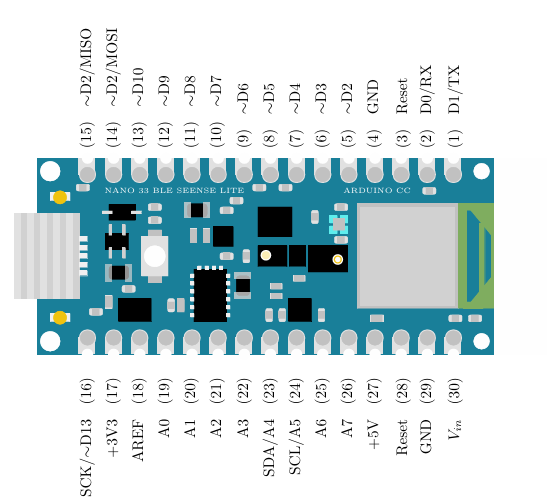
\includegraphics[width=0.8\textwidth]{Images/Sensor Actor/Pin_Assignment_of_Ardruino33BLEsense} 
	\caption{\textbf{Pin Assignment of Arduino Nano 33 BLE Sense}}
	\label{fig:Pin_assignment_of_Arduino_Nano_33_BLE_Sense} 
\end{figure}
\begin{figure}[H]\centering
	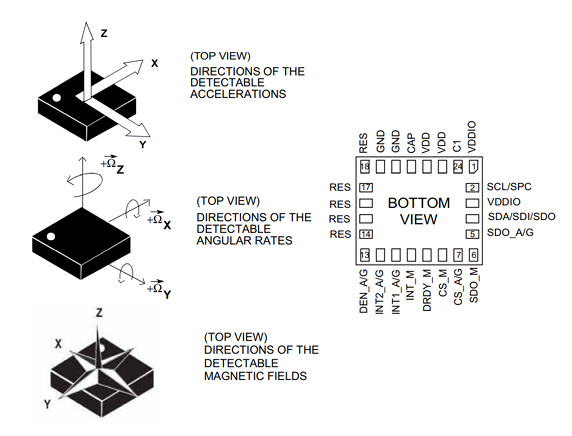
\includegraphics[width=0.8\textwidth]{Images/Sensor Actor/pin_connection_lsm9ds1} 
	\caption{\textbf{Pin Assignment of LSM9DS1}}
	\label{fig:Pin_assignment_of_Arduino_Nano_33_BLE_Sense} 
\end{figure}
\begin{figure}[H]\centering
	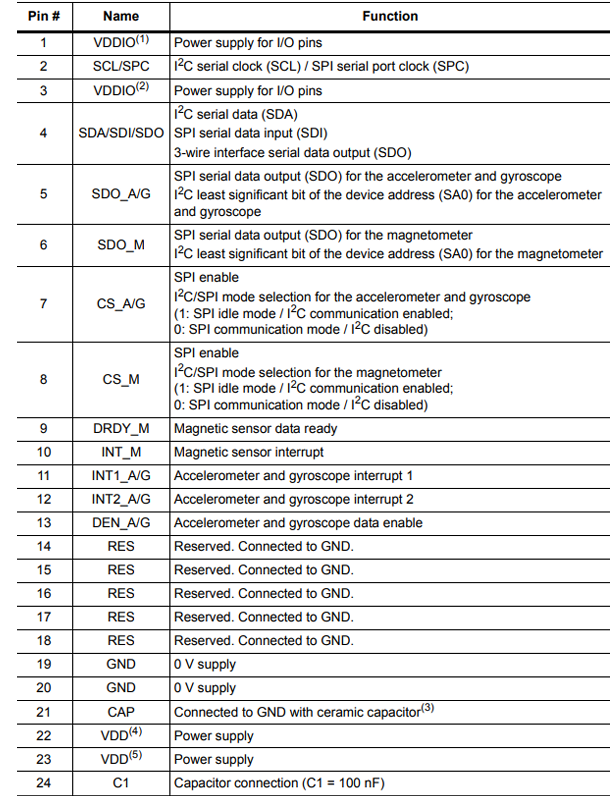
\includegraphics[width=0.8\textwidth]{Images/Sensor Actor/pin_description_lsm9ds1} 
	\caption{\textbf{Pin Description of LSM9DS1}}
	\label{fig:Pin_assignment_of_Arduino_Nano_33_BLE_Sense} 
\end{figure}
\section{Hardware Interface}

	The Arduino Nano 33 BLE Sense is a small and powerful development board featuring various hardware interfaces for communication, control, and interaction. The following sections describe the available interfaces in detail:
	
	\subsection*{1. Power and Input/Output Pins}
	
	\begin{itemize}
		\item \textbf{Power Pin}: The board operates on 3.3V, which is the nominal voltage for most sensors on the board. The power input can be supplied either through the \textbf{USB-C} port or via the \textbf{VIN} pin (which can take an input voltage of 5V to 12V).
		
		\item \textbf{GND Pins}: The board provides multiple ground (GND) pins, which are essential for completing the electrical circuit when connecting external devices and sensors.
		
		\item \textbf{Digital I/O Pins}: The Arduino Nano 33 BLE Sense features 14 digital I/O pins, out of which 12 can be used as PWM (Pulse Width Modulation) outputs. These pins are capable of reading and writing digital signals, used to control LEDs, motors, or other digital devices.
		
		\item \textbf{Analog Input Pins}: There are 8 analog input pins (A0 to A7), which are used to measure analog voltages in the range of 0 to 3.3V, useful for connecting sensors such as potentiometers, light sensors, and others that output analog signals.
		
		\item \textbf{3.3V and 5V Output Pins}: These pins allow you to supply power to external devices. The 3.3V pin is useful for low-voltage components, while the 5V pin can be used for higher voltage devices.
		
		\item \textbf{Reset Pin}: The Reset pin is used to restart the microcontroller, typically used for debugging or reinitializing the device during a project.
	\end{itemize}
	
	\subsection*{2. USB-C Interface}
	\begin{itemize}
		\item \textbf{USB-C Port}: The \texttt{Arduino Nano 33 BLE Sense} features a modern USB-C port that serves dual purposes:
		\begin{itemize}
			\item \textbf{Programming Interface}: The USB-C connection allows you to upload your sketches (code) to the board via the Arduino IDE.
			\item \textbf{Powering the Board}: The USB-C port provides a reliable power source to the board, typically at 5V, which is regulated down to 3.3V for the operation of the onboard sensors and components.
		\end{itemize}
	\end{itemize}
	
	\subsection*{3. Communication Interfaces}
	
	\begin{itemize}
		\item \textbf{Bluetooth Low Energy (BLE)}: 
		\begin{itemize}
			\item The Arduino Nano 33 BLE Sense includes Bluetooth Low Energy (BLE) support, powered by the nRF52840 chip. This allows for wireless communication with other BLE-enabled devices such as smartphones, tablets, and other microcontrollers.\cite{St:2024}
			\item BLE allows for short-range communication and low energy consumption, making it ideal for IoT applications where the device needs to connect to other peripherals or networks without drawing much power.\cite{St:2024}
		\end{itemize}
		
		\item \textbf{Serial Communication (UART)}:
		\begin{itemize}
			\item The board supports UART communication, which is used for communication between the board and other devices such as sensors or serial interfaces. It uses the standard \texttt{TX} (transmit) and \texttt{RX} (receive) pins.
		\end{itemize}
		
		\item \textbf{SPI and I2C Interfaces}: 
		\begin{itemize}
			\item The Arduino Nano 33 BLE Sense also supports SPI (Serial Peripheral Interface) and I2C (Inter-Integrated Circuit) protocols, which are widely used for communication with various sensors, actuators, and external modules.
			\item \textbf{SPI Pins}: \texttt{MOSI}, \texttt{MISO}, \texttt{SCK}, and \texttt{CS}.
			\item \textbf{I2C Pins}: \texttt{SCL} (Serial Clock Line) and \texttt{SDA} (Serial Data Line).
		\end{itemize}
		
		\item \textbf{PWM Outputs}: The digital I/O pins (12 in total) can be configured as Pulse Width Modulation (PWM) outputs. This feature is useful for controlling devices such as motors or LEDs with varying intensity.
	\end{itemize}
	
	\subsection*{4. Onboard Sensors and Interfaces}
	The Arduino Nano 33 BLE Sense is equipped with a variety of sensors that interact directly with the microcontroller via internal buses or I2C/SPI interfaces. These sensors are pre-connected to the microcontroller, and data from them can be accessed directly in your program.
	
	\begin{itemize}
		\item \textbf{ADPS-9960 (Proximity, Light, RGB, and Gesture Sensor)}: 
		\begin{itemize}
			\item Connected via I2C, it provides proximity sensing, ambient light sensing, color recognition, and gesture detection. This sensor is perfect for interactive applications such as gesture-based controls.
		\end{itemize}
		
		\item \textbf{LSM9DS1 (9-Axis IMU)}: 
		\begin{itemize}
			\item This sensor combines an accelerometer, gyroscope, and magnetometer, and it is typically accessed through an I2C or SPI interface for detecting motion, orientation, and magnetic fields. Ideal for wearable devices and motion sensing.
		\end{itemize}
		
		\item \textbf{LPS22HB (Barometric Pressure Sensor)}:
		\begin{itemize}
			\item This sensor, connected via I2C, measures atmospheric pressure, which is useful in weather stations and altitude sensing applications.
		\end{itemize}
		
		\item \textbf{HTS221 (Humidity and Temperature Sensor)}:
		\begin{itemize}
			\item Connected via I2C, it allows for accurate humidity and temperature measurements, useful for environmental monitoring and climate control systems.
		\end{itemize}
		
		\item \textbf{MP34DT05 (Digital Microphone)}:
		\begin{itemize}
			\item This microphone is used for capturing sound in real time and can be connected via I2S for high-quality audio signal processing. It is useful for voice recognition and audio detection applications.
		\end{itemize}
	\end{itemize}
	
	\subsection*{5. LEDs and Indicators}
	
	\begin{itemize}
		\item \textbf{RGB Programmable LED}: 
		\begin{itemize}
			\item A multi-color LED that can be programmed to display different colors, ideal for status indicators or visual feedback.
		\end{itemize}
		
		\item \textbf{Built-in Orange Programmable LED}: 
		\begin{itemize}
			\item This LED can be used for status indication or custom visual alerts.
		\end{itemize}
		
		\item \textbf{Power LED}: 
		\begin{itemize}
			\item A dedicated LED that indicates the board's power status. It turns on when the board is powered.
		\end{itemize}
	\end{itemize}
	
	\subsection*{6. Reset and Debugging}
	
	\begin{itemize}
		\item \textbf{Reset Pin}: 
		\begin{itemize}
			\item The Reset pin is used to manually restart the microcontroller. It can be triggered by an external circuit or button for a hardware reset.
		\end{itemize}
		
		\item \textbf{Serial Debugging}: 
		\begin{itemize}
			\item The board supports serial communication, which allows you to send and receive data between the board and a connected computer for debugging and logging purposes.
		\end{itemize}
	\end{itemize}

	\section{Hardware Interfaces and Properties}
	
	The Arduino Nano 33 BLE Sense features a range of hardware interfaces, sensors, and components that are essential for various applications in IoT, AI, and embedded systems. Below are the properties of these hardware interfaces and sensors.
	
	\section*{1. Power and Input/Output Pins}
	
	\begin{itemize}
		\item \textbf{Power Pin}:
		\begin{itemize}
			\item \textbf{Voltage}: 3.3V
			\item \textbf{Current}: Can supply up to 150mA
			\item \textbf{Purpose}: Supplies the power to the board and onboard sensors.
		\end{itemize}
		
		\item \textbf{GND Pins}:
		\begin{itemize}
			\item \textbf{Number}: Multiple GND pins are available for use.
			\item \textbf{Purpose}: Used to complete the electrical circuit by providing the ground connection.
		\end{itemize}
		
		\item \textbf{Digital I/O Pins}:
		\begin{itemize}
			\item \textbf{Number}: 14 digital pins (D0 to D13)
			\item \textbf{Voltage Level}: 3.3V logic (input and output)
			\item \textbf{Max Current per Pin}: 7mA (recommended)
			\item \textbf{PWM Capability}: 12 pins can be used for PWM output (D3, D5, D6, D9, D10, D11, D12, D13, D6, D7, D8, D9).
			\item \textbf{Purpose}: Used for reading or controlling digital devices such as LEDs, switches, and sensors.
		\end{itemize}
		
		\item \textbf{Analog Input Pins}:
		\begin{itemize}
			\item \textbf{Number}: 8 analog pins (A0 to A7)
			\item \textbf{Voltage Range}: 0V to 3.3V
			\item \textbf{Resolution}: 12-bit (4096 discrete values)
			\item \textbf{Purpose}: Used for reading analog signals from sensors (e.g., light sensors, temperature sensors).
		\end{itemize}
		
		\item \textbf{3.3V and 5V Output Pins}:
		\begin{itemize}
			\item \textbf{Voltage}: 3.3V or 5V
			\item \textbf{Max Current for 3.3V Pin}: 150mA (regulated by the onboard voltage regulator)
			\item \textbf{Purpose}: Used to power external components, such as sensors and actuators.
		\end{itemize}
		
		\item \textbf{Reset Pin}:
		\begin{itemize}
			\item \textbf{Purpose}: Resets the microcontroller to its initial state.
			\item \textbf{Logic Level}: Active low (pulling this pin low resets the board).
		\end{itemize}
	\end{itemize}
	
	\subsection*{2. USB-C Interface}
	
	\begin{itemize}
		\item \textbf{USB-C Port}:
		\begin{itemize}
			\item \textbf{Purpose}: Provides both power and data transfer between the board and the computer.
			\item \textbf{Power}: Provides 5V, which is regulated to 3.3V for internal components.
			\item \textbf{Data Transfer Rate}: Supports serial communication for programming and debugging.
			\item \textbf{Reversible Connector}: Easier to plug in due to the reversible nature of the USB-C connector.
		\end{itemize}
	\end{itemize}
	
	\subsection*{3. Communication Interfaces}
	
	\begin{itemize}
		\item \textbf{Bluetooth Low Energy (BLE)}:
		\begin{itemize}
			\item \textbf{Chipset}: nRF52840 (Nordic Semiconductor)
			\item \textbf{Protocol}: Bluetooth 5.0, BLE (Bluetooth Low Energy)
			\item \textbf{Range}: Up to 100 meters (depending on the environment)
			\item \textbf{Purpose}: Used for wireless communication with compatible devices, such as smartphones or other microcontrollers.
		\end{itemize}
		
		\item \textbf{Serial Communication (UART)}:
		\begin{itemize}
			\item \textbf{Pins}: TX (Transmit), RX (Receive)
			\item \textbf{Voltage Level}: 3.3V logic (TTL)
			\item \textbf{Purpose}: Used for communication with other devices (e.g., sensors, displays) or for serial debugging.
		\end{itemize}
		
		\item \textbf{SPI Interface}:
		\begin{itemize}
			\item \textbf{Pins}: MISO (Master In Slave Out), MOSI (Master Out Slave In), SCK (Serial Clock), CS (Chip Select)
			\item \textbf{Voltage Level}: 3.3V logic
			\item \textbf{Purpose}: Allows high-speed communication with peripherals like sensors, displays, or memory chips.
		\end{itemize}
		
		\item \textbf{I2C Interface}:
		\begin{itemize}
			\item \textbf{Pins}: SDA (Serial Data), SCL (Serial Clock)
			\item \textbf{Voltage Level}: 3.3V logic
			\item \textbf{Purpose}: Used for communication with a wide range of sensors, actuators, and modules.
		\end{itemize}
		
		\item \textbf{PWM Outputs}:
		\begin{itemize}
			\item \textbf{Number}: 12 pins (D3, D5, D6, D9, D10, D11, D12, D13, D6, D7, D8, D9)
			\item \textbf{Frequency Range}: 490 Hz to 1 kHz (dependent on the microcontroller and pin configuration)
			\item \textbf{Resolution}: 8-bit (256 levels)
			\item \textbf{Purpose}: Used for controlling the speed of motors, brightness of LEDs, and other devices requiring analog control.
		\end{itemize}
	\end{itemize}
	
	\subsection*{4. Onboard Sensors and Properties}
	
	\begin{itemize}
		\item \textbf{ADPS-9960 (Proximity, Light, RGB, and Gesture Sensor)}:
		\begin{itemize}
			\item \textbf{Interface}: I2C
			\item \textbf{Measurement Range}: Proximity sensing up to 10 cm, ambient light from 0 to 4000 lux, RGB color from 0 to 255, and gesture detection (up, down, left, right, forward, backward).
			\item \textbf{Purpose}: Detects proximity, light, color, and gestures for interaction-based applications.
		\end{itemize}
		
		\item \textbf{LSM9DS1 (9-Axis IMU)}:
		\begin{itemize}
			\item \textbf{Interface}: I2C (SPI option)
			\item \textbf{Accelerometer Range}: ±2g, ±4g, ±8g, ±16g
			\item \textbf{Gyroscope Range}: ±245°/s, ±500°/s, ±2000°/s
			\item \textbf{Magnetometer Range}: ±4 Gauss, ±8 Gauss, ±12 Gauss, ±16 Gauss
			\item \textbf{Purpose}: Used for motion sensing, orientation tracking, and wearable devices.
		\end{itemize}
		
		\item \textbf{LPS22HB (Barometric Pressure Sensor)}:
		\begin{itemize}
			\item \textbf{Interface}: I2C
			\item \textbf{Pressure Range}: 260 hPa to 1260 hPa
			\item \textbf{Accuracy}: ±1 hPa
			\item \textbf{Purpose}: Measures atmospheric pressure, ideal for altitude measurements and weather-related applications.
		\end{itemize}
		
		\item \textbf{HTS221 (Humidity and Temperature Sensor)}:
		\begin{itemize}
			\item \textbf{Interface}: I2C
			\item \textbf{Humidity Range}: 0% to 100%
			\item \textbf{Temperature Range}: -40°C to 120°C
			\item \textbf{Accuracy}: ±3% RH for humidity, ±0.5°C for temperature
			\item \textbf{Purpose}: Used for environmental monitoring, climate control, and weather stations.
		\end{itemize}
		
		\item \textbf{MP34DT05 (Digital Microphone)}:
		\begin{itemize}
			\item \textbf{Interface}: I2S (Inter-IC Sound)
			\item \textbf{Frequency Range}: 20 Hz to 20 kHz
			\item \textbf{Purpose}: Captures sound in real-time for audio sensing, speech recognition, and other audio applications.
		\end{itemize}
	\end{itemize}
	
	\subsection*{5. LEDs and Indicators}
	
	\begin{itemize}
		\item \textbf{RGB Programmable LED}:
		\begin{itemize}
			\item \textbf{Color Range}: Full RGB spectrum
			\item \textbf{Purpose}: Provides visual feedback for status, effects, and alerts.
		\end{itemize}
		
		\item \textbf{Built-in Orange Programmable LED}:
		\begin{itemize}
			\item \textbf{Purpose}: Used for status indication, such as power or error alerts.
		\end{itemize}
		
		\item \textbf{Power LED}:
		\begin{itemize}
			\item \textbf{Purpose}: Indicates when the board is powered on.
		\end{itemize}
	\end{itemize}
	
	\subsection*{6. Reset and Debugging}
	
	\begin{itemize}
		\item \textbf{Reset Pin}:
		\begin{itemize}
			\item \textbf{Logic Level}: Active low (pull this pin low to reset the board)
			\item \textbf{Purpose}: Resets the microcontroller to its initial state.
		\end{itemize}
		
		\item \textbf{Serial Debugging}:
		\begin{itemize}
			\item \textbf{Purpose}: Used for debugging applications via the serial monitor on the computer.
		\end{itemize}
	\end{itemize}

\section{OS/Software Interface/Protocol}
	The Arduino Nano 33 BLE Sense integrates several software interfaces and protocols that enable communication with external devices, sensors, and peripherals. These software interfaces and protocols are essential for building complex applications in IoT, AI, and embedded systems.
	
	\subsection*{1. Communication Protocols}
	
	\begin{itemize}
		\item \textbf{Bluetooth Low Energy (BLE)}:
		\begin{itemize}
			\item \textbf{Protocol}: Bluetooth 5.0, BLE (Bluetooth Low Energy)
			\item \textbf{Library}: \texttt{ArduinoBLE}
			\item \textbf{Purpose}: Enables wireless communication with compatible devices such as smartphones, tablets, or other Bluetooth-enabled devices.
			\item \textbf{Features}:
			\begin{itemize}
				\item Supports Peripheral, Central, and Broadcaster modes.
				\item Low-power communication, ideal for battery-operated devices.
				\item Suitable for short-range communication, typically up to 100 meters.
			\end{itemize}
		\end{itemize}
		
		\item \textbf{Serial Communication (UART)}:
		\begin{itemize}
			\item \textbf{Protocol}: UART (Universal Asynchronous Receiver/Transmitter)
			\item \textbf{Library}: \texttt{Serial}
			\item \textbf{Purpose}: Used for communication with other devices (sensors, displays, etc.) or for debugging through a serial monitor.
			\item \textbf{Features}:
			\begin{itemize}
				\item Allows bi-directional data transfer between the board and connected devices.
				\item Supports baud rates from 300 to 1,000,000 baud.
			\end{itemize}
		\end{itemize}
		
		\item \textbf{I2C (Inter-Integrated Circuit)}:
		\begin{itemize}
			\item \textbf{Protocol}: I2C (Inter-Integrated Circuit)
			\item \textbf{Library}: \texttt{Wire}
			\item \textbf{Purpose}: Facilitates communication with a wide range of sensors and peripherals that support I2C.
			\item \textbf{Features}:
			\begin{itemize}
				\item Supports multiple devices on the same bus using unique device addresses.
				\item Supports speeds of 100 kHz (standard mode) and 400 kHz (fast mode).
				\item Supports master-slave communication.
			\end{itemize}
		\end{itemize}
		
		\item \textbf{SPI (Serial Peripheral Interface)}:
		\begin{itemize}
			\item \textbf{Protocol}: SPI (Serial Peripheral Interface)
			\item \textbf{Library}: \texttt{SPI}
			\item \textbf{Purpose}: High-speed communication with external peripherals such as sensors, displays, and memory devices.
			\item \textbf{Features}:
			\begin{itemize}
				\item Uses four wires: MISO (Master In Slave Out), MOSI (Master Out Slave In), SCK (Clock), and CS (Chip Select).
				\item High-speed communication up to 10 Mbps or more.
				\item Allows full-duplex data transfer.
			\end{itemize}
		\end{itemize}
		
		\item \textbf{PWM (Pulse Width Modulation)}:
		\begin{itemize}
			\item \textbf{Protocol}: PWM (Pulse Width Modulation)
			\item \textbf{Library}: \texttt{analogWrite}
			\item \textbf{Purpose}: Used to simulate analog output, such as controlling the brightness of LEDs or speed of motors.
			\item \textbf{Features}:
			\begin{itemize}
				\item Controls the duty cycle of the signal from 0\% to 100\%.
				\item 8-bit resolution (256 levels) for controlling devices.
				\item Affects the average voltage output based on the duty cycle.
			\end{itemize}
		\end{itemize}
	\end{itemize}
	
	\subsection*{2. Sensor Libraries}
	
	\begin{itemize}
		\item \textbf{ADPS-9960 (Proximity, Light, RGB, and Gesture Sensor)}:
		\begin{itemize}
			\item \textbf{Library}: \texttt{Adafruit\_APDS9960}
			\item \textbf{Purpose}: Allows interaction with the ADPS-9960 sensor to measure proximity, light, color, and gestures.
			\item \textbf{Features}:
			\begin{itemize}
				\item Detects motion, proximity, and ambient light in real-time.
				\item Can identify gestures like up, down, left, right, and forward.
			\end{itemize}
		\end{itemize}
		
		\item \textbf{LSM9DS1 (9-Axis IMU)}:
		\begin{itemize}
			\item \textbf{Library}: \texttt{Adafruit\_LSM9DS1}
			\item \textbf{Purpose}: Allows interaction with the LSM9DS1 sensor for 3D motion sensing, including acceleration, rotation, and magnetic field strength.
			\item \textbf{Features}:
			\begin{itemize}
				\item Provides accelerometer, gyroscope, and magnetometer readings.
				\item Supports multiple sensor ranges for both accelerometer and gyroscope.
				\item Can be configured to use I2C or SPI communication.
			\end{itemize}
		\end{itemize}
		
		\item \textbf{LPS22HB (Barometric Pressure Sensor)}:
		\begin{itemize}
			\item \textbf{Library}: \texttt{Adafruit\_LPS22HB}
			\item \textbf{Purpose}: Provides readings of atmospheric pressure, useful for altitude or weather applications.
			\item \textbf{Features}:
			\begin{itemize}
				\item Pressure range from 260 hPa to 1260 hPa.
				\item High accuracy with ±1 hPa error margin.
			\end{itemize}
		\end{itemize}
		
		\item \textbf{HTS221 (Humidity and Temperature Sensor)}:
		\begin{itemize}
			\item \textbf{Library}: \texttt{Adafruit\_HTS221}
			\item \textbf{Purpose}: Measures humidity and temperature for environmental monitoring applications.
			\item \textbf{Features}:
			\begin{itemize}
				\item Temperature accuracy of ±0.5°C and humidity accuracy of ±3\%.
				\item Humidity range of 0\% to 100\% RH.
			\end{itemize}
		\end{itemize}
		
		\item \textbf{MP34DT05 (Digital Microphone)}:
		\begin{itemize}
			\item \textbf{Library}: \texttt{I2S}
			\item \textbf{Purpose}: Allows real-time audio signal processing from the MP34DT05 microphone.
			\item \textbf{Features}:
			\begin{itemize}
				\item Supports high-fidelity audio capture with a frequency range of 20 Hz to 20 kHz.
				\item I2S interface for digital audio output.
			\end{itemize}
		\end{itemize}
	\end{itemize}
	
	\subsection*{3. Software Environment and IDE}
	
	\begin{itemize}
		\item \textbf{Arduino IDE}:
		\begin{itemize}
			\item \textbf{Platform}: Windows, macOS, Linux
			\item \textbf{Features}:
			\begin{itemize}
				\item Integrated development environment for writing, compiling, and uploading code to Arduino boards.
				\item Supports a wide range of libraries and pre-built examples for hardware components.
			\end{itemize}
		\end{itemize}
		
		\item \textbf{Arduino Mbed OS}:
		\begin{itemize}
			\item \textbf{Purpose}: Supports development for ARM Cortex-M microcontrollers, including the nRF52840 chip on the Nano 33 BLE Sense.
			\item \textbf{Features}:
			\begin{itemize}
				\item Provides additional low-power features and real-time operating system (RTOS) capabilities.
				\item Supports BLE communication, power management, and peripheral handling for advanced projects.
			\end{itemize}
		\end{itemize}
	\end{itemize}

\section{Installation}
	The installation process for the magic wand system using the Arduino Nano 33 BLE Sense includes hardware setup and final system integration.
	
	\begin{enumerate}
		\item \textbf{Connect the Board}: Use a USB-C cable to connect the Arduino Nano 33 BLE Sense to a computer for programming and power supply.
		\item \textbf{Mount the Board}: Secure the board onto the wand structure using a protective enclosure or mounting brackets.
		\item \textbf{Battery Installation}: Connect a 3.7V Li-Po battery for portable operation. Ensure proper polarity to avoid damage.
		\item \textbf{Sensor Orientation}: Align the sensors correctly to match the intended axes (X, Y, Z). Mark the axes for easy reference during testing.
	\end{enumerate}

\section{Configuration}

	\subsection*{1. Hardware Configuration}
	
	The Arduino Nano 33 BLE Sense is the core component of the system, with several integrated sensors and communication interfaces for interaction with the environment.
	
	\begin{itemize}
		\item \textbf{Arduino Nano 33 BLE Sense Board}:
		\begin{itemize}
			\item \textbf{Microcontroller}: nRF52840 (ARM Cortex-M4 CPU, 64 MHz)
			\item \textbf{Sensors}:
			\begin{itemize}
				\item \texttt{ADPS-9960}: Proximity, ambient light, RGB, and gesture sensing.
				\item \texttt{LSM9DS1}: 9-axis Inertial Measurement Unit (IMU), comprising accelerometer, gyroscope, and magnetometer.
				\item \texttt{LPS22HB}: Barometric pressure sensor.
				\item \texttt{HTS221}: Temperature and humidity sensor.
				\item \texttt{MP34DT05}: Digital microphone for sound detection.
			\end{itemize}
		\end{itemize}
		\item \textbf{Communication Interfaces}:
		\begin{itemize}
			\item Bluetooth Low Energy (BLE) for wireless communication.
			\item I2C, SPI, and UART for sensor communication.
			\item PWM for controlling actuators (e.g., LEDs, motors).
		\end{itemize}
		\item \textbf{External Components} (Optional):
		\begin{itemize}
			\item Actuators such as LEDs, vibration motors, or speakers for feedback.
			\item Battery (Li-Po or similar) for portability and long operation.
		\end{itemize}
	\end{itemize}
	
	\subsection*{2. System Configuration}
	
	The system configuration ensures that the Arduino Nano 33 BLE Sense can effectively manage sensor data and communicate with external devices while maintaining low power consumption.
	
	\begin{itemize}
		\item \textbf{Power Supply}: 
		\begin{itemize}
			\item Powered by a Li-Po battery or similar for portable operation. 
			\item The board’s low-power consumption ensures extended battery life, suitable for long-term use in a portable setup.
		\end{itemize}
		\item \textbf{Communication and Control}: 
		\begin{itemize}
			\item Bluetooth Low Energy (BLE) for wireless communication with external devices such as mobile apps or other BLE-enabled systems.
			\item I2C for communication with most of the onboard sensors (e.g., ADPS-9960, LSM9DS1).
			\item UART or SPI for debugging or additional sensor integration if needed.
			\item PWM for controlling feedback devices (e.g., LED light intensity, motor speed).
		\end{itemize}
		\item \textbf{Interaction Flow}: 
		\begin{itemize}
			\item User interactions are captured via gestures (ADPS-9960) and motion (LSM9DS1).
			\item Feedback is provided through actuators like LEDs or motors.
			\item Sensor data can be transmitted via BLE to a mobile device or IoT platform for further processing.
		\end{itemize}
		\item \textbf{Connectivity}: 
		\begin{itemize}
			\item BLE enables the Arduino Nano 33 BLE Sense to communicate with smartphones, tablets, or other BLE devices for remote control or data exchange.
		\end{itemize}
	\end{itemize}

\section{Data Quality}
	The quality of data processed by the Arduino Nano 33 BLE Sense is critical for accurate and reliable operation. Key dimensions are:
	
	\begin{itemize}
		\item \textbf{Accuracy}: Reflects true conditions; ensured by high-resolution sensors and calibration.
		\item \textbf{Precision}: Consistent measurements with minimal variance; aided by reliable communication protocols.
		\item \textbf{Timeliness}: Real-time data capture and transmission via high sampling rates and low-latency BLE communication.
		\item \textbf{Completeness}: Comprehensive data collection using multiple sensors and reliable protocols to avoid data loss.
		\item \textbf{Validity}: Data adheres to predefined formats and thresholds; supported by gesture recognition algorithms.
		\item \textbf{Consistency}: Uniform data across sessions ensured by sensor calibration and synchronized channels.
		\item \textbf{Reliability}: Robust sensors, low power consumption, and fault-tolerant design ensure dependable operation.
	\end{itemize}

\section{Data Quantity}
	The Arduino Nano 33 BLE Sense generates, processes, and transmits varying amounts of data depending on sensor usage and application requirements. The details are as follows:

	\subsection*{1. Communication Data Throughput}
	\begin{itemize}
		\item \textbf{BLE (Bluetooth Low Energy)}:
		\begin{itemize}
			\item Maximum Throughput: ~236 Kbps (practical).
			\item Supports periodic data transmission or streaming.
		\end{itemize}
	\end{itemize}
	
	\subsection*{2. Storage and Processing Requirements}
	\begin{itemize}
		\item Memory Usage: Fits within 256 KB SRAM of the nRF52840 microcontroller.
		\item Real-time processing depends on CPU load and active sensors.
	\end{itemize}

\section{Constraints}
	The Arduino Nano 33 BLE Sense, as a compact and low-power device, faces several constraints in both hardware and system-level configurations. Key constraints are as follows:
	
	\subsection*{1. Hardware Constraints}
	
	\begin{itemize}
		\item \textbf{Power Supply}:
		\begin{itemize}
			\item Operates at 3.3V, requiring efficient power management.
			\item Limited battery capacity affects runtime in portable systems.
		\end{itemize}
		\item \textbf{Processing Power}:
		\begin{itemize}
			\item The 64 MHz nRF52840 processor may struggle with complex, real-time algorithms.
		\end{itemize}
		\item \textbf{Memory}:
		\begin{itemize}
			\item Limited to 256 KB SRAM and 1 MB Flash, constraining program size and data storage.
		\end{itemize}
		\item \textbf{Sensor Accuracy}:
		\begin{itemize}
			\item Sensors like LSM9DS1 require proper calibration to maintain accuracy.
			\item Noise and interference can affect proximity, motion, and audio measurements.
		\end{itemize}
		\item \textbf{Communication Range}:
		\begin{itemize}
			\item BLE range is limited to ~100 meters under ideal conditions, which decreases in high-interference environments.
		\end{itemize}
	\end{itemize}
	
	\subsection*{2. System Constraints}
	
	\begin{itemize}
		\item \textbf{Real-Time Performance}:
		\begin{itemize}
			\item High sampling rates (e.g., 952 Hz for IMU) can overload the processor if multiple sensors are active simultaneously.
		\end{itemize}
		\item \textbf{Data Throughput}:
		\begin{itemize}
			\item BLE's practical bandwidth (~236 Kbps) may limit streaming of high-frequency data, such as real-time audio.
		\end{itemize}
		\item \textbf{Environment Sensitivity}:
		\begin{itemize}
			\item Extreme environmental conditions (e.g., high humidity or temperature) can degrade sensor performance.
		\end{itemize}
		\item \textbf{Latency}:
		\begin{itemize}
			\item Gesture recognition and BLE communication introduce delays, impacting immediate responses in time-sensitive applications.
		\end{itemize}
	\end{itemize}

\section{Dimensions}
	The Arduino Nano 33 BLE Sense is designed to be compact and lightweight, making it ideal for portable and space-constrained applications. The dimensions are as follows:
	
	\subsection*{1. Physical Dimensions}
	\begin{itemize}
		\item \textbf{Board Size}: 
		\begin{itemize}
			\item Length: \textbf{45 mm}.
			\item Width: \textbf{18 mm}.
		\end{itemize}
		\item \textbf{Thickness}: Approximately \textbf{3.5 mm} (excluding connectors).
		\item \textbf{Weight}: Approximately \textbf{5 grams}.
	\end{itemize}
	
	\subsection*{2. Connector Layout}
	\begin{itemize}
		\item \textbf{Pin Count}: 15 pins on each side, totaling 30 pins.
		\item \textbf{USB Connector}: USB-C port for power and data transfer.
		\item \textbf{LED Indicators}:
		\begin{itemize}
			\item RGB programmable LED.
			\item Built-in orange programmable LED.
			\item Power LED.
		\end{itemize}
	\end{itemize}
	
	\subsection*{3. Hardware Dimensions}
	\begin{itemize}
		\item \textbf{Power Supply Requirements}: Operates on \textbf{3.3V}, suitable for battery-powered systems.
		\item \textbf{Processing Core}: nRF52840, 64 MHz Cortex-M4.
		\item \textbf{Memory}: 256 KB SRAM and 1 MB Flash.
		\item \textbf{Communication}: BLE 5.0, UART, I2C, SPI.
		\item \textbf{Sensor Coverage}: Includes proximity, motion, environmental, and audio sensors.
	\end{itemize}

\section{Conclusion}
	The magic wand system, powered by the Arduino Nano 33 BLE Sense, showcases the effective use of compact and low-power hardware to enable advanced functionalities. The system utilizes the board's versatile sensors to achieve accurate motion tracking, environmental sensing, and gesture recognition.\cite{Passaro:2017}
	
	The domain system is designed to integrate real-time data processing, efficient power management, and BLE communication, ensuring seamless operation and portability. The hardware's small size, energy efficiency, and processing capabilities make it ideal for applications where space and power are limited.\cite{Passaro:2017}
	
	This successful combination of smart hardware and responsive system design demonstrates the potential for creating innovative and reliable solutions in IoT and AI-driven projects.\cite{Passaro:2017}











\part{Methodology}  
%%%%%%%%%%%%
%
% $Autor: Sudeshna,Srikanth Nanda, Adhiraj $
% $Datum: 2025-01-14 08:03:15Z $
% $Pfad: TemplateSensor $
% $Version: 4250 $
% !TeX spellcheck = en_GB/de_DE
% !TeX encoding = utf8
% !TeX root = filename 
% !TeX TXS-program:bibliography = txs:///biber
%
%%%%%%%%%%%%
\chapter{Knowledge Discovery in Databases(KDD) Process}

\begin{figure}[h!]
	
	\centering
	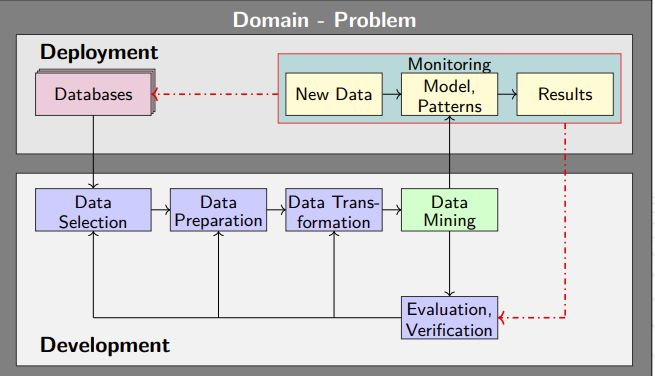
\includegraphics[width=\textwidth]{Images/KDD/KDDMonitoring}
	\caption{\textbf{Process Workflow}}
	
\end{figure}

\section{Introduction to \ac{kdd}}

Knowledge Discovery in Databases (\ac{kdd}) is a fundamental step in the broader knowledge discovery process. It refers to the systematic extraction of meaningful patterns, trends, and insights from large datasets. At its core, \ac{kdd} enables organizations and researchers to transform raw data into actionable knowledge. A key aspect of this process is data mining, which involves identifying interesting patterns within vast amounts of data.

By analyzing existing datasets, data mining facilitates the discovery of solutions to complex problems. This process involves leveraging historical data to build predictive models that anticipate future trends and behaviors. The ultimate objective of data mining is to uncover patterns that are not only valid and novel but also potentially useful and easily understandable. These insights often form the foundation for strategic decision-making across various industries.

\section{Types of Data Mining Tasks}

Data mining tasks can generally be classified into two primary categories: \textbf{descriptive tasks} and \textbf{predictive tasks}.

\subsection{Descriptive Tasks}
Descriptive data mining focuses on analyzing datasets to uncover inherent patterns and summarize their properties. These tasks help characterize the general attributes of data, providing insights into the underlying structure of the database. For example, clustering techniques can group similar data points, offering a better understanding of the dataset's composition.

\subsection{Predictive Tasks}
Predictive data mining, on the other hand, involves using historical data to forecast unknown or future trends. These tasks rely on identifying relationships between variables to make informed predictions. For instance, regression and classification models can predict customer behavior, sales trends, or market dynamics \cite{Fezari:2018}.

\section{Applications of Data Mining}

Data mining finds extensive applications across numerous industries, including:

\begin{itemize}
	\item \textbf{Healthcare:}  
	In medicine, data mining assists in analyzing patient records to predict disease progression, improve diagnostics, and tailor treatment plans. By identifying patterns in medical histories, healthcare providers can enhance patient care and operational efficiency.
	
	\item \textbf{Retail and Marketing:}  
	Retailers use data mining to understand consumer behavior, optimize pricing strategies, and personalize marketing campaigns. Analyzing sales data helps identify purchasing patterns, leading to better inventory management and targeted promotions.
	
	\item \textbf{Finance:}  
	In the financial sector, data mining plays a crucial role in fraud detection, credit scoring, and risk assessment. By analyzing transaction patterns, banks and financial institutions can mitigate risks and improve decision-making.
	
	\item \textbf{Telecommunications:}  
	Telecommunications companies use data mining to analyze customer usage patterns, predict churn rates, and improve service quality. These insights enable companies to develop more effective customer retention strategies.
	
	\item \textbf{Scientific Research:}  
	In science, data mining facilitates the analysis of large-scale datasets to uncover patterns and correlations that drive discoveries and innovations.
\end{itemize}

The insights derived from data mining empower organizations to improve profitability, enhance customer satisfaction, and optimize operations. The following sections delve deeper into specific data mining tasks and their methodologies.
	
\section{KDD for Magic Wand Project}
	
	The integration of Knowledge Discovery in Databases (\ac{kdd}) is a cornerstone in optimizing the design and performance of our Magic Wand project. This project leverages the Arduino Nano BLE 33, equipped with an accelerometer, to enable on-device gesture recognition. Through the application of \ac{kdd}, meaningful insights are derived from the extensive dataset generated by the device's accelerometer, enabling the seamless recognition and classification of predefined gestures.
	
	\subsection{Understanding Descriptive and Predictive Tasks}
	
	The application of \ac{kdd} in the Magic Wand project involves two primary categories of data mining tasks: descriptive and predictive.
	
	\begin{itemize}
		\item \textbf{Descriptive Tasks:}  
		Descriptive tasks focus on analyzing accelerometer data to uncover inherent functional patterns. These patterns help characterize the general properties of hand movements, offering valuable insights into the gestures' nature and variations. For instance, clustering similar motion patterns can highlight commonalities in user behavior, aiding in feature engineering for the recognition model.
		
		\item \textbf{Predictive Tasks:}  
		Predictive tasks utilize historical accelerometer data to anticipate future trends and behaviors. In the Magic Wand project, predictive modeling enables the system to identify and classify gestures in real time. By training the model on labeled datasets, it becomes capable of recognizing both simple and complex gestures with high accuracy.
	\end{itemize}
	
	\subsection{Applications of Data Mining in Gesture Recognition}
	
	Data mining, as a key component of \ac{kdd}, empowers the Magic Wand project to extract meaningful patterns from raw accelerometer data. This capability is instrumental in recognizing valid and novel hand gestures. The process involves feature extraction, pattern identification, and classification to ensure precise gesture recognition. By enhancing the accuracy and responsiveness of the system, data mining significantly improves user experience and system reliability \cite{Fezari:2018}.
	
	\subsection{Real-world Impact in Various Domains}
	
	The insights derived through \ac{kdd} extend the Magic Wand project's potential applications across multiple industries:
	
	\begin{itemize}
		\item \textbf{Healthcare:}  
		Gesture recognition systems powered by \ac{kdd} can assist in physical therapy, enabling patients to perform prescribed exercises while the system monitors and evaluates their movements.
		
		\item \textbf{Retail and Marketing:}  
		Retail environments can benefit from gesture-based interaction systems, such as virtual assistants or kiosks that respond to user gestures for navigation or selection.
		
		\item \textbf{Finance:}  
		In banking and finance, gesture recognition can facilitate secure authentication mechanisms and improve accessibility for individuals with disabilities.
		
		\item \textbf{Telecommunications:}  
		Gesture-based controls powered by data mining can enhance user interaction with smart devices, improving accessibility and functionality.
		
		\item \textbf{Science and Education:}  
		Gesture recognition systems can be used in educational tools to provide interactive learning experiences, especially in virtual or augmented reality environments \cite{Fezari:2018}.
	\end{itemize}
	\subsection{CRISP-DM}
The CRISP-DM process was developed by the means of the effort of a consortium initially composed with DaimlerChrysler, SPSS, and NCR. CRISP-DM stands for \textbf{Cross-Industry Standard Process for Data Mining}. It consists of a cycle that comprises six stages (Figure~2):  

\begin{enumerate}
    \item \textbf{Business understanding} – This initial phase focuses on understanding the project objectives and requirements from a business perspective, then converting this knowledge into a data mining problem definition and a preliminary plan designed to achieve the objectives.  

    \item \textbf{Data understanding} – The data understanding phase starts with an initial data collection and proceeds with activities in order to get familiar with the data, to identify data quality problems, to discover first insights into the data, or to detect interesting subsets to form hypotheses for hidden information.  

    \item \textbf{Data preparation} – The data preparation phase covers all activities to construct the final dataset from the initial raw data.  

    \item \textbf{Modeling} – In this phase, various modeling techniques are selected and applied, and their parameters are calibrated to optimal values.  

    \item \textbf{Evaluation} – At this stage, the model (or models) obtained is more thoroughly evaluated, and the steps executed to construct the model are reviewed to be certain it properly achieves the business objectives.  

    \item \textbf{Deployment} – Creation of the model is generally not the end of the project. Even if the purpose of the model is to increase knowledge of the data, the knowledge gained will need to be organized and presented in a way that the customer can use it.  
\end{enumerate}

 

\begin{figure}[h]
    \centering
    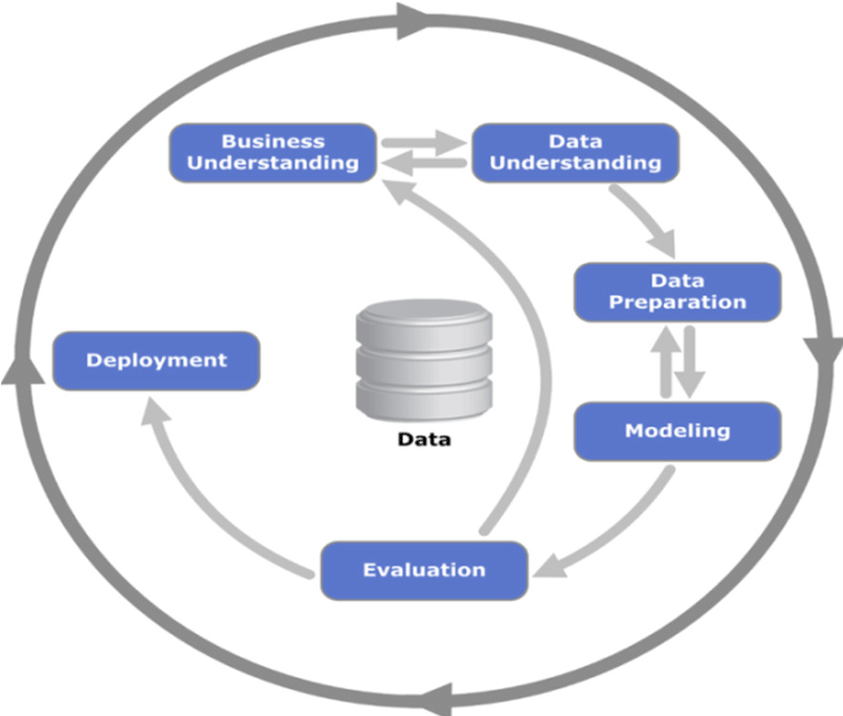
\includegraphics[width=0.8\textwidth]{Images/Methodology/figure2.png}
    \caption{The CRISP-DM life cycle (Chapman et al., 2000)}
\end{figure}

The sequence of the six stages is not rigid, as is schematized in Figure~2. CRISP-DM is extremely complete and documented. All its stages are duly organized, structured, and defined, allowing that a project could be easily understood or revised (Santos \& Azevedo, 2005). Although the CRISP-DM process is independent from the DM chosen tool, it is linked to the SPSS Clementine software.  


\subsection{Comparison of KDD and CRISP-DM}
\begin{table}[h!]
    \centering
    \begin{tabular}{@{}p{3.5cm}p{5.5cm}p{5.5cm}@{}}
        \toprule
        \textbf{Aspect} & \textbf{KDD (Knowledge Discovery in Databases)} & \textbf{CRISP-DM (Cross-Industry Standard Process for Data Mining)} \\ \midrule
        \textbf{Origin and Scope} & Focused on the overall process of extracting knowledge from databases. & Aimed at structuring data mining projects in a business or industrial setting. \\ \midrule
        \textbf{Phases} & 
        \begin{enumerate}
            \item Data Selection
            \item Data Preprocessing
            \item Data Transformation
            \item Data Mining
            \item Interpretation/Evaluation
        \end{enumerate} &
        \begin{enumerate}
            \item Business Understanding
            \item Data Understanding
            \item Data Preparation
            \item Modeling
            \item Evaluation
            \item Deployment
        \end{enumerate} \\ \midrule
        \textbf{Flexibility} & High flexibility, emphasizes iterative exploration and hypothesis testing. & Prescriptive and structured, with an emphasis on well-documented steps for business clarity. \\ \midrule
        \textbf{Tool Independence} & Independent of tools and platforms. & Initially linked to SPSS Clementine (now IBM SPSS Modeler). \\ \midrule
        \textbf{Target Audience} & Academics and technical experts focused on novel insights and experimental exploration. & Business professionals requiring a structured, repeatable process for solving problems. \\ \midrule
        \textbf{Documentation Emphasis} & Less formalized; focuses on the iterative discovery of knowledge. & High emphasis on documentation for ease of project understanding and reproducibility. \\ 
        \bottomrule
    \end{tabular}
    \caption{Comparison of KDD and CRISP-DM}
    \label{tab:comparison}
\end{table}

\subsection{Why KDD is Better for the Magic Wand Project}
The magic wand project using the Arduino Nano 33 BLE Sense involves real-time sensor data processing and gesture recognition. Below are key reasons why KDD is better suited:

\begin{enumerate}
    \item \textbf{Focus on Sensor Data Processing} 
    The Arduino Nano 33 BLE Sense provides raw sensor data (e.g., accelerometer, gyroscope, magnetometer). KDD emphasizes \textit{data preprocessing} and \textit{transformation}, which are essential for converting raw data into meaningful features (e.g., gesture patterns). KDD's iterative nature allows for fine-tuning these transformations, crucial for a real-time system like the magic wand.

    \item \textbf{Exploratory Nature of KDD} 
    The magic wand project involves \textit{exploring gestures} and creating patterns using embedded sensors. KDD allows repeated hypothesis testing and refinement, enabling the discovery of novel gesture mappings or better feature extraction techniques.

    \item \textbf{Less Emphasis on Business Objectives} 
    CRISP-DM’s \textit{business understanding phase} is less relevant for this project, which is \textit{experimental and technical} rather than business-driven. KDD focuses directly on the data and knowledge discovery, aligning well with the goals of the magic wand.

    \item \textbf{Tool Independence} 
    KDD is tool-agnostic and compatible with \textit{open-source platforms} like Arduino. CRISP-DM, initially linked to SPSS Clementine (a proprietary tool), is less adaptable for hardware-based projects.

    \item \textbf{Iterative Feedback} 
    In KDD, the iterative cycle between preprocessing, transformation, and data mining is critical for adapting to sensor noise or calibration changes. This feedback loop is vital for optimizing gesture recognition in the magic wand project.
\end{enumerate}

KDD is better suited for the \textit{magic wand project using Arduino Nano 33 BLE Sense} because it provides the flexibility needed to work with raw sensor data, emphasizes preprocessing and transformation, and facilitates iterative exploration and optimization of gesture recognition models. These aspects align closely with the challenges and goals of the project, making KDD the ideal methodology.


\subsection{ML Pipeline}

\subsection{1. Data Selection}
\textbf{Objective}: Identify and collect relevant sensor data.  
\begin{itemize}
    \item Use the embedded sensors (e.g., accelerometer, gyroscope, magnetometer) on the Arduino Nano 33 BLE Sense.
    \item Define the gestures to be recognized (e.g., wave, circle, swipe).
    \item Collect sensor data for each gesture, ensuring variation in speed, orientation, and user input.
    \item Store raw data for each axis (X, Y, Z) over time.
\end{itemize}
\textbf{Tools}: Arduino IDE for data logging, serial communication, or an SD card for storage.

\subsection{2. Data Preprocessing}
\textbf{Objective}: Clean and prepare raw sensor data for analysis.  
\begin{itemize}
    \item \textbf{Data Cleaning}: Remove noise and outliers using filters (e.g., low-pass filter to remove high-frequency noise).
    \item \textbf{Data Resampling}: Normalize sampling rates for consistent data across all gestures.
    \item \textbf{Windowing}: Segment data into fixed-size time windows (e.g., 1-second windows) to capture meaningful patterns.
    \item \textbf{Scaling}: Normalize sensor values to a consistent range (e.g., [-1, 1] or [0, 1]).
\end{itemize}
\textbf{Tools}: Python (e.g., NumPy, Pandas), Arduino libraries (e.g., filters).

\subsection{3. Data Transformation}
\textbf{Objective}: Extract features from the preprocessed data.  
\begin{itemize}
    \item Compute statistical features like mean, variance, standard deviation, energy, and entropy for each window.
    \item Calculate domain-specific features (e.g., Fast Fourier Transform (FFT) for frequency analysis).
    \item Combine features from multiple sensors (e.g., accelerometer + gyroscope).
    \item Encode gestures into labeled data (e.g., ``gesture\_1'', ``gesture\_2'').
\end{itemize}
\textbf{Tools}: Python (e.g., SciPy, sklearn), MATLAB (if needed).

\subsection{4. Data Mining (Modeling)}
\textbf{Objective}: Train a machine learning model to classify gestures.  
\begin{itemize}
    \item \textbf{Split the dataset}: Use an 80-20 train-test split.
    \item \textbf{Model Selection}: Choose lightweight models suitable for edge devices, such as:
          \begin{itemize}
              \item Decision Trees
              \item Random Forest
              \item k-Nearest Neighbors (k-NN)
              \item Neural Networks (e.g., TensorFlow Lite for microcontrollers)
          \end{itemize}
    \item \textbf{Training}: Optimize hyperparameters (e.g., tree depth, number of neighbors).
    \item \textbf{Validation}: Use cross-validation to ensure model generalization.
\end{itemize}
\textbf{Tools}: TensorFlow Lite, Edge Impulse, or sklearn.

\subsection{5. Interpretation/Evaluation}
\textbf{Objective}: Evaluate model performance and refine it.  
\begin{itemize}
    \item \textbf{Metrics}:
          \begin{itemize}
              \item Accuracy, precision, recall, and F1-score.
              \item Confusion matrix to analyze gesture misclassifications.
              \item Latency and memory usage to ensure real-time performance on the Arduino.
          \end{itemize}
    \item \textbf{Steps}:
          \begin{itemize}
              \item Test the model on unseen gesture data.
              \item Evaluate performance under real-world conditions (e.g., different lighting or motion speeds).
          \end{itemize}
\end{itemize}
\textbf{Tools}: Arduino Nano's onboard resources for testing, Python for analysis.

\subsection{6. Deployment}
\textbf{Objective}: Deploy the trained model onto the Arduino Nano 33 BLE Sense.  
\begin{itemize}
    \item Convert the model into a format suitable for the Arduino (e.g., TensorFlow Lite format).
    \item Integrate the model with gesture recognition logic using Arduino libraries.
    \item Test gesture recognition in real-time and refine thresholds or logic as needed.
    \item Optimize for power consumption and memory.
\end{itemize}
\textbf{Tools}: TensorFlow Lite for Microcontrollers, Arduino IDE, Edge Impulse Studio.

\subsection{Pipeline Flow Diagram}
\[
\text{Sensor Data Collection} \rightarrow \text{Preprocessing} \rightarrow \text{Feature Extraction} \rightarrow \text{Model Training} \rightarrow \text{Evaluation} \rightarrow \text{Deployment}
\]

	
	\subsection{Conclusion}
	
	By employing the principles of \ac{kdd}, the Magic Wand project effectively harnesses the potential of data mining to analyze and understand hand movements. This approach ensures accurate and real-time gesture recognition, paving the way for innovative applications across diverse industries.
	


%%%%%%%%%%%%
%
% $Autor: Adhiraj $
% $Datum: 2024-12-25 08:03:15Z $
% $Pfad: TemplateSensor $
% $Version: 4250 $
% !TeX spellcheck = en_GB/de_DE
% !TeX encoding = utf8
% !TeX root = Algorithm 
% !TeX TXS-program:bibliography = txs:///biber
%
%%%%%%%%%%%%


\chapter{Convolutional Neural Networks(CNN)}

\section{Introduction}

Recent advancements in artificial intelligence, particularly in deep learning, have significantly impacted various cutting-edge technology applications, ranging from autonomous vehicles to creative fields like music and art generation. A central ambition within the scientific community is to enable computers to communicate and comprehend language in a manner akin to human interaction \cite{Li:2021}. As a subset of machine learning, deep learning stands out due to its focus on learning data representations rather than relying on predefined task-specific algorithms. This methodology empowers systems to build complex concepts by integrating information from simpler, fundamental elements.

A Convolutional Neural Network (CNN) has been selected to develop the model, building upon and enhancing the ideas proposed by Warden and Giménez \cite{Warden:2020}. This choice makes CNN an ideal candidate for applications in voice recognition.

Convolutional Neural Networks (CNNs) are a specialized type of multi-layer neural network designed to identify visual patterns in images directly with minimal preprocessing. In artificial neural networks, a neuron serves as a transformative unit that processes inputs to produce outputs. The number of neurons utilized varies based on the specific task and can range from a few to several thousand. Artificial neurons are interconnected in various configurations to form a CNN. Within this structure, individual neurons receive inputs from others, with each input's weight determining its positive or negative influence. 

The collective learning of the network enables it to perform critical computations required for tasks like object recognition and language understanding. These interconnected neurons form a feed-forward network, where outputs from one layer are passed to subsequent layers. This process continues until a final output is generated \cite{Gu:2018}.


\section{Description}

Understanding the internal mechanisms of the model is not essential for its application; however, exploring these processes can be valuable for addressing potential issues and is intrinsically engaging. This section provides an overview of the model's predictive functionality. Within neural network architecture, a specific type excels in managing multidimensional tensors by leveraging the relationships between neighboring values—known as a Convolutional Neural Network (CNN). Although typically used for image processing, where inputs are 2D pixel grids, CNNs demonstrate exceptional adaptability in analyzing spectrogram data, highlighting their utility beyond traditional visual tasks \cite{Warden:2020}.
This section introduces the basic concepts of CNN. Furthermore, descriptions of crucial elements including the optimizer, loss function, and activation function.

\subsection{CNN Components}

Convolutional Neural Networks (CNNs) are a type of feedforward neural network that excel in automatically extracting features from data through their convolutional architecture. Unlike traditional methods that rely on manual feature extraction, CNNs streamline this process by learning features directly from the data. Inspired by visual perception, CNNs employ kernels that act as artificial receptors, detecting various features and aligning artificial neurons with the behavior of biological neurons. 

Activation functions, analogous to the biological threshold for signal transmission, simulate the electrical signaling between neurons. Meanwhile, loss functions and optimizers play a critical role in guiding the CNN to identify and learn the desired patterns effectively \cite{Li:2021}.

Compared to fully connected (FC) networks (see Figure \ref{fig:CNNandFCLayers}), CNNs offer several advantages:

\begin{itemize}
	\item \textbf{Localized Connections:} In CNNs, neurons connect only to a subset of the previous layer rather than all neurons, reducing parameters and computational complexity. This structure helps focus on spatially relevant features and speeds up convergence.
	\item \textbf{Weight Sharing:} A single set of weights is reused across different locations in the input, capturing patterns like edges regardless of position. This reduces parameters and improves generalization.
	\item \textbf{Downsampling:} Pooling layers summarize data by retaining key features (e.g., max or average values), reducing spatial dimensions and computational cost while eliminating redundant information.
\end{itemize}


\begin{figure}[h!]
	\centering
	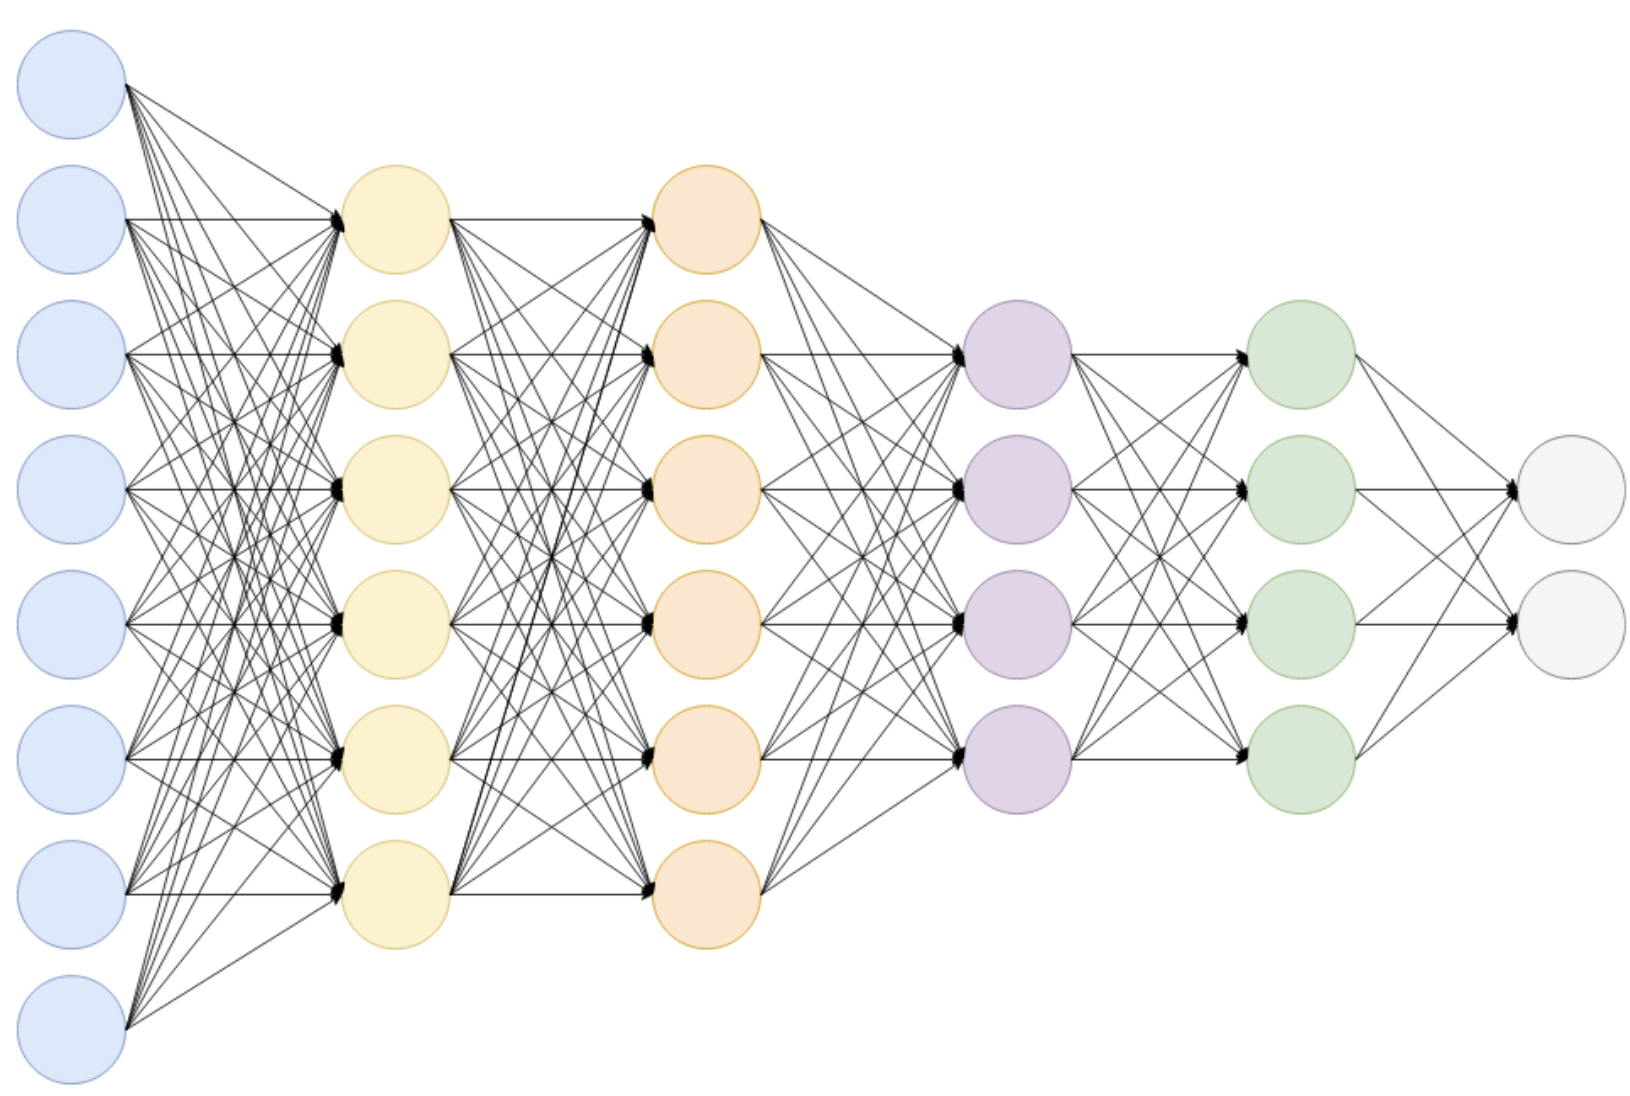
\includegraphics[width=0.8\textwidth]{Images/Algorithm/CNNandFCLayers}
	\caption{CNN and FC layers \cite{Wings:2023}} \label{fig:CNNandFCLayers}
\end{figure}


Convolution is a key step in the feature extraction process, generating feature maps. Padding, achieved by adding zero values to the input, helps prevent information loss at the edges of the input. Stride controls the density of the convolution operation. However, the feature maps produced can lead to overfitting, necessitating the use of pooling (either max pooling or average pooling) to eliminate redundant information. Figure \ref{fig:ProcedureCNN} illustrates the overall CNN workflow. Below is a detailed explanation of padding, stride, and pooling \cite{Li:2021}:

\begin{itemize}
	\item \textbf{Padding:} Padding refers to the addition of extra pixels around the edges of the input image before the convolution process. This is typically done by surrounding the image with rows and columns filled with zeros. The purpose of padding is to prevent the loss of information at the image borders during convolution.
	
	\item \textbf{Stride:} Stride refers to the step size, or the number of pixels the convolution filter moves across the image during the convolution operation. A larger stride results in smaller feature maps, which leads to a more compact representation.
	
	\item \textbf{Pooling:} Pooling is a down-sampling technique applied after convolution that reduces the size of the feature maps. It helps control the number of parameters in the network. Common pooling methods include max pooling and average pooling \cite{Wings:2023}.
	
	\begin{enumerate}
		\item \textbf{Max Pooling:} Max pooling is a pooling operation where, for each region of the feature map, the highest value is selected. This preserves the most important features from that region, providing a compact summary of the spatial information.
		
		\item \textbf{Average Pooling:} Average pooling is another pooling method where the average value of each region in the feature map is computed. This technique reduces the spatial dimensions while preserving a smoother, less detailed version of the features.
	\end{enumerate}
\end{itemize}

\begin{figure}[h!]
	\centering
	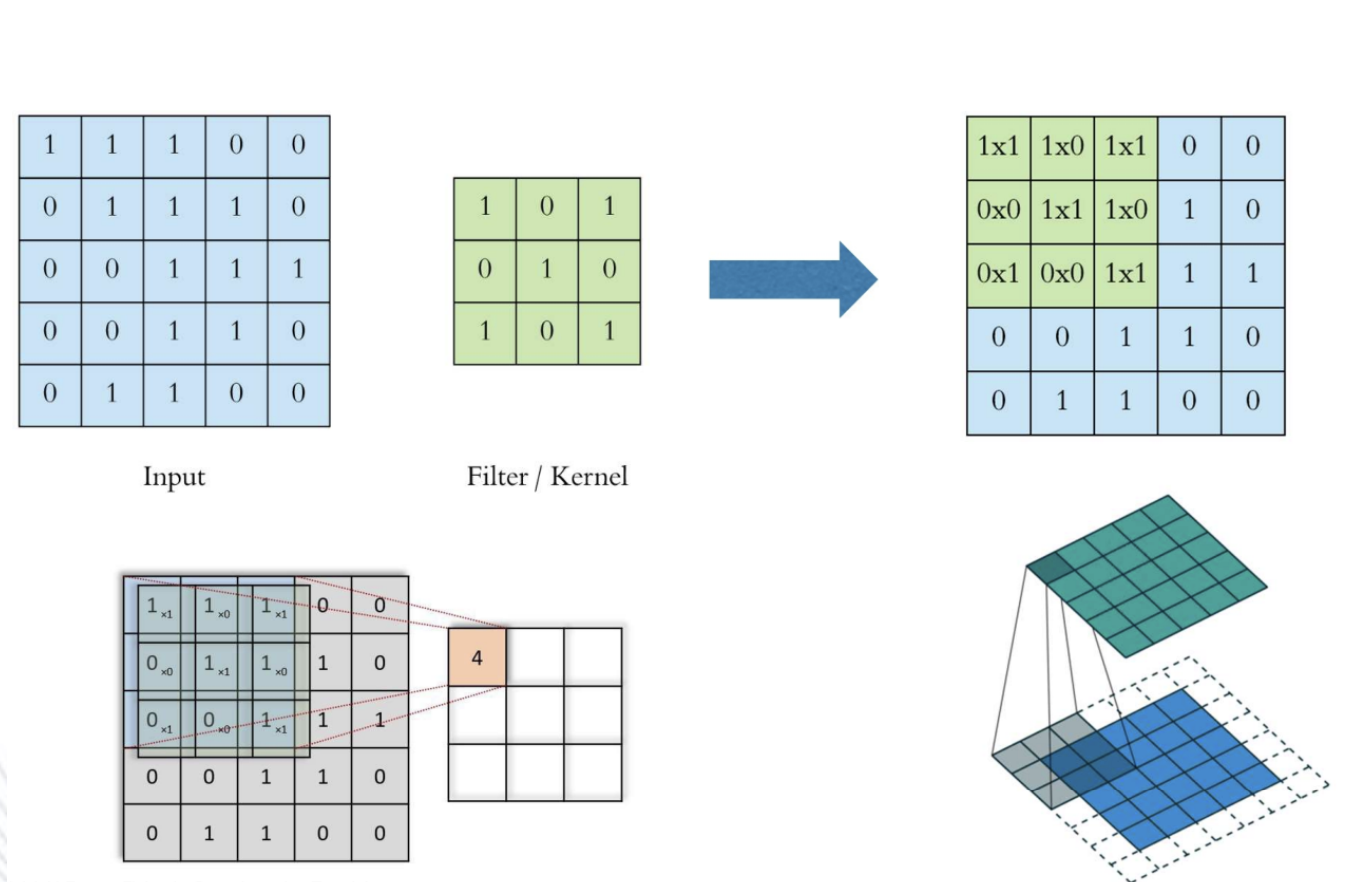
\includegraphics[width=0.8\textwidth]{Images/Algorithm/ProcedureCNN}
	\caption{Procedure of a two-dimensional CNN} \label{fig:ProcedureCNN}
\end{figure}

The field of Convolutional Neural Networks (CNNs) includes numerous architectural variations, but their fundamental components remain consistent. For instance, the well-known LeNet-5 architecture consists of three primary layers: convolutional, pooling, and fully-connected layers \cite{Gu:2018}. The primary role of the convolutional layer is to extract meaningful feature representations from the input data.

As illustrated in Figure \ref{subfig:LetNet5ArchitectureNetwork}, the convolutional layer comprises multiple convolutional kernels, each responsible for generating unique feature maps. Each neuron in a feature map is connected to a specific region of neurons in the preceding layer, referred to as its receptive field. The creation of a feature map involves convolving the input data with a learned kernel, followed by applying an element-wise nonlinear activation function. Importantly, each feature map is generated by sharing the kernel across all spatial regions of the input, with multiple distinct kernels utilized to produce the complete set of feature maps.

\begin{figure}[h!]
	\centering
	
	\begin{subfigure}{0.65\textwidth}
		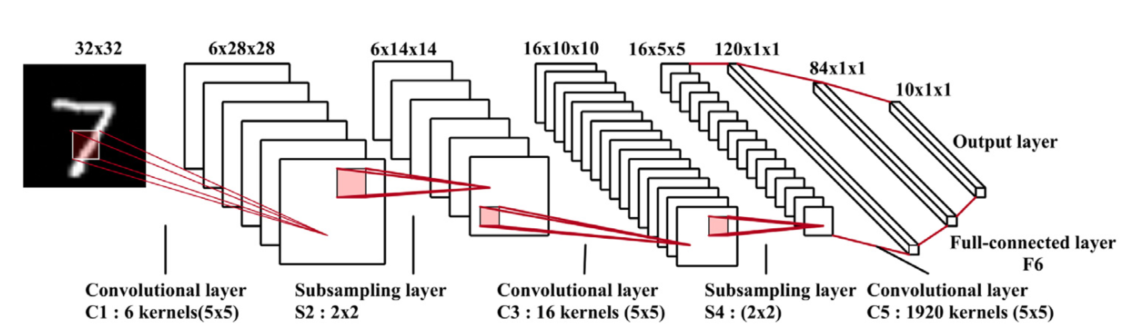
\includegraphics[width=\linewidth]{Images/Algorithm/LetNet5ArchitectureNetwork}
		\caption{LetNet-5 network}    % \caption{} is kept to keep (a), (b), (c) etc. below each subfigure.
		\label{subfig:LetNet5ArchitectureNetwork}
	\end{subfigure}
	\hfill
	\begin{subfigure}{0.3\textwidth}
		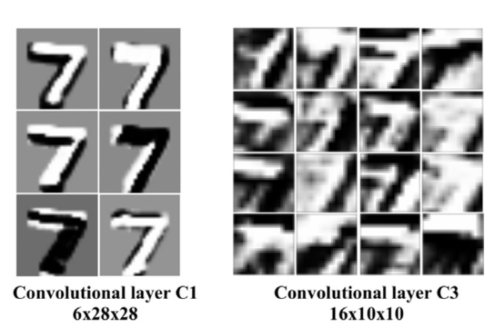
\includegraphics[width=\linewidth]{Images/Algorithm/LetNet5ArchitectureLearnedFeatures}
		\caption{Learned features}    % \caption{} is kept to keep (a), (b), (c) etc. below each subfigure.
		\label{subfig:LetNet5ArchitectureLearnedFeatures}
	\end{subfigure}
	
	\caption{The architecture of the LeNet-5 network \cite{Gu:2018}. (\subref{subfig:LetNet5ArchitectureNetwork}) The architecture of the LeNet-5 network, renowned for its effectiveness in digit classification tasks. (\subref{subfig:LetNet5ArchitectureLearnedFeatures}) Displaying the features within the LeNet-5 network through visualizations, where each layer's feature maps are showcased in distinct blocks.}
	\label{fig:LetNet5Architecture}
\end{figure}

Mathematically, the feature value at location $(i, j)$ in the $k$th feature map of the $l$th layer (denoted as $z^l_{i,j,k}$) is computed by the expression:

\begin{equation}
	z^l_{i,j,k} = {\mathbf{w}^l_k}^T \mathbf{x}^l_{i,j} + b^l_k
\end{equation}

Here, $\mathbf{w}^l_k$ and $b^l_k$ denote the weight vector and bias term of the $k$th filter in the $l$th layer, respectively, while $\mathbf{x}^l_{i,j}$ represents the input patch centered at location $(i, j)$ in the $l$th layer. The weight-sharing mechanism, where the same kernel is used to generate the feature map across the input, helps reduce model complexity and improves the efficiency of network training.

The activation function ($a(\cdot)$) introduces nonlinearity into the CNN, which is essential for detecting complex, nonlinear patterns in multi-layer networks. The activation value ($a_{l,i,j,k}$) of the convolutional feature $z_{l,i,j,k}$ is calculated as:

\begin{equation}
	a^l_{i,j,k} = a(z^l_{i,j,k})
\end{equation}

Common activation functions include sigmoid, tanh, and ReLU.The pooling layer, positioned between convolutional layers, aims to achieve shift-invariance by downsampling the feature maps' resolution. Each feature map in the pooling layer connects to its corresponding feature map in the preceding convolutional layer. The pooling operation, denoted as $\mathrm{pool}(\cdot)$, is applied to each feature map $a^l_{m,n,k}$ with:

\begin{equation}
	y^l_{i,j,k} = \mathrm{pool}(a^l_{m,n,k}), \forall (m, n) \in \mathcal{R}_{ij}
\end{equation}

In this context, $\mathcal{R}_{ij}$ represents a local neighborhood around the location $(i, j)$. Common pooling techniques include average pooling and max pooling. As shown in Figure \ref{subfig:LetNet5ArchitectureLearnedFeatures} for the digit 7, the learned feature maps progressively capture hierarchical patterns. Early layers extract low-level features, such as edges and curves, while deeper layers encode more abstract and high-level representations.

After the convolutional and pooling layers, one or more fully-connected layers are often used for high-level reasoning. These layers establish dense connections by linking all neurons from the previous layer to each neuron in the current layer, generating global semantic representations. A fully-connected layer can also be replaced by a $1 \times 1$ convolutional layer to achieve similar functionality.

The final layer in CNNs serves as the output layer. For classification tasks, the softmax function is frequently used. Alternatively, CNN features can be combined with Support Vector Machines (SVM) to address various classification challenges. Let the desired input-output relationships be represented as $\{(\mathbf{x}^{(n)}, \mathbf{y}^{(n)}); n \in [1, \ldots, N]\}$. The CNN parameters, denoted by $\mathbf{\theta}$ (including weight vectors and bias terms), are optimized by minimizing a task-specific loss function:


\begin{equation}
	\mathcal{L} = \frac{1}{N} \sum_{n=1}^{N} \ell(\mathbf{\theta}; \mathbf{y}^{(n)}, \mathbf{o}^{(n)})
\end{equation}

Here, $\mathcal{L}$ represents the loss function, which quantifies the discrepancy between the predicted output ($\mathbf{o}^{(n)}$) and the actual target label ($\mathbf{y}^{(n)}$) for $n$th input data point $\mathbf{x}^{(n)}$. The symbol $\mathbf{\theta}$ denotes all the parameters of the CNN, including weight vectors and bias terms. The function $\ell(\mathbf{\theta}; \mathbf{y}^{(n)}, \mathbf{o}^{(n)})$ is the individual loss for a specific data point, measuring the dissimilarity between the predicted output and the true label. The goal during training is to minimize the average loss over all data points, achieved through techniques such as stochastic gradient descent.

The training of a CNN involves global optimization, with the aim of finding the best set of parameters by minimizing the loss function. Stochastic gradient descent emerges as a common solution for optimizing CNN networks, providing an effective means of iterative parameter adjustment.  

\subsection{Activation Function}
\label{subsection:ActivationFunction}

Convolutional Neural Networks (CNNs) utilize a variety of activation functions to capture complex features \cite{Li:2021}. Similar to the behavior of neurons in the human brain, the activation function acts as a mechanism that determines whether information is passed to the next neuron. In a multilayer neural network, activation functions are positioned between layers, as shown in Figure \ref{fig:activationFunctionStructure}.

In Figure \ref{fig:activationFunctionStructure}, $x_i$ represents the input features, with $n$ features simultaneously fed into neuron $j$. The term $w_{ij}$ corresponds to the weight of the connection between input feature $x_i$ and neuron $j$, $b_j$ represents the bias (internal state) of neuron $j$, and $y_j$ is the neuron's output. The activation function, denoted as $f(\cdot)$, may include options such as sigmoid, tanh, or rectified linear unit (ReLU), among others.

If no activation function or a linear activation function is applied, the network’s output becomes a simple linear combination of the inputs, which restricts its learning ability. Introducing nonlinear activation functions, such as sigmoid or tanh, enables the network to model and fit more complex patterns in the data.

\begin{figure}[h!]
	\centering
	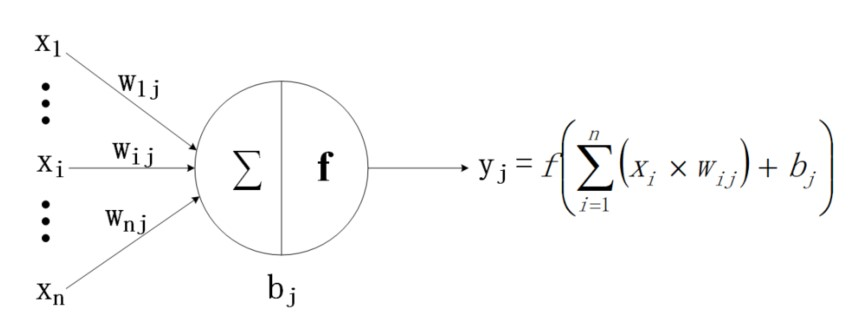
\includegraphics[width=0.6\textwidth]{Images/Algorithm/activationFunctionStructure}
	\caption{Structure of an activation function \cite{Li:2021}.} \label{fig:activationFunctionStructure}
\end{figure}

Some of the well-known actiovatoion functions are shown in the Figure \ref{fig:activationFunctions}. The sigmoid function maps a real number to (0, 1), suitable for binary classification. The tanh function maps to (-1, 1), aiding normalization. ReLU, with its advantages in learning speed, is preferred in deep networks. Leaky ReLU and PReLU address limitations of ReLU, reducing neuron inactivation. ELU improves convergence by having a negative output average.

Swish, proposed by Google, and mish, a novel activation function, demonstrate improved performance compared to ReLU and Swish in deeper models across diverse datasets. mish, in particular, exhibits superior gradient flow, accuracy, and generalization properties. Experimental results consistently support the effectiveness of Mish across standard architectures.

\begin{figure}[h!]
	\centering
	
	\begin{subfigure}{0.22\textwidth}
		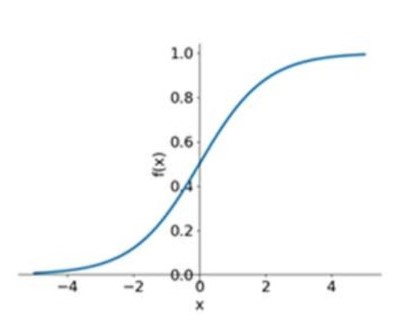
\includegraphics[width=\linewidth]{Images/Algorithm/SigmoidFunction}
		\caption{}    % \caption{} is kept to keep (a), (b), (c) etc. below each subfigure.
		\label{subfig:Sigmoid}
	\end{subfigure}
	\hfill
	\begin{subfigure}{0.22\textwidth}
		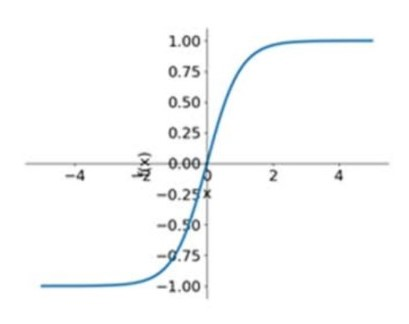
\includegraphics[width=\linewidth]{Images/Algorithm/TanhFunction}
		\caption{}    % \caption{} is kept to keep (a), (b), (c) etc. below each subfigure.
		\label{subfig:Tanh}
	\end{subfigure}
	\hfill
	\begin{subfigure}{0.22\textwidth}
		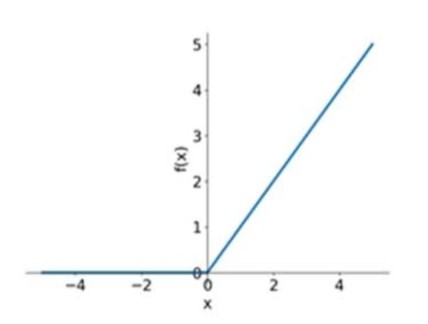
\includegraphics[width=\linewidth]{Images/Algorithm/ReLUFunction}
		\caption{}    % \caption{} is kept to keep (a), (b), (c) etc. below each subfigure.
		\label{subfig:ReLU}
	\end{subfigure}
	\hfill
	\begin{subfigure}{0.22\textwidth}
		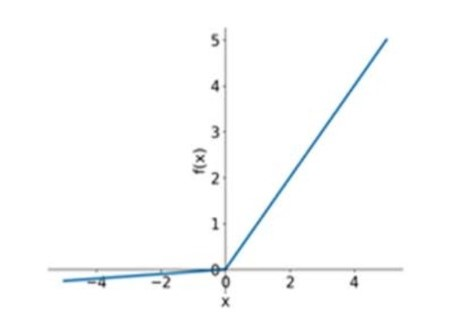
\includegraphics[width=\linewidth]{Images/Algorithm/LeakyReLUFunction}
		\caption{}    % \caption{} is kept to keep (a), (b), (c) etc. below each subfigure.
		\label{subfig:LeakyReLU}
	\end{subfigure}
	
	\medskip
	
	\begin{subfigure}{0.22\textwidth}
		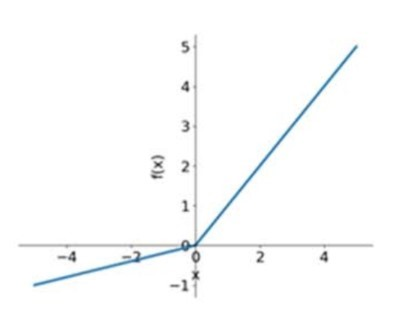
\includegraphics[width=\linewidth]{Images/Algorithm/PReLUFunction}
		\caption{}    % \caption{} is kept to keep (a), (b), (c) etc. below each subfigure.
		\label{subfig:PReLU}
	\end{subfigure}
	\hfill
	\begin{subfigure}{0.22\textwidth}
		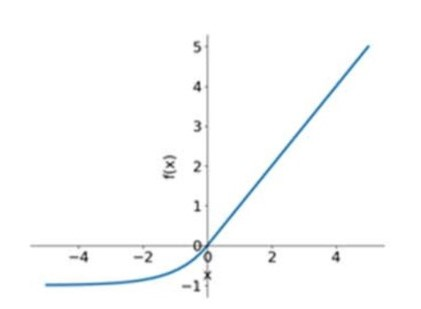
\includegraphics[width=\linewidth]{Images/Algorithm/ELUFunction}
		\caption{}    % \caption{} is kept to keep (a), (b), (c) etc. below each subfigure.
		\label{subfig:ELU}
	\end{subfigure}
	\hfill
	\begin{subfigure}{0.22\textwidth}
		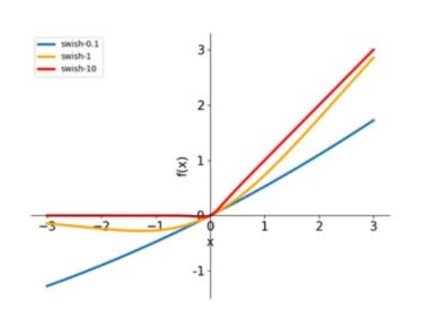
\includegraphics[width=\linewidth]{Images/Algorithm/SwishFunctions}
		\caption{}    % \caption{} is kept to keep (a), (b), (c) etc. below each subfigure.
		\label{subfig:Swish}
	\end{subfigure}
	\hfill
	\begin{subfigure}{0.22\textwidth}
		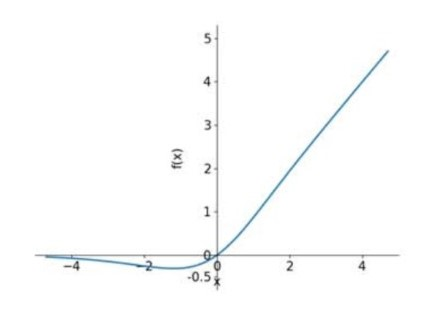
\includegraphics[width=\linewidth]{Images/Algorithm/MishFunction}
		\caption{}    % \caption{} is kept to keep (a), (b), (c) etc. below each subfigure.
		\label{subfig:Mish}
	\end{subfigure}
	
	\caption{Diagrams of activation functions \cite{Li:2021}.  (\subref{subfig:Sigmoid}) Sigmoid function.  (\subref{subfig:Tanh}) Tanh function. (\subref{subfig:ReLU}) ReLU function. (\subref{subfig:LeakyReLU}) Leaky ReLU function. (\subref{subfig:PReLU}) PReLU function. (\subref{subfig:ELU}) ELU function.  (\subref{subfig:Swish}) Swish function. (\subref{subfig:Mish}) Mish function.}
	\label{fig:activationFunctions}
\end{figure}

\subsubsection{Guidelines for Activation Function Selection}

Choosing the right activation function is critical for optimizing the performance of a neural network. Below are some general guidelines to assist in selecting an appropriate activation function:

\begin{enumerate}
	\item For \textbf{binary classification} tasks, use the sigmoid function in the output layer, as it effectively maps outputs to probabilities between 0 and 1. For \textbf{multiclass classification}, the softmax function is more suitable as it normalizes outputs into a probability distribution across multiple classes.
	
	\item While the sigmoid and tanh functions are effective for introducing nonlinearity, they may cause \textbf{gradient vanishing problems}, especially in deep networks. To mitigate this, activation functions like ReLU (Rectified Linear Unit) or leaky ReLU are recommended for hidden layers, as they provide faster convergence and avoid saturation.
	
	\item When there is \textbf{uncertainty} about which activation function to use, ReLU or leaky ReLU can serve as reliable starting points, offering simplicity and consistent performance in most scenarios.
	
	\item If a large number of neurons become \textbf{inactive} during training, resulting in the "dying ReLU" problem, consider alternatives such as leaky ReLU, Parametric ReLU (PReLU), or exponential linear unit (ELU). These activation functions ensure that inactive neurons can still contribute to the learning process.
	
	\item To \textbf{speed up training}, set the negative slope of leaky ReLU to a small value like 0.02. This adjustment prevents neurons from becoming entirely inactive and facilitates faster convergence, particularly in challenging optimization landscapes.
\end{enumerate}

\subsubsection{Guidelines for Activation Function Selection}

Choosing the right activation function is critical for optimizing the performance of a neural network. Below are some general guidelines to assist in selecting an appropriate activation function:

\begin{enumerate}
	\item For \textbf{binary classification} tasks, use the sigmoid function in the output layer, as it effectively maps outputs to probabilities between 0 and 1. For \textbf{multiclass classification}, the softmax function is more suitable as it normalizes outputs into a probability distribution across multiple classes.
	
	\item While the sigmoid and tanh functions are effective for introducing nonlinearity, they may cause \textbf{gradient vanishing problems}, especially in deep networks. To mitigate this, activation functions like ReLU (Rectified Linear Unit) or leaky ReLU are recommended for hidden layers, as they provide faster convergence and avoid saturation.
	
	\item When there is \textbf{uncertainty} about which activation function to use, ReLU or leaky ReLU can serve as reliable starting points, offering simplicity and consistent performance in most scenarios.
	
	\item If a large number of neurons become \textbf{inactive} during training, resulting in the "dying ReLU" problem, consider alternatives such as leaky ReLU, Parametric ReLU (PReLU), or exponential linear unit (ELU). These activation functions ensure that inactive neurons can still contribute to the learning process.
	
	\item To \textbf{speed up training}, set the negative slope of leaky ReLU to a small value like 0.02. This adjustment prevents neurons from becoming entirely inactive and facilitates faster convergence, particularly in challenging optimization landscapes.
\end{enumerate}
Here’s the expanded version with added details and the corresponding LaTeX code:

\subsection{Optimizer}
\label{subsection:optimizer}

In CNNs, optimizing nonconvex functions is a critical step, often requiring robust optimizers to efficiently minimize the loss function within a reasonable timeframe \cite{Li:2021}. Nonconvex functions present complex landscapes with multiple local optima, making optimization challenging. These functions lack the convex property, where a line segment connecting any two points lies entirely within the function's domain, complicating the search for a global minimum. Effective optimization is crucial for improving model accuracy and convergence speed.

\subsubsection{Gradient Descent}

Gradient descent is a fundamental technique for training CNNs, with three common variants: batch gradient descent (BGD), stochastic gradient descent (SGD), and mini-batch gradient descent (MBGD).

\begin{itemize}
	\item \textbf{Batch Gradient Descent (BGD):} BGD calculates the average gradient over the entire dataset for each update. While it provides a stable descent direction, it is computationally expensive and impractical for large datasets due to memory constraints.
	\item \textbf{Stochastic Gradient Descent (SGD):} SGD updates the model parameters using a single data sample per iteration, making it suitable for online learning. However, it can result in high variance and oscillatory convergence due to noisy updates.
	\item \textbf{Mini-Batch Gradient Descent (MBGD):} MBGD strikes a balance between BGD and SGD by computing updates using small batches of data. It reduces variance compared to SGD and is computationally efficient, making it a popular choice for modern deep learning tasks.
\end{itemize}

\begin{itemize}
	\item \textbf{Gradient Descent Optimization Algorithms}
	
	Several advanced algorithms based on MBGD have been developed to address its limitations:
	
	\begin{itemize}
		\item \textbf{Momentum:} Introduces a velocity term to accelerate convergence and reduce oscillations in the optimization path.
		\item \textbf{Nesterov Accelerated Gradient (NAG):} Improves momentum by predicting the next position, allowing the optimizer to slow down when approaching steep slopes.
		\item \textbf{Adagrad:} Adapts the learning rate for each parameter, making it effective for sparse datasets, though it suffers from a monotonically decreasing learning rate.
		\item \textbf{Adadelta:} Addresses the diminishing learning rate issue in Adagrad by limiting updates to a window of recent gradients.
		\item \textbf{RMSprop:} Modifies Adagrad by normalizing gradients using an exponentially decaying average, maintaining a consistent learning rate.
		\item \textbf{Adam:} Combines the benefits of momentum and RMSprop, making it versatile and widely used in CNNs.
		\item \textbf{Other Variants:} Algorithms like AdaMax, Nadam, and AMSGrad provide further enhancements to address specific issues like stability and overshooting.
	\end{itemize}
	
	\item \textbf{Guidelines for Optimizer Selection:}
	\begin{enumerate}
		\item Employ \textbf{Mini-Batch Gradient Descent (MBGD)} for a balance between computational efficiency and gradient stability.
		\item Recognize that optimizer performance depends on the dataset's characteristics. According to the \textbf{No Free Lunch Theorem}, no optimizer is universally superior, so selection should be based on the task requirements and data distribution.
		\item If convergence issues such as oscillation or divergence occur, consider reducing the learning rate to stabilize updates.
	\end{enumerate}
\end{itemize}

\subsection{Feature Extraction}

In feature extraction, convolutional layers (convolutional layer and pooling layer) are extracted from a trained CNN and a new classifier, i.e. a fully connected layer with new classifications, is added. Two problems arise in this process:

\begin{itemize}
	\item The representation only contains information about the probability of occurrence of the class trained in the basic model.
	\item The fully connected layer contains no information about where the object is located.
\end{itemize}

Should the position of an object in the image matter, the fully connected layers are largely useless, as the later layers only generate abstract concepts. \cite{Chollet:2018}

\subsection{AlexNet}
The most popular CNNs for object detection and classification from image data are AlexNet, GoogleNet and ResNet50. \cite{Sharma:2018}

Gu et al. \cite{Gu:2018} refer to the development of AlexNet in 2012 as a breakthrough in large-scale image classification. Nevertheless, its architecture is only comlpex enough to keep its operation comprehensible. Therefore, it seems a good choice for first attempts at your own training.


AlexNet consists of five Convolutional Layers and three Fully Connected Layers. The number and size of the filters as well as their stride are shown in table \ref{ConvAlex} for the sake of clarity. The first and second convolutional layers are each followed by a response normalisation layer, also known as batch normalisation. This additional layer is intended to mitigate the effect of unstable gradients through normalisation. After the response normalisation layers as well as after the fifth convolutional layer, a max-pooling layer follows. Overlapping pooling was chosen as the pooling method. This means that the individual sections to which pooling is applied overlap. The pooling area measures 3x3 and the stride 2 pixels. ReLu is applied to the output of each Convolutional Layer and each of the Fully Connected Layers. Each Fully Connected Layer consists of 4096 neurons. The output layer uses the softmax function to map the probabilities for the different categories via the output neurons. \cite{Krizhevsky:2012,Alake:2020}



\begin{table} [H]
	\centering
	\begin{tabular} {l l l l l}
		Convolutional Layer & Anzahl Kernel & Dimension & Stride \\ \hline
		1 & 96 & $11\times11\times3$ & 4\\
		2 & 256 & $5\times5\times48$ & 1\\
		3 & 384 & $3\times3\times256$ & 1\\
		4 & 384 & $3\times3\times192$ & 1\\
		5 & 256 & $3\times3\times192$ & 1\\
	\end{tabular}
	\caption{Convolutional Layer Specifications}
	\label{ConvAlex}
\end{table}

In total, AlexNet consists of 650000 neurons. About 60 million parameters need to be trained. \cite{Krizhevsky:2012}

This puts it about in the middle compared to the number of learnable parameters in other successful CNNs.


The input images for AlexNet need to be cropped to size $227 \times 227$. Three colour channels are used (see table \ref{ConvAlex}), so no conversion to greyscale is necessary, but one usually normalises the data to mean 0 and standard deviation 1.\cite{Alake:2020}

\section{Applications}

The utilization of Convolutional Neural Networks (CNN) in computer vision has made possible achievements that were once deemed impossible over the past centuries. These accomplishments include facial recognition, autonomous vehicles, self-service supermarkets, and intelligent medical treatments \cite{Li:2021}.

\subsection{1-D CNN Applications}

\begin{enumerate}
	\item \textbf{Time Series Prediction:}
	\begin{itemize}
		\item Time series prediction involves forecasting future values based on historical data. CNNs are particularly useful for detecting temporal patterns and trends in time series data.
		\item Common applications include predicting electrocardiogram (ECG) signals to monitor heart health, weather forecasting for climate studies, and traffic flow prediction to optimize transportation systems.
		\item \textbf{Example:} Predicting atrial fibrillation by analyzing short-term ECG recordings, aiding in early detection and treatment of cardiac conditions.
	\end{itemize}
	
	\item \textbf{Signal Identification:}
	\begin{itemize}
		\item Signal identification uses CNNs to classify and differentiate input signals by extracting relevant features from the data.
		\item This technique is widely applied in fields like medical diagnostics (e.g., identifying ECG abnormalities), structural engineering (e.g., detecting structural damage in buildings or bridges), and fault detection in industrial systems.
		\item \textbf{Example:} Classifying ECG signals to identify arrhythmias or anomalies in heartbeat patterns, enhancing diagnostic accuracy.
	\end{itemize}
\end{enumerate}


\subsection{2-D CNN Applications}

\begin{itemize}
\item \textbf{Magic Wand Project:}

	\item The Magic Wand Project involves the use of artificial neural networks in interactive devices, where the magic wand serves as an intuitive input tool that enables users to perform various actions via hand gestures.
	\item While gesture recognition has been explored for many years, the integration of neural networks since the 2010s has greatly enhanced the precision and responsiveness of gesture-based interfaces.
	\item Unlike traditional rule-based systems, neural networks improve the wand's ability to interpret complex hand movements, offering more dynamic and accurate user interaction.
	\item A crucial aspect of the magic wand project is the real-time analysis of sensor data, necessitating efficient neural network architectures that can rapidly detect gesture patterns and convert them into actionable commands.
	\item Applications include:
	\begin{itemize}
		\item \textit{Interactive User Interfaces:} Enabling control of various functionalities through simple hand gestures.
		\item \textit{Gesture-based Gaming:} Allowing users to interact with virtual objects or control game characters by making specific gestures with the magic wand.
		\item \textit{Smart Home Control:} Using hand gestures to control lights, temperature, or appliances in smart homes.
	\end{itemize}
	\item The use of artificial neural networks has been crucial in improving the interactivity and usability of the magic wand, making it a versatile and efficient tool.
	\item A key consideration in the design of this device is user privacy. Measures are implemented to ensure that sensor data is processed only when specific, predefined gestures (acting as "keywords") are detected by the neural network.
	\item This approach not only enhances efficiency by minimizing unnecessary data transmission but also addresses privacy concerns regarding continuous sensor monitoring, providing a secure and responsible foundation for the magic wand project \cite{Alushi:2024}.
\end{itemize}


\begin{itemize}
	\item \textbf{Image Classification:}
	\begin{itemize}
		\item Image classification is one of the most common applications of Convolutional Neural Networks (CNNs). The goal is to assign a label to an input image from a predefined set of categories.
		\item CNNs achieve remarkable performance in image classification tasks by learning hierarchical feature representations from raw image pixels. Early layers of the network detect low-level features such as edges, corners, and textures, while deeper layers capture higher-level features like shapes, objects, or patterns.
		\item Applications include:
		\begin{itemize}
			\item \textit{Medical Imaging:} Identifying diseases such as pneumonia, cancer, or diabetic retinopathy from X-rays, CT scans, and retinal images.
			\item \textit{Facial Recognition:} Matching faces to identities in security systems, social media platforms, and smartphones.
			\item \textit{Retail and E-commerce:} Automatically tagging products in images to improve search and recommendation systems.
		\end{itemize}
		\item Notable models such as AlexNet, VGGNet, and ResNet have set benchmarks for image classification tasks, showcasing the power of CNNs in this domain.
	\end{itemize}
	
	\item \textbf{Object Detection:}
	\begin{itemize}
		\item Object detection involves identifying and localizing objects within an image by drawing bounding boxes around them. Unlike image classification, which assigns a single label to an image, object detection provides detailed information about multiple objects and their locations.
		\item CNNs use specialized architectures such as Region-Based CNNs (R-CNN), YOLO (You Only Look Once), and SSD (Single Shot MultiBox Detector) to achieve high accuracy and speed in object detection tasks.
		\item Applications include:
		\begin{itemize}
			\item \textit{Autonomous Vehicles:} Detecting pedestrians, traffic signs, vehicles, and other road elements to ensure safe navigation.
			\item \textit{Surveillance Systems:} Identifying suspicious activities or objects in real-time video feeds.
			\item \textit{Retail Inventory Management:} Monitoring stock levels by identifying products on shelves.
			\item \textit{Agriculture:} Detecting diseases in plants or estimating crop yield by analyzing aerial images.
		\end{itemize}
		\item Advanced techniques such as multi-scale detection and anchor boxes improve the performance of CNNs in handling objects of varying sizes and aspect ratios within a single image.
	\end{itemize}
\end{itemize}

\subsection{Multidimensional CNN Applications}

\begin{enumerate}
	\item \textbf{Human Action Recognition:} \cite{Mardiyanto:2017}
	\begin{itemize}
		\item Human action recognition refers to the task of identifying actions or activities performed by humans in video sequences. This involves recognizing both spatial and temporal patterns in the video data.
		\item 3D CNNs are particularly effective for extracting spatiotemporal features from video frames, as they can process both the spatial dimensions (height, width) and the temporal dimension (time) of the video. These networks are capable of capturing motion dynamics and interactions between objects and humans in video data.
		\item In some systems, 2D CNN features (extracted from individual frames) are integrated with 3D CNN features (extracted from video sequences), enhancing the model's ability to capture complex actions and movements across time.
		\item Applications include:
		\begin{itemize}
			\item \textit{Surveillance Systems:} Identifying suspicious or abnormal human activities in video surveillance footage.
			\item \textit{Human-Computer Interaction:} Enabling gesture-based controls and actions in virtual or augmented reality environments.
			\item \textit{Sports Analytics:} Analyzing athletes' actions and movements to assess performance and improve training.
		\end{itemize}
	\end{itemize}
	
	\item \textbf{Object Recognition/Detection in 3D:}
	\begin{itemize}
		\item Object recognition and detection in 3D involves identifying objects in 3D space based on their geometric and visual properties. This is a critical task for applications requiring understanding of the spatial relationships between objects.
		\item 3D CNNs are applied to 3D data, such as point clouds, voxel grids, or RGBD images (which combine RGB images with depth information). These models capture both the shape and spatial distribution of objects in 3D space.
		\item Notable approaches include the use of 3D ShapeNet and VoxNet for 3D object recognition tasks, where voxelized representations of 3D models are processed by CNNs.
		\item Applications include:
		\begin{itemize}
			\item \textit{Autonomous Vehicles:} Recognizing and localizing obstacles (e.g., pedestrians, vehicles) in 3D space using depth cameras and LiDAR sensors.
			\item \textit{Medical Imaging:} Analyzing 3D medical images like CT scans and MRIs for diagnosing conditions such as tumors or fractures.
			\item \textit{Robotics:} Enabling robots to recognize and manipulate objects in 3D environments for tasks such as pick-and-place or assembly.
		\end{itemize}
		\item Advanced 3D object detection models can handle high-dimensional images, enabling the recognition of complex shapes and structures in various applications, from healthcare to autonomous navigation.
	\end{itemize}
\end{enumerate}


\section{CNN for Magic Wand}

Selecting a Convolutional Neural Network (CNN) architecture for the Magic Wand Project is a well-justified decision based on the unique characteristics of the input data, which consists of sensor readings or gesture patterns. In the context of the Magic Wand Project, the input data is typically represented as multidimensional arrays, reflecting the sensor outputs that capture the dynamic nature of the hand gestures. CNNs, specifically designed for handling multidimensional tensors, are well-suited for extracting spatially hierarchical features from such data structures \cite{Warden:2020}.

CNNs are traditionally renowned for their success in image processing tasks, where they excel at identifying patterns and objects in pixel-based data. However, their versatility extends beyond image data, making them highly effective for processing other forms of multidimensional vector inputs, such as those produced by the sensors in the magic wand system.

The data generated by the Magic Wand Project shares a key similarity with images, as it is often structured as two-dimensional grids, with each grid representing the values from different sensors at various time steps. This two-dimensional structure makes CNNs an ideal choice for analyzing gesture dynamics. By leveraging the convolutional layers, which can capture local dependencies in a two-dimensional space, CNNs can effectively learn and interpret the relationships within the input data, thus recognizing intricate gesture patterns with precision.

Furthermore, CNNs are capable of handling noise and variations in input, which is critical for gesture recognition systems where sensor data can be influenced by external factors such as lighting, angle, or user movement. The hierarchical feature extraction capability of CNNs allows the model to discern subtle patterns in the sensor data, making it possible to detect complex gestures accurately.

By employing CNNs, the Magic Wand Project benefits from a powerful tool for feature extraction, enabling the neural network to classify and interpret gesture patterns in real-time. This ensures the system is both responsive and capable of providing a seamless user experience, driving the project’s success in creating interactive and intuitive gesture-based interfaces \cite{Xu:2022}.


\section{Hyperparameters}

Tuning activation functions, loss functions, optimizers, and other hyperparameters is crucial for the model's success. It is widely recognized that there is no universal set of hyperparameters that guarantees optimal results for every task. Hence, the process of hyperparameter tuning in the Magic Wand Project requires a combination of expertise and established guidelines to achieve the best model performance \cite{Li:2021}.

\begin{itemize}
	\item \textbf{Learning Rate:} The learning rate determines the step size at which the weights of the neural network are updated during training. In the context of the magic wand project, selecting an appropriate learning rate is essential for maintaining a balance between fast convergence and model stability. A learning rate that is too high may cause the model to converge too quickly, possibly missing the optimal solution, while a rate that is too low may lead to slow learning or getting stuck in suboptimal solutions.
	
	\item \textbf{Epoch:} The epoch refers to the number of complete passes through the entire dataset of gesture samples during training. In the magic wand project, adjusting the number of epochs is important to avoid both underfitting and overfitting. A lower number of epochs may result in underfitting, where the model doesn't learn the gesture patterns well enough, while too many epochs may lead to overfitting, where the model becomes too specialized to the training data and performs poorly on new, unseen data. Monitoring the gap between training and validation set accuracy can help determine the optimal number of epochs.
	
	\item \textbf{Mini-Batch Size:} The mini-batch size refers to the number of gesture samples processed in each iteration during training. The choice of batch size influences both the convergence rate and the stability of the training process. A smaller batch size may lead to noisy gradient estimates, but it could help generalize better, while a larger batch size offers more stable gradient updates but requires more memory. In the context of the Magic Wand Project, the batch size should be selected according to the computational limits of the device (e.g., Arduino Nano), balancing training efficiency and the accuracy of gesture recognition.
	
	\item \textbf{Number of Conv Layers:} The number of convolutional layers defines the depth of the neural network and its ability to learn different levels of features from the gesture data. Deeper networks with more convolutional layers can learn more complex and abstract features. However, increasing the number of layers also raises the risk of overfitting, especially if the dataset is small. The architecture of the convolutional layers should be carefully tuned to ensure that the network can capture both low-level features (such as edges) and high-level representations (such as hand gestures).
	
	\item \textbf{Conv Kernel Size:} The convolution kernel size, which determines the spatial extent of the convolutional filter, plays an important role in extracting features from the input data. For gesture recognition, kernel sizes such as 3x3 or 1x1 are commonly used. A larger kernel size captures more spatial context, but it can increase the computational load and potentially blur finer details, while a smaller kernel size captures more localized patterns. The choice of kernel size depends on the nature of the gesture data and the desired feature extraction.
	
	\item \textbf{Number of Filters (Kernels):} The number of filters in each convolutional layer determines how many feature maps are generated and reflects the depth of the network. More filters allow the network to capture a broader range of features from the gesture data. However, increasing the number of filters also increases the computational cost and memory requirements. Typically, the number of filters increases with the depth of the network to capture more complex features as the data moves through successive layers.
	
	\item \textbf{Activation Function:} The activation function introduces non-linearity to the neural network, enabling it to learn complex, non-linear relationships in the data. For gesture recognition in the Magic Wand Project, popular activation functions include ReLU (Rectified Linear Unit) and Sigmoid. ReLU is often preferred in convolutional layers because it helps prevent vanishing gradients and allows for faster training. Sigmoid functions may be used in output layers when dealing with classification tasks. The choice of activation function should align with the problem's characteristics and the nature of the input data.
\end{itemize}

\section{Requirements}
\begin{itemize}
	\item \textbf{Input Format:} 
	To ensure that the CNN is capable of processing the sensor data generated by the magic wand, the input format should be carefully tailored to the specific characteristics of the data. The sensor data might include accelerometer, gyroscope, or other motion-related readings, which need to be preprocessed to align with the input format of the CNN. Since the Arduino Nano has limited input capabilities, efficient data handling is crucial, potentially requiring data compression or dimensionality reduction techniques to fit within the constraints of the device \cite{Warden:2020}.
	
	\item \textbf{Real-time Processing:} 
	Real-time processing is essential for ensuring that gestures are recognized and responded to without significant delay. The CNN architecture should be optimized for fast processing, focusing on reducing the latency between gesture input and output action. This can involve simplifying the network architecture, utilizing efficient convolutional operations, and optimizing the network layers to process data quickly. Considering the limited processing capabilities of the Arduino Nano, the model should also prioritize computationally efficient operations \cite{Munoz:2019}.
	
	\item \textbf{Energy Efficiency:} 
	Energy consumption is a critical factor, especially in battery-powered or low-power devices like the Arduino Nano. The CNN should be designed to minimize power usage during gesture recognition while maintaining the accuracy and speed of recognition. Techniques such as pruning, quantization, and using lightweight architectures like MobileNets or EfficientNet can help reduce the energy consumption of the CNN without compromising its performance. This ensures that the device operates effectively within the power limits of the hardware.
	
	\item \textbf{Output Interface:}
	The output format generated by the CNN needs to be compatible with the capabilities of the magic wand and the Arduino Nano. It should provide outputs in a format that can be easily translated into actionable commands for controlling devices or triggering specific actions. Since the Arduino Nano has limited output options, it is important to design a streamlined output that can be directly mapped to the corresponding actions without requiring excessive processing or additional interfaces.
	
	\item \textbf{Noise Robustness:} 
	In real-world applications, sensor readings can be subject to noise due to environmental factors, motion artifacts, or hardware imperfections. To address this, the CNN should be robust to noisy inputs, implementing preprocessing steps such as data smoothing, noise filtering, or sensor fusion. Additionally, the network architecture could incorporate noise-robust techniques such as dropout, batch normalization, or robust loss functions to improve the model's performance in variable conditions \cite{Munoz:2019}.
	
	\item \textbf{Inference Speed:}
	To provide a smooth and responsive user experience, the CNN should be optimized for fast inference. This requires minimizing the computation time required for the model to classify input gestures. Techniques such as reducing the number of layers, simplifying convolutions, and using low-cost activation functions can help speed up inference. Given the limited processing power of the Arduino Nano, it's essential to minimize the network's computational load while ensuring that gesture recognition remains swift and accurate.
	
	\item \textbf{Training Considerations:} 
	Training the CNN effectively requires a manageable amount of gesture data, considering the limited data collection capabilities of the magic wand and Arduino Nano. Data augmentation techniques, such as rotation, scaling, and noise injection, should be utilized to artificially expand the training dataset, improving the model's ability to generalize. Additionally, transfer learning or pre-trained models can be employed to reduce the amount of required data while achieving good performance in recognizing gestures.
	
	\item \textbf{Postprocessing Techniques:} 
	After the CNN processes the gesture data, postprocessing methods should be implemented to refine the model's predictions. These techniques can include consensus-based recognition, which aggregates predictions over time to improve accuracy, and temporal filtering, which smooths predictions to account for motion dynamics. Such methods can help eliminate noise and ensure that the recognized gesture is accurate and consistent in real-world scenarios.
	
	\item \textbf{Compatibility:} 
	The final CNN model must be compatible with the hardware specifications of the Arduino Nano, both in terms of memory capacity and computational power. The model's architecture and parameters should be carefully chosen to ensure that the network can be deployed on the device without exceeding its memory or processing limits. Lightweight CNN architectures or specialized frameworks such as TensorFlow Lite can help in achieving this goal by offering optimized versions of the model that are tailored for low-resource devices.
	
\end{itemize}
\section{Input}

Understanding the complexities of input data is essential for the effective construction and training of Convolutional Neural Networks (CNNs). The structure of input data plays a pivotal role, as it is represented as a multi-dimensional array, also referred to as a tensor \cite{Xu:2022}. This tensor forms the basis for feature extraction and hierarchical learning within CNNs, which is crucial for tasks like image classification and gesture recognition in projects such as the magic wand.

\subsection{Input Data Specifications}

\subsubsection{Dimensions for Image Data}

The input data in a Convolutional Neural Network (CNN) is structured as a multi-dimensional array, often called a tensor. This tensor is key for feeding raw input into the network and for enabling subsequent feature extraction. In the case of image data, this tensor has dimensions that correspond to height, width, and color channels. For example, in the RGB color model, the tensor is typically represented as $(height, width, 3)$, where $3$ refers to the three color channels: Red, Green, and Blue. The size of the image, such as $100 \times 100$ pixels, results in a tensor of shape $100 \times 100 \times 3$, where each element in the array corresponds to the intensity of a specific color channel at a given pixel.

Grayscale images differ in that they contain only one channel, representing the intensity of the pixel in terms of brightness. In an 8-bit grayscale image, the pixel intensity values range from 0 (black) to 255 (white). This results in a two-dimensional matrix representing the image, where each element signifies the brightness of a pixel. Grayscale images are often normalized to a range between 0 and 1, improving computational stability during model training.

The structure of the input tensor determines how the neural network processes and interprets the raw data, enabling it to recognize patterns such as edges, shapes, and other visual features.

\subsubsection{Input Shape Specifications}

In the case of image data, the input tensor has a shape denoted as $(height, width, channels)$, where:
\begin{itemize}
	\item \textbf{Height:} The vertical dimension of the image.
	\item \textbf{Width:} The horizontal dimension of the image.
	\item \textbf{Channels:} The number of color channels (e.g., 3 for RGB images).
\end{itemize}

For example, a typical RGB image with a resolution of $100 \times 100$ pixels would have the input shape $(100, 100, 3)$. In the case of grayscale images, the tensor shape would be $(height, width, 1)$, where the single channel represents the intensity of each pixel.

In the code provided in Section \ref{section:AlgorithmExampleCode}, the actual dimensions for the input images will be substituted for the placeholders `height`, `width`, and `channels`. The actual dimensions of the input data will depend on the specific problem being solved and the format of the input data.

\subsection{Input Data for Magic Wand}
\label{subsection:InputDataMagicWand}

In the context of the Magic Wand Project, the input data consists of time-series accelerometer readings, which capture the motion of the device during different gestures. The accelerometer data from each axis (X, Y, Z) is typically represented as a series of values over time. The changes in these values over time help identify specific gestures.

Adjacent accelerometer readings provide insights into the device's motion. For example, if the acceleration on one axis rapidly changes from zero to positive and then returns to zero, it indicates that the device has started moving in that direction. These movements form the building blocks for recognizing different gestures.

Figure \ref{Fig:5.7} provides an example of accelerometer values captured along one axis of the device. This data is used to detect and analyze the motion associated with each gesture.

\begin{figure}[h!]
	\centering
	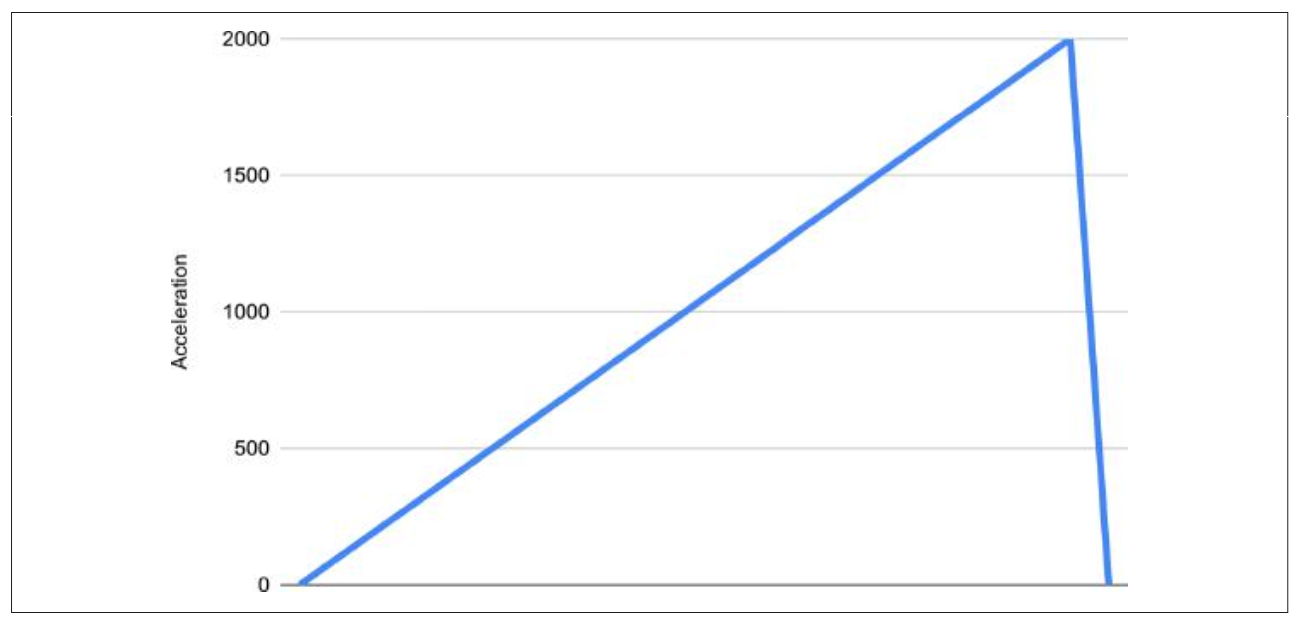
\includegraphics[width=\textwidth]{Images/Algorithm/Accelerometervalues1}
	\caption{\textbf{Accelerometer values for a single axis of a device being moved} \cite{Warden:2020}}
	\label{Fig:5.7}
\end{figure}

Each gesture is typically composed of a sequence of motions, with specific patterns in the accelerometer readings. For example, a "wing" gesture involves alternating upward and downward movements, along with changes in the horizontal direction. Figure \ref{Fig:5.8} shows an example of accelerometer data during a "wing" gesture, measured in milli-Gs.

\begin{figure}[h!]
	\centering
	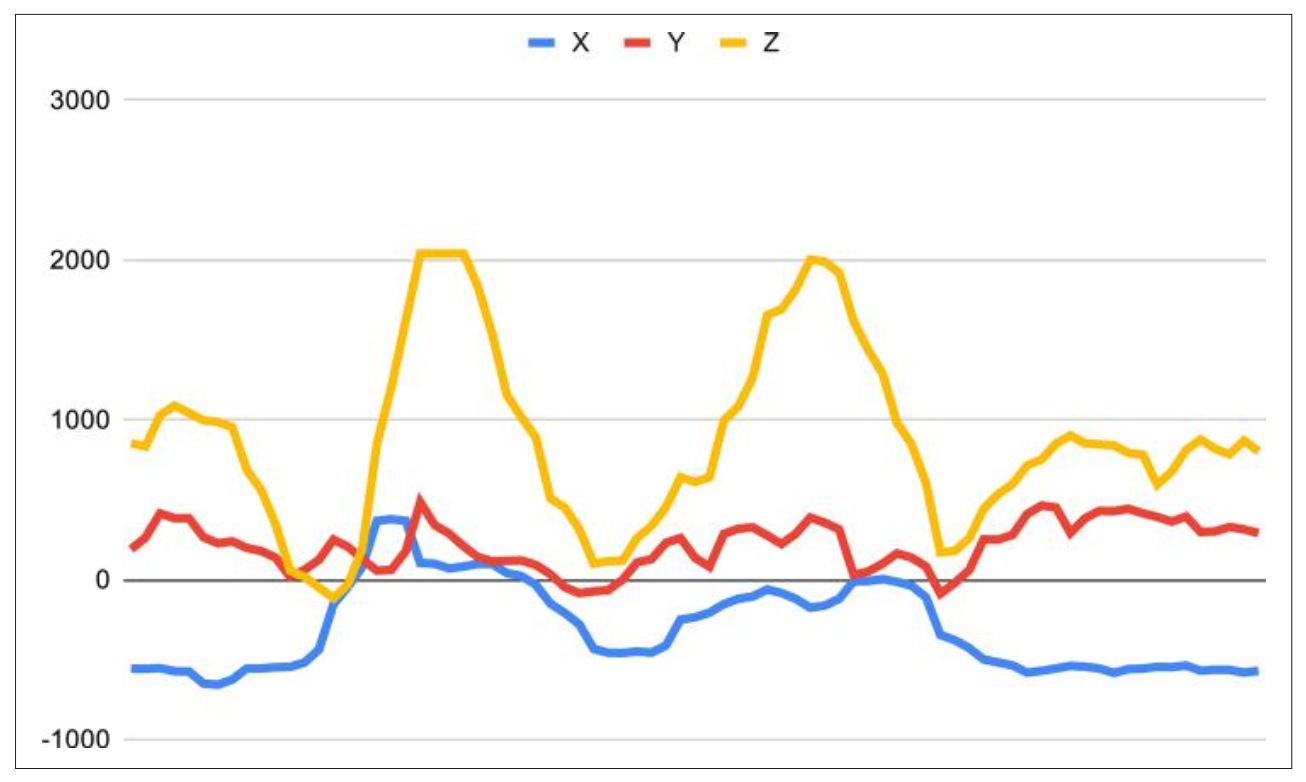
\includegraphics[width=\textwidth]{Images/Algorithm/Accelerometervalues2}
	\caption{\textbf{Accelerometer values during the “wing” gesture} \cite{Warden:2020}}
	\label{Fig:5.8}
\end{figure}

The accelerometer data consists of changes along the X, Y, and Z axes. By analyzing the relationship between these axes, a CNN can learn to identify specific gestures. For instance, the Z-axis acceleration might indicate up-and-down motion, while the X-axis acceleration can represent horizontal movement. The combination of these patterns helps identify the gesture being performed.

To achieve this, the CNN employs multiple layers of filters. Each filter learns to detect specific features within the data. For example, a filter in the first layer of the network might learn to detect upward acceleration, while a second layer might combine these detections to identify more complex features, such as the "wing" shape of the gesture. As the data progresses through the layers, simple patterns are combined into more complex structures, enabling the network to recognize gestures with high accuracy.

This process allows the CNN to learn from the noisy and raw input data, gradually transforming it into a high-level symbolic representation. At the final layers of the network, the symbolic representation is analyzed to predict the specific gesture being performed.

\section{Conclusion}

By using time-series accelerometer data as input, combined with the power of Convolutional Neural Networks, the Magic Wand Project can achieve accurate gesture recognition. The ability of CNNs to learn hierarchical feature representations from multidimensional input data makes them particularly effective for tasks involving motion and gesture analysis.

\section{Output}

The layer is configured with a "softmax" activation function \ref{Softmax Function}, which results in the layer’s output being a set of probabilities that sum to 1. This output is what we see in the model’s output tensor \ref{Fig:5.9} \ref{Fig:5.10} \ref{Fig:5.11}.

This type of model architecture—a combination of convolutional and fully connected layers—is very useful in classifying time-series sensor data like the measurements we obtain from our accelerometer. The model learns to identify the high-level features that represent the “fingerprint” of a particular class of input. It’s small, runs fast, and doesn’t take long to train. This architecture will be a valuable tool in your belt as an embedded machine learning engineer \cite{Warden:2020}.

\begin{center}
	\begin{tikzpicture}
		% define point
		\coordinate (A)  at (1, 1);
		\coordinate (O)  at (2, 0);
		\coordinate (B)  at (3, 1);
		\coordinate (C)  at  (4,0);
		\coordinate (D) at  (5,1);
		% angle  
		\draw[thick] (A) -- (O) -- (B) -- (C)-- (D);
		\draw [->, very thick] (1,1) -- (2,0)  node [midway, above] {\scriptsize };
		\draw [->, very thick] (2,0) -- (3,1)  node [midway, above] {\scriptsize };
		\draw [->, very thick] (3,1) -- (4,0)  node [midway, above] {\scriptsize };
		\draw [->, very thick] (4,0) -- (5,1)  node [midway, above] {\scriptsize };
	\end{tikzpicture}
	\captionof{figure}{\textbf{Wing Gesture}}
	\label{Fig:5.9}
\end{center}

\begin{figure}[H]\centering
	\begin{tikzpicture}
		\draw[->,very thick] (0,0) arc[radius=1cm,start angle=0,delta angle=359];
	\end{tikzpicture}
	\captionof{figure}{\textbf{Ring Gesture }}
	\label{Fig:5.10}
\end{figure}

\begin{figure}[H]\centering
	\begin{tikzpicture}
		% define point
		\coordinate (A)  at (2, 2);
		\coordinate (O)  at (0, 0);
		\coordinate (B)  at (2, 0);
		% angle  
		\draw[thick] (A) -- (O) -- (B);
		\draw [->, very thick] (2,2) -- (0,0)  node [midway, above] {\scriptsize };
		\draw [->, very thick] (0,0) -- (2,0)  node [midway, above] {\scriptsize };
	\end{tikzpicture}
	\captionof{figure}{\textbf{Slope Gesture }}
	\label{Fig:5.11}
\end{figure}

\subsection{Regression}

In a regression task, the CNN output is a continuous numerical value. The network is designed to predict a specific numerical outcome, and the final layer often uses an activation function, such as linear, that allows for unbounded output. The training process involves minimizing the difference between the predicted value and the actual target value, as determined by the chosen loss function \cite{Xu:2022}.

\subsection{Output of the Model for Magic Wand}
\label{subsection:outputCNN}

The CNN functions as a classifier, producing class probabilities as its output. The final outcome is determined by the softmax layer \ref{Softmax Function}, resulting in a set of numerical values corresponding to different gesture categories. For example, if the magic wand project involves recognizing gestures like "swirl," "tap," "circle," and "wave," the model might output probabilities such as \texttt{[0.05, 0.70, 0.10, 0.15]}.

Each number in the output array represents the model's confidence score for a specific gesture category, and the category with the highest score is considered the model's prediction for the given input gesture. In the provided example, the model predicts that the gesture category "tap" is the most likely result with a confidence score of 0.70.

To enhance the reliability of gesture recognition, postprocessing techniques can be applied. Methods like score averaging or consensus-based recognition are commonly used. Averaging scores over multiple runs contributes to a more stable and consistent output, improving the model's ability to adapt to variations in gesture patterns and environmental conditions \cite{Warden:2020}.

Upon successful recognition of a gesture, the magic wand's command responder can utilize the device's output capabilities, triggering actions such as changing LED colors, producing sounds, or initiating specific functions. The two-dimensional structure of the model's output, aligning with the first dimension as a wrapper and the second holding probabilities for each gesture class, is designed to suit the requirements of the embedded hardware implementation on Arduino Nano 33 BLE Sense \cite{Zhu:2019}.

\subsubsection{The Softmax Function}
\label{Softmax Function}
The softmax function is commonly used in Convolutional Neural Networks (CNNs) and other machine learning models, particularly in the output layer, to convert a vector of raw scores or logits into probabilities. It essentially normalizes the input values into a probability distribution that sums to 1 \cite{Sewak:2018}.

In the context of CNNs, the softmax function is often applied to the output layer when the network is used for classification tasks. Here's the formula for the softmax function:

\begin{equation}
	\text{Softmax}(x_i) = \frac{e^{x_i}}{\sum_{j=1}^{K} e^{x_j}}
\end{equation}

Where \( x_i \) is the raw score or logit for class \( i \), \( K \) is the total number of classes, and \( e \) is the base of the natural logarithm (Euler's number). An example of applying the Softmax function is shown in Figure \ref{fig:softmax}.

\begin{figure}[h!]
	\centering
	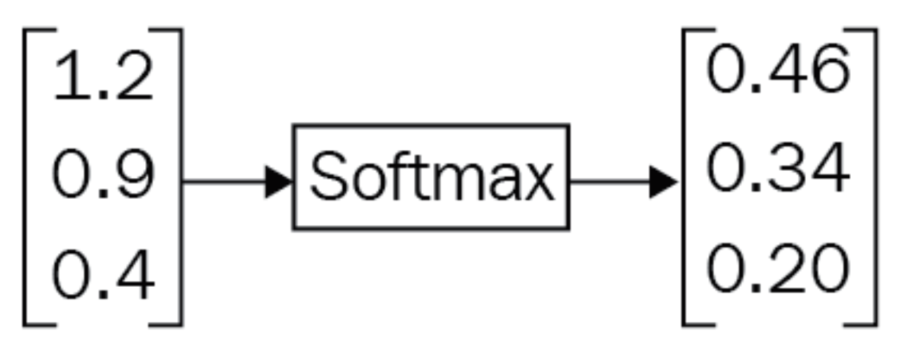
\includegraphics[width=0.4\textwidth]{Images/Algorithm/softmax}
	\caption{Example of applying the softmax function \cite{Sewak:2018}} \label{fig:softmax}
\end{figure}

\section{Python Example Code}
\label{section:AlgorithmExampleCode}


The identification of regional patterns within an image is facilitated by the convolutional layer. Following the convolutional layer, the max pooling layer is employed to diminish dimensionality. This section illustrates image classification by using a code provided by Sewak et al \cite{Sewak:2018}.

It is crucial to initially standardize all images to a uniform size. The initial convolution layer necessitates an additional parameter, \PYTHON{input.shape()}. The focus here is on training a Convolutional Neural Network (CNN) for image classification using the CIFAR-10 database. CIFAR-10 comprises 60,000 color images, each of size $32 \times 32$. These images are categorized into 10 classes, with 6,000 images per category, namely airplane, automobile, bird, cat, dog, deer, frog, horse, ship, and truck.

\subsection{Imports}

In the Listing \ref{code:cnnImports} are the necessary libraries and modules required for working with neural networks, image data, and visualization. The versions are shown in the Table \ref{tab:cnnlibraryVersions}.

\begin{itemize}
	\item Python version: 3.9.
\end{itemize}

\begin{table}[htbp]
	\centering
	\caption{Versions of Libraries}
	\label{tab:cnnlibraryVersions}
	\begin{tabular}{|l|c|}
		\hline
		\textbf{Library} & \textbf{Version} \\
		\hline
		Numpy & 1.23.5 \\
		Matplotlib & 3.7.1 \\
		Keras & 2.12.0 \\
		\hline
	\end{tabular}
\end{table}

\begin{code}[h!]
	\lstinputlisting[style=pythonstyle, numbers=none, linerange={82-89}]{Code/CNN/CNNDataMining.py}    
	\caption{Importing necessary libraries and modules.}
	\label{code:cnnImports}
\end{code}


\subsection{Load CIFAR-10 Dataset}

In Listing \ref{code:cnnLoadCifar} the CIFAR-10 dataset is loaded.CIFAR-10 is a dataset of 50,000 $32 \times 32$ color training images and 10,000 test images.

\begin{code}[h!]
	\lstinputlisting[style=pythonstyle, numbers=none, linerange={107-107}]{Code/CNN/CNNDataMining.py}    
	\caption{Loading and preparing the CIFAR-10 dataset.}
	\label{code:cnnLoadCifar}
\end{code}

\subsubsection{Data Preprocessing}

In the Listing \ref{code:cnnDataPreprocessing} the image data is normalized and one-hot encoding is performed on the labels. The training set is split into training and validation sets.

\begin{code}[h!]
	\lstinputlisting[style=pythonstyle, numbers=none, linerange={124-133}]{Code/CNN/CNNDataMining.py}    
	\caption{Preprocessing data: normalization, one-hot encoding, and splitting into training and validation sets}
	\label{code:cnnDataPreprocessing}
\end{code}

\subsection{Augmented Image Generator}

In the Listing \ref{code:cnnAugmentedGenerator} image data generators for training and validation is created and configured. These generators will perform data augmentation, such as shifting and flipping, to increase the diversity of the training set.

\begin{code}[h!]
	\lstinputlisting[style=pythonstyle, numbers=none, linerange={154-168}]{Code/CNN/CNNDataMining.py}    
	\caption{Configuring image data generators for augmentation and fitting them on training and validation data}
	\label{code:cnnAugmentedGenerator}
\end{code}

\subsection{Plot the First Nine Images of Cifar-10}

Listing \ref{code:cnnPlotCifar10} loads the cifar-10 dataset and plots the first nine images as shown in Figure \ref{fig:cnnFirstNineCifar10}.

\begin{code}[h!]
	\lstinputlisting[style=pythonstyle, numbers=none, linerange={177-183}]{Code/CNN/CNNDataMining.py}    
	\caption{Loading and visualizing the first nine images from the CIFAR-10 dataset}
	\label{code:cnnPlotCifar10}
\end{code}


\begin{figure}[h!]
	\centering
	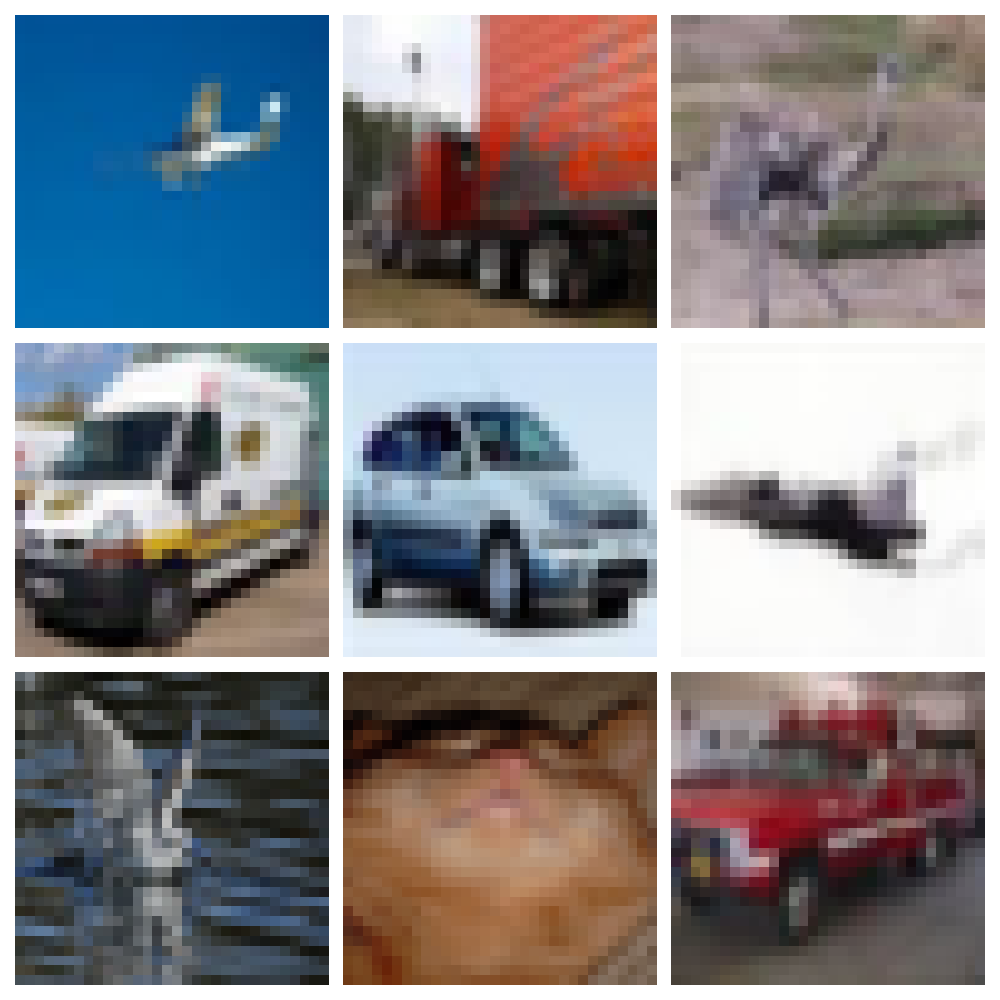
\includegraphics[width=0.8\textwidth]{Images/Algorithm/CIFAR10SecondNineImages}
	\caption{First nine images from the CIFAR-10 dataset.} \label{fig:cnnFirstNineCifar10}
\end{figure}

\subsection{CNN Model Definition}

A Convolutional Neural Network (CNN) model is defined in Listing \ref{code:cnnDefinition} using Keras with convolutional layers, max pooling, dropout for regularization, and dense layers.

\begin{code}[h!]
	\lstinputlisting[style=pythonstyle, numbers=none, linerange={199-207}]{Code/CNN/CNNDataMining.py}    
	\caption{Defining a Convolutional Neural Network (CNN) model using Keras}
	\label{code:cnnDefinition}
\end{code}

\subsection{Compile the Model}

In Listing \ref{code:cnnCompileModel} the model is compiled with the specified loss function, optimizer, and evaluation metric.

\begin{code}[h!]
	\lstinputlisting[style=pythonstyle, numbers=none, linerange={223-223}]{Code/CNN/CNNDataMining.py}    
	\caption{Compiling the CNN model with specified loss function, optimizer, and metric}
	\label{code:cnnCompileModel}
\end{code}

\subsection{Train the Model with Augmented Data}

In Listing \ref{code:cnnTrainAugmented} the model is trained using the augmented data generators. This involves calling the \PYTHON{fit\_generator} function instead of \PYTHON{fit} and providing the data generators for training and validation sets.

\begin{code}[h!]
	\lstinputlisting[style=pythonstyle, numbers=none, linerange={238-247}]{Code/CNN/CNNDataMining.py}    
	\caption{Training the CNN model with augmented data using data generators}
	\label{code:cnnTrainAugmented}
\end{code}


\subsection{Plotting the Loss and Accuracy Curves}

In Listing \ref{code:cnnLossAccuracyPlot} the accuracy and loss curves are plotted. The results are shown in the Figure \ref{fig:AccuracyandLoss}. The observed trends in the training and validation metrics, with a downward trend in both training and validation loss and an upward trend in accuracy, indicate positive learning and generalization behavior of the neural network. The somewhat unconventional scenario of validation loss being below training loss and validation accuracy exceeding training accuracy could be influenced by effective data augmentation, contributing to the model's robustness. These trends collectively suggest that the model is not overfitting the training data and is likely to generalize well to unseen data, highlighting successful training and potential for further improvement.

\begin{code}[h!]
	\lstinputlisting[style=pythonstyle, numbers=none, linerange={263-284}]{Code/CNN/CNNDataMining.py}    
	\caption{Plotting the loss and accuracy curves}
	\label{code:cnnLossAccuracyPlot}
\end{code}

\begin{figure}[h!]
	\centering
	
	\begin{subfigure}{0.45\textwidth}
		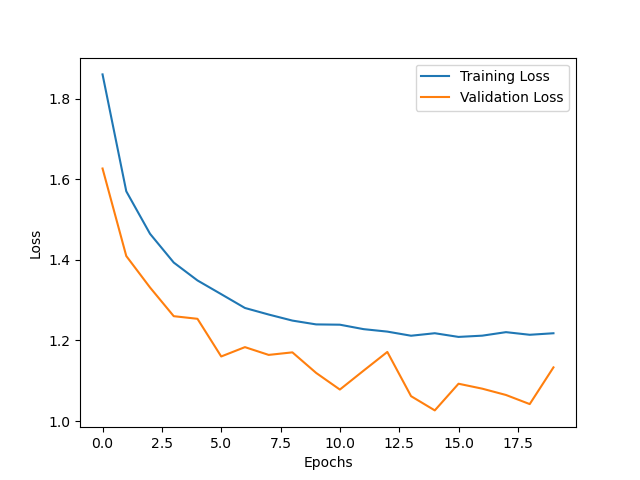
\includegraphics[width=\linewidth]{Images/Algorithm/lossPlot}
		\caption{}    % \caption{} is kept to keep (a), (b), (c) etc. below each subfigure.
		\label{subfig:lossTrends}
	\end{subfigure}
	\hfill
	\begin{subfigure}{0.45\textwidth}
		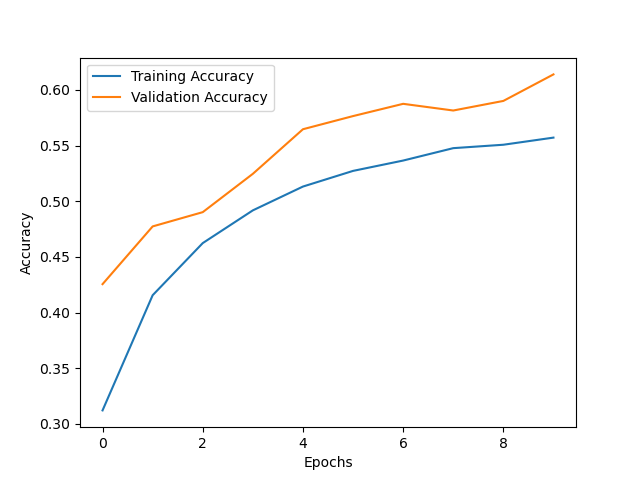
\includegraphics[width=\linewidth]{Images/Algorithm/accuracyPlot}
		\caption{}    % \caption{} is kept to keep (a), (b), (c) etc. below each subfigure.
		\label{subfig:accuracyTrends}
	\end{subfigure}
	
	\caption{(\subref{subfig:DigitalImage}) Training and validation loss trends over epochs. (\subref{subfig:DigitalImagePixelValues}) Training and validation accuracy trends over epochs.}
	\label{fig:AccuracyandLoss}
\end{figure}



\part{Development}
%%%%%%%%%%%%%%%%%%%%%%%%%%%%%%%%%%%%%%%%%%%%%
%
% $Autor: Adhiraj Walse Sudeshna Nanda Srikanth $
% $Datum: 2020-02-24 14:30:26Z $
% $Pfad: ML23-06-Magic-Wand-with-an-Arduino-Nano-33-BLE-sense/report/MagicWand.tex  $
% $Version: 1 $
%
% !TeX encoding = utf8
% !TeX root = NiclaVision
% !TeX TXS-program:bibliography = txs:///bibtex
%
%
%%%%%%%%%%%%%%%

\chapter{Development Environment}
\label{chapter 5}


\section{Arduino IDE Description}\label{ArduinoIDE}

It is an open source official Arduino software which used for editing, uploading and
compiling codes in to the Arduino module. It is a cross-platform software which is
available for Operating Systems like Windows, Linux, macOS. It runs on Java platform
and supports a range of Arduino modules. It supports C and C++ languages. The
microcontrollers present on the Arduino boards are programmed which accepts the
information in the form of code. The program written in the IDE is called a sketch
which will generate a Hex file which is then transferred and uploaded in the controller.
The IDE environment is made up of two parts: an editor and a compiler. The editor
is used to write the required code, while the compiler is used to compile and upload
the code to the Arduino Module.\cite{fezari:2018}
The Menu bar has options such as File in which there are many options including
Opening a new file or existing, Examples-in which we can find sketches for different
applications like Blink, Fade etc. There is an error console at the bottom of the screen
for displaying errors.

The 6 buttons are present on top of the screen are as follows:

\begin{figure}[H]\centering
	
\includegraphics[width=8cm]{Images/Development Environment/ArduinoIcons}
	\caption{\textbf{Menu button.}}
	\label{fig::ArduinoIDEmenubar}		
\end{figure}


\begin{itemize}
	\item	The check mark is used to verify your code. Click this once you have written your code.
	\item	The arrow uploads your code to the Arduino to run.
	\item	The dotted paper will create a new file.
	\item	The upward arrow is used to open an existing Arduino project.
	\item	The downward arrow is used to save the current file.
	\item	The far right button is a serial monitor, which is useful for sending data from the Arduino to the PC for debugging purposes.
\end{itemize}
\subsection{Installation}
\label{Arduinoide}
To install the Arduino IDE, we need to download the latest version from the Arduino webpage \url{https://www.arduino.cc/en/software}. We can select the version based on the operating system we are using. Here we are installing Arduino 1.8..15 for a Windows 10 operating system. 
The set up file name is arduino-1.8.15-windows.exe and the size of it is 1,17,470 KB. we can specify the path according to our needs. Here the path is set as  \SHELL{C:/Program Files (x86)/Arduino}.
\begin{figure}[H]\centering
	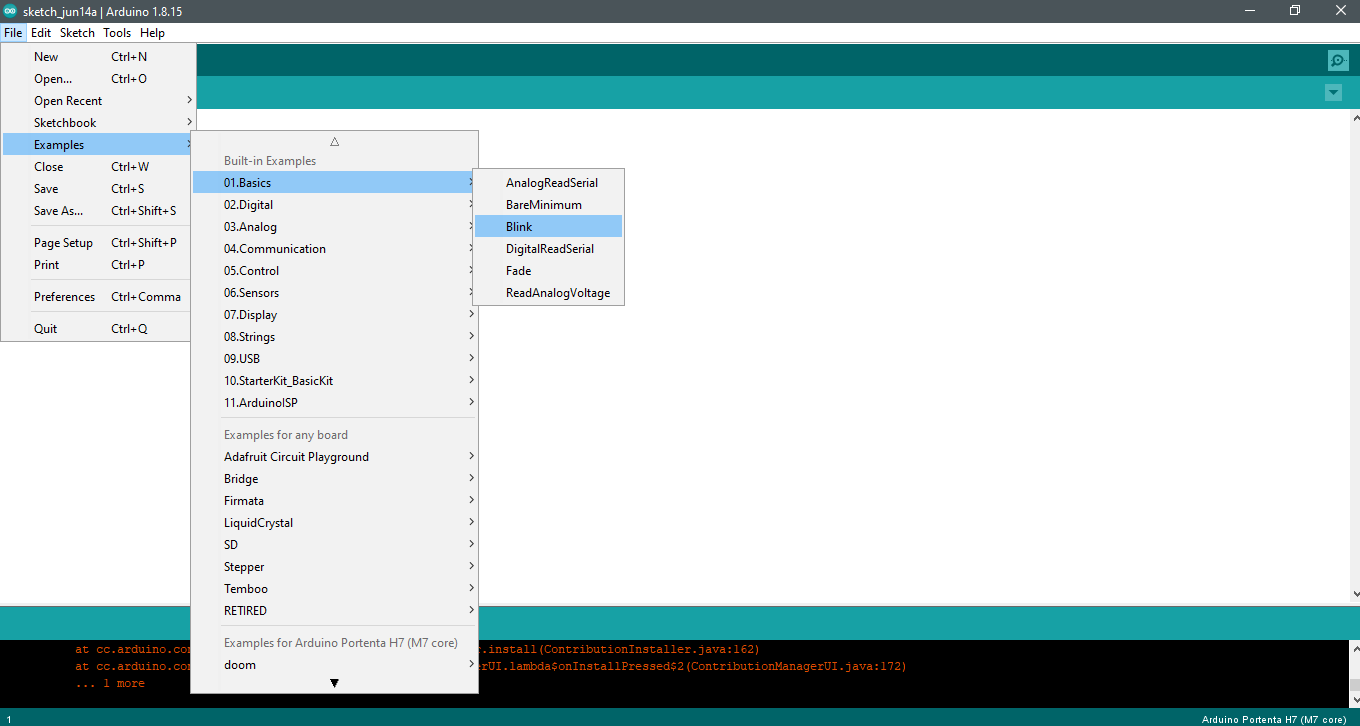
\includegraphics[width=8cm]{Images/Development Environment/Menu bar options}
	\caption{\textbf{Menu bar options.}}
	\label{fig::Menu bar options}		
\end{figure}
After the download is done, open the setup file and proceed to install.
Select all the components in the dialog box and click Next.\\

\begin{figure}[H]\centering
	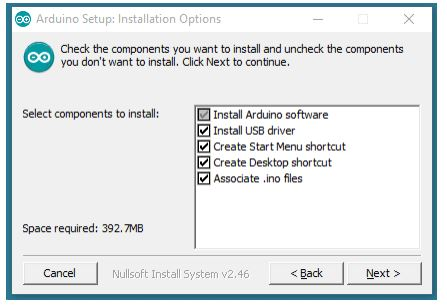
\includegraphics[width=8cm]{Images/Development Environment/Arduino Setup Installation options}
	\caption{\textbf{Arduino Setup Installation options.}}
	\label{fig:Arduino Setup Installation options}		
\end{figure}

Select the destination folder and click Install

\begin{figure}[H]\centering
	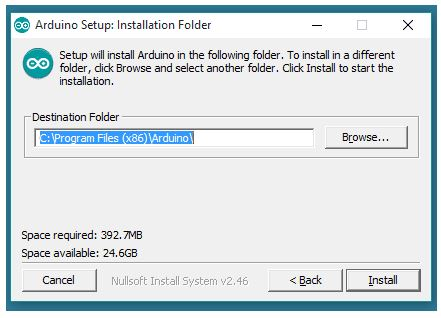
\includegraphics[width=8cm]{Images/Development Environment/Arduino Setup Installation Folder}
	\caption{\textbf{Arduino Setup Installation Folder.}}
	\label{fig:Arduino Setup Installation Folder}		
\end{figure}

Once the installation is done, open the Arduino IDE and a default sketch appears on the screen as shows.

\begin{figure}[H]\centering
	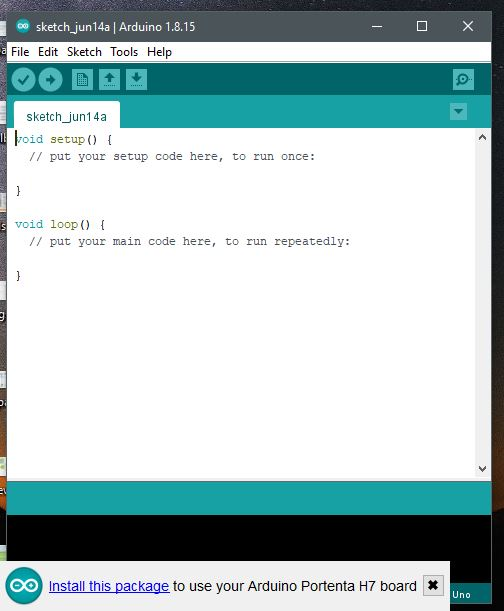
\includegraphics[width=8cm]{Images/Development Environment/Arduino Sketch}
	\caption{\textbf{Arduino Sketch.}}
	\label{fig:Arduino Sketch}		
\end{figure}


It can be seen from the above figure that the basic arduino sketch has two parts. The first part is the function \PYTHON{void setup()} which returns void and we do the intiliaztion such as the output LED color, specifying the core etc. The second part is the function \PYTHON{void loop()} where we define functions which are to be performed through out the loop. These codes are placed between paranthesis \PYTHON{$\{ \}$} and each function has a return type, here it has void return type.



\subsection{Arduino IDE on PC}
\subsubsection{Installation}
Arduino Nano 33 BLE Sense uses the Arduino software integrated development environment (IDE) for programming, which is the most widely used and common (IDE) for all arduino boards that can be run online and offline. This is a open-source Arduino Software (IDE) makes it easy to write code and upload it to the board. There are various version of software which is supported for each operating system (OS) e.g: mac, linux, and windows. Arduino community also provide us to start coding online and save our sketches in the cloud, this online arduino editor is most up-to-date version of the IDE includes all libraries and also supports new Arduino boards. For getting access to these software packages go to the following link \url{https://www.arduino.cc/en/software}  and get more up to date inforamtion, because every single day there are some updates occurs which is available on the link mention above. These software can be used with any Arduino board, the most recent offline arduino IDE 1.8.15 can be seen in Figure,\ref{fig:Arduino Creat Agent Installation}. it is also supportive for all operating systems.


\begin{figure}[H]\centering
	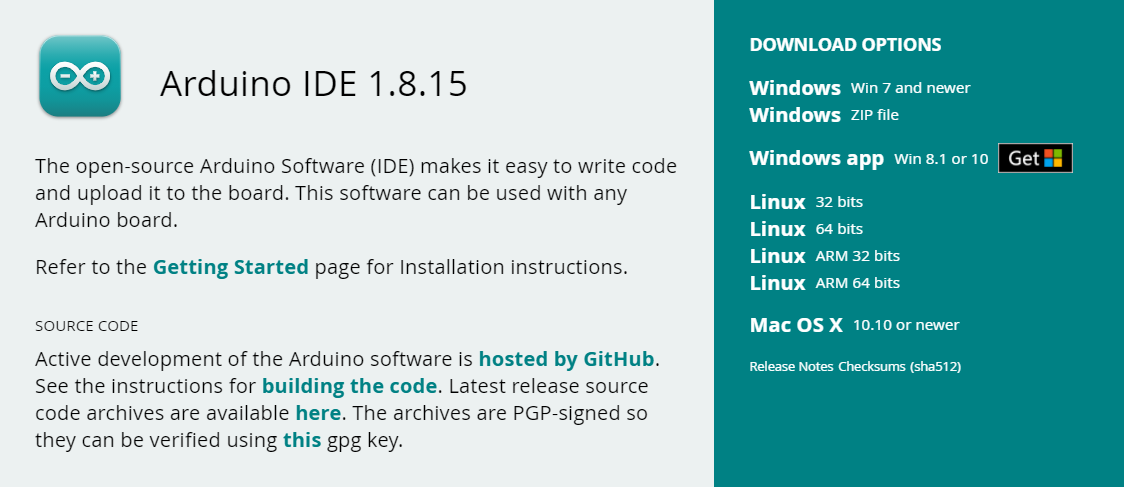
\includegraphics[width=8cm]{Images/Development Environment/Arduino Creat Agent Installation}
	\caption{\textbf{Arduino Creat Agent Installation.}}
	\label{fig:Arduino Creat Agent Installation}		
\end{figure}

\subsection{Configuration}
\subsubsection{Configuration for the Arduino Nano 33 BLE Sense}
To program the Arduino Nano 33 BLE Sense in offline state, we need to install one
of the latest arduino IDE on our desktop. After installation, for getting access to
the Arduino nano 33 ble sense board, we need to make configuration in our IDE. By
opening the IDE, go to tool which can be seen on the uper left corner in IDE, in the
tool there is an option for managed board. At this point we need to write our board
name in the search which is Arduino Nano 33 BLE Sense as shown in figure,\ref{fig:Arduino Mbed OS Nano Boards Installation}.Select
the Arduino Mbed OS Boards and install it. The Mbed OS nano board supports also
other nano family boards including Arduino nano 33 ble sense, after installing simply
connect the Arduino Nano 33 BLE Sense to the computer via USB cable.


\begin{figure}[H]\centering
	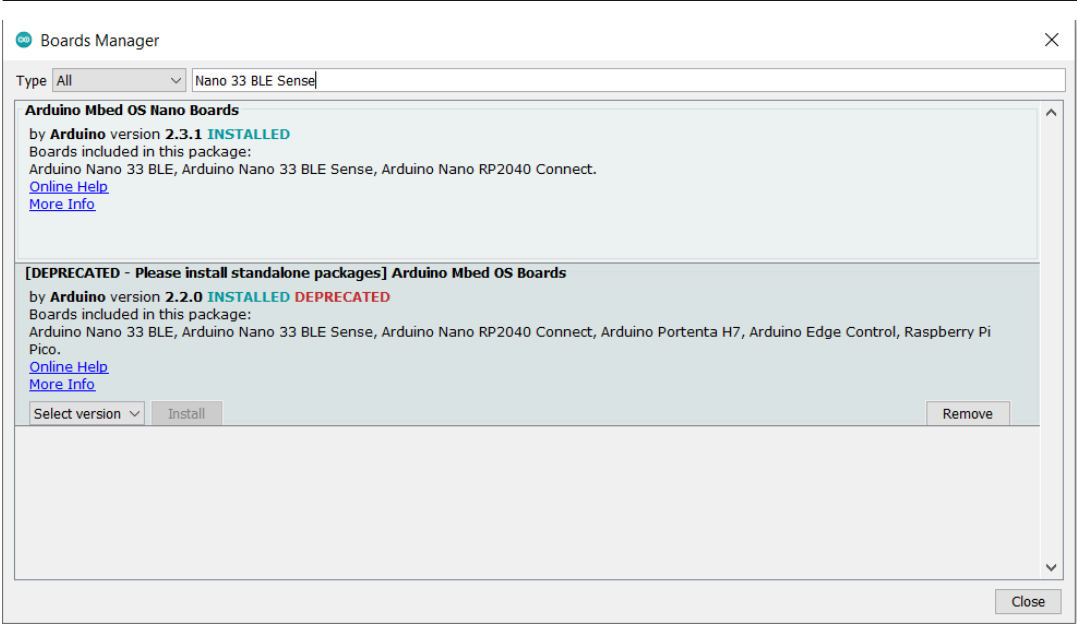
\includegraphics[width=8cm]{Images/Development Environment/Arduino Mbed OS Nano Boards Installation}
	\caption{\textbf{Arduino Mbed OS Nano Boards Installation.}}
	\label{fig:Arduino Mbed OS Nano Boards Installation}		
\end{figure}



\subsection{Setup}
There are set of examples which are build in Arduino (IDE) for the testing purpose, for checking all the configuration and setting up the board we can open one of the basic LED blink example first as shown in the figure.  \ref{fig:LED-Example Test}.



\begin{figure}[H]\centering
	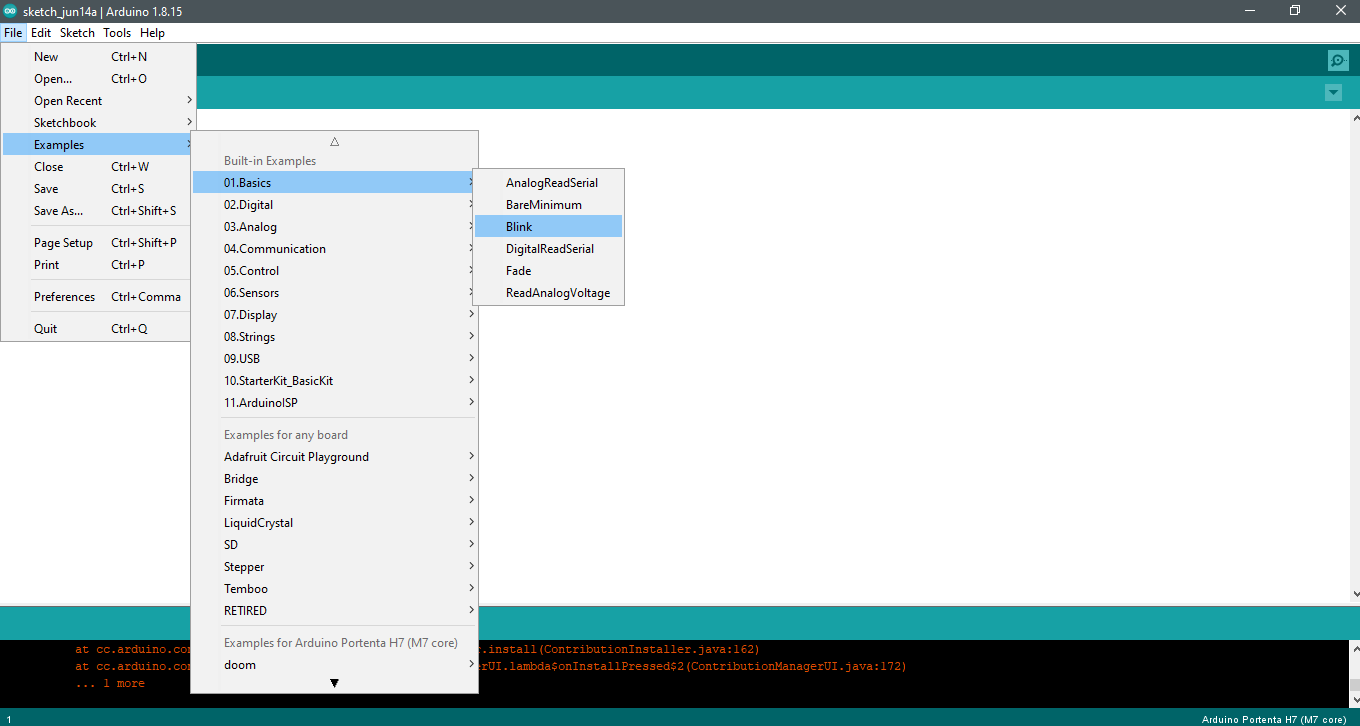
\includegraphics[width=8cm]{Images/Development Environment/Menu bar options}
	\caption{\textbf{LED-Example Test.}}
	\label{fig:LED-Example Test}		
\end{figure}
This LED-blink example support all the arduino boards, for the checking purposes just need to run this basic example on any arduino embed board and it will blink the LED on our Arduino board after pre-set miliseconds. In the same example folder, there are also number of build in usefull example written in Arduino IDE for embedded boards. These examples are very usefull for getting the basic knowledge about the board and programming.

\subsection{constraints}
There are some pre-requisite steps need to follow either we need to run the build in example or run by our own written program. By operating the Arduino board with Laptop with the help of USB connection, need to open the Arduino IDE on desktop, it appears a blank arduino environment page just a Void setup and void loop written on it. At this step we need to go to the tool-Arduino board and select the connected board which is Arduino Nano 33 Ble Sense as shown in the figure   \ref{fig:Select the Connected board -here Arduino Nano 33 BLE Sense}

\begin{figure}[H]\centering
	\includegraphics[width=8cm]{Images/Development Environment/Select the Connected board -here Arduino Nano 33 BLE Sense}
	\caption{\textbf{Select the Connected board -here Arduino Nano 33 BLE Sense.}}
	\label{fig:Select the Connected board -here Arduino Nano 33 BLE Sense}		
\end{figure}
\subsubsection{Select the Appropriate Port}
By selecting the Arduino nano 33 BLE sense board, next we need to check the connected port. For doing this, we need to set our arduino borad in Boot setup by clicking the white reset button on arduino as show in figure \ref{fig:Arduino Nano 33 BLE Sense Reset Button}

\begin{figure}[H]\centering
	\includegraphics[width=8cm]{Images/Development Environment/Arduino Nano 33 BLE Sense Reset Button}
	\caption{\textbf{Arduino Nano 33 BLE Sense Reset Button.}}
	\label{fig:Arduino Nano 33 BLE Sense Reset Button}		
\end{figure}
By clicking the white reset button, the arduino borad will be in boot setup and make
sure to check the orange LED glows as shown in the figure\ref{fig:Arduino Nano 33 BLE Sense Orange LED Glow}
\begin{figure}[H]\centering
	\includegraphics[width=8cm]{Images/Development Environment/Arduino Nano 33 BLE Sense Orange LED Glow}
	\caption{\textbf{Arduino Nano 33 BLE Sense Orange LED Glow.}}
	\label{fig:Arduino Nano 33 BLE Sense Orange LED Glow}		
\end{figure}
After successfully applying the above mention step, next we need to select the connected
port before upload the program. For this, go to tool select arduino port and make
sure to check it available port for uploading the program as shown in figure\ref{fig:Select Available Port for Uploading Arduino Sketch}
\begin{figure}[H]\centering
	\includegraphics[width=8cm]{Images/Development Environment/Select Available Port for Uploading Arduino Sketch}
	\caption{\textbf{Select Available Port for Uploading Arduino Sketch.}}
	\label{fig:Select Available Port for Uploading Arduino Sketch}		
\end{figure}

\subsubsection{Upload Code in Arduino Board}\label{uploadcode}
By making sure to select the appropriate port, it’s time to upload the Arduino program.
There are five icons (verify, upload, new, open, save) below the file section, before
uploading the program the best practice is to verify the program first, it show us if
there are any error or warning in the program exist or not. By successfully verifying
the program we can safely upload the program by click the upload button in the top
below the file section as shown in figure.\ref{fig:Upload the Program in Arduino board}
\begin{figure}[H]\centering
	\includegraphics[width=8cm]{Images/Development Environment/Upload the Program in Arduino board}
	\caption{\textbf{Upload the Program in Arduino board.}}
	\label{fig:Upload the Program in Arduino board}		
\end{figure}
After uploading, the code will compile and if there is any issue in our program it will
pop up in the bottom black window as well.
After successfully uploading and compiling the code in Arduino board, it also require
to change the port again as we did it previously. Go to tool select arduino port and
make sure to check the port again as shown in figure\ref{fig:Setting the Port} by getting output in the
serial monitor.
\begin{figure}[H]\centering
	\includegraphics[width=8cm]{Images/Development Environment/Setting the Port}
	\caption{\textbf{Setting the Port.}}
	\label{fig:Setting the Port}		
\end{figure} 
\subsection{Conclusions}
\subsubsection{Output Window (Serial Monitor)}
Serial Monitor is the another window on the Arduino IDE, which shows the Input/Output of our program and results appear on it as per the required output. For getting
access to Serial monitor, we need to go extreme right in the Arduino IDE, the small
circle pop up when we reach it is the serial monitor as show in the figure.\ref{fig:Serial Monitor Icon}
\begin{figure}[H]\centering
	\includegraphics[width=8cm]{Images/Development Environment/Serial Monitor Icon}
	\caption{\textbf{Serial Monitor Icon.}}
	\label{fig:Serial Monitor Icon}		
\end{figure} 
The Final results, all the variables, input, sensor values are shown in the serial monitor
the (Output Window) as shown in the figure\ref{fig:Output Window} by clicking the serial monitor button.
\begin{figure}[H]\centering
	\includegraphics[width=8cm]{Images/Development Environment/Output Window}
	\caption{\textbf{Output Window.}}
	\label{fig:Output Window}		
\end{figure} 


\section{TensorFlow}
\label{TensorFlow}

\ac{tf} is an end-to-end, open-source platform popularly used for the quick implementation of machine learning algorithms. A rich ecosystem of tools, libraries, and community resources has made it extremely popular among machine learning researchers and practitioners to develop and deploy various machine learning algorithms with greater efficiency and flexibility. TensorFlow has become popular in recent times for the quick development of complex deep neural network architectures for both experimentation and developing production-ready software.\cite{TensorFlow:2023}

TensorFlow was originally developed by Google within their Machine Intelligence Research Organization to conduct various machine learning and neural networks related research. The initial version was released in 2015 under the Apache License 2.0. TensorFlow 2.0, the newest stable version, was released in 2019. TensorFlow is highly flexible. It supports a wide variety of programming languages, including Python, C++, and Java. Moreover, it can run on CPU, GPU, and TPU for a faster processing of large machine learning applications. TensorFlow is available in Linux, macOS X, and Windows platforms. It also supports TensorFlow Lite, a highly optimized lighter version of the original TensorFlow that is available on mobile computing platforms such as Android, iOS-based smartphones, and Linux-based single board computers like Raspberry Pi. TensorFlow Lite models can be further optimized using a few standard APIs to run on microcontroller units. Hence, TensorFlow is heavily used in TinyML applications. Visit the official TensorFlow website for more details. To summarize, some of the key features of TensorFlow are as follows:

\begin{itemize}
	
	\item It is open-source 
	
	\item Efficiently works with multi-dimensional data
	
	\item Provides a higher level of abstraction, which reduces the code length for the developer 
	
	\item Supports various platforms and architectures
	
	\item Highly scalable and provides greater flexibility for quick prototyping 
	
\end{itemize}

\subsection{Installation}

TensorFlow, along with all its dependencies, is already installed in Colab. So, you just need to import the libraries to write codes without any package installation. TensorFlow can be imported by typing the following command in the code cell.


\begin{lstlisting}[language=Python, caption={Import TensorFlow and Check Version}, label={code:tensorflow-version}, style=pythonstyle]
	# Import TensorFlow
	import tensorflow as tf
	
	# Check TensorFlow version
	tf._version_
\end{lstlisting}


Once TensorFlow is imported, you can check the version by typing the command \textbf{tf.\_version\_}. At the time of writing this book, the TensorFlow version in Colab is 2.12.0, which may change with time. TensorFlow 2, or TF 2, is the newest version which is significantly different compared to the previous version TF 1.x. In this book, we will use TF2 for all our programming. However, TF 2 provides a backward compatibility module to use TF 1.x. The eager execution mode of TF 2 makes it easier to create a machine learning architecture with lesser lines of code. \cite{TensorFlow:2023} 


\subsection{constraints}

Once we are done with loading and pre-processing of the data, we can define neural network architecture.
A Keras model has the following four stags:

\begin{enumerate}
	
	\item Defining the model: We define a Sequential model and add the necessary layers.
	
	\item Compiling the model: We configure the model for training by defining the loss function to be minimized, the optimizer that minimizes the loss function, and a performance metric to internally evaluate the performance. 
	
	\item Fitting the model: Here, we fit the model on the actual training data for a given number of epochs to update the training parameters. We will get the model at the end of training.
	
	\item Evaluation: Once you have the model, you can evaluate on unseen test data
	
\end{enumerate}


\subsection{Conclusions}

One of the biggest benefits of using TensorFlow is the level of abstraction. It takes care of the major details of most of the underlying algorithms in a machine learning or a deep learning application, for example, backpropagation. Hence, writing programs in TensorFlow is super easy as you mostly need to focus on your application logic. TensorFlow applications can run on almost any target environment, such as local desktops, remote servers running Windows, Linux, macOS X, smartphone devices running Android and iOS, or Linux-based single board computers. TensorFlow contains additional libraries to convert a machine learning model into C++ equivalent libraries to run on selected microcontrollers. Hence, you can use TensorFlow to create your TinyML applications. Throughout this book, we will primarily use Keras to implement the machine learning models. Keras is a high-level set of Python \ac{api} in TensorFlow, which is popularly used in the rapid prototyping of various neural network models. Fortunately, both TensorFlow and Keras are readily available in Colab. So, you can easily start writing your program in Colab without installing any extra libraries. In this chapter, we will primarily focus on creating end-to-end neural network models using TensorFlow. The later chapters will focus on optimizing the neural networks to create deployable TinyML applications.


%\section{Conclusion}
%
%Python is a very popular programming language in machine learning for researchers and also for developing production-ready software. A good understanding of Python is a prerequisite to fully understand the rest of the topics covered in the book. This chapter has been designed as a crash course to brush up on your Python programming knowledge before moving to the more complex part of programming in deep learning and TinyML applications. We assume that the readers have some fundamental knowledge of Python programming. Those who require an in-depth knowledge of Python and its various libraries are strongly encouraged to read the various resources available in print and also in digital mediums. The readers should try to execute the examples covered in this book at their end and are also strongly encouraged to modify, tweak, and extend them to gain more confidence in writing their own codes independently.

%\section{Further reading}
%
%\begin{enumerate}
%	
%	\item \textbf{Beazley, David, and Brian K. Jones. Python cookbook: Recipes for mastering Python 3. "O'Reilly Media, Inc.", 2013.}
%	
%	This book provides a collection of practical and diverse Python recipes for mastering the language. It covers a wide range of topics and scenarios, offering solutions and insights that help developers become more proficient in Python programming.
%	
%	\item \textbf{Pajankar, Ashwin. "Introduction to Python." In Python Unit Test Automation, pp. 1-17. Apress, Berkeley, CA, 2017.}
%	
%	Introducing Python through the lens of unit testing, this book explains the fundamentals of Python and how to apply them to automate unit testing. It's a practical guide that combines Python programming with testing practices for software quality assurance.
%	
%	\item \textbf{Cutler, Josh, and Matt Dickenson. "Introduction to Machine Learning with Python." In Computational Frameworks for Political and Social Research with Python, pp. 129-142. Springer, Cham, 2020.}
%	
%	Embedded within a broader context of computational frameworks for social and political research, this book offers an introduction to machine learning concepts using Python. It explores the application of machine learning techniques in the realm of social and political research.
%	
%	\item \textbf{Joshi, Prateek. Artificial intelligence with Python. Packt Publishing Ltd, 2017.}
%	
%	Focused on artificial intelligence, this book provides insights into various AI techniques using Python. It covers topics like machine learning, natural language processing, and neural networks, guiding readers through the implementation of AI models.
%	
%	\item \textbf{Campesato, Oswald. TensorFlow 2 Pocket Primer. Stylus Publishing, LLC, 2019.}
%	
%	This concise primer delves into TensorFlow 2, a popular deep learning framework. It offers a quick reference for readers to understand and work with TensorFlow 2, covering essential concepts and techniques.
%	
%	\item \textbf{Singh, Pramod, and Avinash Manure. Learn TensorFlow 2.0: Implement Machine Learning and Deep Learning Models with Python. Apress, 2019.}
%	
%	Centered around TensorFlow 2.0, this book provides practical guidance on implementing machine learning and deep learning models using Python. It offers step-by-step examples and insights into various aspects of deep learning.
%	
%\end{enumerate}
%

\section{TensorFlow Lite}
To meet these lower size requirements for mobile platforms, in 2017 Google started a companion project to mainline TensorFlow called TensorFlow Lite. This library is aimed at running neural network models efficiently and easily on mobile devices. To reduce the size and complexity of the framework, it drops features that are less cons mon on these platforms. For example, it doesn't support training, just running infer ence on models that were previously trained on a cloud platform. It also doesn't support the full range of data types (such as double) available in mainline Tensor Flow Additionally, some less-used operations aren't present, like tf.depth\_to\_space You can find the latest compatibility information on the TensorFlow website.

In return for these trade-offs, TensorFlow Lite can fit within just a few hundred kilo- bytes, making it much easier to fit into a size-constrained application. It also has highly optimized libraries for Arm Cortex-A-series CPUs, along with support for Android's Neural Network API for accelerators, and GPUs through OpenGL Another key advantage is that it has good support for 8-bit quantization of networks Because a model might have millions of parameters, the 75\% size reduction from 32- bit floats to 8-bit integers alone makes it worthwhile, but there are also specialized code paths that allow inference to run much faster on the smaller data type.\cite{TensorFlow:2023}



\subsection{Installation}

\begin{lstlisting}[language=Python, caption={Load and Run TensorFlow Lite Model}, label={code:tflite-inference}, style=pythonstyle]
	import tensorflow as tf
	import numpy as np
	
	# Load the TensorFlow Lite model.
	interpreter = tf.lite.Interpreter(model_path="model.tflite")
	interpreter.allocate_tensors()
	
	# Get the input and output tensors.
	input_details = interpreter.get_input_details()
	output_details = interpreter.get_output_details()
	
	# Create some input data.
	input_data = np.array([[1.0, 2.0, 3.0]])
	
	# Set the input tensor.
	interpreter.set_tensor(input_details[0]["index"], input_data)
	
	# Perform inference.
	interpreter.invoke()
	
	# Get the output tensor.
	output_data = interpreter.get_tensor(output_details[0]["index"])
	
	# Print the output.
	print(output_data)
\end{lstlisting}


\subsection{constraints}

TensorFlow Lite for Microcontrollers is designed for the specific constraints of microcontroller development.\cite{TensorFlow:2023} If you are working on more powerful devices (for example, an embedded Linux device like the Raspberry Pi), the standard TensorFlow Lite framework might be easier to integrate The following limitations should be considered:

\begin{itemize}
	
	\item Support for a limited subset of TensorFlow operations.
	
	\item Support for a limited set of devices.
	
	\item Low-level C++ API requiring manual memory management.
	
	\item On device training is not supported
	
\end{itemize}

\subsection{Conclusions}
TensorFlow Lite is a lightweight version of TensorFlow, designed specifically for mobile and embedded devices. In the TinyML magic wand
project using Arduino Nano, TensorFlow Lite is used to run a pre-trained
machine learning model on the Arduino Nano board.
The magic wand project involves using a gesture recognition model
to detect different hand movements and control a small toy wand. The
Arduino Nano board is used to collect sensor data from an accelerometer
and gyro sensor, which is then fed into the machine learning model running
on the board. The model uses TensorFlow Lite to make predictions based
on the sensor data and determine what hand gesture is being made. Based
on the prediction, the wand can be controlled to perform different actions.
The use of TensorFlow Lite in this project allows the machine learning
model to run efficiently on the limited resources of the Arduino Nano
board. By using a lightweight model and optimizing the code for the
microcontroller architecture, it is possible to perform gesture recognition
on a low-power, low-cost device like the Arduino Nano. This makes the
project more accessible and affordable for hobbyists and students who
want to experiment with TinyML applications.\cite{Magicwand:2024}



\section{TensorFlow Lite for Microcontrollers}

\subsection{Introduction}

TensorFlow Lite has been widely adopted by mobile developers, but its engineering trade-offs didn't meet the requirements of all platforms. The team noticed that there were a lot of Google and external products that could benefit from machine learning being build on embedded platforms, on which the existing TensorFlow Lite library wouldn't fit. Again, the biggest constraint was binary size. For these environments even a few hundred kilobytes was too large; they needed something that would fit within 20 KB or less. A lot of the dependencies that mobile developers take for gran- ted. like the C Standard Library, weren't present either, so no code that relied on these libraries could be used. A lot of the requirements were very similar, though. Inference was the primary use case, quantized networks were important for performance, and having a code base that was simple enough for developers to explore and modify was a priority.\cite{TensorFlow:2023}

\subsection{Work Flow}

\begin{enumerate}
	
	\item Train a model:
	
	\begin{itemize}
		
		\item Generate a small TensorFlow model that can fit your target device and contains supported operations.
		
		\item Convert to a TensorFlow Lite model using the TensorFlow Lite converter.
		
		\item Convert to a C byte array using standard tools to store it in a read-only program memory on device.
		
	\end{itemize}
	
	\item Run inference on device using the C++ library and process the results.
	
\end{enumerate}
\subsection{Installation}

\begin{lstlisting}[language=C++, caption={Run Inference with TensorFlow Lite Micro}, label={code:tflite-micro-inference}, style=bashstyle]
	#include "model.h"
	#include "tensorflow/lite/micro/kernels/micro_ops.h"
	#include "tensorflow/lite/micro/micro_error_reporter.h"
	#include "tensorflow/lite/micro/micro_interpreter.h"
	#include "tensorflow/lite/version.h"
	
	// Create an instance of the error reporter
	static tflite::MicroErrorReporter micro_error_reporter;
	
	// Define the tensor arena
	static constexpr int kTensorArenaSize = 2 * 1024;
	static uint8_t tensor_arena[kTensorArenaSize];
	
	// Create an instance of the interpreter
	static tflite::MicroInterpreter static_interpreter(
	model, tflite::MicroOpResolver::GetDefault(), tensor_arena,
	kTensorArenaSize, &micro_error_reporter);
	
	// Allocate memory for the input and output tensors
	TfLiteTensor* input = static_interpreter.input(0);
	TfLiteTensor* output = static_interpreter.output(0);
	
	// Perform inference
	static_interpreter.Invoke();
	
	// Print the output
	for (int i = 0; i < output->bytes; i++) {
		printf("%f ", output->data.f[i]);
	}
\end{lstlisting}


\subsection{constraints}

Running in embedded environments imposed a lot of constraints on how the code could be written, so it identified some key requirements for the library:

\begin{enumerate}
	
	\item \textbf{No operating system dependencies}
	
	A machine learning model is fundamentally a mathematical black box where numbers are fed in, and numbers are returned as the results. Access to the rest of the system shouldn't be necessary to perform these operations, so it's possible to write a machine learning framework without calls to the underlying operating system. Some of the targeted platforms don't have an OS at all, and avoiding any references to files or devices in the basic code made it possible to port to those chips.\cite{War:2020}
	
	\item \textbf{No standard Cor C++ library dependencies at linker time }
	
	This is a bit subtler than the OS requirement, but the team was aiming to deploy on devices that might have only a few tens of kilobytes of memory to store a pro- gram, so the binary size was very important. Even apparently simple functions like sprintf() can easily take up 20 KB by themselves, so the team aimed to avoid anything that had to be pulled in from the library archives that hold the implementations of the C and C++ standard libraries. This was tricky because there's no well-defined boundary between header-only dependencies (like stdint.h, which holds the sizes of data types) and linker-time parts of the standard libraries (such as many string functions or sprintf().
	
	\item \textbf{No floating point hardware expected }
	
	Many embedded platforms don't have support for floating-point arithmetic in hardware, so the code had to avoid any performance-critical uses of floats. This meant focusing on models with 8-bit integer parameters, and using 8-bit arith metic within operations (though for compatibility the framework also supports float ops if they're needed). \cite{Ard:2021}
	
	\item \textbf{No dynamic memory allocation}
	
	A lot of applications using microcontrollers need to run continuously for months or years. If the main loop of a program is allocating and deallocating memory using malloc()/new and free()/delete, it's very difficult to guarantee that the heap won't eventually end up in a fragmented state, causing an allocation failure and a crash. There's also very little memory available on most embedded systems, so upfront planning of this limited resource is more important than on other platforms, and without an OS there might not even be a heap and allocation rou- tines. This means that embedded applications often avoid using dynamic memory allocation entirely. Because the library was designed to be used by those applications, it needed do the same. 
	
	In practice the framework asks the calling application to pass in a small, fixed-size arena that the framework can use for temporary allocations (like activation buffers) at initialization time. If the arena is too small, the library will return an error immediately and the client will need to recompile with a larger arena. Otherwise, the calls to perform inference happen with no further memory allocations, so they can be made repeatedly with no risk of heap fragmentation or memory errors.\cite{War:2020}
	
\end{enumerate}

\subsection{Conclusions}
In the TinyML magic wand project using Arduino Nano, TensorFlow Lite Micro is used to run a machine learning model on the Arduino Nano board to recognize gestures made with the wand. The model is trained to recognize a specific set of gestures (e.g., waving the wand up and down,
left and right) and can trigger different actions based on the recognized
gesture (e.g., turn on/off lights, play music).
Using TensorFlow Lite Micro on the Arduino Nano enables the wand
to perform gesture recognition locally on the device, without the need
for an internet connection or a more powerful computer. This makes the
wand more portable and flexible, and can be used in a wider range of
environments and applications.
Overall, TensorFlow Lite Micro enables the development of TinyML
(Tiny Machine Learning) applications that run on microcontrollers and other embedded devices, making it possible to bring machine learning
capabilities to a wide range of IoT and edge devices.\cite{Gomez:2012}

Our application will be deployed on Arduino Nano 33 BLE Sense, which is a recommended microcontroller board for TinyML applications. The application we are going to implement is fairly simple. The microcontroller will read the linearly varying electrical voltage provided by an external potentiometer as its input, convert the voltage values as per a halfwave sinusoid function using a simple neural network, and controls the brightness of an LED accordingly. Remember, due to its resource constraints, you cannot even train a small neural network on a microcontroller. We will train the neural network in Colab using TensorFlow, The model will be converted into a TFLite model. This part of the project will be implemented in Python. We will then convert the model into an equivalent C/C++ library for microcontrollers. Next, we will write an inference application for Arduino using a programming language that is very similar to C/C++. 

\section{Python}
The Arduino IDE is written only in C++ language and is not supported the other programming languages. Some of the Module I used specially for executing the Gesture detection part of this project is only support python language e.g., MediaPipe and OpenCV. MediaPipe and OpenCV module are the most important part for gesture detection, for detecting the landmarks on hand the supported function is written in python. Without the MediaPipe Module, the hand landmarks technique is not possible to implement. At the moment, there is no such module or library who can support directly MediaPipe Module in Arduino IDE and C++, because MediaPipe Module is written in python.\cite{Alk:2019}
\subsection{Installation}
\label{Python}
\begin{lstlisting}[language=Python, caption={Load and Run TensorFlow Lite Model}, label={code:tflite-inference-python}, style=pythonstyle]
	import tensorflow as tf
	import numpy as np
	
	# Load the TensorFlow Lite model.
	interpreter = tf.lite.Interpreter(model_path="model.tflite")
	interpreter.allocate_tensors()
	
	# Get the input and output tensors.
	input_details = interpreter.get_input_details()
	output_details = interpreter.get_output_details()
	
	# Create some input data.
	input_data = np.array([[1.0, 2.0, 3.0]])
	
	# Set the input tensor.
	interpreter.set_tensor(input_details[0]["index"], input_data)
	
	# Perform inference.
	interpreter.invoke()
	
	# Get the output tensor.
	output_data = interpreter.get_tensor(output_details[0]["index"])
	
	# Print the output.
	print(output_data)
\end{lstlisting}

\subsection{constraints}
Python, although versatile, has constraints in the context of the magic wand project with Arduino Nano 33 BLE. Real-time operations pose a challenge due to Python's lack of native support, potentially affecting precise timing for gesture recognition. Additionally, Python's interpreted nature may result in slower execution, impacting sensor data processing and model inference speed. Memory usage can be a concern on resource-constrained microcontrollers, like Arduino Nano. While Python is not inherently optimized for the lightweight requirements of such devices, developers can mitigate these constraints by employing efficient coding practices and considering alternatives for critical real-time tasks.


\subsection{Conclusion}
The use of Python in the software aspect of the magic wand project enhances flexibility, allowing for efficient data processing, machine learning model training, and seamless communication with the Arduino Nano 33 BLE.


\section{PyCharm}
\label{Pycharm}
PyCharm, a robust Python integrated development environment (IDE), plays a pivotal role in the software development process for the magic wand project with Arduino Nano. Leveraging PyCharm's advanced code editing and navigation features, the development team benefits from an efficient and organized coding experience. The IDE's support for project management, version control integration with Git, and seamless debugging and profiling tools contribute to a streamlined development workflow. PyCharm's capabilities extend to virtual environment support, ensuring effective dependency management for the machine learning aspects of the project. Additionally, PyCharm facilitates integration with continuous integration (CI) systems, enabling automated testing and build processes. Overall, PyCharm proves indispensable in enhancing code quality, collaboration, and the overall efficiency of the machine learning software development on the Arduino Nano platform.\cite{Learn:2021}
\subsection{Setup}
To install PyCharm, begin by visiting the official PyCharm website and downloading the appropriate version for your needs—Community (free) or Professional (paid). Run the installer, typically an executable file on Windows, and follow the on-screen instructions. Choose the installation location, edition, and any additional settings. If you opt for the Professional edition, activate a license during the installation or choose to evaluate it for a trial period. Once installed, run PyCharm, configure a Python interpreter, and start coding. It's advisable to consult the official PyCharm documentation for detailed and platform-specific instructions.
\subsection{constraints}
PyCharm, while a versatile and powerful integrated development environment (IDE) for Python, presents certain constraints that users should consider. One notable constraint is its resource intensiveness, potentially causing performance issues on machines with limited RAM or processing power, especially in larger projects. Additionally, the learning curve can be steep for new users due to the extensive feature set. Cost can be a constraint for users requiring advanced features in the professional version. Compatibility issues may arise with specific Python libraries or frameworks, and users should stay updated to avoid such constraints. While PyCharm is specialized for Python, its support for other languages may be limited. Plugin dependencies, heavy initial indexing for large projects, and constraints related to remote development or extremely complex projects further warrant consideration. Awareness of these constraints empowers users to make informed decisions based on their development needs and project characteristics.
\subsection{Conclusion}
PyCharm serves as an integral component of the development toolkit for the magic wand project with Arduino Nano. Its comprehensive set of features enhances the coding experience, fosters collaboration, and contributes to the overall efficiency of the software development process.\cite{Learn:2021}

\section{Github}
The Github repository for the "Magic Wand with Arduino Nano 33 BLE" project comprises key components essential for its development and usage. The heart of the project lies in the Arduino code, intelligently crafted to collect sensor data, interact seamlessly with TensorFlow Lite, and execute actions based on machine learning predictions. This codebase is housed within the dedicated arduino code directory, providing a clear organization of the software responsible for the wand's functionality.
%%%%%%%%%%%%
%
% $Autor: Sudeshna,Srikanth,Adhiraj $
% $Datum: 2019-03-05 08:03:15Z $
% $Pfad: Development $
% $Version: 4250 $
% !TeX spellcheck = en_GB/de_DE
% !TeX encoding = utf8
% !TeX root = Development 
% !TeX TXS-program:bibliography = txs:///biber
%
%%%%%%%%%%%%
\section{Data Base}


\section{Data Characteristics}

\begin{enumerate}
	\item \textbf{Structure:}
	
	The JSON structure is organized into \textit{strokes}, each containing an \textit{index} and an array of \textit{stroke points} with X-Y coordinates. This structured format is conducive to representing sequential information, allowing efficient processing and analysis of stroke data.
	
\begin{lstlisting}[language=Python, caption={Example of gesture data with sensor readings}, label={code:gesture-data-json}, style=pythonstyle]
	{
		"gesture_data": [
		{
			"label": "W",
			"sensor_readings": [
			{"acceleration_x": 0.23, "acceleration_y": -0.15, "acceleration_z": 0.98, ...},
			{"acceleration_x": 0.21, "acceleration_y": -0.18, "acceleration_z": 0.95, ...},
			...
			]
		},
		{
			"label": "O",
			"sensor_readings": [
			{"acceleration_x": 0.14, "acceleration_y": 0.22, "acceleration_z": 0.93, ...},
			{"acceleration_x": 0.12, "acceleration_y": 0.20, "acceleration_z": 0.91, ...},
			...
			]
		},
		{
			"label": "L",
			"sensor_readings": [
			{"acceleration_x": -0.10, "acceleration_y": -0.25, "acceleration_z": 0.88, ...},
			{"acceleration_x": -0.12, "acceleration_y": -0.28, "acceleration_z": 0.85, ...},
			...
			]
		},
		...
		]
	}
\end{lstlisting}

	
	
	\item \textbf{Size:}
	
	The dataset comprises a total of 200 labeled instances, providing a robust foundation for training and evaluation. Each gesture type (W, O, L) is well-represented, with over 70 instances for each, ensuring balanced class distribution and supporting reliable model performance.
	
	\item \textbf{Format:}
	
	The dataset is stored in the JSON format, a flexible and widely adopted standard for data representation. Each JSON entry contains a hierarchical structure, including stroke indices, an array of stroke points, and corresponding X-Y coordinates for each point. This structured organization facilitates efficient parsing and analysis, making it ideal for sequential data representation and machine learning applications.
	
	
	\item \textbf{Anomalies:}
	
	Efforts were made to ensure clear and deliberate wand movements during gesture performances to minimize the occurrence of anomalies. A manual review process was applied during the labeling phase to detect and correct any mislabeled or ambiguous instances, thereby enhancing the overall quality and reliability of the dataset.
	
	\item \textbf{Measurement and Screen Size:}
	
	\begin{itemize}
		
		\item \textbf{Accelerometer Measurements:}
		
		Motion data was captured in three dimensions (X, Y, Z) using the accelerometer on the Arduino Nano 33 BLE Sense board. Each gesture was performed within a duration of 1 to 2 seconds, ensuring consistency in the data collection process. The accelerometer's sensitivity enabled precise tracking of gesture dynamics.
		
		\item \textbf{Screen Size:}
		
		A laptop screen with dimensions of 25x30 cm was used for real-time visualization and labeling of recorded gestures. The user interface provided a robust platform for reviewing, labeling, and correcting gesture data, ensuring accurate annotations and facilitating seamless data management.
		
	\end{itemize}
	
	\item \textbf{Origin:}
	
	The dataset for the Magic Wand project originates from the integration of real-world gestures with advanced technology, enabled by the \href{https://tinyml.seas.harvard.edu/magic_wand/}{Magic Wand website}. Our team utilized the Magic Wand Capture sketch, which was uploaded onto the Arduino Nano 33 BLE Sense board, to collect motion data. The user-friendly interface of the website facilitated seamless recording, reviewing, and labeling of unique gestures. This collaborative effort ensured the creation of a diverse and representative dataset, encompassing authentic real-world scenarios and variations among users. The Magic Wand prototype, combined with the Arduino Nano 33 BLE Sense board, served as a crucial tool for capturing nuanced gesture variations. The structured methodology provided by the website significantly contributed to refining the dataset, aligning with the project's objectives and enhancing its utility for practical machine learning applications.
	
\end{enumerate}

The key benefit of expanding a dataset with more input data is that it allows the machine learning model to improve in terms of accuracy, efficiency, and performance. By including additional data, the model can better learn the patterns and characteristics of the gestures. This approach is applied to the remaining gestures, such as ring, slope, and unknown, following the same process. With the data collected for these gestures, we can split the dataset into two parts: one for training the model and another for testing its performance.

A significant challenge in preparing the data is the presence of outliers or anomalies, which are values that deviate significantly from the expected range. These outliers can negatively impact the model's performance. However, one way to address this challenge is by increasing the volume of data to provide a more robust and diverse training set, making the model more resilient to such anomalies. Below are some common types of outliers that may be encountered during data preparation \cite{Munoz:2019}:

\begin{itemize}
	
	\item \textbf{Noise in Accelerometer Readings:}
	
	Environmental interference or external factors during data collection may introduce noise into the accelerometer readings. Outliers can appear as sudden spikes or drops in sensor values that do not correspond to genuine gestures. These are typically considered noise and can be minimized by increasing data points and ensuring proper sensor calibration.
	
	\item \textbf{Abnormal Gesture Patterns:}
	
	Outliers may arise when users perform gestures that deviate from the expected behavior or in an unconventional manner. These abnormal gestures can negatively affect the training process and may distort the model's ability to correctly classify gestures.
	
	\item \textbf{Sensor Malfunctions:}
	
	Outliers can also be a result of sensor malfunctions or inaccuracies in the Arduino Nano 33 BLE Sense device. Issues like sudden jumps, constant offsets, or erratic sensor behavior are typically indicative of hardware problems and should be addressed by either recalibrating the sensors or discarding faulty readings.
	
	\item \textbf{Inconsistent Data Recording:}
	
	Variations in the way users record gestures—such as differences in speed, amplitude, or gesture duration—can lead to inconsistencies in the dataset. It is important to standardize the recording process and eliminate these variations to ensure that the model receives consistent and reliable data for training.
	
	\item \textbf{User-Specific Outliers:}
	
	Each individual may exhibit unique movement patterns or unintentional variations in how they perform gestures. These user-specific outliers can affect the model's ability to generalize across different users. Identifying and addressing these variations, such as normalizing gesture data for different users, is essential for creating a model that works well across a diverse group of individuals.
	
	\item \textbf{Data Transmission Errors:}
	
	Errors or interruptions during the data transmission from the Arduino Nano to the recording system can result in outliers, such as missing or corrupted data points. These transmission errors can be detected and rectified by performing error-checking and data validation techniques during preprocessing to ensure that the dataset is complete and reliable.
	
\end{itemize}

In practice, outliers can be handled in several ways. They can either be removed from the dataset if they are deemed irrelevant or incorrect, or they can be corrected if a reasonable method of rectification is available. Handling outliers effectively ensures that the model can learn from clean, reliable data, improving its accuracy and performance. Additionally, identifying and addressing outliers early in the data preparation process helps create a more robust and generalizable model.

\section{Data Transformation and Data Mining}

The data mining step is the phase where the model is developed and trained to recognize patterns and make predictions. However, before beginning this process, it is crucial to select a suitable algorithm that aligns with the project's objectives and the dataset's characteristics. Factors such as the type of data, computational constraints, and desired output play a key role in this decision. As detailed in the previous section, the dataset is split into training and testing subsets to ensure a fair evaluation of the model’s performance. This division allows for effective testing and validation, enabling the identification of areas for improvement and fine-tuning of the model parameters. Additionally, cross-validation techniques can be employed to enhance reliability and minimize overfitting, ensuring that the model generalizes well to new data \cite{Warden:2020}.

\subsubsection{Training the Model}

To begin our project, we first need to customize one of the example applications included in the SparkFun Edge Board Support Package (BSP) to accommodate the input of our captured dataset. As a prerequisite, follow SparkFun's "Using SparkFun Edge Board with Ambiq Apollo3 SDK" guide to configure the Ambiq SDK and the SparkFun Edge BSP. Once the initial setup is complete, modifications can be made to the example code to handle the dataset appropriately \cite{Laine:2022}.

After adapting the code, the program will be prepared to process the dataset as input. The next step involves building the modified application and flashing it onto the SparkFun Edge device. This ensures the program is ready for testing and data collection.

In the subsequent phase, the three group members will perform the designated motions to construct the dataset. To achieve this, open a terminal window and execute the following command:

\SHELL{script output.txt}

In the terminal interface, connect to the \textcolor{blue}{``115200''} device. Once connected, real-time measurements from the accelerometer will be displayed on the screen. These readings will also be saved in a file named \FILE{output.txt} for further processing. This process ensures an organized and accurate dataset, essential for training and validating the model. Additionally, these steps enable efficient data collection and synchronization, facilitating seamless integration into the project workflow \cite{Warden:2020}.

%\begin{figure}[h!]
%
%\includegraphics[width=\linewidth]{Images/KDD/Classifygestures}
%\caption{\textbf{\ac{cnn} sequence to classify gestures }}
%\label{Table 7.11}
%
%\end{figure}
\begin{table}
	\caption{\textbf{\ac{cnn} sequence to classify gestures }}
	\label{Table 7.1}
	\begin{center}
		\begin{tabular}{||c c c||} 
			\hline
			Layer (type) & Output Shape & Param\# \\ [0.5ex] 
			\hline\hline
			conv2d(Conv2D) & (None, 128, 3, 8) & 104 \\ 
			\hline
			max\_pooling2d(MaxPooling2D) & (None, 42, 1, 8) & 0 \\
			\hline
			dropout(Dropout) & (None, 42, 1, 8) & 0  \\
			\hline
			conv2d\_1(Conv2D) & (None, 42, 1, 16) & 528 \\
			\hline
			max\_pooling2d\_1(MaxPooling2D) & (None, 42, 1, 16) & 0 \\  
			\hline
			dropout\_1(Dropout) & (None, 42, 1, 16) & 0  \\
			\hline
			flatten(Flatten) & (None, 224) & 0  \\
			\hline
			dense(Dense) & (None, 16) & 3600  \\  
			\hline
			dropout\_2(Dropout) & (None, 16) & 0  \\
			\hline
			dense\_1(Dense) & (None, 4) & 68  \\ [1ex] 
			\hline
		\end{tabular}
	\end{center}
\end{table}	

The text file will store data formatted to meet the training set's requirements. To build a high-quality dataset, each gesture is repeated multiple times to ensure sufficient variation before exiting the program. Once one group member completes this process, the next member records a similar file named \FILE{output.txt}. The logging of accelerometer data can be stopped by pressing the button labeled "14".  

To maintain clarity, the \textcolor{red}{output.txt} files are renamed according to the individuals who performed the gestures. This naming convention helps differentiate datasets and ensures organized testing and validation \cite{Warden:2020}.  

Additionally, data for the "unknown" category is collected and incorporated into the dataset. This step enables the model to classify gestures outside the predefined set as "unknown." With this inclusive data, the training process improves progressively, leading to enhanced validation accuracy over time.  

The following steps are used to train the model:  

\begin{itemize}  
	\item **Loading TensorBoard:** Set up TensorBoard to monitor the training process and visualize metrics.  
	\item **Running Training Code:** Initiate the training process using scripts executed in PyCharm.  
	\item **Data Augmentation:** Execute the \textcolor{red}{data$\_$augmentation} script to enhance the training dataset by introducing variations in acceleration values, providing the model with more diverse input data.  
	\item **Monitoring Output:** Observe the output values displayed on the screen, which include metrics such as the memory size of the model and training progress.  
\end{itemize}  

\subsection{Model}

In this project, the model processes a sequence of 128 three-axis accelerometer readings, corresponding to approximately five seconds of motion, and outputs an array of four probabilities: one for each predefined gesture and one for "unknown." Convolutional Neural Networks (CNNs) are employed due to their ability to capture patterns and relationships within adjacent data points effectively \cite{Warden:2020}. The multi-layered CNN is designed to learn and recognize each gesture by analyzing its fundamental components. For example, it may learn to identify simple up-and-down movements and further understand how combining these with specific z- and y-axis motions forms a "wing" gesture \cite{Warden:2020}.  

A CNN achieves this by employing a series of filters organized in hierarchical layers, where each filter is trained to recognize specific data features. In the initial layer, filters may detect basic structures like an upward acceleration. The identified features are then passed to the next layer, which combines them into more complex structures. For instance, in the "wing" gesture, the "W" shape could be identified by a sequence of four alternating upward and downward accelerations.  

This hierarchical structure enables the CNN to progressively build an understanding of intricate patterns and gestures, resulting in robust and precise classification based on the input accelerometer readings.  

For data acquisition, Inertial Measurement Unit (IMU) signals are utilized \ref{fig:IMU}. The IMU is an electronic component that integrates the accelerometer. The IMU object is derived from the Arduino LSM9DS1 library, which facilitates seamless data collection and processing. This integration ensures efficient and reliable gesture data acquisition, forming the basis for effective training and testing of the CNN model.  

\begin{figure}[h!]
	\begin{center}
		\includegraphics[width=100mm]{Images/KDD/IMU}
		\caption{\textbf{\ac{imu} signals \cite{Xu:2022} }}
		\label{fig:IMU}
	\end{center}
\end{figure}

The convolutional layer is the first component of the network to receive the raw accelerometer data as input. This data is structured into a specific shape, defined by the `input\_shape` argument. The shape is `(seqlength, 3, 1)`, where `seqlength` denotes the total number of accelerometer readings provided, which is 128 by default. Each reading comprises three values corresponding to the x, y, and z axes of motion \cite{Xu:2022}. 

This input format ensures that the network can accurately process the multidimensional nature of the accelerometer data, facilitating the extraction of relevant features for subsequent layers in the model.

\begin{figure}[H]
	\begin{center}
		
		\includegraphics[width=100mm]{Images/KDD/IMUAccelero}
		\caption{\textbf{\ac{imu} Accelerometer Graph}}
		\label{fig:Accel}
		
	\end{center}
\end{figure}

The convolutional layer is responsible for processing raw input data and identifying foundational features that subsequent layers can analyze and interpret. This is achieved through the use of the `Conv2D()` function, which specifies the parameters for feature extraction. The key parameter is the window size, defined in this instance as `(4, 3)`. This configuration implies that the convolutional filter examines four consecutive accelerometer readings across all three axes.

By encompassing four consecutive measurements, each filter effectively captures and analyzes a brief snapshot of time. This allows the model to detect and represent variations in acceleration over time. The process of feature extraction using these filters is visually depicted in \ref{fig:Convolution window}. 

This capability to identify time-dependent changes forms the basis for understanding and classifying gestures, as the extracted features are subsequently passed through the network for further processing and interpretation.

\begin{figure}[H]
	\includegraphics[width=50mm]{Images/KDD/Convolutionwindow}
	\caption{\textbf{A convolution window overlaid on the data}}
	\label{fig:Convolution window}
\end{figure}

The padding argument defines how the filter window moves across the data during convolution operations. When set to "same," the layer's output dimensions remain consistent with the input, maintaining a length of 128 and a width of 3. Each movement of the filter window generates one output value, and with the "same" padding, the window slides across the width three times and down the length 128 times. Once the convolution window completes its traversal, the data is transformed into eight feature maps using the filters. These feature maps are passed to the next layer, MaxPool2D.

The MaxPool2D layer processes the (128, 3, 8) tensor output from the convolutional layer and reduces it to a smaller (42, 1, 8) tensor. This reduction is achieved by sliding a window across the data and selecting the largest value within each window, which is then passed to the output. The size of the sliding window is specified as (3, 3). By default, the window shifts to ensure it processes only new, non-overlapping data. Figure \ref{fig:1212} demonstrates this process \cite{Warden:2020}.

The primary objective of a CNN is to condense a large, intricate input tensor into a smaller, simpler representation. The MaxPool2D layer contributes to this goal by summarizing the first convolutional layer's output into a concentrated, high-level abstraction of the most relevant information. This abstraction helps eliminate irrelevant details, retaining only the most significant features required to identify the gesture.

Following the pooling operation, the data passes through a Dropout layer. Dropout is a regularization method designed to mitigate overfitting by introducing noise. It randomly excludes certain data points between layers, forcing the neural network to adapt to variability and improving its robustness. This layer is active during training but inactive during inference, allowing all data to flow through at that stage \cite{Warden:2020}.

The Dropout layer further refines the input, distilling it into a multidimensional tensor with a shape of (14, 1, 16), representing the critical features of the input data. This process can be repeated by adding more convolutional and pooling layers, with the number of layers acting as a hyperparameter that can be adjusted. In this model, two convolutional layers were deemed sufficient for achieving the desired performance. Figure \ref{fig:CNN sequence} illustrates the CNN's layer sequence.

\begin{figure}[H]
	\includegraphics[width=130mm]{Images/KDD/CNNsequence}
	\caption{\textbf{\ac{cnn} sequence to classify Wing,Ring and Slope }}
	\label{fig:CNN sequence}
\end{figure}

We begin by flattening the multidimensional data from the convolutional layers and feeding it into a Dense layer, also called a fully connected layer, to identify the major features in the input. The Flatten layer transforms a tensor with shape \( (14, 1, 16) \) into a one-dimensional tensor with shape \( (224) \). This step condenses the multidimensional data into a single dimension, simplifying further processing.

The resulting flattened tensor is then fed into a Dense layer with 16 neurons. Each neuron in this layer is connected to every input, enabling the model to analyze all features simultaneously and learn the relationships among various combinations of inputs. The Dense layer generates a compressed representation of the input data, summarized into 16 key features \cite{Warden:2020}.

Next, these 16 values are reduced further to represent the four gesture classes: Wing, Ring, Slope, and Unknown. The final Dense layer contains four neurons, each corresponding to one class. These neurons are connected to all 16 outputs from the previous layer. During training, this layer learns the patterns and relationships that identify each gesture class. The layer uses a ``softmax'' activation function, producing output probabilities that sum to 1. This provides a probabilistic classification of the input data into the four classes.

\section*{Gesture Prediction and Validation}
Once the model produces an output tensor containing gesture probabilities, a function called \texttt{PredictGesture()} ensures accurate classification by minimizing false positives. This function performs two key tasks:
\begin{enumerate}
	\item \textbf{Threshold Check}: It verifies that the probability of the detected gesture meets a predefined minimum threshold.
	\item \textbf{Inference Count Check}: It ensures the gesture is consistently detected across a required number of inferences to confirm its validity.
\end{enumerate}

The number of inferences required varies based on the gesture, as each gesture takes a different amount of time to perform. These thresholds and inference requirements are specified in the \texttt{constants.cc} file \cite{Warden:2020}.

The \texttt{PredictGesture()} function returns a numeric value indicating the detected gesture:
\begin{itemize}
	\item \textbf{0}: Wing
	\item \textbf{1}: Ring
	\item \textbf{2}: Slope
\end{itemize}

\section*{Workflow in \texttt{PredictGesture()}}
\begin{enumerate}
	\item The function receives the prediction scores from the main program.
	\item It calculates a \texttt{maxPredictionScore} and identifies the corresponding \texttt{maxPredictionIndex}.
	\item These values are compared with the \texttt{kNoGesture} and \texttt{kDetectionThreshold} constants to determine whether a valid gesture has been identified.
	\item If a gesture is detected, its numeric value (equal to \texttt{maxPredictionIndex}) is assigned to the \texttt{foundGesture} variable.
	\item The \texttt{foundGesture} value is returned to the main function and passed to the \texttt{output\_handler()} function, which displays the recognized gesture.
\end{enumerate}

This combination of convolutional and fully connected layers, paired with a robust validation function, ensures that the model accurately classifies gestures while minimizing false positives. This architecture is particularly effective for analyzing time-series sensor data, such as accelerometer readings, and enables reliable gesture recognition \cite{Warden:2020}.

%%%%%%%%%%%%
%
% $Autor: Sudeshna,Srikanth $
% $Datum: 2019-03-05 08:03:15Z $
% $Pfad: TemplateSensor $
% $Version: 4250 $
% !TeX spellcheck = en_GB/de_DE
% !TeX encoding = utf8
% !TeX root = filename 
% !TeX TXS-program:bibliography = txs:///biber
%
%%%%%%%%%%%%


\chapter{Documentation Development}
\label{chapter 7}
\section{Structure, Idea and Flow Chart }

\begin{itemize}
	
	\item Data Collection and Preprocessing:
	
	Real-world gestures are recorded and stored in JSON format. The strokes are loaded, visualized, and augmented for diverse training.
	
	\item Image Generation and Augmentation:
	
	Strokes are converted into images, and augmentation techniques are applied to create a robust dataset.
	
	\item Dataset Splitting:
	
	The dataset is divided into training, validation, and test sets.
	
	\item Model Creation and Training:
	
	A CNN model is defined and compiled. The model is trained using the training dataset with checkpoints saved.
	
	\item Model Evaluation:
	
	The trained model is evaluated on the test dataset for accuracy metrics.
	
	\item Model Conversion and Quantization:
	
	The model is converted to TensorFlow Lite format. Quantization is applied to reduce model size.
	
	\item Model Testing:
	
	TensorFlow Lite models are tested on the test dataset.
	
	\item Conversion to C Source File:
	
	The quantized TensorFlow Lite model is converted to a C source file for deployment.
	
\end{itemize}

\begin{center}
	\begin{tikzpicture}[node distance=2cm]
		
		
		\node (start) [startstop] {Start};
		\node (data) [process, below of=start] {Data Collection and Preprocessing};
		\node (augmentation) [process, below of=data] {Gesture Generation and Augmentation};
		\node (splitting) [process, below of=augmentation] {Dataset Splitting};
		\node (model) [process, below of=splitting] {Model Creation and Training};
		\node (evaluation) [process, below of=model] {Model Evaluation};
		\node (conversion) [process, below of=evaluation] {Model Conversion and Quantization};
		\node (testing) [process, below of=conversion] {Model Testing};
		\node (end) [startstop, below of=testing] {End};
		
		\draw [arrow] (start) -- (data);
		\draw [arrow] (data) -- (augmentation);s
		\draw [arrow] (augmentation) -- (splitting);
		\draw [arrow] (splitting) -- (model);
		\draw [arrow] (model) -- (evaluation);
		\draw [arrow] (evaluation) -- (conversion);
		\draw [arrow] (conversion) -- (testing);
		\draw [arrow] (testing) -- (end);
		
	\end{tikzpicture}
\end{center}

The flowchart outlines the comprehensive process involved in training a machine learning model for the Magic Wand project. It commences with the "Start" node, where the journey begins. The initial step, "Data Collection and Preprocessing," involves capturing real-world gestures using the Arduino Nano 33 BLE Sense board and subsequently preprocessing the data. The following stage, "Gesture Generation and Augmentation," transforms the recorded strokes into images and applies augmentation techniques to enhance dataset diversity.

The process then proceeds to "Dataset Splitting," where the dataset is partitioned into training, validation, and test sets. The core of the operation lies in "Model Creation and Training," where a Convolutional Neural Network (CNN) model is crafted and trained using the designated training dataset. Following this, the model's performance is evaluated on the test dataset through "Model Evaluation."

The subsequent steps, "Model Conversion and Quantization," involve converting the trained model into TensorFlow Lite format and applying quantization to optimize the model's size. The optimized model is then put to the test in "Model Testing," where TensorFlow Lite models undergo testing on the dedicated test dataset. Finally, the process concludes with the "End" node.

This flowchart provides a visual representation of the intricate steps undertaken, offering a clear and organized overview of the Magic Wand project's data training pipeline. From initial data collection to the deployment-ready TensorFlow Lite models, the flowchart encapsulates the entire journey in a structured and systematic manner.

\section{ML Pipeline}

A Machine Learning (ML) pipeline for the Magic Wand project involves a systematic sequence of steps to develop, train, and deploy a machine learning model for gesture recognition \cite{Cong:2022}. Here's a detailed explanation of each phase along with the significance and advantages of using an ML pipeline:

\begin{enumerate}
	
	\item \textbf{Problem Definition:}
	
	\begin{itemize}
		
		\item Objective: Recognize gestures made with the Arduino Nano BLE 33 sensor as specific commands (e.g., gestures to control a device).
		
		\item Input: Time-series data from the sensor capturing gesture information.
		
		\item Output: A prediction of the recognized gesture.
		
	\end{itemize}
	
	\item \textbf{Data Collection:}
	
	\begin{itemize}
		
		\item Hardware: Arduino Nano BLE 33 sensor.
		
		\item Sensors: Accelerometer, gyroscope, or any other relevant sensors on the Arduino Nano BLE 33 \cite{Mardiyanto:2017}.
		
		\item Data: Collect labeled time-series data for each gesture to create a training dataset.
		
	\end{itemize}
	
	\item \textbf{Data Preprocessing:}
	
	\begin{itemize}
		
		\item Normalization: Normalize sensor readings to a common scale.
		
		\item Feature Extraction: Extract relevant features from the time-series data (e.g., peaks, slopes) \cite{Cong:2022}.
		
		\item Label Encoding: Convert categorical labels (gestures) into numerical format.
		
	\end{itemize}
	
	\item \textbf{Dataset Splitting:}
	
	Train-Validation-Test Split: Split the dataset into training, validation, and test sets.
	
	\item \textbf{Model Selection:}
	
	\begin{itemize}
		
		\item Algorithm: Choose a suitable ML algorithm for time-series gesture recognition (e.g., LSTM, CNN, Random Forest).
		
		\item Model Architecture: Design the architecture of the chosen model.
		
	\end{itemize}
	
	\item \textbf{Model Training:}
	
	\begin{itemize}
		
		\item Training: Train the model using the training dataset.
		
		\item Validation: Validate the model using the validation dataset to prevent overfitting.
		
		\item Hyperparameter Tuning: Optimize hyperparameters for better performance.
		
	\end{itemize}
	
	\item \textbf{Model Evaluation:}
	
	\begin{itemize}
		
		\item Test Set Evaluation: Evaluate the trained model using the test dataset.
		
		\item Metrics: Choose appropriate metrics (e.g., accuracy, precision, recall) for evaluation \cite{Zhou:2020}.
		
		\item Convert the model to TensorFlow Lite format and apply quantization to reduce model size.
		
		\item Test TensorFlow Lite models on the test dataset. Convert the quantized TensorFlow Lite model to a C source file for microcontroller deployment \cite{TensorFlow:2023}.
		
	\end{itemize}
	
	\item \textbf{Deployment to Arduino Nano BLE 33:}
	
	\begin{itemize}
		
		\item Conversion: Convert the trained model to a format compatible with the Arduino Nano BLE 33.
		
		\item Integration: Integrate the model into the Arduino Nano BLE 33 environment.
		
		\item Real-time Inference: Implement code for real-time inference on the Arduino Nano BLE 33.
		
	\end{itemize}
	
	\item \textbf{Testing and Debugging:}
	
	\begin{itemize}
		
		\item Device Testing: Test the complete system with the Arduino Nano BLE 33 and ensure accurate gesture recognition.
		
		\item Debugging: Address any issues related to sensor data, model inference, or device integration.
		
		\href{run:../Datatraining}{\texttt{Tests}}
		
		\href{run:../Datatraining}{\texttt{Errorhanddler}}
		
		
	\end{itemize}
	
	\item \textbf{Optimization:}
	
	\begin{itemize}
		
		\item Size Optimization: Optimize the model for size and efficiency suitable for the Arduino Nano BLE 33.
		
		\item Power Optimization: Optimize power consumption for prolonged device usage \cite{Cong:2022}.
		
	\end{itemize}
	
	\item \textbf{Documentation:}
	
	\begin{itemize}
		
		\item Code Documentation: Provide detailed comments in the code for better understanding.
		
		\item Project Report: Create a comprehensive report documenting the entire ML pipeline, including challenges faced and solutions.
		
	\end{itemize}
	
\end{enumerate}

\subsection{Why Use an ML Pipeline}

\begin{enumerate}
	
	\item Structured Development: 
	
	ML pipelines provide a systematic and organized approach to model development, ensuring clarity and maintainability.
	
	\item Reproducibility: 
	
	The pipeline allows for easy reproduction of experiments, facilitating collaboration and research reproducibility.
	
	\item Hyperparameter Tuning: 
	
	Enables systematic optimization of model hyperparameters for better performance \cite{Cong:2022}.
	
	\item Ease of Debugging:
	
	A step-by-step approach makes it simpler to identify and rectify issues at each stage.
	
	\item Efficient Resource Utilization: 
	
	ML pipelines enable efficient use of computational resources by breaking down complex tasks into manageable steps.
	
	\item Scalability: 
	
	A well-defined pipeline is scalable, allowing for the incorporation of additional data and improvements without a complete overhaul.
	
	\item Deployment Readiness: 
	
	Ensures that the model is not only accurate but also optimized and ready for deployment on edge devices.
	
\end{enumerate}

An ML pipeline for the Magic Wand project streamlines the development process, enhances model performance, and ensures the successful deployment of the gesture recognition system \cite{Zhou:2020}.

\subsection{Magic Wand Flowchart}

\begin{center}
	\begin{tikzpicture}[node distance = 2.2cm, auto]
		
		\node [cloud,fill=green!50,node distance=1cm] (init) {Start};
		\node [block, below of=init] (start) {Waiting for movement};
		\node [decision,fill=yellow!20,below of=start] (select) {Check if moving};
		\node [block, left of=select,node distance=5cm] (invalid){Wand is still in stillness};
		%		\node [block, below of=select,node distance=3cm] (neighbour) {Pending movement};
		\node [block, below of=select, node distance=3cm] (distance) {Record gesture};
		\node [block, below of=distance,node distance=2cm] (update) {Gesture Predictor};
		\node [block, below of=update,node distance=2cm] (run) {Check the predicted score};
		\node [decision,fill=yellow!20,below of=run, node distance=3cm] (decide) {Gesture found?};
		\node [cloud,fill=red!50, left of=decide,node distance=5cm] (none){"Unkown"};
		\node [block, below of=decide, node distance=3cm] (stop) {Display Output};
		\node [cloud,fill=red!50, below of=stop,node distance=2cm] (end) {End};
		\path [line] (init) -- (start);
		\path [line] (start) -- (select);
		\path [line] (select) --node {Yes} (distance);
		\path [line] (select) -- node[near start]{No}  (invalid);
		\path [line] (invalid) |-  (start);
		%	\path [line] (neighbour) -- (distance);
		\path [line] (distance) -- (update);
		\path [line] (update) -- (run);
		\path [line] (run) -- (decide);
		\path [line] (decide) -- node {Yes}(stop);
		\path [line] (decide) -- node[near start]{No}  (none);
		\path [line] (stop) -- (end);
		%	\path [line] (solution) -- (stop);
		
	\end{tikzpicture}
\end{center}

The flow chart depicts a basic flow of the program. Initially the wand is still , once the wand starts moving, the program recognizes the movement followed by recording and predicting the gesture. Then the most probable gesture to the one that was waved by the user is displayed in the serial monitor window.

%%%%%%%%%%%%
%
% $Autor: Sudeshna,Srikanth Nanda, Adhiraj $
% $Datum: 2025-01-14 08:03:15Z $
% $Pfad: TemplateSensor $
% $Version: 4250 $
% !TeX spellcheck = en_GB/de_DE
% !TeX encoding = utf8
% !TeX root = filename 
% !TeX TXS-program:bibliography = txs:///biber
%
%%%%%%%%%%%%


\chapter{Development to Development}
\label{chapter 8}

\section{Development to Deployment}

\subsection{1. Development Phase}

\subsubsection{Define Problem}
\begin{itemize}
    \item Recognize gestures (e.g., "wing," "ring," "slope") using an accelerometer.
    \item Minimize model size due to memory constraints of the Arduino Nano 33 BLE Sense.
\end{itemize}

\subsubsection{Data Collection}
\begin{itemize}
    \item Collect gesture data using the board's sensors (accelerometer, gyroscope).
    \item Label data corresponding to gestures, including "unknown" gestures.
\end{itemize}

\subsubsection{Data Preprocessing}
\begin{itemize}
    \item Filter out noise using smoothing algorithms.
    \item Normalize accelerometer values to ensure consistency across datasets.
\end{itemize}

\subsubsection{Model Design}
\begin{itemize}
    \item Use TensorFlow to design a CNN model for gesture recognition.
    \item Choose lightweight architectures suitable for TinyML.
\end{itemize}

\subsubsection{Model Training}
\begin{itemize}
    \item Split the dataset into training, validation, and test sets.
    \item Optimize the model using quantization, pruning, or knowledge distillation to fit edge device constraints.
\end{itemize}

\subsection{2. Tools and Libraries}

\subsection{1. Hardware}

\subsubsection{Arduino Nano 33 BLE Sense}
\begin{itemize}
    \item Sensors: Accelerometer, gyroscope, magnetometer, temperature, pressure.
    \item Features: Bluetooth Low Energy (BLE) for communication, small form factor.
    \item Use Case: Collect gesture data, run TinyML models, and communicate results via BLE.
    \item \textbf{Documentation Link}: \url{https://www.arduino.cc/en/Guide/NANO33BLESense}
\end{itemize}

\subsubsection{Peripheral Tools}
\begin{itemize}
    \item USB Cable: For data transfer and power supply.
    \item Sticky Tape: To secure the Arduino to the wand (physical setup).
    \item External LEDs or buzzers (optional): For additional feedback mechanisms.
\end{itemize}

\subsection{2. Development Environment}

\subsubsection{Arduino IDE}
\begin{itemize}
    \item Version: Latest stable release.
    \item Use Case: Write and upload C++ code to the Arduino Nano 33 BLE Sense.
    \item Extensions: Add board-specific libraries like \texttt{Arduino\_TensorFlowLite}.
    \item Installation: Available for Windows, Mac, and Linux.
    \item \textbf{Download Link}: \url{https://www.arduino.cc/en/software}
\end{itemize}

\subsubsection{Python}
\begin{itemize}
    \item Version: 3.8 or later.
    \item Use Case: Data preprocessing, model development, and testing.
    \item Popular IDEs: PyCharm, Visual Studio Code, or Jupyter Notebook.
\end{itemize}

\subsection{3. Libraries for Data Preprocessing}
\begin{itemize}
    \item \textbf{NumPy}: 
    \begin{itemize}
        \item Use Case: Perform numerical operations on accelerometer data, such as normalization and smoothing.
        \item Installation: \texttt{pip install numpy}
    \end{itemize}
    \item \textbf{Pandas}: 
    \begin{itemize}
        \item Use Case: Organize sensor data into data frames for easy manipulation and analysis.
        \item Installation: \texttt{pip install pandas}
    \end{itemize}
    \item \textbf{Matplotlib}: 
    \begin{itemize}
        \item Use Case: Visualize gesture patterns (e.g., acceleration over time).
        \item Installation: \texttt{pip install matplotlib}
    \end{itemize}
\end{itemize}

\subsection{4. Machine Learning Libraries}
\begin{itemize}
    \item \textbf{TensorFlow}: 
    \begin{itemize}
        \item Version: TensorFlow 2.x.
        \item Use Case: Model creation, training, and optimization.
        \item Installation: \texttt{pip install tensorflow}
    \end{itemize}
    \item \textbf{TensorFlow Lite Converter}: 
    \begin{itemize}
        \item Use Case: Convert TensorFlow models to a format suitable for microcontrollers.
        \item Integrated with TensorFlow.
    \end{itemize}
    \item \textbf{TensorFlow Lite for Microcontrollers}: 
    \begin{itemize}
        \item Use Case: Load and run the \texttt{.tflite} model on the Arduino Nano 33 BLE Sense.
        \item Integrated into Arduino libraries.
    \end{itemize}
\end{itemize}

\subsection{5. Deployment Libraries}
\begin{itemize}
    \item \textbf{Arduino\_TensorFlowLite}: 
    \begin{itemize}
        \item Use Case: Interface TensorFlow Lite models with the Arduino Nano 33 BLE Sense.
        \item Installation: Install via Arduino Library Manager.
    \end{itemize}
    \item \textbf{Arduino\_LSM9DS1}: 
    \begin{itemize}
        \item Use Case: Access accelerometer, gyroscope, and magnetometer data.
        \item Installation: Available in the Arduino IDE.
    \end{itemize}
\end{itemize}

\subsection{6. Optional Libraries}
\begin{itemize}
    \item \textbf{Scikit-learn}: 
    \begin{itemize}
        \item Use Case: Preprocessing tools like scaling, splitting datasets, and evaluating performance metrics.
        \item Installation: \texttt{pip install scikit-learn}
    \end{itemize}
    \item \textbf{Seaborn}: 
    \begin{itemize}
        \item Use Case: Enhanced data visualizations for exploring gesture patterns.
        \item Installation: \texttt{pip install seaborn}
    \end{itemize}
    \item \textbf{Keras}: 
    \begin{itemize}
        \item Use Case: High-level API for rapid prototyping of the CNN model.
        \item Installation: \texttt{pip install keras}
    \end{itemize}
\end{itemize}

\subsection{7. Version Control and Collaboration}
\begin{itemize}
    \item \textbf{Git}: 
    \begin{itemize}
        \item Use Case: Track code changes and collaborate with team members.
        \item Integration: Platforms like GitHub or GitLab.
    \end{itemize}
    \item \textbf{Google Colab (Optional)}: 
    \begin{itemize}
        \item Use Case: Train and test models in a cloud-based Jupyter environment.
    \end{itemize}
\end{itemize}

\subsection{8. Debugging and Profiling Tools}
\begin{itemize}
    \item \textbf{Serial Monitor (Arduino IDE)}: 
    \begin{itemize}
        \item Use Case: Debug real-time sensor readings and verify program behavior.
    \end{itemize}
    \item \textbf{TensorBoard}: 
    \begin{itemize}
        \item Use Case: Monitor model training metrics like loss and accuracy.
        \item Command to launch: \texttt{tensorboard --logdir=logs/}
    \end{itemize}
\end{itemize}

\subsection{3. File Structure}

Here's the directory structure in LaTeX using plain text and removing Unicode symbols:

latex
Copy code
\begin{verbatim}
	MagicWandProject/
	|-- data/
	|   |-- raw/                # Raw sensor data
	|   |-- processed/          # Preprocessed data
	|   |-- labels.csv          # Gesture labels
	|-- models/
	|   |-- cnn_model.h5        # Saved Keras model
	|   |-- cnn_model.tflite    # TensorFlow Lite model
	|-- src/
	|   |-- preprocess.py       # Data preprocessing scripts
	|   |-- train.py            # Model training script
	|   |-- deploy/
	|       |-- main.ino        # Arduino C++ script
	|       |-- tflite_integration.ino  # TFLite integration code
	|-- requirements.txt        # Required Python libraries
	|-- README.md               # Project description
\end{verbatim}

\subsection{Saving and Loading Models}

\subsubsection{Saving the Model}
The following Python code demonstrates how to save a model in the HDF5 format and convert it to TensorFlow Lite using `TFLiteConverter`.

\begin{lstlisting}[language=Python, caption={Saving and Converting a Model to TensorFlow Lite}, label={code:tf-lite-conversion}, style=pythonstyle]
	import tensorflow as tf
	
	# Save the model in HDF5 format
	model.save('models/cnn_model.h5')
	
	# Convert to TensorFlow Lite format
	converter = tf.lite.TFLiteConverter.from_saved_model('models/cnn_model.h5')
	tflite_model = converter.convert()
	
	# Save the converted model
	with open('models/cnn_model.tflite', 'wb') as f:
	f.write(tflite_model)
\end{lstlisting}


\subsubsection{Loading the Model}
\begin{lstlisting}[language=Python, caption={Loading a Saved Model for Evaluation}, label={code:tf-load-model}, style=pythonstyle]
	import tensorflow as tf
	
	# Load the model for evaluation
	model = tf.keras.models.load_model('models/cnn_model.h5')
\end{lstlisting}


%%%%%%
%%%%%%%%%%%%%%%%%%%%%%%%
%
% $Author: Sudeshna Nanda $
% $Datum: 2025-01-07  $
%$Pfad:Users/Documents/ML23-06-Magic-Wand-with-an-Arduino-Nano-33-BLE-sense/report/Contents/en/Deployment.tex $
% $Version: 1.0 $
% $Short Description: Deployment of the magic wand$
%%%%%%%%%%%%%%%%%%%%%%%%


\chapter{Deployment}
\label{chapter 9}

Following the KDD process, this chapter intends to explain the major components for the implementation in the Board Arduino nano 33 BLE Sense to detect specific gestures. This chapter will primarily be substantiated by previously covered topics, the deployment phase. Along with these concepts, the behavior of the board and system are also verified. 

\section{Application Description}

The Magic Wand is project leveraging gesture recognition to provide intuitive and seamless control over devices. It uses the Arduino Nano 33 BLE Sense with built-in sensors (accelerometer, gyroscope, and microphone) and a TensorFlow Lite gesture recognition model.\cite{Daity:21} This system interprets user gestures and translates them into commands, unlocking a wide range of applications, such as:

\begin{itemize}
	\item \textbf{Home Automation:} Control lights, appliances, and other IoT devices.
	\item \textbf{Gaming and AR/VR:} Enhance interactive experiences through gesture-based controls.
	\item \textbf{Assistive Technology:} Empower individuals with disabilities to interact with devices.
	\item \textbf{Healthcare:} Enable gesture-based monitoring and control in rehabilitation.
	\item \textbf{Education:} Teach gesture recognition and machine learning fundamentals in classrooms.\cite{Daity:21}
\end{itemize}

\section{Structure}

The deployment structure of the Magic Wand involves several interconnected components:

\subsection{Hardware}
\begin{itemize}
	\item \textbf{Arduino Nano 33 BLE Sense:} Equipped with sensors for data collection.
	\item \textbf{Sensors:}
	\begin{itemize}
		\item The accelerometer enables significant motion detection (SMD), which recognizes large-scale movements. SMD can be used to activate specific device functions, such as waking the system from sleep mode or triggering predefined actions based on significant gestures.\cite{Zhou:2020}
		\item The STMicroelectronics LSM9DS1 gyroscope is a precision instrument for measuring angular velocity around the x, y, and z axes. With adaptable measurement ranges of ±245, ±500, and ±2000 degrees per second (dps), the gyroscope is highly versatile for various applications such as inertial navigation, robotics, and drone stabilization.\cite{St:2024}
		\item a magnetometer, the x, y, and z axes (Mx, My, Mz) typically delineate the three-dimensional space in which the magnetic field is being assessed. The x-axis typically corresponds to the horizontal component of the magnetic field, the y-axis signifies the vertical component, and the z-axis reflects the magnetic field strength \cite{Kostiainen:2023}.
	\end{itemize}
\end{itemize}

\subsection{Software}
\begin{itemize}
	\item TensorFlow Lite provides one of the most popular model optimization techniques is called quantization.\cite{tensorflowlite:2025}
	\item A trained gesture recognition model deployed on the Arduino Nano.
\end{itemize}

\subsection{Data Processing}
\begin{itemize}
	\item Captures real-time sensor data.
	\item Preprocesses data for gesture recognition.
\end{itemize}

\subsection{Output/Interface}
\begin{itemize}
	\item Visual feedback via serial monitor.
	\item Actuation of connected devices or systems.
\end{itemize}

\section{Idea}

The Magic Wand translates motion data into meaningful actions by:
\begin{enumerate}
	\item Capturing real-time motion signals through sensors.\cite{Anh:2009}
	\item Preprocessing data to extract relevant features.
	\item Feeding preprocessed data into a pre-trained ML model for classification.
	\item Producing accurate gesture predictions.
	\item Translating predictions into actionable commands for device control or feedback.
\end{enumerate}

\section{Flow Chart}

\subsection{Overall System Flow Chart}

\begin{center}
	\begin{tikzpicture}[node distance=2cm]
		\node (start) [startstop] {Start};
		\node (wait) [process, below of=start] {Wait for Movement};
		\node (detect) [process, below of=wait] {Detect Gesture};
		\node (preprocess) [process, below of=detect] {Preprocess Data};
		\node (predict) [process, below of=preprocess] {Predict Gesture};
		\node (accuracy) [decision, below of=predict] {Check Prediction Accuracy?};
		\node (action) [process, right of=accuracy, xshift=4cm] {Perform Action};
		\node (retry) [process, left of=accuracy, xshift=-4cm] {Retry Prediction};
		\node (end) [startstop, below of=accuracy, yshift=-2cm] {End};
		
		\draw [arrow] (start) -- (wait);
		\draw [arrow] (wait) -- (detect);
		\draw [arrow] (detect) -- (preprocess);
		\draw [arrow] (preprocess) -- (predict);
		\draw [arrow] (predict) -- (accuracy);
		\draw [arrow] (accuracy.east) -- node[anchor=south] {Yes} (action.west);
		\draw [arrow] (accuracy.west) -- node[anchor=south] {No} (retry.east);
		\draw [arrow] (action) |- (end);
		\draw [arrow] (retry) |- (predict);
	\end{tikzpicture}
\end{center}

\section{ML Pipeline}

The ML pipeline for deploying the Magic Wand involves the following steps:

\subsection{Step 1: Problem Definition}
\begin{itemize}
	\item Define the goal: Recognize hand gestures as specific commands.
	\item Input: Real-time sensor data from accelerometer and gyroscope.
	\item Output: Predicted gestures.
\end{itemize}

\subsection{Step 2: Data Collection}
\begin{itemize}
	\item Collect raw sensor data for gestures using the Arduino Nano 33 BLE Sense.
	\item Store data in a structured format (e.g., JSON or CSV) with labeled gestures.
\end{itemize}

\subsection{Step 3: Data Preprocessing}
\begin{itemize}
	\item Normalize sensor data to a consistent range.
	\item Extract meaningful features such as velocity and angular motion.
	\item Encode gesture labels numerically for model training.
\end{itemize}

\subsection{Step 4: Dataset Splitting}
\begin{itemize}
	\item Divide the data into:
	\begin{itemize}
		\item Training set: 70\%
		\item Validation set: 20\%
		\item Test set: 10\%
	\end{itemize}
\end{itemize}

\subsection{Step 5: Model Design}
\begin{itemize}
	\item Choose a lightweight ML model such as a Convolutional Neural Network (CNN) or Recurrent Neural Network (RNN) optimized for time-series data.
\end{itemize}

\subsection{Step 6: Model Training}
\begin{itemize}
	\item Train the model using the training dataset.
	\item Validate the model periodically to avoid overfitting.
	\item Save checkpoints for the best model.
\end{itemize}

\subsection{Step 7: Model Evaluation}
\begin{itemize}
	\item Test the model on unseen data (test set).
	\item Evaluate accuracy, precision, recall, and F1-score.
\end{itemize}

\subsection{Step 8: Model Optimization}
\begin{itemize}
	\item Convert the model to TensorFlow Lite format.
	\item Apply quantization techniques to reduce size and improve inference speed.
\end{itemize}

\subsection{Step 9: Deployment}
\begin{itemize}
	\item Convert the quantized TensorFlow Lite model into a C header file.
	\item Integrate the model into the Arduino IDE.
	\item Upload the model to the Arduino Nano 33 BLE Sense.
\end{itemize}

\subsection{Step 10: Testing and Debugging}
\begin{itemize}
	\item Test the system for real-time gesture recognition.
	\item Debug issues with sensor data, model inference, or device integration.
\end{itemize}

\subsection{Step 11: Deployment to Real-World Application}
\begin{itemize}
	\item Use the Magic Wand for controlling devices, providing feedback, or integrating into larger systems.
\end{itemize}

\section{TensorFlow Lite (TFLite)}
\subsection{Description}
TensorFlow Lite provides one of the most popular model optimization techniques is called quantization. Quantization used to reduce the precision of the model’s parameters such as weights and activation outputs into 8-bit integers.\cite{tensorflowlite:2025} By default, all weights parameters are 32-bit floating-point numbers. It enables to greatly reduce the model size as 8-bit integers occupy less memory than 32-bit floating-point numbers. Although these 8-bit representations can be less precise so it turns outs little degradation in the model accuracy. TFLite supports techniques like 8-bit quantization, making models smaller and faster to run, and includes optimizations for CPUs, GPUs, and specialized accelerators.\cite{tensorflowlite:2025}

\subsection{Code Example}
\begin{lstlisting}[language=Python, caption={Running Inference with a TensorFlow Lite Model in Python}, label={code:tflite-inference}, style=pythonstyle]
	import tensorflow as tf
	import numpy as np
	
	# Load the TensorFlow Lite model
	interpreter = tf.lite.Interpreter(model_path="model.tflite")
	interpreter.allocate_tensors()
	
	# Get input and output tensors
	input_details = interpreter.get_input_details()
	output_details = interpreter.get_output_details()
	
	# Create input data
	input_data = np.array([[1.0, 2.0, 3.0]])
	
	# Set the input tensor
	interpreter.set_tensor(input_details[0]['index'], input_data)
	
	# Run inference
	interpreter.invoke()
	
	# Retrieve the output
	output_data = interpreter.get_tensor(output_details[0]['index'])
	print("Model Output:", output_data)
\end{lstlisting}


\subsection{Use of TensorFlow Lite (TFLite) in the Magic Wand Project}
Quantization can take place during model training or after model training. Here we are referring to the quantization during model training as Quantization-aware training.\cite{tensorflowlite:2025}
LiteRT now supports converting weights to 8-bit precision as part of model conversion from TensorFlow GraphDefs to LiteRT's flat buffer format. Dynamic range quantization achieves a $4\times$ reduction in model size. In addition, TensorFlow Lite (TFLite) supports on-the-fly quantization and dequantization of activations to allow for:

\begin{itemize}
	\item Using quantized kernels for faster implementation when available.\cite{tensorflowlite:2025}
	\item Mixing of floating-point kernels with quantized kernels for different parts of the graph.
\end{itemize}

The activations are always stored in floating point. For operations that support quantized kernels, the activations are quantized to 8-bit precision dynamically prior to processing and are dequantized to floating point precision after processing. Depending on the model being converted, this can provide a speedup over pure floating-point computation.

In contrast to quantization-aware training, the weights are quantized \textit{post-training}, and the activations are quantized dynamically at inference in this method. Therefore, the model weights are not retrained to compensate for quantization-induced errors. It is important to check the accuracy of the quantized model to ensure that the degradation is acceptable.\cite{tensorflowlite:2025}

\begin{itemize}
	\item \textbf{Model Training and Conversion:}
	TFLite is utilized during the development phase to convert a pre-trained TensorFlow model (e.g., a gesture recognition model trained on accelerometer data) into a lightweight format. The conversion process includes techniques such as quantization, where model weights and activations are reduced from 32-bit floating-point numbers to 8-bit integers. This step ensures that the model is optimized for memory usage and inference speed, making it suitable for the microcontroller.\cite{tensorflowlite:2025}
	
	\item \textbf{Testing and Validation:}
	TFLite is used to validate the model on a desktop or mobile device by running inference on example inputs (e.g., accelerometer data) and verifying the output classifications (e.g., \textit{wing}, \textit{ring}, or \textit{slope}). This testing ensures that the model performs accurately before deployment.
	
	\item \textbf{Optimization for Edge Deployment:}
	Using TFLite tools, the model is fine-tuned and optimized to run efficiently on edge devices like the Arduino Nano 33 BLE Sense. Profiling and optimizations ensure that the deployed model meets the hardware constraints.\cite{tensorflowlite:2025}
\end{itemize}
a TensorFlow model to train a simple Convolutional Neural Network (CNN) on the CIFAR-10 image dataset. We then evaluate the model's accuracy and save it for further quantization.

\subsection{TensorFlow Model Code}
In order to quantize model, we need a trained TensorFlow model. So, let’s train a simple CNN model on cifar10 image dataset from scratch. And will compare model accuracy of original TensorFlow model and the converted model with quantization.\cite{tensorflowlite:2025}
\begin{lstlisting}[language=Python, caption=TensorFlow CNN Model for CIFAR-10,style=pythonstyle, label={lst:quantization} ]
	
	import tensorflow as tf
	from tensorflow.keras import datasets, layers, models
	import matplotlib.pyplot as plt
	import numpy as np
	
	# Check TensorFlow version
	tf.__version__
	
	# Load CIFAR-10 dataset
	(x_train, y_train), (x_test, y_test) = datasets.cifar10.load_data()
	# Normalize the data to range [0, 1]
	x_train, x_test = x_train / 255.0, x_test / 255.0
	
	# Define a simple CNN model
	model = models.Sequential([
	layers.Conv2D(32, (3, 3), activation='relu', input_shape=(32, 32, 3)),
	layers.MaxPooling2D((2, 2)),
	layers.Conv2D(64, (3, 3), activation='relu'),
	layers.MaxPooling2D((2, 2)),
	layers.Conv2D(64, (3, 3), activation='relu'),
	layers.Flatten(),
	layers.Dense(64, activation='relu'),
	layers.Dense(10)  # Output layer for 10 classes
	])
	# Compile the model
	model.compile(optimizer='adam',
	loss=tf.keras.losses.SparseCategoricalCrossentropy(from_logits=True),
	metrics=['accuracy'])
	
	# Train the model
	history = model.fit(x_train, y_train, epochs=10, validation_data=(x_test, y_test))
	
	# Evaluate model accuracy
	test_loss, test_acc = model.evaluate(x_test, y_test, verbose=2)
	print(f"Original Model Accuracy: {test_acc:.4f}")
	
	# Save the model
	model.save("cifar10_cnn.h5")
	
	\end{lstlisting}

\textbf{Float16 quantization} reduces the model size by quantizing the model’s weight parameters to float16 bit floating-point numbers for a minimal impact on accuracy and latency. This quantization technique significantly reduces the model size by half.\cite{tensorflowlite:2025}

We add float16 quantization of weights while convert model into TensorFlow Lite. First set the optimizations flag to default optimizations that quantize all fixed parameters such as weights. Then specify float16 is the supported type on the target platform:

By default converted model still considered input and output as a float data type. This quantization method only quantized weight parameters. However, activations are still stored in floating-point.
	\begin{lstlisting}[language=Python, caption=TensorFlow Quantization for Model Conversion,style=pythonstyle, label={lst:float_quantization}]
	
		import tensorflow as tf
	
		# Load the trained model
		model = tf.keras.models.load_model("cifar10_cnn.h5")
		
		### Float16 Quantization ###
		converter = tf.lite.TFLiteConverter.from_keras_model(model)
	
		# Set the optimization mode
		converter.optimizations = [tf.lite.Optimize.DEFAULT]
	
		# Set float16 as the supported type on the target platform
		converter.target_spec.supported_types = [tf.float16]
	
		# Convert and save the Float16 quantized model
		tflite_model_fp16 = converter.convert()
		with open("model_fp16.tflite", "wb") as f:
		f.write(tflite_model_fp16)
	
		print("Float16 Quantized Model Saved: model_fp16.tflite")
	
		### Dynamic Range Quantization ###
		converter = tf.lite.TFLiteConverter.from_keras_model(model)
	
		# Set the optimization mode for dynamic range quantization
		converter.optimizations = [tf.lite.Optimize.DEFAULT]
	
		# Convert and save the dynamically quantized model
		tflite_model_dynamic = converter.convert()
		with open("model_dynamic.tflite", "wb") as f:
		f.write(tflite_model_dynamic)
	
		print("Dynamic Range Quantized Model Saved: model_dynamic.tflite")
	
	\end{lstlisting}
	
	\subsection{Key Differences Between Float16 and Dynamic Range Quantization}
	
	\begin{table}[h!]
		\centering
		\begin{tabular}{|l|l|l|}
			\hline
			\textbf{Feature} & \textbf{Float16 Quantization} & \textbf{Dynamic Range Quantization} \\
			\hline
			\textbf{Weight Precision} & 16-bit floating point & 8-bit integer \\
			\hline
			\textbf{Activation Storage} & Float32 & Float32 \\
			\hline
			\textbf{Inference Speed} & Slightly improved & Faster than Float16 \\
			\hline
			\textbf{Model Size Reduction} & $\sim$2x & $\sim$4x \\
			\hline
		\end{tabular}
		\caption{Comparison between Float16 and Dynamic Range Quantization}
	\end{table}
	\textbf{Integer quantization}
	Microcontroller devices, Edge TPU performs an integer-based operation. So above generated TFLite model won’t compatible with integer-only hardware. To execute the TensorFlow model on integer-only hardware, we need to quantize all model parameters, input and output tensor to an integer.\cite{tensorflowlite:2025}
	
	The post-training integer quantization is an optimization technique that converts both model’s weights and activation outputs from 32-bit floating-point numbers to the nearest 8-bit fixed-point numbers. It also quantizes a model’s input/output data. That tends to smaller model size and increased inference speed which is most suitable to deploy TensorFlow model on low-powered devices such as microcontrollers. Sometimes, it is also called full integer quantization as it converts all model parameters such as weights and activations into 8-bit integer numbers.\cite{tensorflowlite:2025}
	
	To quantize the variable data such as a model’s input/output and intermediates between layers, we need to provide a RepresentativeDataset by supplying a set of input data in a generator function. This enables the converter to estimate a dynamic range for all the variable data.\cite{tensorflowlite:2025}
	
	Here, integer-based quantization must be required integer input and output tensor for compatibility. By default, the TensorFlow Lite Converter assign the model input and output tensor in a float. Applying a full integer quantization technique to convert a model into TFLite:

\begin{lstlisting}[language=Python, caption=Full Integer Quantization for TensorFlow Model,style=pythonstyle, label={lst:full_integer_quantization}]
	
	import tensorflow as tf
	import numpy as np
	
	# Load the trained model
	model = tf.keras.models.load_model("cifar10_cnn.h5")
	
	# Load and preprocess CIFAR-10 dataset for representative dataset generation
	(x_train, _), (_, _) = tf.keras.datasets.cifar10.load_data()
	x_train = x_train.astype(np.float32) / 255.0  # Normalize
	
	# Function to generate a representative dataset
	def representative_data_gen():
	for input_value in tf.data.Dataset.from_tensor_slices(x_train).batch(1).take(100):
	yield [input_value]
	
	### Full Integer Quantization ###
	converter = tf.lite.TFLiteConverter.from_keras_model(model)
	
	# Set optimization mode
	converter.optimizations = [tf.lite.Optimize.DEFAULT]
	
	# Pass the representative dataset to help with activation quantization
	converter.representative_dataset = representative_data_gen
	
	# Restrict supported operations to INT8
	converter.target_spec.supported_ops = [tf.lite.OpsSet.TFLITE_BUILTINS_INT8]
	
	# Ensure input/output tensors are in INT8 format
	converter.inference_input_type = tf.int8
	converter.inference_output_type = tf.int8
	
	# Convert and save the quantized model
	tflite_model_int8 = converter.convert()
	with open("model_int8.tflite", "wb") as f:
	f.write(tflite_model_int8)
	
	print("Full Integer Quantized Model Saved: model_int8.tflite")
	
\end{lstlisting}
\begin{table}[h!]
	\centering
	\begin{tabular}{|l|l|}
		\hline
		\textbf{Feature} & \textbf{Full Integer Quantization (INT8)} \\
		\hline
		\textbf{Weight Precision} & 8-bit integer \\
		\hline
		\textbf{Activation Storage} & 8-bit integer \\
		\hline
		\textbf{Inference Speed} & Highest (suitable for Edge TPU \& microcontrollers) \\
		\hline
		\textbf{Model Size Reduction} & $\sim$4x smaller than FP32 \\
		\hline
	\end{tabular}
	\caption{Key Benefits of Full Integer Quantization (INT8)}
\end{table}

Full Integer Quantization offers significant advantages in terms of reduced model size and faster inference, making it ideal for deployment on low-power microcontrollers and Edge TPU accelerators. This method quantizes all parameters (weights and activations) to 8-bit integers, optimizing the model for edge devices.\cite{tensorflowlite:2025}

\section{TensorFlow Lite Micro (TFLite Micro)}
\subsection{Description}
LiteRT for Microcontrollers is designed to run machine learning models on microcontrollers and other devices with only a few kilobytes of memory.\cite{litert:2023} The core runtime just fits in 16 KB on an Arm Cortex M3 and can run many basic models. It doesn't require operating system support, any standard C or C++ libraries, or dynamic memory allocation.\cite{litert:2023}

\subsection{Code Example}
\begin{lstlisting}[language=C++, caption={Integrating TensorFlow Lite with LSM9DS1 Sensor for Gesture Detection}, label={code:tflite-imu-setup}, style=bashstyle]
	#include <TensorFlowLite.h>
	#include <Wire.h>
	#include <LSM9DS1.h>
	
	// Include the generated model C array
	extern "C" {
		#include "model.cc"
	}
	
	// Initialize objects
	LSM9DS1 imu;
	tflite::MicroInterpreter* interpreter;
	tflite::Model* model;
	tflite::MicroAllocator* allocator;
	
	// TensorFlow Lite setup
	void setup() {
		Serial.begin(9600);
		Wire.begin();
		
		if (!imu.begin()) {
			Serial.println("Failed to initialize IMU sensor!");
			while (1);
		}
		
		model = tflite::GetModel(model_tflite);
		interpreter = tflite::MicroInterpreter(model, allocator, tflite::kTensorArenaSize);
		
		Serial.println("Setup complete!");
	}
	
	void loop() {
		imu.readAccel();
		float input_data[] = {imu.accelX(), imu.accelY(), imu.accelZ()};
		
		for (int i = 0; i < 3; i++) {
			interpreter->input(0)->data.f[i] = input_data[i];
		}
		
		interpreter->Invoke();
		float* output = interpreter->output(0)->data.f;
		
		Serial.println(output[0] > 0.5 ? "Gesture Class: 1" : "Gesture Class: 0");
		delay(500);
	}
\end{lstlisting}


\subsection{Use of TensorFlow Lite Micro (TFLite Micro) in the Magic Wand Project}
TensorFlow Lite Micro (TFLite Micro) is designed specifically for running machine learning models on microcontrollers.\cite{litert:2023} Its use in the Magic Wand project is detailed below:

\begin{itemize}
	\item \textbf{Real-Time Inference on Arduino Nano 33 BLE Sense:}
	TFLite Micro enables the deployment of the lightweight TFLite model on the Arduino Nano 33 BLE Sense. The model is converted into a \texttt{C} array during deployment and integrated into the Arduino firmware. Real-time sensor data from the LSM9DS1 (accelerometer, gyroscope, and magnetometer) is processed by the model for gesture classification.\cite{litert:2023}
	
	\item \textbf{Memory and Computational Efficiency:}
	TFLite Micro is optimized for devices with limited memory (e.g., 256 KB RAM) and processing power. It employs static memory allocation and int8 quantization to ensure smooth execution of the model.\cite{litert:2023}
	
	\item \textbf{Gesture Recognition Flow:}
	The system follows these steps:
	\begin{enumerate}
		\item \textbf{Input:} Real-time accelerometer data is captured in three dimensions (X, Y, Z).
		\item \textbf{Preprocessing:} The data is normalized and formatted to match the input requirements of the model.
		\item \textbf{Inference:} The TFLite Micro interpreter processes the input through the model, classifying the gesture as \textit{wing}, \textit{ring}, \textit{slope}, or \textit{unknown}.
		\item \textbf{Output:} Based on the classification, the Arduino controls LEDs or sends visual feedback via the serial monitor.
	\end{enumerate}
	
	\item \textbf{Interactivity and Deployment:}
	TFLite Micro ensures real-time interactivity, allowing the Arduino Nano 33 BLE Sense to respond immediately to gestures. The deployment process involves embedding the model and the TFLite Micro runtime into the Arduino program, creating a portable and efficient system.
\end{itemize}

\textbf{Supported Platforms}

LiteRT for Microcontrollers is written in C++ 17 and requires a 32-bit platform. It has been tested extensively with many processors based on the Arm Cortex-M Series architecture, and has been ported to other architectures including ESP32. The framework is available as an Arduino library. It can also generate projects for development environments such as Mbed. It is open source and can be included in any C++ 17 project.\cite{litert:2023}

The following development boards are supported:

\begin{itemize}
	\item Arduino Nano 33 BLE Sense
	\item SparkFun Edge
	\item STM32F746 Discovery kit
	\item Adafruit EdgeBadge
	\item Adafruit LiteRT for Microcontrollers Kit
	\item Adafruit Circuit Playground Bluefruit
	\item Espressif ESP32-DevKitC
	\item Espressif ESP-EYE
	\item Wio Terminal: ATSAMD51
	\item Himax WE-I Plus EVB Endpoint AI Development Board
	\item Synopsys DesignWare ARC EM Software Development Platform
	\item Sony Spresense
\end{itemize}

\textbf{Explore the Examples}

Each example application is on GitHub and has a \texttt{README.md} file that explains how it can be deployed to its supported platforms.\cite{litert:2023} Some examples also have end-to-end tutorials using a specific platform, as given below:

\begin{itemize}
	\item \textbf{Hello World} - Demonstrates the absolute basics of using LiteRT for Microcontrollers.
	\item \textbf{Tutorial using any supported device} - \textit{Micro speech} - Captures audio with a microphone to detect the words "yes" and "no".
	\item \textbf{Tutorial using SparkFun Edge}
	\item \textbf{Person detection} - Captures camera data with an image sensor to detect the presence or absence of a person.
\end{itemize}

\textbf{Workflow}

The following steps are required to deploy and run a TensorFlow model on a microcontroller:

\begin{enumerate}
	\item \textbf{Train a model:} Generate a small TensorFlow model that can fit your target device and contains supported operations.
	\item \textbf{Convert to a LiteRT model:} Use the LiteRT converter to convert the model.
	\item \textbf{Convert to a C byte array:} Use standard tools to store the model in a read-only program memory on the device.
	\item \textbf{Run inference on the device:} Use the C++ library to run inference and process the results.\cite{litert:2023}
\end{enumerate}

\textbf{Limitations}

LiteRT for Microcontrollers is designed for the specific constraints of microcontroller development. If you are working on more powerful devices (for example, an embedded Linux device like the Raspberry Pi), the standard LiteRT framework might be easier to integrate.\cite{litert:2023}

The following limitations should be considered:

\begin{itemize}
	\item Support for a limited subset of TensorFlow operations.
	\item Support for a limited set of devices.
	\item Low-level C++ API requiring manual memory management.
	\item On-device training is not supported.
\end{itemize}


\subsection{Comparison of TFLite and TFLite Micro in the Project}
\begin{table}[h!]
	\centering
	\begin{tabular}{|p{4cm}|p{5cm}|p{5cm}|}
		\hline
		\textbf{Aspect} & \textbf{TFLite} & \textbf{TFLite Micro} \\
		\hline
		Purpose & Optimizes models for mobile/edge devices. & Executes models on microcontrollers. \\
		\hline
		Use Case in Project & Model conversion, quantization, and testing on desktop. & Real-time inference on Arduino Nano 33 BLE Sense. \\
		\hline
		Key Features & High-performance library with additional overhead. & Extremely lightweight and microcontroller-friendly. \\
		\hline
		Programming Context & Python for training and testing. & C++ for microcontroller deployment. \\
		\hline
	\end{tabular}
	\caption{Comparison of TFLite and TFLite Micro in the Magic Wand Project.}
\end{table}


\section{Gesture Recognition}
As already extensively detailed, the project's main objective is to recognize the gestures. To fully understand its implications and usage surroundings, explaining how the project’s scope can be translated into multiple and more complex implementations is necessary. Currently, the board will target three gestures which are trained in the data model and give feedback on the response of these gestures.

\subsection{Software}
In the Previous Software description\ref{ArduinoIDE}, Installation steps have been explained comprehensively. In the following codes, some important libraries are shown, which will be required to build the software part of the project. The main packages are from the LSM9DS1 for gesture output detection and tensorflow lite for Microcontrollers to run the trained model\ref{Model}. 
\begin{lstlisting}[language=C++, caption={C++ Code for Initializing TensorFlow Lite on Arduino}, label={code:arduino-tensorflow-init}, style=bashstyle]
	#include <Arduino_LSM9DS1.h>
	#include <TensorFlowLite.h>
	#include "tensorflow/lite/micro/micro_error_reporter.h"
	#include "tensorflow/lite/micro/micro_interpreter.h"
	#include "tensorflow/lite/micro/micro_mutable_op_resolver.h"
	#include "tensorflow/lite/schema/schema_generated.h"
	#include "tensorflow/lite/version.h"
\end{lstlisting}

Here is the recap of the Tensorflow lite Micro packages used in the Arduino: 
\begin{itemize}
	\item micro\_mutable\_op\_resolver.h provides the operations used by the interpreter to run the model.
	\item micro\_error\_reporter.h outputs debug information.
	\item micro\_interpreter.h contains code to load and run models.
	\item schema\_generated.h contains the schema for the TensorFlow Lite FlatBuffer model file format.
	\item version.h provides versioning information for the TensorFlow Lite schema.
\end{itemize}

Upon uploading the modified sketch and trained model through Tensorflow Lite Micro and the Arduino IDE, the board Arduino Nano 33 BLE Sense should exhibit gesture recognition capabilities. The recognized gestures, including wings, rings, and slope, will be displayed in the Serial Monitor of the Arduino editor during the project stage.

\section{Configuration}
%%%%%%%%%%%%%%%%%%%%%%%%%%%%%%%
After successfully fitting and uploading the model onto the Arduino Nano 33 BLE Sense board, the device operates under typical environmental conditions. The project's success depends on clearly defining the environment and conditions necessary for proper functionality. Understanding the module's surroundings is crucial. In this application, the Arduino Nano 33 BLE Sense board is connected directly to the computer via a Micro-USB cable, as explained in the Hardware section \ref{BoardDescription}. This connection powers the device during operation and facilitates data exchange with the user, along with essential calibration parameters for image capturing.

\subsection{Code Structure in Program}

In our program, it consists 12 major files. These files are coded under the Arduino IDE Platform. 

\subsection{Magic\_Wand.ino - isMoving()}
\begin{lstlisting}[language=C++, caption={C++ Function to Detect Movement Based on Accelerometer Data}, label={code:movement-detection}, style=bashstyle]
	bool IsMoving() {
		// Look at the most recent accelerometer values.
		const float* input_data = model_input->data.f;
		const float last_x = input_data[input_length - 3];
		const float last_y = input_data[input_length - 2];
		const float last_z = input_data[input_length - 1];
		
		// Figure out the total amount of acceleration being felt by the device.
		const float last_x_squared = last_x * last_x;
		const float last_y_squared = last_y * last_y;
		const float last_z_squared = last_z * last_z;
		const float acceleration_magnitude =
		sqrtf(last_x_squared + last_y_squared + last_z_squared);
		
		// Acceleration is in milli-Gs, so normal gravity is 1,000 units.
		const float gravity = 1000.0f;
		
		// Subtract out gravity to get the actual movement magnitude.
		const float movement = acceleration_magnitude - gravity;
		
		// How much acceleration is needed before it's considered movement.
		const float movement_threshold = 40.0f;
		const bool is_moving = (movement > movement_threshold);
		
		return is_moving;
	}
\end{lstlisting}

Here is one of the main functions in the program main file \FILE{Magic\_Wand.ino}. The above code determines whether a device is in motion based on accelerometer data. The function extracts the latest accelerometer values for the x, y, and z axes, calculates the total acceleration magnitude, and then subtracts the assumed normal gravity (1,000 units) to obtain the actual movement magnitude. The threshold for considering movement is set at 40.0 units, and the function returns true if the calculated movement magnitude exceeds this threshold, indicating that the device is in motion; otherwise, it returns false. It is essential to note that the threshold value may be application-specific and may need adjustment based on the particular context in which this code is employed.

\subsection{Magic\_Wand.ino - RecognizeGestures()}
\begin{lstlisting}[language=C++, caption={Gesture Recognition Using a Pretrained Model in C++}, label={code:gesture-recognition}, style=bashstyle]
	// This is the regular function we run to recognize gestures from a pretrained
	// model.
	void RecognizeGestures() {
		const bool is_moving = IsMoving();
		
		// Static state used to control the capturing process.
		static int counter = 0;
		static enum {
			ePendingStillness,
			eInStillness,
			ePendingMovement,
			eRecordingGesture
		} state = ePendingStillness;
		static int still_found_time;
		static int gesture_start_time;
		// State machine that controls gathering user input.
		switch (state) {
			case ePendingStillness: {
				if (!is_moving) {
					still_found_time = counter;
					state = eInStillness;
				}
			} break;
			
			case eInStillness: {
				if (is_moving) {
					state = ePendingStillness;
				} else {
					const int duration = counter - still_found_time;
					if (duration > 25) {
						state = ePendingMovement;
					}
				}
			} break;
			
			case ePendingMovement: {
				if (is_moving) {
					state = eRecordingGesture;
					gesture_start_time = counter;
				}
			} break;
			
			case eRecordingGesture: {
				const int recording_time = 128;
				if ((counter - gesture_start_time) > recording_time) {
					// Run inference, and report any error.
					TfLiteStatus invoke_status = interpreter->Invoke();
					if (invoke_status != kTfLiteOk) {
						TF_LITE_REPORT_ERROR(error_reporter, "Invoke failed on index: %d\n",
						begin_index);
						return;
					}
					
					const float* prediction_scores = interpreter->output(0)->data.f;
					const int found_gesture = PredictGesture(prediction_scores);
					
					// Produce an output
					HandleOutput(error_reporter, found_gesture);
					
					state = ePendingStillness;
				}
			} break;
			
			default: {
				TF_LITE_REPORT_ERROR(error_reporter, "Logic error - unknown state");
			} break;
		}
		
		// Increment the timing counter.
		++counter;
	}
\end{lstlisting}

The above section would like to define a function named "RecognizeGestures" that implements a state machine to capture and recognize gestures based on accelerometer data using a pretrained model. 

\begin{itemize}
	
	\item \textbf{Initialization of State and Counter:}
	
	The function begins by initializing some static variables to control the capturing process. A counter keeps track of the number of times the function has been called, and the state is an enumeration representing the different states in the gesture recognition process.
	
	\item \textbf{Gesture Recognition State Machine:}
	
	The core of the function is a state machine that manages the gesture recognition process. It includes the following functions:
	
	\begin{itemize}\label{statemanagement}
		
		\item ePendingStillness: Waits for the device to become still.
		\item eInStillness: Monitors the duration of stillness and transitions to the pending movement state if the stillness persists.
		\item ePendingMovement: Waits for the device to start moving.
		\item eRecordingGesture: Records accelerometer data for a specified duration, runs inference using a TensorFlow Lite model and produces an output based on the recognized gesture.
		
	\end{itemize}
	
	\item \textbf{State Transitions:}
	The function transitions between states based on the current state and the status of motion detection (is\_moving):
	
	\begin{itemize}
		
		\item From ePendingStillness to eInStillness if the device becomes still.
		\item From eInStillness to ePendingMovement if stillness persists for a specified duration.
		\item From ePendingMovement to eRecordingGesture if the device starts moving.
		
	\end{itemize}
	\item \textbf{Gesture Recording and Inference:}
	When in the eRecordingGesture state, the function records accelerometer data for a fixed duration (recording\_time) and then performs inference using a TensorFlow Lite model (interpreter->Invoke()). The result is processed using the PredictGesture function.
	
	\item \textbf{Output Handling:}
	The recognized gesture is processed further using the HandleOutput function, and the state is transitioned back to ePendingStillness to wait for the next gesture.
	
	\item \textbf{Error Handling:}
	The code includes error handling, reporting an error if the state machine encounters an unknown state.
	
	\item \textbf{Counter Increment:}
	The counter is incremented at the end of each function call to keep track of the overall timing.
	
\end{itemize}

\subsection{Magic\_Wand.ino - CaptureGestureData()}
\begin{lstlisting}[language=C++, caption={Gesture Data Capture State Machine in C++}, label={code:capture-gesture-data}, style=bashstyle]
	void CaptureGestureData() {
		const bool is_moving = IsMoving();
		
		// Static state used to control the capturing process.
		static int counter = 0;
		static int gesture_count = 0;
		static enum {
			eStarting,
			ePendingStillness,
			eInStillness,
			ePendingMovement,
			eRecordingGesture
		} state = eStarting;
		static int still_found_time;
		static int gesture_start_time;
		static const char* next_gesture = nullptr;
		// State machine that controls gathering user input.
		switch (state) {
			case eStarting: {
				if (!next_gesture || (strcmp(next_gesture, "other") == 0)) {
					next_gesture = "wing";
				} else if (strcmp(next_gesture, "wing") == 0) {
					next_gesture = "ring";
				} else if (strcmp(next_gesture, "ring") == 0) {
					next_gesture = "slope";
				} else {
					next_gesture = "other";
				}
				TF_LITE_REPORT_ERROR(error_reporter, "# Hold the wand still");
				state = ePendingStillness;
			} break;
		}
	}
\end{lstlisting}

		The CaptureGestureData() function is to capture and process gesture data. This is crucial for the gesture recognition system within the interactive device. Key to its functionality are static variables and a boolean is\_moving variable, which together track the device's motion and gesture states. All these states have all mentioned earlier in the RecognizeGestures() function \ref{statemanagement}. The key difference is that it gathers training data and does not predict any gesture or record them. 
		
		\subsection{Magic\_Wand.ino - loop()}
	\begin{lstlisting}[language=C++, caption={Main Loop for Gesture Recognition or Data Capture}, label={code:loop-function}, style=bashstyle]
		void loop() {
			// Attempt to read new data from the accelerometer.
			bool got_data =
			ReadAccelerometer(error_reporter, model_input->data.f, input_length);
			const bool should_capture_data = false;
			if (should_capture_data) {
				CaptureGestureData();
			} else {
				RecognizeGestures();
			}
		}
	\end{lstlisting}
	
		
		The loop() function serves as the central operational loop for the program. It reads new data from the accelerometer to perform real-time motion tracking. The boolean got\_data indicates the success of this data acquisition. Intriguingly, the function includes a conditional should\_capture\_data, which, although set to false, suggests a dual-mode operation: one for capturing gesture data CaptureGestureData() and another for recognizing gestures RecognizeGestures(). Setting as false value can use the program in the prediction mode (i.e. RecognizeGestures()). 
		
		\subsection{Arduino\_acceleometer\_handler}
		\begin{lstlisting}[language=C++, caption={IMU Data Sampling and Buffer Management in C++}, label={code:imu-data-sampling}, style=bashstyle]
			while (IMU.accelerationAvailable()) {
				float x, y, z;
				// Read each sample, removing it from the device's FIFO buffer
				if (!IMU.readAcceleration(x, y, z)) {
					TF_LITE_REPORT_ERROR(error_reporter, "Failed to read data");
					break;
				}
				// Throw away this sample unless it's the nth
				if (sample_skip_counter != sample_every_n) {
					sample_skip_counter += 1;
					continue;
				}
				const float norm_x = -z;
				const float norm_y = y;
				const float norm_z = x;
				save_data[begin_index++] = norm_x * 1000;
				save_data[begin_index++] = norm_y * 1000;
				save_data[begin_index++] = norm_z * 1000;
				// Since we took a sample, reset the skip counter
				sample_skip_counter = 1;
				// If we reached the end of the circular buffer, reset
				if (begin_index >= 600) {
					begin_index = 0;
				}
				new_data = true;
			}
			
			// Skip this round if data is not ready yet
			if (!new_data) {
				return false;
			}
			
			// Check if we are ready for prediction or still pending more initial data
			if (pending_initial_data && begin_index >= 200) {
				pending_initial_data = false;
			}
			
			// Return if we don't have enough data
			if (pending_initial_data) {
				return false;
			}
			
			// Copy the requested number of bytes to the provided input tensor
			for (int i = 0; i < length; ++i) {
				int ring_array_index = begin_index + i - length;
				if (ring_array_index < 0) {
					ring_array_index += 600;
				}
				input[i] = save_data[ring_array_index];
			}
			return true;
		}
	\end{lstlisting}
	
	The Provided code offers a detailed illustration of efficient data acquisition, filtering, and preparation methodologies. Central to this process is the continuous monitoring of acceleration data availability, as evidenced by the while loop querying IMU.accelerationAvailable(). Upon successful data retrieval, indicated by IMU.readAcceleration(x, y, z), the code employs a strategic sampling approach, selectively processing every nth data point. This method, controlled by sample\_skip\_counter, effectively manages the data rate, a crucial aspect in scenarios with limited processing capabilities or specific data requirements. The transformation and normalization of the data into a different coordinate system, as seen in the assignment of norm\_x, norm\_y, and norm\_z, further exemplify the tailored preprocessing necessary for subsequent analytical stages.
	
	The implementation of a circular buffer, as indicated by the handling of begin\_index and the buffer size of 600, showcases an efficient data storage and management strategy, ensuring continuous data flow without overrunning memory limits. This approach is particularly relevant in real-time systems where older data is periodically replaced by newer inputs. The readiness of the data for further processing is meticulously managed through flags like new\_data and pending\_initial\_data, ensuring that the system only proceeds with sufficient data accumulation. 
	
	\subsection{Gesture\_Predictor}
	\begin{lstlisting}[language=C++, caption={Gesture Prediction Based on Model Output Scores}, label={code:gesture-prediction}, style=bashstyle]
		// Return the result of the last prediction
		// 0: wing("W"), 1: ring("O"), 2: slope("angle"), 3: unknown
		int PredictGesture(const float* prediction_scores) {
			int max_prediction_index = -1;
			float max_prediction_score = 0.0f;
			for (int i = 0; i < kGestureCount; i++) {
				const float prediction_score = prediction_scores[i];
				if ((max_prediction_index == -1) ||
				(prediction_score > max_prediction_score)) {
					max_prediction_score = prediction_score;
					max_prediction_index = i;
				}
			}
			
			int found_gesture;
			if ((max_prediction_index == kNoGesture) ||
			(max_prediction_score < kDetectionThreshold)) {
				found_gesture = kNoGesture;
			} else {
				found_gesture = max_prediction_index;
			}
			
			return found_gesture;
		}
	\end{lstlisting}
	
	
	The above code analyzes and predicts gestures based on an array of prediction scores. Each score in the array corresponds to a different gesture, and the function's role is to determine which gesture has the highest likelihood of being correct. It operates by iterating through the array of scores, returning numeric values 0, 1, 2 and
	3 for Wing, Ring, Slope and unknown respectively and maintaining a record of the highest score encountered and its associated index. This is achieved through a for-loop that compares each score with the current maximum; if a higher score is found, the function updates the maximum score and its corresponding index. 
	
	Initially the "prediction scores" obtained from the main is passed on to the function in which a "maxPredictionScore" and "maxPrediction Index". These values above are then compared to "kNoGesture" and "kDetectionThrehsold", then the value of found gesture variable is found which is equal to max prediction index. 
	
	\subsection{Arduino\_Output\_Handler}
\begin{lstlisting}[language=C++, caption={LED Control Based on Gesture Recognition}, label={code:led-control}, style=bashstyle]
	const int ledPinRed = 22;
	const int ledPinGreen = 23;
	const int ledPinBlue = 24;
	
	void LightUpRGB(int kind) {
		digitalWrite(ledPinRed, HIGH);
		digitalWrite(ledPinGreen, HIGH);
		digitalWrite(ledPinBlue, HIGH);
		
		switch (kind) {
			case 0: // W
			digitalWrite(ledPinRed, LOW);
			break;
			case 1: // O
			digitalWrite(ledPinGreen, LOW);
			break;
			case 2: // L
			digitalWrite(ledPinBlue, LOW);
			break;
			default:
			break;
		}
	}
	
	void HandleOutput(tflite::ErrorReporter* error_reporter, int kind) {
		// The first time this method runs, set up our LED
		static bool is_initialized = false;
		if (!is_initialized) {
			pinMode(LED_BUILTIN, OUTPUT);
			pinMode(ledPinRed, OUTPUT);
			pinMode(ledPinGreen, OUTPUT);
			pinMode(ledPinBlue, OUTPUT);
			is_initialized = true;
		}
		// Toggle the LED every time an inference is performed
		static int count = 0;
		++count;
		if (count & 1) {
			digitalWrite(LED_BUILTIN, HIGH);
		} else {
			digitalWrite(LED_BUILTIN, LOW);
		}
		
		LightUpRGB(kind);
	}
\end{lstlisting}

		
		\begin{itemize}
			\item \textbf{Variable Declarations:}
			"ledPinRed, ledPinGreen, ledPinBlue:" These are constants representing the pin numbers to which the red, green, and blue LEDs are connected. The values 22, 23, and 24 indicate the specific GPIO (General Purpose Input/Output) pins used.
			\item \textbf{Function LightUpRGB:}
			This function takes an integer kind as a parameter and controls the RGB LEDs based on the value of kind.
			Initially, it turns all LEDs (red, green, blue) on.
			The switch statement then determines which LED to turn off based on the value of kind (0 for red, 1 for green, 2 for blue).
			\item \textbf{HandleOutput:}
			This function is designed to handle the output based on an input kind.
			It initializes the LED pins only once, as indicated by the is\_initialized static variable.
			It toggles the built-in LED on the microcontroller on each call to indicate that an inference (or some processing) has been performed.
			Finally, it calls LightUpRGB(kind) to light up the appropriate LED based on the kind value.
		\end{itemize}
		
		Overall, this function serves as a state machine that captures accelerometer data, recognizes gestures using a pretrained TensorFlow Lite model, and handles the output based on the recognized gestures. The specific logic and parameters, such as stillness duration and recording time, can be adjusted based on the requirements of the application.
		
		\subsection{Upload the code to the board}
		Lastly, referring back to the Arduino IDE Configuration part\ref{uploadcode}, the program will be verified and uploaded to the board through the Arduino IDE. 
		
		\section{Tests}
		It is clear that after all the previous steps, some parameters need to be defined for the project functionality. This subsection’s objective is to present the result from the implementation on one part: SW. It is important to specify this feature to understand how the system will be under corroboration in the coming steps.
		
		\subsection{Common things to consider during Deployment test}
		The reliability of the neural network to recognize the digit increases with the increase in the training data. The neural network learns to abstract to the general rule and recognizes various aspects of the gestures, such as the speed of the movement and other factors.
		
		\subsection{Software tests}
		After creating Python programs for loading and processing images,
		it should be tested that the intended results are achieved. Also, after fitting the model, the performance of the CNN needs to be checked to see whether it is returning the desired results. Moreover, some negative test scenarios should be tested with the help of gestures apart from the wings, rings and slope.
		
		\section{Monitoring stage during deployment}
		%%%%%%%%%%%%%%%%%%%%%%%%%
		After the test, outputs from the board may not be accurate enough. At this moment, we should decide to modify the data set or add fresh training data. Therefore, we should monitor the model’s behavior to observe and record it. Alternatively, whenever a database suffers modifications due to environment changes, it is called Monitoring. The data set for this project is unchanged mainly because it only trains three gestures, and the remaining gestures are marked as unknown if they do not belong to the three trained gestures. In order to ensure that the model is robust enough since its first development, trained models may be changed to create several versions.
		
		The goal of this stage is to ensure that the knowledge extracted from the data is being used to make informed decisions and improve the system's overall performance. During this stage, the following activities are performed:
		
		\begin{itemize}
			\item \textbf{Performance monitoring:} This involves keeping a close eye on the effectiveness of the model created to interpret the data from the meters in order to make sure they are producing precise and pertinent findings.
			\item \textbf{Maintenance:} This entails maintaining the models and the database with fresh data and ensuring their functionality. In this particular case, since the database is "numbers," this is a very unusual case since numbers are universal.
			\item \textbf{Evaluation:} Finding any odd or unexpected trends in the meter data, such as	sudden spikes or dips in use, is a part of this process.
			\item \textbf{Feedback:} This involves setting up automated alerts or notifications to let consumers know when particular criteria are satisfied, such as when the use reaches a specific threshold or a leak is discovered.
			\item \textbf{Continuous improvement:} To enhance the performance of the models and the whole KDD process, this entails regularly monitoring the system and making the appropriate adjustments.
		\end{itemize}
		
		The KDD process can be enhanced over time by continuously monitoring the models and the data to spot any flaws, inconsistencies, or outliers in the data. It also gives the system’s users valuable insights to make better-educated decisions.
		
		
\chapter{Software Tests }
\label{chapter:SoftwareTests}

	The documentation for the magic wand project encompasses detailed explanations of each module, function, and class. It provides insights into the purpose, functionality, and importance of different components. The documentation also includes test classes and methods to ensure the correctness and reliability of the implemented functionalities. The clear organization of the project into modules promotes modularity and code maintainability.
	
	This comprehensive documentation serves as a valuable resource for project understanding, collaboration, and future development. It enhances transparency, allowing developers and stakeholders to grasp the project's architecture and functionality effectively.
	
	\section{Functions}
	
		\begin{itemize}
			
			\item \textbf{time\_wrapping(original\_data, factor, num\_frames)}
			
			The time\_wrapping function takes in an original\_data list, a time-wrapping factor, and the number of resulting num\_frames. It performs a time-wrapping operation on the input data, creating a modified dataset with a different temporal structure. This function is utilized in the data augmentation module to introduce temporal variations in the input data, contributing to the robustness of the trained model.
			
			\item \textbf{augment\_data(original\_data, original\_label)}
			
			The augment\_data function performs data augmentation by generating variations of the input original\_data and corresponding original\_label. It creates a more diverse dataset by applying operations such as time-wrapping. The augmented data is essential for improving the model's ability to generalize to various input scenarios.
			
			\item \textbf{setUp()}
			
			The setUp method is part of the test classes and is executed before each test case. It initializes necessary components for testing, such as data loaders or test-specific variables, ensuring a consistent and controlled environment for testing.
			
			\item \textbf{test\_time\_wrapping()}
			
			The test\_time\_wrapping method is a unit test for the time\_wrapping function. It checks whether the time-wrapping operation produces the expected number of frames and maintains the structure of the input data. This test ensures the correctness of the data augmentation technique.
			
			\item \textbf{test\_augment\_data()}
			
			The test\_augment\_data method is a unit test for the augment\_data function. It verifies that the augmented data has the expected length, type, and relationship with the original data and labels. This test is crucial to ensure the effectiveness of the data augmentation process.
			
		\end{itemize}
	
	\section{Classes}
	
		\begin{itemize}
		
		\item \textbf{TestAugmentation}
		
		The TestAugmentation class is a unittest class containing test methods for the data augmentation module. It tests the functionality of the data augmentation techniques, including time-wrapping and overall data augmentation.
		
		\item \textbf{TestLoad}
		
		The TestLoad class is a unittest class for testing the data loading module. It checks the correct initialization of data loaders and ensures that the loaded data has the expected structure and length.
		
		\item \textbf{TestPrepare}
		
		The TestPrepare class is a unittest class focusing on the correctness of the dataset preparation process. It tests functions related to preparing and writing data, including generating negative data to enhance dataset diversity.
		
		\item \textbf{TestSplit}
		
		The TestSplit class is a unittest class that validates the dataset splitting functionality. It ensures that the dataset is correctly split into training, validation, and testing sets according to specified ratios.
		
		\item \textbf{TestTrain}
		
		The TestTrain class is a unittest class dedicated to testing the model training process. It covers loading data, building neural network models (CNN and LSTM), and reshaping input data to ensure compatibility with the models.
		
		\end{itemize}
	
	\section{Test Files}
		
			\subsection{Unit Tests}
		
			One of the principles of \textbf{agile} development (although not exactly being the case for our study) is that testing should be tightly integrated with development, and programmers should write tests for their own code \cite{Ousterhout:2018}.
			
			\begin{itemize}
				\item unit tests
				\begin{itemize}
					\item most often written by developers
					\item small and focused
					\item are often run in conjunction with a test coverage tool\footnote{ensures that every line of code in the application is tested.}
					\begin{itemize}
						\item Coverage.py
						\item pytest-cov
					\end{itemize}
				\end{itemize}
			\end{itemize}
			
			When writing new code or modifying existing code, it is essential to update the corresponding unit tests to ensure continued code functionality and test coverage \cite{Ousterhout:2018}.
			
			Unit tests facilitate refactoring \cite{Ousterhout:2018}. Without a test suite
			
			\begin{itemize}
				\item It would be dangerous to make major structural changes to a system.
				\item bugs will go undetected until the new code is deployed.
				\begin{itemize}
					\item much more expensive to find and fix
				\end{itemize}
			\end{itemize}
			
			With a good set of tests, developers can be more confident when refactoring because the test suite will find most bugs that are introduced \cite{Ousterhout:2018}. 
			
			\subsection{\texttt{dataaugmentationtest.py}}
			
			This test code is responsible for verifying the functionality of the data augmentation process. Data augmentation involves creating variations of the existing dataset to enhance the model's ability to generalize. In the context of the magic wand project, it likely applies transformations to the gesture data such as rotation, scaling, or translation to create a more robust training set.
			
			To ensure that the data augmentation techniques are correctly implemented and producing the expected variations in the input data. This helps in improving the model's performance by exposing it to diverse examples of each gesture.
			
			\href{../Documents/MagicWand/ML23-06-Magic-Wand-with-an-Arduino-Nano-33-BLE-sense/Sourcecode/Code/Datatraining/Tests/dataaugmentationtest.py}{\texttt{dataaugmentationtest.py}}
		
			\begin{itemize}
				
				\item This test module validates the functionality of the data augmentation module used in the magic wand project. It specifically tests the \textbf{time\_wrapping} and \textbf{augment\_data} functions.
				 
				\item \textbf{test\_time\_wrapping}: Tests if the time wrapping function (time\_wrapping) produces the expected output dimensions and values.
				
				\item \textbf{test\_augment\_data}: Checks if the data augmentation function (\textbf{augment\_data}) appropriately increases the dataset size and maintains the correct structure.
				
			\end{itemize}
	
			\subsection{\texttt{dataloadtest.py}}
			
			This test code focuses on the loading of the dataset. It checks whether the dataset, which consists of gesture data (W, L, O), can be successfully loaded into the program. This includes reading image files, processing them, and organizing them for training or testing.
			
			To validate the functionality of the data loading process, ensuring that the code can access and organize the dataset correctly before feeding it into the machine learning model.
			
			\href{../Documents/MagicWand/ML23-06-Magic-Wand-with-an-Arduino-Nano-33-BLE-sense/Sourcecode/Code/Datatraining/Tests/dataloadtest.py}{\texttt{dataloadtest.py}}
			
			\begin{itemize}
				
				\item This module focuses on testing the data loading functionality of the project using the \textbf{DataLoader} class. It ensures that the training, validation, and test datasets are loaded correctly.
				
				\item \textbf{test\_get\_data:} Validates the structure and lengths of the loaded training, validation, and test datasets.
				
				\item \textbf{test\_pad:} Tests the padding functionality, ensuring it pads sequences correctly.
				
				\item \textbf{test\_format:} Verifies that the data is formatted as expected, and TensorFlow datasets are created.
				
			\end{itemize}
		
			\subsection{\texttt{datapreparetest.py}}
			
			The purpose of this test code is to verify the preparation of data before the training process. This may involve tasks such as normalization, resizing, or any other preprocessing steps required to make the data suitable for training.
			
			To confirm that the data is preprocessed correctly and is in the desired format for training the machine learning model.
			
			\href{../Documents/MagicWand/ML23-06-Magic-Wand-with-an-Arduino-Nano-33-BLE-sense/Sourcecode/Code/Datatraining/Tests/datapreparetest.py}{\texttt{datapreparetest.py}}
			
			\begin{itemize}
				
				\item This test module ensures the correctness of the dataset preparation process, including the creation of negative data and writing data to files.
				
				\item \textbf{test\_prepare\_data:} Checks if the original data is prepared correctly and matches the expected format.
				
				\item \textbf{test\_generate\_negative:} Verifies the generation of negative data.
				
				\item \textbf{test\_write\_data:} Tests if the data is correctly written to files and can be read back successfully.
				
			\end{itemize}
			
			\subsection{\texttt{datasplittest.py}}
			
			This test code is likely responsible for splitting the dataset into training, validation, and testing sets. It checks if the division is done correctly and ensures that each subset contains a representative distribution of the gestures.
			
			To guarantee that the dataset is appropriately divided, which is crucial for assessing the model's performance during training and testing phases.
			
			\href{../Documents/MagicWand/ML23-06-Magic-Wand-with-an-Arduino-Nano-33-BLE-sense/Sourcecode/Code/Datatraining/Tests/datasplittest.py}{\texttt{datasplittest.py}}
			
			\begin{itemize}
				
				\item This test module validates the dataset splitting functionality, ensuring that the data is divided into training, validation, and test sets as intended.
				
				\item \textbf{test\_read\_data:} Checks if the data is read correctly.
				
				\item \textbf{test\_split\_data:} Tests different scenarios of data splitting and verifies the lengths of the resulting datasets.
				
			\end{itemize}
			
			\subsection{\texttt{traintest.py}}
			
			The primary purpose of this test code is to validate the training process of the machine learning model. It includes setting up the model, feeding it with the training data, and monitoring its performance during training epochs.
			
			To ensure that the training process is functioning as expected, allowing the model to learn from the training data and adjust its parameters to make accurate predictions for the gestures.
			
			\href{../Documents/MagicWand/ML23-06-Magic-Wand-with-an-Arduino-Nano-33-BLE-sense/Sourcecode/Code/Datatraining/Tests/traintest.py}{\texttt{traintest.py}}
			
			\begin{itemize}
				
				\item This module focuses on testing the training process of the machine learning model. It includes building the neural network models, loading data, and reshaping the input.
				
				\item test\_load\_data: Validates the loading of training, validation, and test data as TensorFlow datasets.
				
				\item test\_build\_net: Tests the construction of CNN and LSTM models, ensuring the correct output shapes.
				
				\textbf{test\_reshape\_function:} Checks if the reshape function is correctly transforming the input data.
				
			\end{itemize}
			
			These test codes collectively contribute to the robustness and reliability of the magic wand project by validating different components of the machine learning pipeline.
		
		\section{Pytest Automation for Magic Wand Project Testing}
		
			Pytest is a testing framework that simplifies the process of writing and executing test code in Python. It allows you to create test functions, organize them into test modules, and run tests efficiently. Below is an overview of how you can use Pytest to automate the testing of your Magic Wand project.
			
			\subsection{Install Pytest}
			\begin{lstlisting}[language=Python, caption={Installing Pytest Using pip}, label={code:install-pytest}, style=pythonstyle]
				pip install pytest
			\end{lstlisting}
			
		
			\subsection{Folder Structure}
			
			Organize your test files into a folder named tests in your project directory. The file names should start with test to be discovered by pytest.
		
			\begin{verbatim}
				|-- magic_wand_project
				|-- Modules/
				|   |-- dataaugmentation.py
				|   |-- dataload.py
				|   |-- dataprepare.py
				|   |-- datasplit.py
				|   |-- train.py
				|-- Tests/
				|   |-- dataaugmentationtest.py
				|   |-- dataloadtest.py
				|   |-- datapreparetest.py
				|   |-- datasplittest.py
				|   |-- traintest.py
				|-- handleErrors/
				|   |-- errorHandler.py
			\end{verbatim}
		
			\subsection{Writing Test Functions}
			
			In each of your test files (e.g., dataaugmentationtest.py, dataloadtest.py, etc.), write test functions using the pytest naming convention (starting with test).
		
			\begin{lstlisting}[language=Python, caption={Example of Test Functions for Data Augmentation}, label={code:test-dataaugmentation}, style=pythonstyle]
				# Example: test_dataaugmentation.py
				
				def test_time_wrapping():
				# Test logic ...
				
				def test_augment_data():
				# Test logic ...
			\end{lstlisting}
			
			\subsection{Run Tests with Pytest}
			
			Open a terminal in the project directory and run:
			
			\textbf{pytest}
			
			pytest will automatically discover and execute all the test functions in the tests directory.
			
			\begin{itemize}
				
				\item \textbf{Pytest Command-Line Options}
				
				\begin{itemize}
					
					\item Run specific test file:
				
					\begin{lstlisting}[language=Python, caption={Running a Test for Data Augmentation with Pytest}, label={code:run-dataaugmentation-test}, style=pythonstyle]
						pytest tests/dataaugmentationtest.py
					\end{lstlisting}
					
					\item Run specific test function in a file:
				
					\begin{lstlisting}[language=Python, caption={Running a Specific Test with Pytest}, label={code:run-specific-test}, style=pythonstyle]
						pytest tests/dataaugmentationtest.py::test_time_wrapping
					\end{lstlisting}
					
					\item Show detailed output:
					
				\begin{lstlisting}[language=Python, caption={Running Pytest with Verbose Output}, label={code:run-pytest-verbose}, style=pythonstyle]
					pytest -v
				\end{lstlisting}
				
			
				\end{itemize}
		
				\item \textbf{Automation Script}
				
				To run all the tests together, you can create a simple automation script. For example, create a file named run\_tests.sh:
				
			\begin{lstlisting}[language=Python, caption={Bash Script for Running Pytest in a Specific Directory}, label={code:run-pytest-bash}, style=pythonstyle]
				#!/bin/bash
				
				# Navigate to the project directory
				cd Documents/MagicWand/
				ML23-06-Magic-Wand-with-an-Arduino-Nano-33-BLE-sense/
				Sourcecode/Code/Datatraining
				
				# Activate virtual environment if needed
				# source venv/bin/activate
				
				# Run pytest
				pytest
			\end{lstlisting}
			
				
				\item \textbf{Make the script executable}
				
			\begin{lstlisting}[language=Bash, caption={Setting Executable Permission and Running the Script}, label={code:set-permission-and-run}, style=bashstyle]
				chmod +x run_tests.sh
				
				# Run the script
				./run_tests.sh
			\end{lstlisting}
			
			\end{itemize}
	\subsection{Execution}
	
	The result of running \texttt{pytest} in the \texttt{Command Prompt} in the directory of the test files is shown in Figure \ref{fig:pytestResult}.
	
	\begin{figure}[h!]
		\centering
		\includegraphics[width=100mm]{Images/Programming/pytestResult}
		\caption{Result of running \texttt{pytest} in the direcotry of the test files in \texttt{Command Prompt}} 
		\label{fig:pytestResult}
	\end{figure}
	
	\begin{verbatim}
		collected 7 items
	\end{verbatim}
	
	This line indicates that \texttt{pytest} found and collected a total of 7 test items. These items represent individual test files or modules in the project. Note that the name of the files has been changed, starting with "\texttt{test\_}" so that \texttt{pytest} could automatically find them.
	
	\begin{verbatim}
		test_dataUtils.py ...                      [ 42%]
		test_exportUtils.py ...                    [ 85%]
		test_modelUtilst.py .                      [100%]
	\end{verbatim}
	
	Each line corresponds to the progress of test execution for a specific test file. Dots (\texttt{...} and \texttt{.}) represent successful tests. For the case of \texttt{...}, three tests were successful, each dot representing a successful test. The percentage values ([42\%], [85\%], [100\%]) indicate the progress through the entire test suite.
	
	\begin{verbatim}
		7 passed in 28.32s 
	\end{verbatim}
	
	This final summary line provides an overview of the test results. It states that out of the 7 tests executed, all 7 passed successfully. The total execution time for all tests was 28.32 seconds. The [100\%] success rate indicates that all the tests you ran have passed.
%%%
%
% $Autor: Adhiraj $
% $Datum: 2021-05-14 $
% $Pfad:  $
% $Dateiname: ListOfMaterial
% $Version: 4620 $
%
% !TeX spellcheck = de_DE/GB
% !TeX program = pdflatex
% !BIB program = biber/bibtex
% !TeX encoding = utf8
%
%%%



\chapter{Bill of Materials} 
%\label{chapter 13}

\section{Material List and Hardware Bill of Materials}
Component list required for the Project are :
\begin{itemize}
	\item Arduino Nano 33 BLE Lite Sense Board
	\item USB Cable
	\item Laptop
	\item Mouse
	\item Wand/ Stick
	\item Sticky Tape 
\end{itemize}

\pagebreak

\begin{table}[H]
	
	\begin{tabular}{||m{3.5cm}|m{3.0cm}|m{1.7cm}|m{3.0cm}|m{1.5cm}||}
		
		\hline
		
		\textbf{Hardware} & \textbf{Description} & \textbf{Quantity} & \textbf{Link} & \textbf{Price}\\
		
		\hline
		
		\includegraphics[width=0.2\textwidth]{./Images/BillofMaterials/ArduinoTop} & Arduino Nano board with 33 BLE Lite support and integrated sensors & 1 & \href{https://www.reichelt.de/arduino-nano-33-ble-sense-rev-2-nrf52840-ohne-header-ard-nano-33bs2-p336863.html?&trstct=pos_1&nbc=1}{Arduino} &  36{,}60 \texteuro \\
		\hline
		\includegraphics[width=0.2\textwidth]{./Images/BillofMaterials/USB} & USB Cable 3.0 fast synchronisation & 1 & \href{https://www.reichelt.de/raspberry-pi-kabel-mit-schalter-a-stecker-usb-c-stecker-10-rpi-cable-usb-c-p262539.html?&trstct=pos_0&nbc=1}{USBCable} & 2{,}50 \texteuro \\
		\hline
		\includegraphics[width=0.2\textwidth]{Images/BillofMaterials/Tape} & Sticky tape & 1 & \href{https://www.reichelt.de/malerband-tapeten-25-m-x-25-mm-tesa-56260-p157403.html?&trstct=pos_1&nbc=1}{Tape} & 4{,}49 \texteuro \\
		\hline
		\includegraphics[width=0.2\textwidth]{Images/BillofMaterials/Wand} & Wand & 1 & \href{https://www.ebay.de/itm/373787669885?mkevt=1&mkcid=1&mkrid=707-53477-19255-0&campid=5338757642&toolid=20006&customid=c4cddde0615cd485c2efc2c0593cab15&_trkparms=ispr%3D1&amdata=enc%3A1_oNyJ1MLTz2SGd41VyAf9Q27}{Wand} & 3,18 \texteuro \\
		\hline
		\includegraphics[width=0.2\textwidth]{Images/BillofMaterials/Laptop} & HP 816F9EA Notebook/Laptop & 1 & \href{https://www.reichelt.de/laptop-hp-probook-450-g9-i5-8gb-256gb-windows-11-pro-hp-6a178ea-p351193.html?&trstct=pol_3&nbc=1}{Laptop} & 629,00 \texteuro \\
		\hline
		\includegraphics[width=0.2\textwidth]{Images/BillofMaterials/Mouse} & Mouse & 1 & \href{https://www.reichelt.de/maus-mouse-funk-notebook-usb-type-c-delock-12526-p218304.html?&trstct=pol_2&nbc=1}{Mouse} & 10,95 \texteuro \\
		\hline
		
	\end{tabular}
	
	\caption {Hardware Bill of Materials}
	\label{Table 5.1}
\end{table}

The hardware bill of materials table \ref{Table 5.1} outlines the essential components required for the successful execution of the project Magic Wand, each serving a specific purpose in enabling functionality and interaction. 


%%%
%
% $Autor: Adhiraj $
% $Datum: 2021-05-14 $
% $Pfad:  $
% $Dateiname: SBOM
% $Version: 4620 $
%
% !TeX spellcheck = de_DE/GB
% !TeX program = pdflatex
% !BIB program = biber/bibtex
% !TeX encoding = utf8
%
%%%




\chapter{Software Requirement and Bill Of Materials}
\section{Software Requirement and Bill Of Materials }

\begin{table}[H]
	
	\begin{tabular}{||m{1.6cm}|m{1.3cm}|m{3.5cm}|m{2.7cm}|m{2.1cm}|m{3cm}|m||}
		
		\hline
		
		\textbf{Software} & \textbf{Version} & \textbf{License}& \textbf{Dependencies}  & \textbf{Libraries}  \\
		
		\hline
		
		Arduino IDE & 2.1.2 &  Open-source (available under General Public License)& Java Runtime Environment (JRE) to run  &  ArduinoBLE and ArduinoLSM9DS1 \\
		
		
		\hline
		
		Python  & 3.11.3 & Open-source (Python Software Foundation License) & doesn't have strict dependencies & NumPy, Pandas and Matplotlib \\
		
		\hline
		
		Tensor Flow & 2.15.0 & Open-source (Apache License 2.0) & Hardware libraries  &  TensorFlow Lite Micro \\
		
		\hline
		
		Pycharm  & 2023.1.2 (Community Edition) & Open-source (Apache License 2.0) & Java Runtime Environment  & Python Interpreter and Git Integration \\
		
		\hline
		
	\end{tabular}
	
	\caption {Software Requirements}
	\label{Table 5.2}
\end{table}

Table \ref{Table 7.2}, titled Software Requirements, outlines the essential tools and environments required for the effective development and implementation of the project. All the listed software is compatible with Windows, macOS (Mac), and Linux operating systems.

\begin{enumerate}
	
	\item \textbf{Arduino IDE on PC}
	
	The Arduino IDE serves as the primary programming interface for the Arduino Nano 33 BLE Sense Board. This open-source, official Arduino software enables users to edit, upload, and compile code for Arduino modules. Built on the Java platform, the IDE supports various Arduino modules and is compatible with both C and C++ programming languages. The Arduino Nano 33 BLE Sense relies on the Arduino IDE, which is the most commonly used development environment for Arduino boards and can be utilized both online and offline \cite{Arduino:2015}. Different versions of the software are available for macOS, Linux, and Windows operating systems. Users can access these software packages through the following link: \url{https://www.arduino.cc/en/software}. Notably, during installation, it is crucial to ensure that the necessary drivers for the Arduino Nano 33 BLE Sense Board are also installed \cite{Fezari:2018}.
	
	
	\item \textbf{Python}
	
	The project's coding requirements are fulfilled using Python, a highly versatile programming language distributed under the Python Software Foundation License. To streamline dependency management, it is advisable to establish a virtual environment \cite{PyCharm:2021}.  
	
	Table \ref{Tab:PythonPackages} outlines the key Python packages utilized in the project, detailing their versions, licenses, and dependencies. The "Dependencies" column specifies the required dependencies for each package, including any version constraints. For a comprehensive list of the packages, refer to the \href{../Documents/MagicWand/ML23-06-Magic-Wand-with-an-Arduino-Nano-33-BLE-sense/Sourcecode/Requirements.txt}{\texttt{Requirements.txt}} file.
	
	\item \textbf{Tensorflow}
	
	TensorFlow, an open-source library developed by Google, is primarily designed for deep learning but also supports machine learning applications. It processes data in multi-dimensional arrays, making it highly efficient for managing large datasets. TensorFlow may have hardware dependencies, and utilizing GPU support requires specific configurations. The library provides APIs for Python and C++ and can also be integrated with R and Java. One of TensorFlow's key advantages is its compatibility with both GPUs and CPUs, enabling versatile performance optimization. Licensed under the Apache License 2.0, users should carefully review hardware compatibility and configuration requirements as detailed in TensorFlow's documentation \cite{Ramsundar:2018}.
	
	\begin{table}[H]
		\centering
		\begin{tabular}{||m{2cm}|m{1.5cm}|m{3.5cm}|m{3.5cm}|m||}
			\hline
			\textbf{Package} & \textbf{Version} & \textbf{License} & \textbf{Dependencies} \\
			\hline
			Python & 2.9 & Open Source (PSF) & - \\
			\hline
			tensorflow & 2.15.0 & Open Source (Apache 2.0) & numpy (>=1.16.6) \\
			& & & gast (=0.3.3) \\
			& & & keras-preprocessing (=1.1.0) \\
			& & & keras-applications (=1.0.8) \\
			& & & tensorboard (=2.6.0) \\
			& & & termcolor (>=1.1.0) \\
			& & & wrapt (>=1.11.1) \\
			& & & absl-py (>=0.7.0) \\
			& & & grpcio (>=1.8.6) \\
			& & & astunparse (=1.6.3) \\
			& & & google-pasta (=0.2.0) \\
			& & & h5py (>=2.9.0) \\
			& & & opt-einsum (=3.3.0) \\
			& & & protobuf (>=3.12.2) \\
			\hline
			numpy & 1.26.2 & Open Source (BSD) & - \\
			\hline
			Matplotlib & 3.8.2 & Open Source (PSF) & cycler (>=0.10.0) \\
			& & & kiwisolver (>=1.0.1) \\
			& & & numpy (>=1.15) \\
			& & & Pillow (>=6.2.0) \\
			& & & pyparsing (>=2.0.3) \\
			& & & six (>=1.5) \\
			\hline
			Pandas & 2.1.4 & Open Source (BSD) & numpy (>=1.16.6) \\
			& & & python-dateutil (>=2.7.3) \\
			& & & pytz (>=2015.7) \\
			\hline
			six & 1.16.0 & MIT & - \\
			\hline
		\end{tabular}
		\caption{Python packages and dependencies}
		\label{Tab:PythonPackages}
	\end{table}
	
	\begin{itemize}
		\item \textbf{Python 3.9:}
		\begin{itemize}
			\item Python is the programming language in which your project is written. Python 3.9 is a stable and widely used version with numerous improvements and features compared to Python 2. Using the latest version is recommended for compatibility, security, and access to the latest language features.
		\end{itemize}
		
		\item \textbf{TensorFlow 2.7.0:}
		\begin{itemize}
			\item TensorFlow is a popular open-source machine learning library. In your project, it's likely used for developing and training machine learning models for keyword spotting. TensorFlow provides tools for building neural networks and processing audio data, which are essential for speech-related tasks.
			\begin{itemize}
				\item Note that \texttt{TensorFlow Lite} is used to facilitate the deployment of machine learning models on edge devices with limited resources. The framework provides tools like the TensorFlow Lite Converter, which optimizes models for memory-constrained devices, and supports quantization to reduce model size and improve execution speed on CPUs \cite{Goldsborough:2016}.
			\end{itemize}
		\end{itemize}
		
		\item \textbf{NumPy 1.26.2:}
		\begin{itemize}
			\item NumPy is a fundamental library for scientific computing in Python. It provides support for large, multi-dimensional arrays and matrices, along with mathematical functions to operate on these arrays. In your project, NumPy may be used for efficient handling and manipulation of numerical data, which is common in machine learning tasks.
		\end{itemize}
		
		\item \textbf{Matplotlib 3.8.2:}
		\begin{itemize}
			\item Matplotlib is a plotting library for creating visualizations in Python. In the context of your project, it may be used for visualizing data, training progress, or results. For instance, you might use Matplotlib to create graphs or spectrograms of audio data.
		\end{itemize}
		
		\item \textbf{six 1.16.0:}
		\begin{itemize}
			\item The \texttt{six} library is used for writing code that is compatible with both Python 2 and Python 3. However, since you are using Python 3.9, the need for \texttt{six} might be limited. It's possible that it's used in parts of the codebase that were originally designed to be compatible with Python 2.
		\end{itemize}
		
		\item \textbf{Pandas 1.3.2:}
		\begin{itemize}
			\item Pandas is a powerful data manipulation and analysis library. It provides data structures like DataFrames that are useful for handling structured data. In your project, Pandas might be used for organizing and preprocessing data before training machine learning models.
		\end{itemize}
	\end{itemize}
	
	\item \textbf{Pycharm}
	
	PyCharm offers a robust development environment for Python programming. It requires a valid Java Runtime Environment (JRE) and can be installed by downloading it from the JetBrains website. The Community Edition is free, open-source, and distributed under the Apache License 2.0. Proper configuration of PyCharm to use the Python interpreter from the project's virtual environment is crucial for optimal functionality \cite{JetBrains:2023}.
	
\end{enumerate}

Collectively, these software components constitute a comprehensive and well-integrated toolset for the successful realization of the project.

\begin{table}[H]
	
	\begin{tabular}{||m{4cm}|m{6.0cm}|m{2cm}|m||}
		
		\hline
		
		\textbf{Hardware} & \textbf{Description} & \textbf{Quantity} \\
		
		\hline
		
		\includegraphics[width=0.2\textwidth]{Images/BillofMaterials/Laptop} & Laptop for software and final output & 1 \\
		
		\hline
		
		\includegraphics[width=0.2\textwidth]{Images/BillofMaterials/Mouse} & Wireless bluetooth mouse & 1 \\
		
		\hline
		
	\end{tabular}
	
	\caption {Supplements}
	\label{Table 5.3}
\end{table}

The supplementary hardware table \ref{Table 5.3} enhances the project by incorporating devices that support user interaction and software management.  

The laptop serves as the central hub for software development and the primary output display. It plays a pivotal role in programming the Arduino Nano, debugging, and real-time performance monitoring. Additionally, a wireless Bluetooth mouse complements the laptop by providing precise control and navigation, ensuring a seamless and user-friendly experience during interactions with the system.


\FILE{requirements.txt}


\part{Verification - Evaluation - Conclusion}
%%%%%%%%%%%%
%
% $Autor: Adhiraj, Sudeshna,Srikant $
% $Datum: 2025-01-14 08:03:15Z $
% $Pfad: Monitoring $
% $Version: 4250 $
% !TeX spellcheck = en_GB/de_DE
% !TeX encoding = utf8
% !TeX root = filename 
% !TeX TXS-program:bibliography = txs:///biber
%
%%%%%%%%%%%%

% Structure
\chapter{Monitoring}

\section{Monitoring}
Monitoring an ML pipeline ensures its continuous performance, reliability, and compliance. This document provides a comprehensive plan covering data acquisition, pipeline updates, testing, privacy, robustness, and end-to-end processes.The "Monitoring" part of the Magic Wand undertaking involves the continuous observation and analysis of sensor data obtained from the Arduino Nano 33 BLE Sense board. This data includes inputs from various onboard sensors, such as the accelerometer, gyroscope, temperature sensor, microphone, and potentially additional external sensors connected to the board.

\section{Plan for Monitoring}
\subsection{Real-Time Monitoring}
\begin{itemize}
    \item \textbf{System Metrics:} Monitor CPU, memory, and latency.
    \item \textbf{Model Metrics:} Track accuracy, precision, recall, and F1-score.
    \item \textbf{Data Metrics:} Validate schema, detect missing values, and outliers.
\end{itemize}

\subsection{Historical Analysis}
Store logs and metrics to analyze long-term trends.

\subsection{Alerting Mechanisms}
Integrate alert systems using tools like PagerDuty or Slack to notify when thresholds are breached.

\section{Incorporating New Data}
\subsection{Data Acquisition}
Automate data ingestion using APIs or streaming systems like Kafka.

\subsection{Incremental Updates}
Schedule periodic or event-triggered data updates.

\subsection{Data Storage}
Use version-controlled repositories such as DVC for reproducibility.

\section{Data Update in ML Pipeline}
\subsection{Triggering Retraining}
Retrain based on time schedules or data drift detection.

\subsection{Automation}
Leverage CI/CD tools (e.g., Kubeflow, MLflow) for automating retraining and deployment.

\subsection{Validation}
Deploy shadow models to validate performance on live data.

\section{Checks and Tests}
\subsection{Data Checks}
\begin{itemize}
    \item Schema Validation: Ensure correct formats.
    \item Anomaly Detection: Identify outliers using statistical methods.
\end{itemize}

\subsection{Model Checks}
\begin{itemize}
    \item Unit Tests: Test individual pipeline components.
    \item Integration Tests: Verify end-to-end functionality.
\end{itemize}

\subsection{Monitoring Drift}
Track changes in data distribution and concept drift using tools like \texttt{evidently}.

\section{Code Functions}
\subsection{Data Drift Detection}
\begin{lstlisting}[language=Python, caption={Detecting Data Drift Using the Kolmogorov-Smirnov Test}, label={code:data-drift-detection}, style=pythonstyle]
	from scipy.stats import ks_2samp
	
	def detect_data_drift(reference_data, new_data, feature):
	stat, p_value = ks_2samp(reference_data[feature], new_data[feature])
	return p_value < 0.05  # True if drift detected
\end{lstlisting}


\subsection{Model Performance Monitoring}
\begin{lstlisting}[language=Python, caption={Evaluating Model Performance Using Common Metrics}, label={code:model-performance-evaluation}, style=pythonstyle]
	from sklearn.metrics import accuracy_score, precision_score, recall_score
	
	def evaluate_model_performance(model, X_test, y_test):
	predictions = model.predict(X_test)
	metrics = {
		'accuracy': accuracy_score(y_test, predictions),
		'precision': precision_score(y_test, predictions, average='weighted'),
		'recall': recall_score(y_test, predictions, average='weighted')
	}
	return metrics
\end{lstlisting}


\subsection{Automating Retraining}
\begin{lstlisting}[language=Python, caption={Retraining a Model Using an External Python Script}, label={code:model-retraining}, style=pythonstyle]
	import subprocess
	
	def retrain_model(script_path):
	result = subprocess.run(["python", script_path], capture_output=True, text=True)
	if result.returncode == 0:
	print("Retraining successful.")
	else:
	print(f"Retraining failed: {result.stderr}")
\end{lstlisting}


\section{Privacy Considerations}
\subsection{Privacy-by-Design}
\begin{itemize}
    \item Anonymize sensitive data by removing Personally Identifiable Information (PII).
    \item Use pseudonymization and encryption.
\end{itemize}

\subsection{Differential Privacy}
Use techniques like TensorFlow Privacy to add noise and safeguard individual data.

\section{Robustness Strategies}
\subsection{Adversarial Testing}
Simulate edge cases like corrupted data using libraries like \texttt{cleverhans}.

\subsection{Fault Tolerance}
Implement retry mechanisms and fallbacks for critical pipeline components.

\section{End-to-End Process}
\subsection{Monitoring Dashboard}
Develop dashboards using tools like Grafana or Power BI for centralized metric visualization.

\subsection{Logging and Alerts}
Use logging frameworks (e.g., ELK stack) and define thresholds for automated notifications.

\subsection{Iterative Improvement}
Analyze logs and metrics to refine pipeline components continuously.

This plan outlines a holistic approach to monitoring ML pipelines, ensuring robustness, reliability, and compliance while enabling adaptability in dynamic environments.

%%%%%%
%
% $Autor: Sudeshna Nanda $
% $Date: 2025-01-15 $
% $File name:  ProjectPresentation.tex
% $Version: 1.0 $
%
% !TeX encoding = utf8
%
%%%%%%
\section{Results}
\begin{frame}{Display Results}
	\begin{figure}[h]
		\centering
		\includegraphics[width=\linewidth]{C:/Users/sudes/Documents/GitHub/ML24-06-Magic-Wand-with-an-Arduino-Nano-33-BLE-Sense/Presentations/MagicWand/img/MagicWandResults.jpeg}
		\caption{Magic Wand Results}
		\label{fig:magicwand_results}
	\end{figure}
	
\end{frame}


\begin{frame}{Results}

\textbf{Technical Achievements}
	\begin{itemize}
		\item Deployed a gesture-recognition system on the Arduino Nano 33 BLE Sense[\cite{Arduino:2015}].
		\item Used Convolutional Neural Networks (CNNs) for feature extraction and classification.
		\item Optimized model size and computational efficiency through quantization and pruning.
		\item Achieved real-time gesture recognition on edge devices.
	\end{itemize}



\textbf{Future Improvements}
	\begin{itemize}
		\item \textbf{Model Optimization:} Explore advanced pruning and quantization techniques[\cite{Shi:2016}].
		\item \textbf{System Robustness:} Enhance error handling for sensor data inconsistencies.
		\item \textbf{Scalability:} Recognize more gestures and integrate with additional applications.
		\item \textbf{User Experience:} Refine gesture output and response mechanisms.
	\end{itemize}
\end{frame}


\part{Packages}
%%%%%%
%
% $Autor: Wings $
% $Datum: 2020-01-18 11:15:45Z $
% $Pfad: WuSt/Skript/Produktspezifikation/powerpoint/ImageProcessing.tex $
% $Version: 4620 $
%
%%%%%%

\usepackage[utf8]{inputenc}
\usepackage[T1]{fontenc}

\ifdefined\isGerman
\usepackage[ngerman]{babel}
\else
\ifdefined\isEnglish
\usepackage[english]{babel}
\else
\usepackage[ngerman]{babel}
\fi
\fi

\usepackage{amsmath}
\usepackage{amsfonts}
\usepackage{amssymb}
\usepackage{graphicx}

% Paket Internetrefferenzen
\usepackage{hyperref}

\usepackage{blindtext}
\usepackage{upgreek}
\usepackage{tabularx}

\usepackage{listings}

\usepackage{enumitem,amssymb}
\newlist{todolist}{itemize}{2}
\setlist[todolist]{label=$\square$}

\usepackage{color,soul}
%\usepackage{ulem} % farbiges unterstreichen

% Farben
\usepackage{xcolor}
\usepackage{alltt,xcolor}


% Automatisches erstellen und referenzieren eines Abkürzungsverzeichnisses
\usepackage[tooltip]{acro}



\usepackage[left=2.50cm, right=2.50cm, top=2.00cm, bottom=2.00cm,
bindingoffset=8mm, includehead, includefoot]{geometry} % Loesung 8.2

\usepackage{blindtext}


\usepackage[style=ieee-alphabetic]{biblatex}



\usepackage{makeidx}
\makeindex

\usepackage[intoc]{nomencl}
\renewcommand{\nomname}{Symbolverzeichnis}
\renewcommand{\nomlabel}[1]{#1 \dotfill}
\makenomenclature

=%%%
%
% $Autor: Adhiraj Walse $
% $Datum: 2024-12-24 $
% $Dateiname: 
% $Version: 4620 $
%
% !TeX spellcheck = GB
% !TeX program = pdflatex
% !TeX encoding = utf8
%
%%%
\chapter{Numpy}

\section{Introduction}

NumPy extends Python's functionality by adding support for large, multidimensional arrays and matrix operations. This library enables the creation and manipulation of complex structures such as masked arrays and matrices, while offering a comprehensive set of mathematical functions for efficient array processing. These functions support various operations, including algebraic and logical computations, array reshaping, sorting, selection, input/output handling, discrete Fourier transforms, basic linear algebra, statistical functions, and random number generation. \cite{Harris:2023}

Developed by Travis Oliphant in 2005, NumPy (short for Numerical Python) is an essential open-source library that plays a significant role in scientific computing and data analysis. Its primary feature, the ndarray (N-dimensional array), simplifies the management and processing of large, homogeneous datasets. Additionally, NumPy provides vital tools for linear algebra, Fourier transforms, and matrix operations, making it an integral component of many scientific computing frameworks and applications. \cite{NumPy:2024}

\section{Description}

As a prominent library in the Python ecosystem, NumPy delivers strong support for large-scale, multidimensional arrays and matrices. It enhances Python by enabling efficient element-wise operations through broadcasting and offers a wide array of functions for essential mathematical tasks like linear algebra. Additionally, NumPy provides interfaces that allow code written in languages such as C, C++, and Fortran to be integrated, which is critical for performance-sensitive computing applications. \cite{Harris:2023}

The power of NumPy lies in its optimized management of numerical data and its ability to execute various mathematical operations. The library excels in linear algebra and integrates smoothly with other computational libraries, offering substantial performance gains when processing large datasets. These features make NumPy an essential tool for scientific computing, data analysis, and machine learning projects.

\textbf{Key Capabilities of NumPy:}

\begin{enumerate}
	\item \textbf{ndarray}  
	NumPy overcomes the limitations of Python lists with its ndarray object, which improves data storage efficiency. While lists can store multiple data types, ndarrays ensure that each column contains a single data type, which enhances computational performance \cite{NumPy:2024}.
	
	\item \textbf{Array Creation and Manipulation}  
	NumPy provides users with the ability to create arrays of varying dimensions and predefined values using utility functions such as numpy.zeros(), numpy.ones(), and numpy.random. It also supports a wide range of array manipulation techniques, including slicing, indexing, merging, and segmentation, making complex data operations easier \cite{GeeksforGeeks:2017}.
	
	\item \textbf{Mathematical Functions and Operations}  
	The library includes an extensive set of mathematical functions optimized for array operations. These functions cover essential arithmetic, trigonometric, exponential, and logarithmic operations, enabling efficient calculations across arrays without needing to use loops \cite{GeeksforGeeks:2017}.
	
	\item \textbf{Linear Algebra}  
	A key feature of NumPy is its robust support for linear algebra, offering operations for vectors and matrices, including matrix multiplication (numpy.dot()), inversion (numpy.linalg.inv()), eigenvalue calculation (numpy.linalg.eig()), and singular value decomposition (numpy.linalg.svd) \cite{GeeksforGeeks:2017}.
	
	\item \textbf{Random Number Generation}  
	The numpy.random module provides advanced functionality for generating random numbers and arrays that follow specific probability distributions, which is essential for statistical modeling and simulations \cite{GeeksforGeeks:2017}.
	
	\item \textbf{Integration with Other Libraries}  
	NumPy acts as the core component for many other scientific computing libraries, such as SciPy, Matplotlib, pandas, and scikit-learn, facilitating seamless data interoperability and supporting efficient analysis and visualization workflows \cite{Raj:2019}.
	
\end{enumerate}



\section{Manual}

\subsection{Installation Instructions}

NumPy is compatible with both Python 2 and Python 3 versions, though support varies by version.

\begin{itemize}
	\item For Python 2, it is advisable to use NumPy versions up to 1.16.5 as these versions maintain compatibility with this Python version.
	\item For Python 3, specifically versions 3.5 and later, users should employ NumPy 1.17.0 or newer versions to ensure full compatibility and access to the latest features.
	\item To verify the installation of Python on your machine, you can execute the following command in your terminal or command prompt:
	
\begin{lstlisting}[caption={Example command to check Python version}, label={code:python-version}, style=pythonstyle]
	# Check the Python version
	python --version
\end{lstlisting}

\end{itemize}

\textbf{Installing NumPy via pip}

NumPy can be installed using pip, the Python package manager, which is included by default with most Python installations. To install NumPy, run the following command:

\begin{lstlisting}[caption={Example command to install NumPy using pip}, label={code:install-numpy}, style=pythonstyle]
	# Install NumPy using pip
	pip install numpy
\end{lstlisting}

This command retrieves the latest version of NumPy from the Python Package Index (PyPI) and installs it.

\vspace{1em}

\textbf{Installing NumPy via Conda}

If you are using the Conda package manager, it is recommended to install NumPy within a separate environment to avoid conflicts with other packages. You can follow these steps:

\begin{lstlisting}[caption={Example commands to create a Conda environment and install NumPy}, label={code:conda-numpy-install}, style=pythonstyle]
	# Creating a new environment named 'my-env'
	conda create -n my-env
	
	# Activating the environment (use the appropriate command based on your operating system)
	conda activate my-env  # Windows
	source activate my-env # Linux and macOS
	
	# Optionally add Conda-forge as a channel
	conda config --env --add channels conda-forge
	
	# Install NumPy in the active environment
	conda install numpy
\end{lstlisting}


\subsection{Verifying Installation: Import NumPy}

To confirm that NumPy has been installed properly, open a Python interpreter or create a new Python script and input the following commands. This will import NumPy and display the installed version, verifying that it is ready for use:

\begin{lstlisting}[caption={Example code to print the installed NumPy version}, label={code:numpy-version}, style=pythonstyle]
	import numpy as np
	print("NumPy version:", np.__version__)
\end{lstlisting}


This script checks the version of NumPy currently installed on your system, such as \textbf{numpy - 1.24.1}, and displays it.

\subsection{Key Attributes of NumPy}

NumPy's utility is defined by several core attributes that facilitate efficient data management and operations \cite{NumPy:2024}:

\begin{itemize}
	\item \textbf{shape}: This attribute provides the dimensions of an array, indicating the size along each axis as a tuple.
	\item \textbf{dtype}: This describes the data type of the array's elements, supporting types like integers, floats, or booleans, which aids in the consistent handling of data.
	\item \textbf{ndim}: This denotes the number of dimensions or axes of the array.
	\item \textbf{size}: It reflects the total count of elements in the array, computed as the product of the array's dimensions.
	\item \textbf{itemsize}: This shows the memory size in bytes for each element in the array, illustrating the storage efficiency.
	\item \textbf{nbytes}: This calculates the total amount of memory (in bytes) the array uses, which is the product of the size and the itemsize.
	\item \textbf{data}: Represents a buffer containing the actual data of the array, allowing direct access to the array's raw data.
\end{itemize}

\subsection{Practical Examples of Attributes}
\begin{lstlisting}[caption={Example code demonstrating NumPy array operations}, label={code:numpy-array-operations}, style=pythonstyle]
	import numpy as np
	
	# Defining data types for structured data
	dtypes = {'store_nbr': np.dtype('int64'),
		'item_nbr': np.dtype('int64'),
		'unit_sales': np.dtype('float64'),
		'onpromotion': np.dtype('O')}
	
	# Check for unique data
	unique_data = np.unique(data['variable'], return_counts=True)
	
	# Reshape and manage data
	data_array = np.arange(15).reshape(3, 5)
	reshaped_array = data_array.reshape(data_array.shape[0], -1)
	
	# General array creation
	array_example = np.array([[0, 1, 2, 3, 4],
	[5, 6, 7, 8, 9],
	[10, 11, 12, 13, 14]])
	
	# Accessing array attributes
	print("Shape:", data_array.shape)
	print("Number of dimensions:", data_array.ndim)
	print("Data type:", data_array.dtype.name)
	print("Size of each element:", data_array.itemsize)
	print("Total size of array:", data_array.size)
	
	# Example of array operation
	unique_values, counts = np.unique(data_array, return_counts=True)
	print("Unique values and counts:", np.array((unique_values, counts)))
\end{lstlisting}


\section{Examples}

\subsection{Linear Algebra Fundamentals}
NumPy is equipped with a vast selection of functions designed for high-level linear algebra operations. The following example illustrates how to solve a system of linear equations represented by Ax = B:

\begin{lstlisting}[caption={Example code to solve a system of linear equations using NumPy}, label={code:numpy-linalg-solve}, style=pythonstyle]
	import numpy as np
	
	# Defining coefficients matrix A and constant vector B
	A = np.array([[3, 1, -2], [1, -1, 4], [2, 0, 3]])
	B = np.array([5, 6, 4])
	
	# Computing solution vector x
	x = np.linalg.solve(A, B)
	
	print("Solution vector x:", x)
\end{lstlisting}


\subsection{Advanced Array Operations}
NumPy excels in performing vectorized operations across arrays efficiently and swiftly, surpassing traditional Python techniques.

\subsubsection{Element-wise Operations}
Operations such as addition and multiplication can be applied element-wise between arrays of identical shapes by using (a + b and a * b) formula, which is critical for mathematical and scientific computations.

\subsubsection{Scalar Operations}
NumPy enables operations between arrays and scalars seamlessly for example (5 * a). This functionality is integral for modifying data scales and normalizations efficiently.


\subsubsection{Boolean Operations}
NumPy facilitates direct array comparisons, producing boolean arrays ideal for conditional filtering. For example, a>5 checks if elements in array a are greater than 5. 

\subsubsection{Summation Functions}
The library provides methods like np.sum() to perform summations across arrays rapidly, an essential tool in data analysis.

\begin{code}
	\begin{Python}
		# Setup two example NumPy arrays
		a = np.array([1, 2, 3, 4])
		b = np.array([10, 20, 30, 40])
		
		# Demonstrating various operations
		print("Element-wise addition:", a + b)
		print("Element-wise multiplication:", a * b)
		print("Scalar multiplication:", 5 * a)
		print("Elements greater than 5:", a > 5)
		print("Sum of elements in a:", np.sum(a))
	\end{Python}
	\caption{Example code demonstrating basic NumPy array operations}\label{code:numpy-array-operations}
\end{code}

\subsection{Advanced Broadcasting Techniques}
NumPy's broadcasting feature is pivotal for performing operations on arrays of different sizes, by extending the smaller array across the larger one to align their shapes. This capability is essential for efficiently applying scalar operations across entire arrays or combining arrays of differing dimensions without the explicit replication of data.

\begin{lstlisting}[caption={Example code demonstrating broadcasting in NumPy}, label={code:numpy-broadcasting}, style=pythonstyle]
	import numpy as np
	
	# Example with a scalar and an array
	a = np.array([1, 2, 3])
	b = 2
	print("Broadcasting with scalar addition:", a + b)
	
	# Example with 2D and 1D arrays
	A = np.array([[1, 2, 3], [4, 5, 6]])
	b = np.array([1, 0, 1])
	print("Complex broadcasting with 2D and 1D arrays:\n", A + b)
\end{lstlisting}

\subsection{Reshaping and Flattening}
Manipulating the structure of arrays is a common task in data processing, especially in contexts like machine learning where data shape directly impacts model behavior. NumPy offers several functions to reshape and flatten arrays, facilitating the reorganization of data structures.

\subsubsection{Reshaping Arrays}
Changing the shape of an array to fit specific requirements without altering the data is performed with the reshape method.

\subsubsection{Flattening Arrays}
Converting a multi-dimensional array into a 1D array is frequently necessary for processes that require a linear sequence of elements.

\begin{lstlisting}[caption={Example code demonstrating array reshaping and flattening in NumPy}, label={code:numpy-reshape-flatten}, style=pythonstyle]
	import numpy as np
	
	# Reshaping an array into a 3x3 matrix
	a = np.arange(9).reshape(3, 3)
	print("Reshaped to 3x3 array:\n", a)
	
	# Flattening the array
	flat_a = a.flatten()
	print("Flattened array:", flat_a)
	
	# Reshaping to 1x9 for a different view
	reshaped_a = a.reshape(1, 9)
	print("Reshaped to 1x9 array:\n", reshaped_a)
\end{lstlisting}

\subsection{Stacking and Splitting Arrays}
NumPy simplifies the process of combining multiple arrays into one and dividing a single array into multiple parts, crucial for data preparation and segmentation tasks.

\subsubsection{Stacking Arrays}
Both vertical and horizontal stacking are common operations that combine different datasets into a single array.

\subsubsection{Splitting Arrays}
Dividing data into manageable or required portions is often necessary in cross-validation workflows or during data analysis.

\begin{lstlisting}[caption={Example code demonstrating array stacking and splitting in NumPy}, label={code:numpy-stack-split}, style=pythonstyle]
	import numpy as np
	
	# Vertical and horizontal stacking examples
	a = np.array([1, 2, 3])
	b = np.array([4, 5, 6])
	v_stack = np.vstack((a, b))
	h_stack = np.hstack((a, b))
	print("Vertically stacked:\n", v_stack)
	print("Horizontally stacked:", h_stack)
	
	# Splitting an array into three parts
	c = np.arange(9)
	split_c = np.split(c, 3)
	print("Equally split array:", split_c)
\end{lstlisting}

\subsection{Managing NumPy Versions}
Understanding the compatibility between NumPy and Python versions is crucial for maintaining stable applications. Here's an overview of how NumPy aligns with different Python environments:

\begin{itemize}
	\item For Python 2 users, it's recommended to use NumPy versions up to 1.16.5, as these are the last releases to support Python 2.
	\item For Python 3, especially versions 3.5 and later, NumPy 1.17.0 or newer should be used to ensure full functionality and support.
	\item To verify the Python version on your machine, execute the following in your command prompt or terminal:
\end{itemize}

\begin{lstlisting}[caption={Command to check the installed Python version}, label={code:python-version}, style=pythonstyle]
	python --version
\end{lstlisting}


To keep NumPy up-to-date or to install a specific version, use the package manager that was originally used for installation, typically pip for Python installations or conda for Anaconda distributions:

\subsection{Upgrading NumPy}

Utilize pip, Python's package installer, to update NumPy to the most recent version available from the Python Package Index (PyPI) or to install a specific version as needed.

\begin{lstlisting}[caption={Commands to upgrade or install a specific version of NumPy using pip}, label={code:pip-install-numpy}, style=pythonstyle]
	pip install --upgrade numpy
	pip install numpy==1.21.0
\end{lstlisting}

\textbf{Upgrading NumPy with conda}

If you are using Anaconda, manage your NumPy installation using the conda command line. This approach is beneficial for handling dependencies more effectively than pip.

\begin{lstlisting}[caption={Commands to update or install a specific version of NumPy using conda}, label={code:conda-install-numpy}, style=pythonstyle]
	conda update numpy
	conda install numpy=1.21.0
\end{lstlisting}

Maintaining compatibility with your project's dependencies during upgrades is vital. Consider the following:

\begin{itemize}
	\item \textbf{Maintaining a Requirements File}
	
	Keep a `requirements.txt` file updated to manage package versions within your project environment. After any upgrades, generate a new requirements file and thoroughly test your project to ensure all components function as expected without conflicts or deprecated issues.
\end{itemize}	

\begin{lstlisting}[caption={Command to export installed packages to a requirements.txt file}, label={code:pip-freeze-requirements}, style=pythonstyle]
		pip freeze > requirements.txt
\end{lstlisting}
	
	
\subsection{File Interaction with NumPy}
NumPy offers robust functionality for file operations, allowing arrays to be saved to and loaded from the disk efficiently.

\textbf{Storing and Retrieving Arrays}

NumPy utilizes ".npy" as the standard file format for saving single arrays, which optimizes space and preserves data integrity. When dealing with multiple arrays, the ".npz" format is preferable as it encapsulates several arrays into one file without loss of information.

\begin{lstlisting}[caption={Example code to save and load arrays in .npy and .npz formats}, label={code:numpy-save-load-arrays}, style=pythonstyle]
	# Saving a single array to a .npy file
	import numpy as np
	a = np.array([1, 2, 3, 4, 5])
	np.save('my_array.npy', a)
	
	# Loading the array from a .npy file
	b = np.load('my_array.npy')
	print("Loaded array:", b)
	
	# Saving multiple arrays into a .npz file
	a = np.array([[1, 2, 3], [4, 5, 6]])
	b = np.array([7, 8, 9])
	np.savez('my_arrays.npz', array1=a, array2=b)
	
	# Retrieving arrays from a .npz file
	data = np.load('my_arrays.npz')
	print("First array:", data['array1'])
	print("Second array:", data['array2'])
\end{lstlisting}

\textbf{Handling Custom File Formats}

NumPy's `genfromtxt` function provides a versatile solution for importing data from structured text files, like CSVs. This function is especially useful for data that may contain missing values, requiring conversion between different data types or extraction based on specific criteria.

\begin{lstlisting}[caption={Example code to import and export data using NumPy with CSV files}, label={code:numpy-csv-import-export}, style=pythonstyle]
	# Importing data from a CSV file
	import numpy as np
	data = np.genfromtxt('my_data.csv', delimiter=',')
	
	# Exporting an array to a CSV file
	np.savetxt('array.csv', data, delimiter=',')
\end{lstlisting}

\subsection{Error Handling in NumPy}

NumPy provides robust tools for managing errors and exceptions that arise during numerical computations, particularly with floating-point operations. Here's how NumPy handles some common numerical errors:

\subsection{Handling Floating-Point Errors}

\textbf{Overflow Error in Exponential Functions}

Calculating the exponential of a large value with `np.exp(1000)` triggers an overflow error because the result exceeds the range that can be represented by the floating-point type in NumPy.

\textbf{Invalid Operation Error}

An invalid operation error occurs with `np.sqrt(-1)`, as taking the square root of a negative number is not valid in the realm of real numbers, thus raising a FloatingPointError.

\textbf{Division by Zero Error}

Attempting to divide by zero using `np.divide()` where the denominator is zero leads to a divide by zero error, which NumPy handles by raising a FloatingPointError.

\textbf{Managing Runtime Warnings}

When configured to 'raise' errors for invalid operations, such as division by zero, NumPy will elevate these issues to FloatingPointError exceptions. This is crucial for debugging and ensuring that numerical calculations adhere to expected standards of accuracy and reliability.

\begin{lstlisting}[caption={Example code demonstrating handling floating-point errors in NumPy}, label={code:numpy-error-handling}, style=pythonstyle]
		import numpy as np
		np.seterr(all='raise')  # Set to raise exceptions for all types of floating-point errors
		
		try:
		# Attempting an operation that might cause an error
		np.divide(1, 0)
		except FloatingPointError as e:
		print("Caught an exception:", e)
\end{lstlisting}



\section{Example - files}
NumPy can interact with files primarily through loading and saving arrays to and from disk.

\textbf{Saving and Loading Array}

The standard file formats that can save array using the ".npy" format to store the array. If we would like to save multiple arrays in one file, ".npz" will be used instead of ".npy".
For a single array, we can use the "save" function to store the data.
For multiple arrays, we use the "savez" function to store the multiple data.

\begin{lstlisting}[caption={Example code for saving and loading NumPy arrays in .npy and .npz formats}, label={code:numpy-save-load}, style=pythonstyle]
	# For single array, ".npy" format would be applied
	# Example 1:
	import numpy as np
	a = np.array([1, 2, 3, 4, 5])
	np.save('my_array.npy', a)
	
	# Loading an array from a ".npy" file:
	b = np.load('my_array.npy')
	print(b)
	
	# Example 2:
	# Saving multiple arrays into a single file in NumPy .npz format:
	a = np.array([[1, 2, 3], [4, 5, 6]])
	b = np.array([7, 8, 9])
	np.savez('my_arrays.npz', array1=a, array2=b)
	
	# Loading multiple arrays from a .npz file:
	data = np.load('my_arrays.npz')
	print(data['array1'])
	print(data['array2'])
\end{lstlisting}


\textbf{Saving and Loading for custom file formats}

NumPy's genfromtxt function is a flexible and powerful way to import data from text files, like CSV, into NumPy arrays. It allows for handling missing values, converting data types, and selecting specific columns.

\begin{lstlisting}[caption={Example code for loading and saving data using NumPy}, label={code:numpy-load-save}, style=pythonstyle]
	import numpy as np
	# Basic usage to load data from a CSV file
	data = np.genfromtxt('my_data.csv', delimiter=',')
	
	# Save an array to a text file, such as CSV
	np.savetxt('array.csv', data, delimiter=',')
\end{lstlisting}


\section{Further Reading}

Diving deeper into NumPy and enhancing your numerical computing skills can be significantly aided by engaging with diverse educational materials. The following resources have been carefully selected to provide comprehensive learning opportunities:

\subsection{Neural Network for Beginners: Build Deep Neural Networks and Develop Strong Fundamentals using Python’s NumPy, and Matplotlib}
Authored by Sebastian Klaas, this introductory guide focuses on the foundational principles and hands-on experience necessary for building neural networks. Utilizing NumPy for computations and Matplotlib for visualization, it provides a clear path to understanding the mathematical foundations of neural networks, including key concepts like forward propagation, backpropagation, and optimization\cite{Sewak:2018}.

\subsection{Effective Computation in Physics: Field Guide to Research with Python}
Targeted not just at physicists but any researchers using computational methods, this book provides a robust introduction to scientific computing with Python. Covering key libraries such as NumPy, SciPy, and Matplotlib, it extends into areas like parallel computing and database management. The practical, example-driven approach makes it an excellent resource for applying Python to solve real-world scientific problems \cite{McKinney:2011}.

\subsection{Python for Data Analysis}
Written by Wes McKinney, the creator of pandas, this book is invaluable for those looking to understand how NumPy fits into the larger picture of data analysis with Python. Covering everything from data preparation to complex analyses, it provides a solid foundation in using NumPy and pandas together to handle, process, and analyze data effectively.

\subsection{NumPy Official Website}
As the primary resource for all things NumPy, the official documentation offers exhaustive material suitable for learners at all levels. From beginner tutorials to advanced feature guides and release notes, it's the definitive source for up-to-date and accurate information on how to utilize NumPy to its fullest potential \cite{NumPy:2024}.

\subsection{NumPy Beginner's Guide - Third Edition}
Ideal for newcomers to NumPy or scientific computing in general, Ivan Idris’s guide is updated with the latest features of NumPy and offers a hands-on learning approach. Through detailed examples and exercises, readers can explore basic to advanced array operations, learn efficient data manipulation techniques, and apply NumPy in practical scenarios such as image processing and financial modeling \cite{NumPy:2024}.

Each of these resources provides unique insights and practical knowledge that can help both novices and seasoned users of NumPy expand their skills and understanding of numerical computing with Python.


%%%%%%%%%%%%
%
% $Autor: Srikanth Nanda $
% $Datum: 2024-01-08 08:03:15Z $
% $Pfad: Pandas $
% $Version: 4250 $
% !TeX spellcheck = en_GB/de_DE
% !TeX encoding = utf8
% !TeX root = filename 
% !TeX TXS-program:bibliography = txs:///biber
%
%%%%%%%%%%%%


\chapter{Pandas}

	\section{Introduction}
	
	Pandas is a powerful and popular open-source data analysis and manipulation library for Python. It provides easy-to-use data structures and data analysis tools, making it highly efficient for working with structured data, such as spreadsheets, SQL tables, and time series data.
	
	This report aims to provide a comprehensive overview of the Pandas package, including its description, installation process, and several examples demonstrating its usage in different scenarios. Additionally, further reading resources will be suggested for those interested in diving deeper into the Pandas library \cite{McKinney:2012}. 
	
	The version of the Pandas package used here is 1.4.4. This package is used in the project to load the data from CSV files, transform the data (e.g. handle missing values), add columns, and etc. All these functions of the Pandas package are explained in the upcoming sections.
	
	\section{Description}
	
	Pandas is a powerful and popular open-source data analysis and manipulation library for Python. It provides easy-to-use data structures and data analysis tools, making it highly efficient for working with structured data, such as spreadsheets, SQL tables, and time series data.
	
	At its core, Pandas introduces two primary data structures: Series and DataFrame. 
	
	\begin{itemize}
		
		\item Series is a one-dimensional labeled array that can hold any data type. It is similar to a column in a spreadsheet or a database table and can be accessed using labels or positions. With Series, data can be efficiently manipulated and analyzed, enabling tasks such as filtering, aggregation, and transformation \cite{McKinney:2012}.
		
		\item DataFrame, on the other hand, is a two-dimensional labeled data structure with columns of potentially different types. It can be thought of as a tabular data structure, similar to a spreadsheet or SQL table. DataFrames provide a rich set of operations, such as indexing, merging, reshaping, and grouping, allowing for extensive data manipulation and analysis capabilities.
		
	\end{itemize}
	
	Pandas offers a wide range of functionalities, including data cleaning, transformation, filtering, merging, reshaping, and visualization. It provides tools for handling missing data, working with time series data, and performing statistical operations. With its intuitive and expressive syntax, Pandas simplifies data manipulation tasks and accelerates the data analysis process \cite{McKinney:2012}.
	
	Furthermore, Pandas seamlessly integrates with other popular Python libraries, such as NumPy, Matplotlib, and scikit-learn, making it an essential tool in the data science and analytics ecosystem. Its versatility, efficiency, and extensive documentation make it a preferred choice for data professionals, researchers, and analysts working with structured data in Python.

	\subsection{Data Suitability}
	
	Pandas is highly compatible with various types of data.
	
	\begin{itemize}
		
		\item \textbf{Data Structure:} Pandas primarily works with two main data structures: Series and DataFrame. Series is a one-dimensional labeled array capable of holding any data type, while DataFrame is a two-dimensional labeled data structure resembling a table or spreadsheet. Ensure that your data is organized in a structure that can be represented by these data structures for effective usage with Pandas.
		
		\item \textbf{Data Format:} Pandas supports various data formats, including CSV, Excel, SQL databases, JSON, HTML,HDF5 (Hierarchical Data Format),Parquet, Feather, and more. Ensure that your data is in a compatible format that can be easily read and loaded into Pandas. Additionally, Pandas provides functions to read and write data in different formats, allowing you to seamlessly work with different types of data sources.
		
		\item \textbf{Data Size:} Consider the size of your data when working with Pandas. While Pandas can handle large datasets, excessively large datasets may result in performance issues or memory constraints. If you have a large dataset, you may need to optimize your code, use appropriate data types, or consider using alternative tools like \textbf{Dask} or \textbf{Apache Spark} for distributed computing.
		
		\item \textbf{Performance Considerations:} Depending on the size and complexity of your data, certain operations in Pandas may be more computationally expensive. It is essential to optimize your code and leverage Pandas' built-in vectorized operations and efficient indexing techniques to achieve better performance.
		
	\end{itemize}

	\subsection{Key Features of Pandas}
	
	Pandas excels in the following areas \cite{pandas:2021}:
	
	\begin{itemize}
		
		\item Easy management of missing data (represented as NaN) in both floating point and non-floating point data.
		
		\item Size mutability, allowing the insertion and deletion of columns from DataFrame and higher-dimensional objects.
		
		\item Automatic and explicit data alignment, enabling explicit alignment of objects to a set of labels or automatic alignment by Series, DataFrame, etc. during computations.
		
		\item Powerful and flexible group by functionality, facilitating split-apply-combine operations on data sets for both aggregation and transformation.
		
		\item Seamless conversion of ragged and differently-indexed data from other Python and NumPy data structures into DataFrame objects.
		
		\item Intelligent label-based slicing, fancy indexing, and subsetting of large data sets.
		
		\item Intuitive merging and joining of data sets.
		
		\item Flexible reshaping and pivoting of data sets.
		
		\item Hierarchical labeling of axes, allowing the presence of multiple labels per tick.
		
		\item Robust I/O tools for loading data from flat files (CSV and delimited formats), Excel files, databases, and efficient saving/loading of data in the HDF5 format.
		
		\item Time series-specific functionality, including date range generation, frequency conversion, moving window statistics, date shifting, and lagging.
		
	\end{itemize}

	\subsection{Why Multiple Data Structures in Pandas?}
	
	Pandas employs multiple data structures for a specific purpose. It is best to view pandas data structures as flexible containers for lower-dimensional data. For instance, DataFrame acts as a container for Series, and Series acts as a container for scalars. This allows us to insert and remove objects from these containers in a manner similar to dictionaries \cite{McKinney:2015}.
	
	Additionally, pandas provides sensible default behaviors for common API functions, considering the typical orientation of time series and cross-sectional data sets. When using N-dimensional arrays (ndarrays) to store 2- and 3-dimensional data, it burdens the user to consider the data set's orientation while writing functions. In pandas, the axes are designed to impart more semantic meaning to the data. For a given data set, there is usually a preferred orientation. The objective is to reduce the mental effort required to code data transformations in downstream functions \cite{McKinney:2012}.
	
	For example, when dealing with tabular data (DataFrame), it is more semantically helpful to think in terms of the index (representing rows) and the columns, rather than axis 0 and axis 1. Iterating through the columns of a DataFrame results in more readable code:

	\begin{code}[h!]
	\lstinputlisting[language=Python,style=pythonstyle , numbers=none, linerange={30-32}]{Code/Pandas/Pandas.py}    
	
	\caption{Columns of DataFrame}
	
   	\end{code}

	\section{Installation}
	
	Installing pandas as a component of the cross-platform Anaconda distribution, which is used for data analysis and scientific computing, is the simplest way to do so. For the majority of users, this installation technique is advised.
	
	\subsection{Python version support}
	
	Pandas officially supports a range of Python versions, including Python 3.8, 3.9, 3.10, and 3.11.
	
	\subsection{Installing with Anaconda}
	
	For less experienced users, installing pandas and the rest of the NumPy and SciPy stack can be challenging.
	With Anaconda, a cross-platform (Linux, macOS, Windows) Python distribution for data analytics and scientific computing, it is easy to install not only pandas, but Python and the most well-known tools that make up the SciPy stack (IPython, NumPy, Matplotlib,...) as well.
	After launching the installer, the user won't need to install anything else or wait for any software to compile in order to utilize pandas and the rest of the SciPy stack.


	\subsection{Installing using terminal or command prompt}
	
	To install Pandas, you can use the Python package manager, pip, by running the following command in your terminal or command prompt:
	
		\begin{code}[h!]
			\lstinputlisting[language=Python, numbers=none, linerange={34-35}]{Code/Pandas/Pandas.py}    
			
			\caption{Installing Pandas using terminal}
			
		\end{code}	
	
	Ensure that you have a compatible version of Python installed on your system before running the installation command.
	
	\subsection{Required dependencies}
	
	Pandas requires the following dependencies:

	\begin{center}
		\begin{tabular}{ |c|c| }
			\hline
			Package & Minimum supported version \\
			\hline
			NumPy & 1.20.3 \\
			python-dateutil & 2.8.2 \\
			pytz & 2020.1 \\
			\hline
		\end{tabular}
	\end{center}

\section{Example - Manual}

	\subsection{User Manual for the Example Python File in PyCharm}
	
		\subsubsection{Installation and Setup}
		
		\begin{enumerate}
			
			\item \textbf{Download and install Python:}
			
			 Visit the official Python website \url{https://www.python.org} and download the latest version of Python for your operating system. Follow the installation instructions provided.
			 
			\item \textbf{Install PyCharm: }
			
			Visit the JetBrains website \url{https://www.jetbrains.com/pycharm} and download PyCharm Community Edition, which is the free version. Install PyCharm by following the installation instructions specific to your operating system.
			
		\end{enumerate}

		\subsubsection{Opening the Python File in PyCharm}
		
		\begin{enumerate}
			
			\item Launch PyCharm: Open the PyCharm application from your desktop or applications menu.
			
			\item Create a new project: Click on \texttt{Create New Project} or go to \texttt{File} $\rightarrow$ \texttt{New Project}. Choose a suitable location for your project and provide a name.
			
			\item Open the Python file: Once the project is created, navigate to the project directory in the PyCharm project view. Right-click on the desired folder and select \texttt{New} $\rightarrow$ \texttt{Python File}. Provide a name for the file and click \texttt{OK}.
			
			\item Copy your Python code: Open your Python file (with .py extension) in a text editor and copy the contents.
			
			\item Paste the code: Paste the copied code into the newly created Python file in PyCharm.
			
		\end{enumerate}
	
		\subsubsection{Working with the Python File}
		
		\begin{enumerate}
			
			\item Running the script: To run the Python script, right-click anywhere within the Python file and select \texttt{Run} $\rightarrow$ \texttt{Run ExampleManual.py}. Alternatively, you can use the keyboard shortcut \texttt{Shift + F10}. The script will execute, and the output will be displayed in the PyCharm console.
			
			\item Debugging the script: To debug the Python script and set breakpoints for analysis, click on the left gutter of the Python file, next to the line where you want to set the breakpoint. A red dot will appear, indicating the breakpoint. Click on the \texttt{Debug} button or use the keyboard shortcut \texttt{Shift + F9} to start debugging the script.
			
			\item Interacting with the script: If your script expects user input or provides interactive prompts, you can provide the input in the PyCharm console. The console allows you to interact with the script while it is running.
			
		\end{enumerate}
		
		\subsubsection{Modifying the Python File}
		
		\begin{enumerate}
			
			\item Editing the code: To make changes to the Python code, simply locate the section you want to modify and edit the code accordingly.
			
			\item Saving the changes: PyCharm automatically saves your changes as you work. However, you can manually save the file by going to \texttt{File} $\rightarrow$ \texttt{Save} or using the keyboard shortcut \texttt{Ctrl + S}.
			
		\end{enumerate}
		
		\subsubsection{Further Assistance and Resources}
		
		\begin{itemize}
			
			\item PyCharm Documentation: PyCharm offers comprehensive documentation to help you understand its features and functionality. You can access it online at \texttt{https://www.jetbrains.com/help/pycharm}.
			
			\item Python Documentation: The official Python documentation provides detailed information about the Python language, libraries, and best practices. It is available at \url{https://docs.python.org}.
			
			\item Online Python Communities: Joining online communities like Stack Overflow \url{https://stackoverflow.com} or the Python subreddit \url{https://www.reddit.com/r/Python} can provide valuable insights and assistance from experienced Python developers.
		
		\end{itemize}


	\subsection{How to import}
	The code begins by importing the required libraries, numpy (\texttt{np}) and pandas (\texttt{pd}).
	
		\begin{code}[h!]
		\lstinputlisting[language=Python,style=pythonstyle , numbers=none, linerange={37-38}]{Code/Pandas/Pandas.py}    
		
		\caption{How to Import the package}
		
		\end{code}
	
	\subsection{Object creation}

	\begin{itemize}
		\item A pandas Series \texttt{s} is created with some values, including a NaN (not a number) value.
		\item A sequence of dates is generated using the \texttt{pd.date\_range()} function and stored in the \texttt{dates} variable.
		\item A DataFrame \texttt{df} is created with random values using the \texttt{np.random.randn()} function. The DataFrame has 6 rows and 4 columns, with the dates as the index and column labels as 'A', 'B', 'C', and 'D'.
	\end{itemize}

\begin{code}[h!]
	\lstinputlisting[language=Python,style=pythonstyle , numbers=none, linerange={41-48}, style=pythonstyle, caption={Object Creation Example}, label={code:object-creation-example}] {Code/Pandas/Pandas.py}
\end{code}

	\begin{verbatim}
		0    1.0
		1    3.0
		2    5.0
		3    NaN
		4    6.0
		5    8.0
		dtype: float64
		DatetimeIndex(['2013-01-01', '2013-01-02', '2013-01-03', '2013-01-04',
		'2013-01-05', '2013-01-06'],
		dtype='datetime64[ns]', freq='D')
		A         B         C         D
		2013-01-01 -1.473364  1.116274 -1.815663  0.198003
		2013-01-02 -0.094806 -0.501628 -1.722026  0.190776
		2013-01-03  0.163170  0.995486  0.854393 -2.657105
		2013-01-04  0.064040 -0.041879  0.581580 -0.896344
		2013-01-05 -0.209241 -0.910417  0.517225  0.097267
		2013-01-06  0.669742  0.226435 -0.609790 -0.741223
	\end{verbatim}

	\subsection{Viewing data}
	
	\begin{itemize}
		
		\item The \texttt{head()} method is used to display the first few rows of the DataFrame \texttt{df}.
		
		\item The \texttt{tail()} method is used to display the last 3 rows of \texttt{df}.
		
		\item The \texttt{describe()} method provides a statistical summary of the DataFrame.
		
		\item The \texttt{sort\_values()} method is used to sort the DataFrame \texttt{df} by the values in column 'B'.
		
	\end{itemize}
	
		\begin{code}[h!]
		\lstinputlisting[language=Python,style=pythonstyle, numbers=none, linerange={50-52}]{Code/Pandas/Pandas.py}    
		
		\caption{Viewing Data}
		
		\end{code}

	The results are not shown from now on due to the shortage of space. The manual for the user is provided, so by runing that, the results would appear in the console.
	
	\subsection{Selection}

		\subsubsection{Getting}
		
		\begin{itemize}
			
			\item Column 'A' of the DataFrame \texttt{df} is selected using \texttt{df["A"]}.
			
			\item The first three rows of the DataFrame \texttt{df} are selected using slicing with \texttt{df[0:3]}.
			
		\end{itemize}
	
		\subsubsection{selection by label}
		\begin{itemize}
			
			\item Using label-based indexing with \texttt{df.loc}, all rows and columns 'A' and 'B' are selected.
			
		\end{itemize}

		\subsubsection{Selection by position}
		\begin{itemize}
			\item The fourth row of the DataFrame \texttt{df} is selected using \texttt{df.iloc[3]}.
			\item Rows 3 to 4 and columns 0 to 1 are selected using \texttt{df.iloc[3:5, 0:2]}.
		\end{itemize}
		
		\subsubsection{Boolean indexing}
		\begin{itemize}
			\item The DataFrame \texttt{df} is filtered using a Boolean condition \texttt{df["A"] > 0}.
		\end{itemize}
		
		\begin{code}[h!]
		\lstinputlisting[language=Python,style=pythonstyle , numbers=none, linerange={54-69}]{Code/Pandas/Pandas.py}    
		
		\caption{Boolean Indexing Example}
		
		\end{code}

		\subsection{Setting}
		\begin{itemize}
			\item The value at row 0, column 1 of the DataFrame \texttt{df} is modified to 0 using \texttt{df.iloc[0, 1] = 0}.
		\end{itemize}
		
			\begin{code}[h!]
			\lstinputlisting[language=Python,style=pythonstyle , numbers=none, linerange={71-73}]{Code/Pandas/Pandas.py}    
			
			\caption{Setting Example}
			
			\end{code}


	\subsection{Handling missing data}
	\begin{itemize}
		
		\item A new DataFrame \texttt{df1} is created by reindexing \texttt{df} and adding a new column 'E'.
		
		\item Values in column 'E' for the first two rows of \texttt{df1} are set to 1.
		
		\item The \texttt{dropna()} method is used to drop rows with any NaN values from \texttt{df1}.
		
		\item The \texttt{pd.isna()} function is used to check for NaN values in \texttt{df1}.
		
	\end{itemize}


	\begin{code}[h!]
	\lstinputlisting[language=Python,style=pythonstyle , numbers=none, linerange={75-77}]{Code/Pandas/Pandas.py}    
	
	\caption{Handling Missing Data}
	
	\end{code}


	\subsection{Operations}
	
	\begin{itemize}
		\item The \texttt{apply()} method is used to calculate the difference between the maximum and minimum values of each column in \texttt{df}.
	\end{itemize}
	
		\begin{code}[h!]
		\lstinputlisting[language=Python, style=pythonstyle , numbers=none, linerange={79-80}]{Code/Pandas/Pandas.py}    
		
		\caption{Operations Example}
		
		\end{code}

	\subsection{Merge}
	
	\begin{itemize}
		\item The \texttt{concat()} function is used to concatenate three chunks of the DataFrame \texttt{df}.
		
		\item Two DataFrames, \texttt{left} and \texttt{right}, are created with a common column 'key'.
		
		\item The \texttt{merge()} function is used to merge \texttt{left} and \texttt{right} DataFrames based on the 'key' column.
		
	\end{itemize}

	\begin{code}[h!]
	\lstinputlisting[language=Python,style=pythonstyle , numbers=none, linerange={83-97}]{Code/Pandas/Pandas.py}    
	
	\caption{Merge Example}
	
	\end{code}


	\subsection{Grouping}
	
	\begin{itemize}
		\item A DataFrame \texttt{df} is created with 'Animal' and 'Max Speed' columns.
		
		\item The \texttt{groupby()} method is used to group the DataFrame \texttt{df} by the 'Animal' column and calculate the mean of 'Max Speed' for each group.
		
	\end{itemize}

	\begin{code}[h!]
	\lstinputlisting[language=Python,style=pythonstyle , numbers=none, linerange={99-104}]{Code/Pandas/Pandas.py}    
	
	\caption{Grouping Example}
	
	\end{code}

	\subsection{Reshaping}
	
	\begin{itemize}
		
		\item A DataFrame \texttt{df\_single\_level\_cols} is created with two rows, two columns, and single-level column labels.
		
		\item The \texttt{stack()} method is used to stack the DataFrame, returning a Series.
		
		\item The \texttt{unstack()} method is used to unstack the Series, reverting it.
		
	\end{itemize}

	\begin{code}[h!]
	\lstinputlisting[language=Python,style=pythonstyle , numbers=none, linerange={106-115}]{Code/Pandas/Pandas.py}    
	
	\caption{Reshaping Example}
	
	\end{code}

	\subsection{Importing and exporting data}
	
	\begin{enumerate}
		\item \texttt{df.to\_csv("foo.csv")}: This line takes a Pandas DataFrame, \texttt{df}, and exports it to a CSV file named "foo.csv". The \texttt{to\_csv} method is used to convert the DataFrame into a CSV format and save it as a file. The resulting CSV file will contain the data from the DataFrame, with each row representing a data entry and each column representing a variable.
		
		\item \texttt{pd.read\_csv("foo.csv")}: This line reads the contents of the CSV file "foo.csv" and creates a new DataFrame using the data from the file. The \texttt{read\_csv} function from the Pandas library is used to read the CSV file and convert it back into a DataFrame.
	\end{enumerate}
	
		\begin{code}[h!]
		\lstinputlisting[language=Python,style=pythonstyle , numbers=none, linerange={117-119}]{Code/Pandas/Pandas.py}    
		
		\caption{Reading CSV file }
		
		\end{code}

	\subsection{Pandas Error Handling}
	
	Pandas provides various error handling mechanisms to handle exceptions and errors that may occur during data manipulation and analysis. These error handling techniques help in diagnosing and addressing issues that arise when working with data in Pandas. Some common error handling techniques in Pandas include:
	
	\begin{enumerate}
		\item \textbf{Try-Except Blocks:} You can use standard Python try-except blocks to catch and handle specific exceptions that may occur during Pandas operations. For example, you can wrap a Pandas function call within a try block and use except blocks to handle specific exceptions, such as \texttt{ValueError} or \texttt{KeyError}, and perform appropriate error handling actions.
		
			\begin{code}[h!]
			\lstinputlisting[language=Python,style=pythonstyle , numbers=none, linerange={121-130}]{Code/Pandas/Pandas.py}    
			
			\caption{Try Except Blocks}
			
			\end{code}
		
	\item \textbf{Error Reporting:} Pandas provides descriptive error messages that provide information about the nature of the error and the location where it occurred. These error messages can be useful for diagnosing and debugging issues in the data or the code. When an error occurs, Pandas displays an error message along with a traceback that helps identify the source of the error.
	
	\item \textbf{Error Handling Functions:} Pandas provides specific functions to handle errors and exceptions. For example, the \texttt{pd.options.mode} function allows you to set error handling modes, such as \texttt{raise} to raise exceptions for errors, \texttt{warn} to display warning messages instead of raising exceptions, and \texttt{ignore} to ignore errors and proceed with the operation.
	
		\begin{code}[h!]
		\lstinputlisting[language=Python,style=pythonstyle , numbers=none, linerange={132-140}]{Code/Pandas/Pandas.py}    
		
		\caption{Error Handling Functions}
		
	\end{code}
	
	\item \textbf{Error Handling with DataFrame and Series:} Pandas provides methods and properties for error handling specific to DataFrame and Series objects. For example, the \texttt{.at} and \texttt{.iat} attributes allow for safe access and assignment of scalar values, raising exceptions if the provided index is not found. The \texttt{.get()} method allows retrieving values with a default value, avoiding exceptions when the key is not found.
	
	\begin{code}[h!]
		\lstinputlisting[language=Python,style=pythonstyle , numbers=none, linerange={142-150}]{Code/Pandas/Pandas.py}    
		
		\caption{Error Handling with DataFrame and Series}

	\end{code}
	
	\end{enumerate}
	
	By leveraging these error handling techniques, you can effectively handle exceptions and errors that may arise during data operations in Pandas, ensuring smooth data processing and analysis.


\section{Further Reading}

	\subsection{A Comprehensive Overview of Pandas}

	Explore pandas, a Python library tailored for structured data analysis in statistics, finance, and social sciences. This paper covers its design, features, and its role as a foundational layer in Python's statistical computing landscape. Discover how pandas complements the scientific Python stack and improves upon data manipulation tools from languages like R. Additionally, insights into future development and growth opportunities for statistical applications in Python are discussed \cite{McKinney:2012}. Find it here : \url{https://www.dlr.de/sc/portaldata/15/resources/dokumente/pyhpc2011/submissions/pyhpc2011_submission_9.pdf}

	\subsection{pandas: a python data analysis library}
	
	This book, written by Wes McKinney (the creator of Pandas) \cite{McKinney:2012}, is a valuable resource for learning Pandas. It covers various aspects of data manipulation, analysis, and visualization using Pandas. The book also explores practical examples and real-world use cases. 
	Find it here: \ul{https://www.oreilly.com/library/view/python-for-data/9781491957653/}

	\subsection{Pandas Library}
	
	This chapter presents pandas, a powerful Python library that introduces the DataFrame data structure. Derived from NumPy arrays, pandas revolutionizes data analysis by offering a structured framework. The core elements, Series and DataFrame, enable the organization of varied data types into a unified structure, facilitating easy application of methods or functions to the entire dataset or specific segments. This capability expands the horizons of efficient and comprehensive data analysis \cite{Zheng:2018}. 
	Find it here: \url{https://link.springer.com/chapter/10.1007/978-1-4842-5001-3_3}

	\subsection{Python for Data Analysis}
	
	The provided Books page with the book titled "Python for Data Analysis" by Wes McKinney. This book extensively covers the pandas library, a key tool for data analysis in Python. The link allows access to the book for further exploration of pandas and its applications in the context of data analysis using Python. \cite{McKinney:2012}. 
	Access it here: \url{https://books.google.de/books?hl=en&lr=&id=v3n4_AK8vu0C&oi=fnd&pg=PR3&dq=pandas+library&ots=riDL2lxAsD&sig=652ON3D9JVUQ4BBtgvBuo-4tdgc&redir_esc=y#v=onepage&q=pandas%20library&f=false}

	\subsection{Pandas Learning}
	The provided link directs to a Google Books page for the book titled "Python for Data Science For Dummies" by John Paul Mueller and Luca Massaron. This book likely covers various aspects of Python for data science, including the pandas library. The link allows access to the book for further exploration of pandas and its applications within the broader context of data science using Python \cite{Zheng:2018}.
	You can find the official Pandas learning book here: \url{https://books.google.de/books?hl=en&lr=&id=Sng5DwAAQBAJ&oi=fnd&pg=PP1&dq=pandas+library&ots=J-L7JhMo75&sig=9RaIsH-obmG0vNc9_qjL6AnNUHA&redir_esc=y#v=onepage&q=pandas%20library&f=false}

Remember to explore the official documentation first as it covers the most up-to-date information about Pandas. The books, online resources, and video tutorials mentioned above will complement your learning and provide additional insights into working with Pandas.



	

%%%
%
% $Autor: Sudeshna Nanda $
% $Datum: 2025-01-07 $
% $Dateiname: 
% $Version: 4620 $
%
% !TeX spellcheck = GB
% !TeX program = pdflatex
% !TeX encoding = utf8
%
%%%
\chapter{Keras}

\section*{Introduction to Keras}

	Keras and TensorFlow are among the most widely adopted frameworks in deep learning, each offering distinct strengths and capabilities.\cite{Jsaer:2024} Keras, initially introduced as a high-level API for neural network development, is renowned for its simplicity and user-friendly design, enabling researchers and developers to prototype and build sophisticated models with minimal code. Supporting multiple backends, including TensorFlow, Theano, and Microsoft Cognitive Toolkit (CNTK), Keras provides flexibility and ease of integration.\cite{Jsaer:2024} On the other hand, TensorFlow, developed by the Google Brain team, is a robust and versatile framework that offers a comprehensive suite of tools for designing, training, optimizing, and deploying machine learning models.\cite{Jsaer:2024} With both high-level and low-level APIs, TensorFlow caters to a wide range of applications, from exploratory research to large-scale production systems, and includes an extensive ecosystem with tools like TensorFlow Extended (TFX), TensorFlow Lite, and TensorFlow Serving.\cite{Jsaer:2024}
	
	The integration of Keras as the official high-level API for TensorFlow combines the simplicity of Keras with the power and scalability of TensorFlow, providing a unified and seamless environment for deep learning development and deployment.\cite{Jsaer:2024} This paper provides an in-depth review of Keras and TensorFlow, highlighting their features, capabilities, and applications. We begin by discussing the evolution of deep learning frameworks and the contributions of Keras and TensorFlow in advancing the field. Next, we examine related studies that compare these frameworks and their applications, followed by a detailed methodology for evaluating their performance and capabilities.\cite{Jsaer:2024}

\section*{Description of Keras}
	Keras is an open-source, high-level neural networks API written in Python, designed to facilitate fast experimentation and efficient model development in deep learning. Initially developed as an interface for TensorFlow, it now supports multiple backends, including TensorFlow, JAX, and PyTorch. Keras emphasizes ease of use with a clean, human-centric API, enabling developers to quickly build and train models with minimal code. It also promotes rapid debugging, code elegance, and performance optimization, while being highly deployable across various platforms. Keras models are scalable and can be used in both research and industrial applications, with widespread adoption in organizations like CERN, NASA, and NIH.\cite{Jsaer:2024}
	
	\subsection*{Understanding the Structure of Keras}
	At the core of Keras are several essential components that together create the framework’s structural integrity. Understanding these components is crucial for effective utilization of Keras, as they play pivotal roles in the model-building process.\cite{Jsaer:2024}
	
	\subsection*{Models}
	In Keras, models are abstractions that represent neural network architectures. There are two primary types of models in Keras:
	\begin{itemize}
		\item \textbf{Sequential Model:} A linear stack of layers, suitable for simple feedforward networks and problems with a uniform sequence of layers.
		\item \textbf{Functional API:} Allows for the creation of complex architectures with shared layers, multiple inputs, and multiple outputs, catering to advanced use cases like multi-task learning.\cite{Keras:2024}
	\end{itemize}
	
	\subsection*{Layers}
	Layers are the building blocks of any neural network, and Keras provides a variety of pre-built layers to accommodate different functions:
	\begin{itemize}
		\item \textbf{Dense Layers:} Fully connected layers that apply linear transformations, crucial for fully connected network architectures.
		\item \textbf{Convolutional Layers:} Used for image processing tasks, enabling the network to learn spatial hierarchies from images.
		\item \textbf{Recurrent Layers:} Designed for sequence data, ideal for tasks such as natural language processing (NLP).\cite{Keras:2024}
	\end{itemize}
	
	\subsection*{Activations}
	Activation functions define the output of each layer in a network, injecting non-linearity into the model. Common activation functions include:
	\begin{itemize}
		\item \textbf{ReLU:} Mitigates the vanishing gradient problem, widely used in hidden layers.
		\item \textbf{Sigmoid:} Maps predictions to probabilities between 0 and 1, ideal for binary classification tasks.
		\item \textbf{Softmax:} Used in the output layer for multi-class classification problems.\cite{Keras:2024}
	\end{itemize}
	
	\subsection*{Training and Evaluation in Keras}
	\subsection*{The Compile Method}
	The \texttt{compile} method specifies the optimizer, loss function, and evaluation metrics. Popular optimizers include:
	\begin{itemize}
		\item \textbf{Adam:} Combines the benefits of both RMSprop and SGD.
		\item \textbf{RMSprop:} Suitable for recurrent neural networks.
		\item \textbf{SGD:} Effective in convergence with large datasets.
	\end{itemize}
	
	\subsection*{The Fit Method}
	The \texttt{fit} method trains the model using backpropagation and gradient descent. Users can specify:
	\begin{itemize}
		\item Batch size
		\item Number of epochs
		\item Validation data
	\end{itemize}
	Callbacks, such as early stopping, can be implemented for enhanced training strategies.
	
	\subsection*{Model Evaluation and Prediction}
	Post-training, the \texttt{evaluate} method quantifies the model’s performance on unseen data, while the \texttt{predict} method generates predictions for new inputs.\cite{Keras:2024}
	
\section*{Manual}
	 \subsection{Installation of keras}
	\begin{itemize}
		\item \textbf{TensorFlow:}
		\begin{itemize}
			\item TensorFlow is a versatile and widely-used machine learning framework, maintained as an open-source project.
			\item It includes tools for building, training, evaluating, and deploying models.
			\item Keras, its high-level API, simplifies the creation and training of deep learning networks.
			\item TensorFlow Lite enables deploying TensorFlow models on mobile and embedded devices.\cite{Keras:2024}
		\end{itemize}
		\item \textbf{Using Google Colab:}
		\begin{itemize}
			\item Colab is recommended for running TensorFlow code interactively.
			\item A button in the notebook allows you to load it directly into Colab.
			\item If issues arise when accessing a GitHub-hosted notebook, manually construct the URL for Colab.\cite{Keras:2024}
		\end{itemize}
		\item \textbf{Notebook Preparation:}
		\begin{itemize}
			\item Before running the code, clear all existing outputs for a fresh start.
		\end{itemize}
		\item \textbf{Dependencies:}
		\begin{itemize}
			\item Install TensorFlow (\texttt{tensorflow==2.0}) and import essential libraries like NumPy and Matplotlib for mathematical operations and visualization.\cite{Keras:2024}
		\end{itemize}
	\end{itemize}
	
	\subsection{Code Example:}
	To set up your environment, use the following code snippet:
	
	\begin{lstlisting}[caption={Example command to check Python version}, label={code:python-version}, style=pythonstyle]
		# Install TensorFlow
		!pip install tensorflow==2.0
		
		# Import TensorFlow
		import tensorflow as tf
		
		# Import NumPy for numerical computations
		import numpy as np
		
		# Import Matplotlib for visualizations
		import matplotlib.pyplot as plt
	\end{lstlisting}
	
	\subsection*{Installing Keras on Different Environments}
	\begin{enumerate}
		\item \textbf{Installing Keras with TensorFlow (Recommended):}
		\begin{lstlisting}[caption={Installation of keras in tensor flow}, label={code:bash-version}, style=bashstyle]
			pip install tensorflow
			python -c "import tensorflow as tf; print(tf.keras.version)"
		\end{lstlisting}
		This method ensures compatibility between TensorFlow and Keras
	\item \textbf{Standalone Keras Installation (Legacy):}
	\begin{lstlisting}[caption={installation of keras in Legacy version}, label={code:bash-version}, style=bashstyle]
		pip install keras
		python -c "import keras; print(keras.__version__)"
	\end{lstlisting}
	Note: Some features may not be supported without TensorFlow as the backend.
	
	\item \textbf{Installing on Windows:}
	\begin{itemize}
		\item Open Command Prompt with administrator privileges.
		\item Install TensorFlow (and Keras with it):
		\begin{lstlisting}[caption={Installation of keras on Windows}, label={code:bash-version}, style=bashstyle]
			pip install tensorflow
		\end{lstlisting}
		\item For hardware-specific optimizations, install TensorFlow with GPU support:
		\begin{lstlisting}[caption={Installation of Keras with GPU support}, label={code:bash-version}, style=bashstyle]
			pip install tensorflow-gpu
		\end{lstlisting}
	\end{itemize}
	
	\item \textbf{Installing on macOS:}
	\begin{lstlisting}[caption={Installation of Keras on macOS}, label={code:bash-version}, style=bashstyle]
		pip install tensorflow
		brew install python3
		python3 -c "import tensorflow as tf; print(tf.keras.__version__)"
	\end{lstlisting}
	
	\item \textbf{Installing on Linux:}
	\begin{lstlisting}[caption={Installation of Keras on Linux}, label={code:bash-version}, style=bashstyle]
		python3 -m pip install --upgrade pip
		pip install tensorflow
		pip install tensorflow-gpu
		python3 -c "import tensorflow as tf; print(tf.keras.__version__)"
	\end{lstlisting}
	
	\item \textbf{Installing in Virtual Environments:}
	\begin{lstlisting}[caption={Installation of Keras on Virtual Env}, label={code:bash-version}, style=bashstyle]
		python3 -m venv keras_env
		source keras_env/bin/activate  # On Windows: keras_env\Scripts\activate
		pip install tensorflow
	\end{lstlisting}
	Verify the installation inside the virtual environment.
	
	\item \textbf{Installing for TensorFlow Lite for Microcontrollers:}
	\begin{lstlisting}[caption={Installation of Keras on Microcontroller},label={code:bash-version}, style=bashstyle]
		pip install flatbuffers
		pip install tensorflow
	\end{lstlisting}
	Set up Arduino IDE or other microcontroller-specific tools to deploy models.
\end{enumerate}
	
	\subsection{Verify TensorFlow Installation}
	
	To verify that TensorFlow is installed correctly, run the following command in your terminal or command prompt:
	
	\begin{itemize}
		\item \textbf{Check TensorFlow Version:}
		\begin{lstlisting}[caption={Checking TensorFlow Version}, label={code:check-tensorflow-version}, style=bashstyle]
			python -c "import tensorflow as tf; print(tf.__version__)"
		\end{lstlisting}
	\end{itemize}
	
	This command should display the TensorFlow version number. Ensure that the version is compatible with the Keras and TensorFlow Lite requirements for your project.
	
	\subsection{Create a Test Keras Model}
	
	Test the Keras installation by creating a simple model with the following Python script:
	
	\begin{itemize}
		\item \textbf{Create and Compile a Keras Model:}
		\begin{lstlisting}[caption={Creating a Keras Model}, label={code:create-keras-model}, style=pythonstyle]
			import tensorflow as tf
			from tensorflow.keras import Sequential
			from tensorflow.keras.layers import Dense
			
			# Create a simple model
			model = Sequential([
			Dense(10, activation='relu', input_shape=(5,)),
			Dense(1, activation='sigmoid')
			])
			
			# Compile the model
			model.compile(optimizer='adam', loss='binary_crossentropy', metrics=['accuracy'])
			
			print("Model created successfully.")
		\end{lstlisting}
	\end{itemize}
	
	If the script runs without errors, Keras is functioning correctly.
	
	\subsection{Test TensorFlow Lite Conversion}
	
	To test TensorFlow Lite conversion, use the following script:
	
	\begin{itemize}
		\item \textbf{Convert the Keras Model to TensorFlow Lite:}
		\begin{lstlisting}[caption={TensorFlow Lite Conversion}, label={code:tflite-conversion}, style=pythonstyle]
			converter = tf.lite.TFLiteConverter.from_keras_model(model)
			tflite_model = converter.convert()
			
			# Save the model as a .tflite file
			with open("model.tflite", "wb") as f:
			f.write(tflite_model)
			
			print("Model converted to TensorFlow Lite successfully.")
		\end{lstlisting}
	\end{itemize}
	
	Make sure that a file named \texttt{model.tflite} is created in your working directory. This ensures that the conversion process works.
	
	\subsection{Arduino Compatibility Test}
	
	If you plan to deploy the model on an Arduino, follow these steps:
	
	\begin{itemize}
		\item Install the Arduino IDE.
		\item Install the TensorFlow Lite Arduino library.
		\item Convert the \texttt{model.tflite} file to a C array using the \texttt{xxd} tool:
		\begin{lstlisting}[caption={Converting Model to C Array}, label={code:xxd-conversion}, style=bashstyle]
			xxd -i model.tflite > model.cc
		\end{lstlisting}
		This generates a C array from the TensorFlow Lite model that can be included in your Arduino project.
	\end{itemize}
	
	
	\subsection{How to import}
	\subsubsection{Installation}
	
	
	\begin{lstlisting}[language=bash]
		
		pip install keras	
	\end{lstlisting}
	
	\subsubsection{Getting Started}
	Once Keras is installed, you can import it in your Python scripts or interactive sessions:
	
\begin{lstlisting}[language=Python, caption={Example of gesture data with sensor readings}, label={code:gesture-data-json}, style=pythonstyle]
	import keras
\end{lstlisting}
	
	\subsubsection{Creating a Sequential Model}
	
	Keras provides a Sequential model API for building neural networks layer-by-layer. Here's an example of how to create a simple Sequential model with Keras:
	
\begin{lstlisting}[language=Python, caption={Example of a neural network model with Keras}, label={code:keras-model-example}, style=pythonstyle]
	from keras.models import Sequential
	from keras.layers import Dense
	
	# Initialize the model
	model = Sequential()
	
	# Add layers to the model
	model.add(Dense(units=64, activation='relu', input_shape=(100,)))
	model.add(Dense(units=10, activation='softmax'))
	
	# Compile the model
	model.compile(loss='categorical_crossentropy',
	optimizer='sgd',
	metrics=['accuracy'])
\end{lstlisting}
	
	\subsubsection{Training the Model}
	
	Once the model is defined, you can train it on your data. Here's an example of how to train the model:
	
\begin{lstlisting}[language=Python, caption={Training the Keras model}, label={code:keras-model-training}, style=pythonstyle]
	# Assuming X_train and y_train are your training data
	model.fit(X_train, y_train, epochs=10, batch_size=32)
\end{lstlisting}
	
	\subsection{Run a Pre-trained Example}
	
	To further verify your setup, use a pre-trained TensorFlow Lite model from the TensorFlow repository. Deploy it on your target device and confirm that it produces the expected output.
	
	
	\subsubsection{Evaluating the Model}
	
	After training, you can evaluate the performance of the model on your test data:
	
\begin{lstlisting}[language=Python, caption={Evaluating the Keras model}, label={code:keras-model-evaluation}, style=pythonstyle]
	# Assuming X_test and y_test are your test data
	loss, accuracy = model.evaluate(X_test, y_test)
	print("Test Loss:", loss)
	print("Test Accuracy:", accuracy)
\end{lstlisting}
	
	
	For a detailed guide covering in-depth usage of different parts of the Keras API, you can refer to the Keras developer guides. These guides are deep-dives into specific topics such as layer subclassing, fine-tuning, or model saving.
	
	\subsection{Important attributes of keras}
	
	
	
	\begin{enumerate}
		\item \textbf{Simplicity}: Keras is designed to be simple and easy to use. It provides a high-level interface that abstracts away many complexities of building neural networks, making it accessible to beginners and experts alike.
		
		\item \textbf{Modularity}: Keras allows for easy construction of complex neural network architectures through a modular approach. Neural network models are built by stacking layers on top of each other, and each layer can be easily added, removed, or modified.
		
		\item \textbf{Flexibility}: Keras supports both sequential and functional API for building models. The sequential API is used for simple linear stacks of layers, while the functional API allows for more complex architectures with shared layers, multiple inputs, and multiple outputs.
		
		\item \textbf{Compatibility}: Keras is compatible with multiple backend engines, including TensorFlow, Theano, and Microsoft Cognitive Toolkit (CNTK). This allows users to choose the backend that best suits their needs.
		
		\item \textbf{Customization}: Keras provides a wide range of built-in layers, loss functions, optimizers, and metrics. Additionally, users can easily define custom layers, loss functions, and metrics to meet specific requirements.
		
		\item \textbf{Integration}: Keras seamlessly integrates with other popular Python libraries and frameworks, such as TensorFlow and scikit-learn. This allows for easy interoperability and integration into existing workflows and projects.
		
		\item \textbf{Community and Documentation}: Keras has a large and active community of developers and users who contribute to its development and provide support. The official documentation is comprehensive and includes tutorials, guides, and API references to help users get started and learn more about Keras.
	\end{enumerate}
	
	These attributes make Keras a powerful and versatile tool for building and training neural networks for a wide range of applications, including the Magic Wand project with the Arduino Nano 33 BLE Sense.
	
	\section{Example - Version}
	The version information for Keras can be retrieved programmatically within Python environment.
	
\begin{lstlisting}[language=Python, caption={Getting the version of Keras}, label={code:keras-version}, style=pythonstyle]
	import keras
	
	# Get the version of Keras
	keras_version = keras.__version__
	
	# Print the version
	print("Keras Version:", keras_version)
\end{lstlisting}
	
	You can run this code in your Python environment to print out the version of Keras that you have installed. This information can be useful for ensuring compatibility and understanding which features are available in your Keras installation for your Magic Wand project with the Arduino Nano 33 BLE Sense.\cite{Keras:2024}
	
	
	\subsection{updating the version of Keras in Python}
	
	To update the version of Keras in Python, you can use the pip package manager. Here are the steps:
	
	
	\begin{enumerate}
		\item Open your command line or terminal.
		\item Run the following command:
		
		
		
	\begin{lstlisting}[language=Python, caption={Upgrading Keras using pip}, label={code:upgrade-keras}, style=pythonstyle]
		pip install --upgrade keras
	\end{lstlisting}
		
		
		This command will upgrade the Keras package to the latest version available on the Python Package Index (PyPI).
		
		\item Once the upgrade is complete, you can verify the updated version by running:
		
	\begin{lstlisting}[language=Python, caption={Check the version of Keras using Python}, label={code:check-keras-version}, style=pythonstyle]
		python -c "import keras; print(keras.__version__)"
	\end{lstlisting}
		
		
		This command will print out the version of Keras installed in your Python environment, confirming that the update was successful.
	\end{enumerate}
	
	By following these steps, you can ensure that you have the latest version of Keras installed.
	
	
	\section{Example}
	This document demonstrates how to use TensorFlow Lite with the Arduino Nano 33 BLE Sense. Specifically, it uses data from the \texttt{LSM9DS1} accelerometer to classify gestures or motion using a simple TensorFlow model.
	
	\subsection{Step 1: Create and Compile a Keras Model}
	
	\begin{itemize}
		\item \textbf{Create and Compile a Keras Model:}
		\begin{lstlisting}[caption={Creating a Keras Model}, label={code:create-keras-model}, style=pythonstyle]
			import tensorflow as tf
			from tensorflow.keras import Sequential
			from tensorflow.keras.layers import Dense
			import numpy as np
			
			# Example training data: Accelerometer data (X, Y, Z)
			train_data = np.array([[0.1, 0.2, 0.3], [0.4, 0.5, 0.6], [0.7, 0.8, 0.9]])  # Example accelerometer data
			labels = np.array([0, 1, 0])  # Example labels for classification (gesture class)
			
			# Create a simple model for classification
			model = Sequential([
			Dense(16, activation='relu', input_shape=(3,)),  # 3 input features (X, Y, Z)
			Dense(1, activation='sigmoid')  # Binary output (gesture class 0 or 1)
			])
			
			# Compile the model
			model.compile(optimizer='adam', loss='binary_crossentropy', metrics=['accuracy'])
			
			# Train the model
			model.fit(train_data, labels, epochs=10)
			
			# Convert the model to TensorFlow Lite format
			converter = tf.lite.TFLiteConverter.from_keras_model(model)
			tflite_model = converter.convert()
			
			# Save the model as a .tflite file
			with open("model.tflite", "wb") as f:
			f.write(tflite_model)
			
			print("Model converted to TensorFlow Lite successfully.")
		\end{lstlisting}
	\end{itemize}
	
	\subsection{Step 2: Convert the Model to C Array}
	
	\begin{itemize}
		\item \textbf{Convert the Model to C Array:}
		\begin{lstlisting}[caption={Converting the Model to C Array}, label={code:convert-to-c-array}, style=pythonstyle]
			xxd -i model.tflite > model.cc
		\end{lstlisting}
	\end{itemize}
	
	\subsection{Step 3: Arduino Code to Run the TensorFlow Lite Model}
	
	\begin{itemize}
		\item \textbf{Arduino Code to Run the TensorFlow Lite Model:}
		\begin{lstlisting}[caption={Arduino Code to Run the TensorFlow Lite Model}, label={code:arduino-tflite}, style=pythonstyle]
			#include <Arduino.h>
			#include <TensorFlowLite.h>
			#include <Wire.h>
			#include <LSM9DS1.h>
			
			// Include the generated C array from the TensorFlow Lite model
			extern "C" {
				#include "model.cc"
			}
			
			// Instantiate the LSM9DS1 sensor object
			LSM9DS1 imu;
			
			// Define the TensorFlow Lite interpreter and model
			tflite::MicroInterpreter* interpreter;
			tflite::Model* model;
			tflite::MicroAllocator* micro_allocator;
			tflite::MicroInterpreter* micro_interpreter;
			
			void setup() {
				Serial.begin(9600);
				Wire.begin();
				
				// Initialize the IMU sensor (LSM9DS1)
				if (!imu.begin()) {
					Serial.println("Failed to initialize IMU sensor!");
					while (1);
				}
				
				// Load the TensorFlow Lite model
				model = tflite::GetModel(model_tflite);
				interpreter = tflite::MicroInterpreter(model, micro_allocator, tflite::kTensorArenaSize);
				
				Serial.println("Setup complete!");
			}
			
			void loop() {
				// Read accelerometer data from LSM9DS1 sensor
				imu.readAccel();
				float x = imu.accelX();
				float y = imu.accelY();
				float z = imu.accelZ();
				
				// Prepare the input tensor (accelerometer data)
				float input_data[] = {x, y, z};
				float* input = interpreter->input(0)->data.f;
				for (int i = 0; i < 3; i++) {
					input[i] = input_data[i];
				}
				
				// Invoke the model to make predictions
				interpreter->Invoke();
				
				// Get the output tensor
				float* output = interpreter->output(0)->data.f;
				
				// Display the predicted output
				if (output[0] > 0.5) {
					Serial.println("Gesture Class: 1");
				} else {
					Serial.println("Gesture Class: 0");
				}
				
				delay(500);  // Delay before the next prediction
			}
		\end{lstlisting}
	\end{itemize}
	
	\subsection{Reshaping and Flattening}
	Reshaping and flattening operations are essential when preparing data for neural network models. 
	
	\textbf{Reshaping with \texttt{tf.reshape()}}: The \texttt{tf.reshape()} function allows you to change the shape of a tensor without changing its data. This is particularly useful when the input data needs to be reshaped to fit the input requirements of the model.
	
	\begin{lstlisting}[caption={Reshaping a Tensor}, label={code:reshape}, style=pythonstyle]
		import tensorflow as tf
		
		# Create a tensor with shape (4, 3)
		tensor = tf.constant([[1, 2, 3], [4, 5, 6], [7, 8, 9], [10, 11, 12]])
		
		# Reshape the tensor to shape (2, 6)
		reshaped_tensor = tf.reshape(tensor, (2, 6))
		print(reshaped_tensor)
	\end{lstlisting}
	
	\textbf{Flattening with the \texttt{Flatten()} Layer}: In convolutional neural networks, the output of convolutional layers is often a multi-dimensional tensor. The \texttt{Flatten} layer is used to convert this tensor into a one-dimensional vector suitable for dense layers.
	
	\begin{lstlisting}[caption={Flattening a Tensor}, label={code:flatten}, style=pythonstyle]
		from tensorflow.keras.layers import Flatten
		
		# Example input tensor of shape (batch_size, height, width, channels)
		input_tensor = tf.random.normal([32, 64, 64, 3])  # Batch of 32 images, 64x64 pixels, 3 color channels
		
		flattened_tensor = Flatten()(input_tensor)
		print(flattened_tensor.shape)  # Output shape will be (32, 64*64*3)
	\end{lstlisting}
	
	\subsection{Stacking and Splitting Arrays}
	Handling multiple input or output arrays can be managed with \texttt{tf.stack()} and \texttt{tf.split()}.
	
	\textbf{Stacking Arrays with \texttt{tf.stack()}}: The \texttt{tf.stack()} function stacks a list of tensors along a new axis.
	
	\begin{lstlisting}[caption={Stacking Arrays}, label={code:stack}, style=pythonstyle]
		import tensorflow as tf
		
		# Two 1D tensors
		tensor_a = tf.constant([1, 2, 3])
		tensor_b = tf.constant([4, 5, 6])
		
		# Stack the tensors along the first axis
		stacked_tensor = tf.stack([tensor_a, tensor_b])
		print(stacked_tensor)
	\end{lstlisting}
	
	\textbf{Splitting Arrays with \texttt{tf.split()}}: The \texttt{tf.split()} function splits a tensor into smaller tensors along a specified axis.
	
	\begin{lstlisting}[caption={Splitting Arrays}, label={code:split}, style=pythonstyle]
		import tensorflow as tf
		
		# A 1D tensor
		tensor = tf.constant([1, 2, 3, 4, 5, 6])
		
		# Split the tensor into 3 parts along the first axis
		split_tensors = tf.split(tensor, 3)
		print(split_tensors)
	\end{lstlisting}
	
	\section{Managing Keras Versions}
	
	\subsection{Check Installed Version}
	To check the version of Keras installed in your environment, use the following command:
	
	\begin{lstlisting}[caption={Check Installed Keras Version}, label={code:check-keras}, style=pythonstyle]
		pip show keras
	\end{lstlisting}
	
	This command will display the installed version of Keras, along with other package information.
	
	\subsection{Upgrade to the Latest Version}
	To ensure you have the latest version of Keras installed, use the following command:
	
	\begin{lstlisting}[caption={Upgrade Keras}, label={code:upgrade-keras}, style=pythonstyle]
		pip install --upgrade keras
	\end{lstlisting}
	
	This will upgrade your installation to the latest version.
	
	\section{File Interaction: Saving and Loading Models}
	
	\subsection{Saving Models}
	To save a trained Keras model, use the \texttt{model.save()} method. This stores the model's architecture, weights, and training configuration in a file.
	
	\begin{lstlisting}[caption={Saving a Keras Model}, label={code:save-model}, style=pythonstyle]
		# Save the trained model to a file
		model.save('model.h5')
	\end{lstlisting}
	
	\subsection{Loading Models}
	To reload a saved model, use \texttt{tf.keras.models.load\_model()}:
	
	\begin{lstlisting}[caption={Loading a Keras Model}, label={code:load-model}, style=pythonstyle]
		from tensorflow.keras.models import load_model
		
		# Load the model from the .h5 file
		model = load_model('model.h5')
	\end{lstlisting}
	
	\section{Error Handling}
	
	\subsection{Common Issue: "Model size exceeds memory on microcontroller."}
	This issue occurs when the size of the TensorFlow model exceeds the available memory of a microcontroller. The solution to this problem is to quantize the model using TensorFlow Lite's post-training quantization.
	
	\begin{lstlisting}[caption={Post-Training Quantization}, label={code:quantization}, style=pythonstyle]
		import tensorflow as tf
		
		# Convert the model to TensorFlow Lite format
		converter = tf.lite.TFLiteConverter.from_keras_model(model)
		
		# Apply post-training quantization
		converter.optimizations = [tf.lite.Optimize.DEFAULT]
		tflite_model = converter.convert()
		
		# Save the quantized model
		with open('quantized_model.tflite', 'wb') as f:
		f.write(tflite_model)
	\end{lstlisting}
	
	This reduces the model size and makes it more suitable for microcontroller deployment.
	
	\subsection{Common Issue: "Incompatible Keras version."}
	Incompatibility between Keras and TensorFlow versions can lead to errors. To resolve this, ensure that the versions of Keras and TensorFlow you are using are compatible.
	
	1. Uninstall the current versions of Keras and TensorFlow:
	
	\begin{lstlisting}[caption={Uninstall Keras and TensorFlow}, label={code:uninstall-tensorflow}, style=pythonstyle]
		pip uninstall keras tensorflow
	\end{lstlisting}
	
	2. Install compatible versions:
	
	\begin{lstlisting}[caption={Install Compatible Versions}, label={code:install-tensorflow}, style=pythonstyle]
		pip install tensorflow
	\end{lstlisting}
	
	Alternatively, for specific versions:
	
	\begin{lstlisting}[caption={Install Specific Version of Keras}, label={code:install-keras}, style=pythonstyle]
		pip install keras==2.9.0
	\end{lstlisting}
	
	\section{Example- Files}
	
	\subsection{Saving a Model}
	Keras provides a simple way to save both the architecture and weights of a trained model, allowing you to load it later for inference or further training.
	
	To save a model in Keras, use the \texttt{model.save()} method:
	
	\begin{lstlisting}[caption={Saving a Keras Model}, label={code:save-model}, style=pythonstyle]
		from tensorflow.keras.models import Sequential
		from tensorflow.keras.layers import Dense
		
		# Define a simple model
		model = Sequential([
		Dense(10, activation='relu', input_shape=(5,)),
		Dense(1, activation='sigmoid')
		])
		
		# Compile the model
		model.compile(optimizer='adam', loss='binary_crossentropy', metrics=['accuracy'])
		
		# Save the model to a file (HDF5 format)
		model.save('my_model.h5')
	\end{lstlisting}
	
	\subsection{Loading a Saved Model}
	To load a previously saved model, use the \texttt{load\_model()} function from \texttt{tensorflow.keras.models}:
	
	\begin{lstlisting}[caption={Loading a Keras Model}, label={code:load-model}, style=pythonstyle]
		from tensorflow.keras.models import load_model
		
		# Load the model from the file
		model = load_model('my_model.h5')
		
		# Use the model for predictions or further training
		predictions = model.predict(input_data)
	\end{lstlisting}
	
	\subsection{Saving Only Model Weights}
	If you only want to save the weights (not the entire model), you can use the \texttt{save\_weights()} method:
	
	\begin{lstlisting}[caption={Saving Only Model Weights}, label={code:save-weights}, style=pythonstyle]
		# Save the model weights
		model.save_weights('my_model_weights.h5')
	\end{lstlisting}
	
	To load the weights back into a model:
	
	\begin{lstlisting}[caption={Loading Model Weights}, label={code:load-weights}, style=pythonstyle]
		# Load the model structure
		model = load_model('my_model_structure.h5')
		
		# Load the weights into the model
		model.load_weights('my_model_weights.h5')
	\end{lstlisting}
	
	\subsection{Saving and Loading Training Data}
	
	\subsection{Saving Data to a CSV File}
	Suppose you have training data in a NumPy array and want to save it to a CSV file. You can use \texttt{numpy.savetxt()}:
	
	\begin{lstlisting}[caption={Saving Data to a CSV File}, label={code:save-csv}, style=pythonstyle]
		import numpy as np
		
		# Sample data: 100 samples with 5 features each
		data = np.random.random((100, 5))
		
		# Save the data to a CSV file
		np.savetxt('training_data.csv', data, delimiter=',')
	\end{lstlisting}
	
	\subsection{Loading Data from a CSV File}
	To load data back from a CSV file, you can use \texttt{numpy.loadtxt()} or \texttt{pandas.read\_csv()} (if you prefer using pandas for convenience):
	
	\begin{lstlisting}[caption={Loading Data from a CSV File}, label={code:load-csv}, style=pythonstyle]
		import numpy as np
		
		# Load the data from the CSV file
		data = np.loadtxt('training_data.csv', delimiter=',')
	\end{lstlisting}
	
	Alternatively, using pandas for loading the CSV:
	
	\begin{lstlisting}[caption={Loading Data with Pandas}, label={code:load-pandas}, style=pythonstyle]
		import pandas as pd
		
		# Load the data into a DataFrame
		data = pd.read_csv('training_data.csv', header=None)
	\end{lstlisting}
	
	\subsection{Saving Data to HDF5}
	If you want to store large datasets efficiently, consider using the HDF5 format. You can use the \texttt{h5py} library to save and load data in HDF5 format:
	
	\begin{lstlisting}[caption={Saving Data to HDF5}, label={code:save-hdf5}, style=pythonstyle]
		import h5py
		
		# Create a sample dataset
		data = np.random.random((100, 5))
		
		# Save the data to an HDF5 file
		with h5py.File('data.h5', 'w') as f:
		f.create_dataset('dataset', data=data)
	\end{lstlisting}
	
	\subsection{Loading Data from HDF5}
	To load data from an HDF5 file, use \texttt{h5py.File}:
	
	\begin{lstlisting}[caption={Loading Data from HDF5}, label={code:load-hdf5}, style=pythonstyle]
		import h5py
		
		# Load the data from the HDF5 file
		with h5py.File('data.h5', 'r') as f:
		data = f['dataset'][:]
	\end{lstlisting}
	
	\subsection{Processing Image Files for Keras}
	
	Keras offers utility functions for loading and processing image data, especially for tasks like classification. The \texttt{ImageDataGenerator} class provides real-time data augmentation and loading from directories.
	
	\subsection{Loading and Processing Images with \texttt{ImageDataGenerator}}
	
	\begin{lstlisting}[caption={Loading and Processing Images}, label={code:image-gen}, style=pythonstyle]
		from tensorflow.keras.preprocessing.image import ImageDataGenerator
		
		# Define an ImageDataGenerator for real-time augmentation
		datagen = ImageDataGenerator(
		rescale=1./255,  # Normalize the images to [0, 1]
		rotation_range=40,  # Randomly rotate images
		width_shift_range=0.2,  # Randomly shift images horizontally
		height_shift_range=0.2,  # Randomly shift images vertically
		shear_range=0.2,  # Random shear transformations
		zoom_range=0.2,  # Random zoom
		horizontal_flip=True,  # Randomly flip images horizontally
		fill_mode='nearest'  # Fill missing pixels after transformations
		)
		
		# Load images from a directory
		train_generator = datagen.flow_from_directory(
		'path_to_train_data',  # Path to the training images
		target_size=(150, 150),  # Resize images to 150x150
		batch_size=32,
		class_mode='binary'  # Binary labels (for binary classification)
		)
	\end{lstlisting}
	
	\subsection{Saving Processed Image Data}
	
	While you typically don't save processed image data in the same way as model weights, you can save transformed images if needed. You can save them using \texttt{ImageDataGenerator} or \texttt{PIL}:
	
	\begin{lstlisting}[caption={Saving Processed Image Data}, label={code:save-image}, style=pythonstyle]
		from tensorflow.keras.preprocessing.image import img_to_array, array_to_img
		from PIL import Image
		
		# Example: Save a transformed image
		img = Image.open('image.jpg')
		img_array = img_to_array(img)
		
		# Perform some transformation (example: flipping)
		img_array = np.fliplr(img_array)
		
		# Convert back to image and save
		img_processed = array_to_img(img_array)
		img_processed.save('flipped_image.jpg')
	\end{lstlisting}
	
	\subsection{Saving and Loading Text Data}
	
	If you're working with text data, such as in natural language processing (NLP), you can save and load data using standard text file handling methods.
	
	\subsection{Saving Text Data to a File}
	
	\begin{lstlisting}[caption={Saving Text Data to a File}, label={code:save-text}, style=pythonstyle]
		text_data = ["This is an example sentence.", "This is another example."]
		
		# Save the text data to a text file
		with open('text_data.txt', 'w') as f:
		for line in text_data:
		f.write(line + "\n")
	\end{lstlisting}
	
	\subsection{Loading Text Data from a File}
	
	\begin{lstlisting}[caption={Loading Text Data from a File}, label={code:load-text}, style=pythonstyle]
		# Load the text data from a file
		with open('text_data.txt', 'r') as f:
		text_data = f.readlines()
		
		# Remove newline characters
		text_data = [line.strip() for line in text_data]
	\end{lstlisting}
	
	\section{Further Reading}
	Diving deeper into Keras and enhancing your skills in deep learning can be significantly aided by engaging with diverse educational materials. The following resources have been carefully selected to provide comprehensive learning opportunities:

	\subsection{TinyML: Machine Learning with TensorFlow Lite on Arduino and Ultra-Low-Power Microcontrollers}  
	Authored by Pete Warden, Daniel Situnayake, and others, this book is a comprehensive guide to deploying machine learning models on resource-constrained devices. It provides a practical, hands-on approach to using TensorFlow Lite to create and optimize models that run efficiently on microcontrollers such as Arduino boards. Ideal for those exploring the intersection of machine learning and embedded systems.\cite{Warden:2020}
	
	\subsection{Deep Learning with Python (Second Edition)}
	Authored by François Chollet, the creator of Keras, this book provides an in-depth exploration of deep learning concepts, illustrated with practical examples using Keras. Covering key topics like neural network architecture, optimization, and advanced techniques, it is an excellent resource for building a solid foundation in deep learning while leveraging Keras's intuitive API. \cite{Chollet:2018}
	
	\subsection{Hands-On Machine Learning with Scikit-Learn, Keras, and TensorFlow}
	Written by Aurélien Géron, this comprehensive guide focuses on practical, hands-on applications of machine learning and deep learning using modern Python libraries. Combining theory and real-world examples, it covers Keras and TensorFlow for neural networks, reinforcement learning, and deep generative models.\cite{Geron:2019}
	
	\subsection{Keras Documentation}
	The official Keras documentation is the most authoritative resource for learning about Keras features, including API guides, tutorials, and examples. Whether you're a beginner or an advanced user, this resource offers detailed explanations of Keras functionalities, model building, and deployment. \cite{Keras:2024}
	
	\subsection{TensorFlow for Deep Learning: From Linear Regression to Reinforcement Learning}
	Authored by Bharath Ramsundar and Reza Bosagh Zadeh, this book focuses on TensorFlow and Keras as tools for solving a wide range of machine learning problems. It covers practical examples, from basic neural networks to advanced topics like reinforcement learning and transfer learning, with an emphasis on model building and deployment. \cite{Ramsundar:2018}
	
	\subsection{Advanced Deep Learning with Keras}
	Written by Rowel Atienza, this book dives into advanced deep learning techniques using Keras, including working with sequential data, generative adversarial networks (GANs), and implementing deep reinforcement learning. It is ideal for experienced users looking to enhance their knowledge of advanced Keras features and applications. \cite{Atienza:2020}
	
	\subsection{TensorFlow Lite for Microcontrollers Guide}
	For those interested in deploying Keras models on edge devices and microcontrollers, the TensorFlow Lite for Microcontrollers guide offers in-depth resources and examples for optimizing and converting models for lightweight environments.  \cite{Tensorflowlite:2024}
	
	Each of these resources provides unique insights and practical knowledge to help both novices and seasoned Keras users expand their expertise in deep learning.
	
	
%%%%%%%%%%%%
%
% $Autor: Sudeshna $
% $Datum: 2019-03-05 08:03:15Z $
% $Pfad: TemplateSensor $
% $Version: 4250 $
% !TeX spellcheck = en_GB/de_DE
% !TeX encoding = utf8
% !TeX root = filename 
% !TeX TXS-program:bibliography = txs:///biber
%
%%%%%%%%%%%%


\chapter{Matplotlib}


\section{Introduction}

Matplotlib is a powerful and widely used Python library for creating visualizations and plots. It provides a comprehensive set of tools for generating a wide range of static, animated, and interactive visual representations of data. Matplotlib is highly flexible and customizable, allowing users to create visually appealing and informative plots for various purposes, such as data analysis, scientific research, presentations, and more. It is built on top of NumPy, another popular Python library for numerical computing, which makes it compatible with other scientific computing libraries in the Python ecosystem.

The version of the Matplotlib package used here is 3.5.2.  All these functions of the Matplotlib package are explained in the upcoming sections.

\section{Description}

Matplotlib is a fundamental tool in the data science and visualization toolkit of Python, along with libraries like Pandas and NumPy. With Matplotlib, users can create a wide range of plots, including line plots, scatter plots, bar plots, histograms, pie charts, 3D plots, and more. It provides fine-grained control over plot elements such as axes, labels, colors, markers, and legends. Additionally, Matplotlib integrates seamlessly with Jupyter notebooks, making it a popular choice for interactive data exploration and visualization.

Key features and functions of Matplotlib function:

\begin{enumerate}
	\item \textbf{Plotting Functions:} Matplotlib provides various plotting functions to create different types of plots, such as line plots, scatter plots, bar plots, histograms, pie charts, box plots, and more. These functions allow users to visualize data in different formats and representations.
	
	\item \textbf{Customization Options:} Matplotlib offers extensive customization options to control every aspect of a plot. Users can modify plot elements like axes, labels, titles, colors, markers, line styles, legends, and annotations. This flexibility allows users to tailor the appearance of the plots to their specific requirements.
	
	\item \textbf{Multiple Subplots:} Matplotlib enables the creation of multiple subplots within a single figure, allowing users to display and compare different plots side by side. This feature is particularly useful when visualizing multiple datasets or different aspects of a dataset simultaneously.
	
	\item \textbf{3D Plotting:} Matplotlib includes capabilities for creating 3D plots and visualizations. Users can generate 3D scatter plots, surface plots, wireframe plots, and other three-dimensional representations of data. These plots are helpful when working with spatial or volumetric data.
	
	\item \textbf{Colormaps:} Matplotlib provides a wide range of built-in colormaps for mapping data values to colors. Colormaps allow users to add depth and meaning to their plots, emphasizing patterns or variations in the data. Matplotlib also supports custom colormaps, giving users flexibility in choosing the color scheme that best suits their needs.
\end{enumerate} 


\subsection{Data Suitability}

When it comes to data suitability, Matplotlib is a versatile library that can handle a wide range of data types and formats.

\begin{itemize}
	\item \textbf{Numerical Data:} Matplotlib is particularly well-suited for visualizing numerical data. Whether it's a simple line plot, scatter plot, histogram, or more complex plots like contour plots or heatmaps, Matplotlib provides the necessary tools to effectively represent and analyze numerical data. It offers customization options to highlight trends, patterns, and relationships within the data.
	
	\item \textbf{Categorical Data:} While Matplotlib is primarily designed for numerical data, it also supports visualizations for categorical data. Bar plots, pie charts, and stacked bar plots are useful for representing distributions, proportions, or comparisons among different categories. Matplotlib allows for customization of colors, labels, and other visual elements to enhance the understanding of categorical data.
	
	\item \textbf{Time Series Data:} Matplotlib is commonly used to visualize time series data. It provides various plot types suitable for displaying temporal trends, such as line plots, area plots, or candlestick plots. With Matplotlib, users can easily add date and time axes, format tick labels, and annotate events or significant time points. This makes it a valuable tool for analyzing and presenting data that changes over time.
	
	\item \textbf{Spatial Data:} Matplotlib also supports the visualization of spatial data. By leveraging its 3D plotting capabilities or using specialized modules like Basemap or Cartopy, Matplotlib can create maps, contour plots, and geospatial visualizations. It allows users to plot points, lines, polygons, and other geometric shapes on maps, making it suitable for analyzing and displaying spatial relationships.
	
	\item \textbf{Data Size:} Matplotlib can handle data of varying sizes, from small to large datasets. While it performs well with smaller datasets, it may face limitations in terms of performance and interactivity with extremely large datasets. In such cases, users may need to optimize the code, use data sampling techniques, or explore other specialized libraries for big data visualization.
	
	\item \textbf{Data Preprocessing:} Before visualizing data with Matplotlib, it is often necessary to preprocess and format the data appropriately. Matplotlib expects data to be in a suitable format, such as NumPy arrays or Pandas data structures. Therefore, users may need to apply data manipulation techniques using libraries like NumPy and Pandas to transform the data into the desired format before plotting.
\end{itemize}


\section{Installation}

\subsection{Installing an official release}

Matplotlib and its dependencies are available as wheel packages for macOS, Windows and Linux distributions:

\begin{lstlisting}[language=Python, style=pythonstyle, caption={Installing/upgrading pip and matplotlib}, label={code:pip-matplotlib}]
	python -m pip install -U pip
	python -m pip install -U matplotlib
\end{lstlisting}



\subsection{Installing with Anaconda}

Matplotlib is available both via the anaconda main channel

\begin{lstlisting}[language=Python, style=pythonstyle, caption={Installing matplotlib using conda}, label={code:conda-matplotlib}]
	conda install matplotlib
\end{lstlisting}


as well as via the conda-forge community channel

\begin{lstlisting}[language=Python, style=pythonstyle, caption={Installing matplotlib from conda-forge}, label={code:conda-forge-matplotlib}]
	conda install -c conda-forge matplotlib
\end{lstlisting}


\subsection{Required dependencies}

Matplotlib requires the following dependencies:

\begin{table}[htbp]
	\centering
	\caption{Python Library Dependencies}
	\label{tab:dependencies}
	\begin{tabular}{|l|l|}
		\hline
		\textbf{Library} & \textbf{Minimum Version Required} \\
		\hline
		Python & $\geq$ 3.6 \\
		FreeType & $\geq$ 2.3 \\
		libpng & $\geq$ 1.2 \\
		NumPy & $\geq$ 1.11 \\
		setuptools & -- \\
		cycler & $\geq$ 0.10.0 \\
		dateutil & $\geq$ 2.1 \\
		kiwisolver & $\geq$ 1.0.0 \\
		pyparsing & -- \\
		\hline
	\end{tabular}
\end{table}


\section{Example - Manual}

\subsection{General Concepts}

"matplotlib" has an extensive codebase that can be daunting to many new users. However, most of matplotlib can be understood with a fairly simple conceptual framework and knowledge of a few important points.

Plotting requires action on a range of levels, from the most general (e.g., 'contour this 2-D array') to the most specific (e.g., 'color this screen pixel red'). The purpose of a plotting package is to assist you in visualizing your data as easily as possible, with all the necessary control -- that is, by using relatively high-level commands most of the time, and still have the ability to use the low-level commands when needed.

Therefore, everything in matplotlib is organized in a hierarchy. At the top of the hierarchy is the matplotlib "state-machine environment" which is provided by the matplotlib.pyplot module. At this level, simple functions are used to add plot elements (lines, images, text, etc.) to the current axes in the current figure.

The next level down in the hierarchy is the first level of the object-oriented interface, in which pyplot is used only for a few functions such as figure creation, and the user explicitly creates and keeps track of the figure and axes objects. At this level, the user uses pyplot to create figures, and through those figures, one or more axes objects can be created. These axes objects are then used for most plotting actions.

For even more control -- which is essential for things like embedding matplotlib plots in GUI applications -- the pyplot level may be dropped completely, leaving a purely object-oriented approach.

\subsubsection{How to import}

To import functions from the Matplotlib library, you can use the import statement in Python. Here's how you can \textit{import} Matplotlib functions:

\begin{lstlisting}[language=Python, style=pythonstyle, caption={Importing matplotlib for plotting}, label={code:import-matplotlib}]
	import matplotlib.pyplot as plt
\end{lstlisting}


\subsubsection{Figure}

The whole figure. The figure keeps track of all the child Axes, a smattering of 'special' artists (titles, figure legends, etc), and the canvas. (Don't worry too much about the canvas, it is crucial as it is the object that actually does the drawing to get you your plot, but as the user it is more-or-less invisible to you). A figure can have any number of Axes, but to be useful should have at least one.

The easiest way to create a new figure is with pyplot:

\begin{lstlisting}[language=Python, style=pythonstyle, caption={Creating a figure with matplotlib}, label={code:create-figure}]
	fig = plt.figure()  # an empty figure with no axes
	fig.suptitle('No axes on this figure')  # Add a title so we know which it is
	
	fig, ax_lst = plt.subplots(2, 2)  # a figure with a 2x2 grid of Axes
\end{lstlisting}



\subsubsection{Axes}

This is what you think of as 'a plot', it is the region of the image with the data space. A given figure can contain many Axes, but a given Axes object can only be in one Figure. The Axes contains two (or three in the case of 3D) Axis objects (be aware of the difference between Axes and Axis) which take care of the data limits (the data limits can also be controlled via set via the set\_xlim() and set\_ylim() Axes methods). Each Axes has a title (set via set\_title()), an x-label (set via set\_xlabel()), and a y-label set via set\_ylabel()).

The Axes class and its member functions are the primary entry point to working with the OO interface.

\subsubsection{Axis}

These are the number-line-like objects. They take care of setting the graph limits and generating the ticks (the marks on the axis) and ticklabels (strings labeling the ticks). The location of the ticks is determined by a Locator object and the ticklabel strings are formatted by a Formatter. The combination of the correct Locator and Formatter gives very fine control over the tick locations and labels.

\subsubsection{Artist}

Basically everything you can see on the figure is an artist (even the Figure, Axes, and Axis objects). This includes Text objects, Line2D objects, collection objects, Patch objects ... (you get the idea). When the figure is rendered, all of the artists are drawn to the canvas. Most Artists are tied to an Axes; such an Artist cannot be shared by multiple Axes, or moved from one to another.

\subsection{Types of inputs to plotting functions}

All of plotting functions expect \texttt{np.array} or \texttt{np.ma.masked\_array} as input. Classes that are 'array-like' such as \texttt{pandas} data objects and \texttt{np.matrix} may or may not work as intended. It is best to convert these to \texttt{np.array} objects prior to plotting.

For example, to convert a \texttt{\textbf{pandas.DataFrame}}

\begin{lstlisting}[language=Python, style=pythonstyle, caption={Creating a DataFrame and converting it to a NumPy array}, label={code:dataframe-to-array}]
	a = pandas.DataFrame(np.random.rand(4,5), columns = list('abcde'))
	a_asarray = a.values
\end{lstlisting}


and to convert a \texttt{np.matrix}

\begin{lstlisting}[language=Python, style=pythonstyle, caption={Converting a NumPy matrix to an array}, label={code:matrix-to-array}]
	b = np.matrix([[1,2],[3,4]])
	b_asarray = np.asarray(b)
\end{lstlisting}


\subsection{Example}

\begin{lstlisting}[language=Python, style=pythonstyle, caption={Example of a simple line plot using Matplotlib}, label={code:line-plot}]
	import matplotlib.pyplot as plt
	
	# Sample data
	x = [1, 2, 3, 4, 5]
	y = [2, 4, 6, 8, 10]
	
	# Create a figure and axis
	fig, ax = plt.subplots()
	
	# Plot the data
	ax.plot(x, y, marker='o', linestyle='-', color='b', label='Data')
	
	# Set labels and title
	ax.set_xlabel('X-axis')
	ax.set_ylabel('Y-axis')
	ax.set_title('Line Plot')
	
	# Add gridlines
	ax.grid(True)
	
	# Add legend
	ax.legend()
	
	# Display the plot
	plt.show()
\end{lstlisting}


\begin{enumerate}
	\item In this code example, we import the necessary modules from Matplotlib ('pyplot') and create sample data ('x' and 'y').
	
	\item Create a figure and axis:
\begin{lstlisting}[language=Python, style=pythonstyle, caption={Creating a subplot with Matplotlib}, label={code:subplot}]
	fig, ax = plt.subplots()
\end{lstlisting}

	
	This creates a figure object ('fig') and an axis object ('ax'). The figure is the overall window or canvas, while the axis is the area within the figure where the plot is drawn.
	
	\item Plot the data:
\begin{lstlisting}[language=Python, style=pythonstyle, caption={Plotting data with a line plot}, label={code:plotdata}]
	ax.plot(x, y, marker='o', linestyle='-', color='b', label='Data')
\end{lstlisting}

	
	The 'plot()' function is used to create a line plot. Here, we specify the x and y data, marker style, line style, color, and label for the plot.
	
	\item Set labels and title:
\begin{lstlisting}[language=Python, style=pythonstyle, caption={Setting labels and title for the plot}, label={code:setlabels}]
	ax.set_xlabel('X-axis')
	ax.set_ylabel('Y-axis')
	ax.set_title('Line Plot')
\end{lstlisting}

	
	The set\_xlabel(), set\_ylabel(), and set\_title() functions are used to set the labels for the x-axis, y-axis, and the plot title, respectively.
	
	\item Add legend:
\begin{lstlisting}[language=Python, style=pythonstyle, caption={Adding legend to the plot}, label={code:addlegend}]
	ax.legend()
\end{lstlisting}

	
	The 'legend()' function is used to add a legend to the plot, which shows labels for different elements of the plot.
	
	\item Display the plot:
\begin{lstlisting}[language=Python, style=pythonstyle, caption={Displaying the plot}, label={code:displayplot}]
	plt.show()
\end{lstlisting}

	
	The 'show()' function is used to display the plot.
	
\end{enumerate}


\subsection{Matplotlib Error Handling}

Error handling in Matplotlib, like in any other Python library, involves using try-except blocks to catch and handle potential errors that may occur during the execution of your code. Here's an example of how one can handle errors in Matplotlib:

\begin{lstlisting}[language=Python, caption={Line Plot Example with Error Handling}, label={code:line-plot-example}, style=pythonstyle]
	import matplotlib.pyplot as plt
	
	# Sample data
	x = [1, 2, 3, 4]
	y = [2, 4, 6]
	
	try:
	# Attempt to create a line plot
	plt.plot(x, y)
	plt.xlabel('X-axis')
	plt.ylabel('Y-axis')
	plt.title('Line Plot')
	plt.show()
	
	except ValueError as ve:
	# Handle a specific type of error (ValueError in this case)
	print(f"ValueError: {ve}")
	# Take appropriate action to handle the error
	
	except Exception as e:
	# Handle any other type of exception
	print(f"An error occurred: {e}")
	# Take appropriate action to handle the error
\end{lstlisting}


In this example, a try-except block is used to handle potential errors that may occur during the creation and display of the line plot. Here's how the error handling works:

\begin{enumerate}
	\item The code within the try block attempts to create a line plot using 'plt.plot()' and adds labels, title, and other plot elements.
	
	\item If an error occurs during this process, the corresponding exception will be raised. In this example, we handle two types of exceptions:
	\begin{enumerate}
		\item \textbf{'ValueError':} This is a specific type of error that may occur if the input data for the plot is invalid or incompatible. We use the 'ValueError' as an example here, but you can handle other specific exceptions as needed.
		\item \textbf{'Exception':} This is a generic exception that can handle any other type of exception that may occur during the execution of the code.
	\end{enumerate}
	
	\item Inside each except block, you can define specific actions to be taken when the corresponding exception is encountered. In this example, we print out a customized error message and handle the error appropriately. You can replace the print statements with your desired error handling logic, such as logging the error, displaying a user-friendly message, or taking corrective actions.
	
\end{enumerate}


\section{Further Reading}

\subsection{Matplotlib Official Documentation}
The official documentation is an extensive resource that provides comprehensive information about the Matplotlib library. It includes a user guide, API reference, tutorials, and examples. You can access it at: \\
\texttt{https://matplotlib.org/stable/users/index.html}

\subsection{Mastering matplotlib}
"Mastering Matplotlib" by \cite{McGreggor:2015} is a comprehensive guide that empowers readers to become proficient in creating professional-grade plots and visualizations using the Matplotlib library in Python. This book covers fundamental concepts, advanced techniques, and practical aspects to enhance data visualization skills. It can be accessed through:
\texttt{https://www.packtpub.com/product/mastering-matplotlib/9781783987542}

\subsection{Scientific Visualization: Python + Matplotlib}
"Scientific Visualization: Python + Matplotlib" by \cite{Rougier:2021} is a practical guide that demonstrates the use of Python and Matplotlib for scientific data visualization, catering to scientists, researchers, and data analysts. It offers insights into visualization techniques and customization to effectively present scientific data. It can be accessed through:
\texttt{https://inria.hal.science/hal-03427242/}


\subsection{Python for Data Analysis}
This book, written by Wes McKinney (the creator of Pandas) \cite{Mckinney:python}, is a valuable resource for learning Pandas. It covers various aspects of data manipulation, analysis, and visualization using Pandas. The book also explores practical examples and real-world use cases. Find it here: \\
\texttt{https://www.oreilly.com/library/view/python-for-data/9781491957653/}


%\part{\TRANS{Anhang}{Appendix}}

    
%\InputLanguage{Contents/General/}{Hints}

\newpage
%\InputLanguage{Contents/General/}{Bezier}

\newpage
%\InputLanguage{Contents/General/}{ArcStrategy}

\newpage
%\InputLanguage{Contents/General/}{MapleFiles}

\newpage
%\InputLanguage{Contents/General/}{Python}


\newpage
%\InputLanguage{Contents/General/}{FirstChapter}

\cleardoublepage
\appendix
%\InputLanguage{Contents/General/}{AppendixTikz}

\cleardoublepage
%\InputLanguage{Contents/General/}{Appendix}

\cleardoublepage
%\InputLanguage{Contents/General/}{ModelCard}


    
 

%\addcontentsline{toc}{chapter}{Literaturverzeichnis}
\printbibliography[
  heading=bibintoc,
  title={\TRANS{Literaturverzeichnis}{Literature}}
]

\newpage

%\addcontentsline{toc}{chapter}{\TRANS{Stichwortverzeichnis}{Index}}
\printindex


\end{document}